%% LyX 2.3.0 created this file.  For more info, see http://www.lyx.org/.
%% Do not edit unless you really know what you are doing.
\documentclass{article}
\usepackage[LGR,T1]{fontenc}
\usepackage[latin9]{inputenc}
\usepackage{geometry}
\geometry{verbose,tmargin=2.54cm,bmargin=2.54cm,lmargin=2.54cm,rmargin=2.54cm}
\usepackage{array}
\usepackage{verbatim}
\usepackage{rotating}
\usepackage{float}
\usepackage{textcomp}
\usepackage{enumitem}
\usepackage{bm}
\usepackage{multirow}
\usepackage{amsmath}
\usepackage{amssymb}
\usepackage{graphicx}
\usepackage{setspace}
\onehalfspacing
\usepackage[unicode=true,pdfusetitle,
 bookmarks=true,bookmarksnumbered=false,bookmarksopen=false,
 breaklinks=false,pdfborder={0 0 0},pdfborderstyle={},backref=false,colorlinks=false]
 {hyperref}

\makeatletter

%%%%%%%%%%%%%%%%%%%%%%%%%%%%%% LyX specific LaTeX commands.
\DeclareRobustCommand{\greektext}{%
  \fontencoding{LGR}\selectfont\def\encodingdefault{LGR}}
\DeclareRobustCommand{\textgreek}[1]{\leavevmode{\greektext #1}}
\ProvideTextCommand{\~}{LGR}[1]{\char126#1}

%% Because html converters don't know tabularnewline
\providecommand{\tabularnewline}{\\}
%% A simple dot to overcome graphicx limitations
\newcommand{\lyxdot}{.}

\floatstyle{ruled}
\newfloat{algorithm}{tbp}{loa}
\providecommand{\algorithmname}{Algorithm}
\floatname{algorithm}{\protect\algorithmname}

%%%%%%%%%%%%%%%%%%%%%%%%%%%%%% Textclass specific LaTeX commands.
\numberwithin{equation}{section}
\numberwithin{figure}{section}
\numberwithin{table}{section}
\newlength{\lyxlabelwidth}      % auxiliary length 
% labeling-like list based on enumitem's description list with
% mandatory second argument (label-pattern):
	\newenvironment{elabeling}[2][]%
	{\settowidth{\lyxlabelwidth}{#2}
		\begin{description}[font=\normalfont,style=sameline,
			leftmargin=\lyxlabelwidth,#1]}
	{\end{description}}

%%%%%%%%%%%%%%%%%%%%%%%%%%%%%% User specified LaTeX commands.
% Use the word "Chapter" at beginning of each section and in TOC
\usepackage{titlesec,titletoc}
\titleformat{\section}[display]{\normalfont\Large\bfseries\filcenter}{Chapter \thesection}{0.0em}{}
\titlecontents{section}[0pt]{\bfseries\addvspace{15pt}}{Chapter \contentslabel{0em} \quad}{}{\hfill\contentspage}
\titlespacing{\section}{0pt}{1.0em}{2.0em}

% Move hyperref here

% Get various formatting packages
\usepackage{algorithm,algpseudocode,amsmath,indentfirst, multicol}

% Set table spacing and label placement
\renewcommand{\arraystretch}{1.5}
\usepackage[tableposition=top]{caption} 

% Allow equations to span multiple pages
\allowdisplaybreaks[1]

% Define commands for algorithm
\algnewcommand\algorithmicforeach{\textbf{for each}}
\algdef{S}[FOR]{ForEach}[1]{\algorithmicforeach\ #1\ \algorithmicdo}

% Define additional spacing before each section
\newcommand{\sectionspacing}{\vspace*{0.6in}}

% Add list of appendices
\usepackage[title]{appendix}

% Include bibliography and lists in table of contents
\usepackage[nottoc]{tocbibind}
\usepackage{bookmark}

% Set the default spacing
%\newcommand{\defaultspacing}{\onehalfspacing}
\newcommand{\defaultspacing}{\doublespacing}

% Use by-section numbering for algorithms
\renewcommand{\thealgorithm}{\thesection.\arabic{algorithm}}

% Make captions fit within margins
\usepackage{caption}

% Allow more floats than default without errors
\extrafloats{100}

% Make sure floats are placed after definition in source
%\usepackage{flafter}

% List subfigures and subtables
%\usepackage{subfig}  
%\setcounter{lofdepth}{2}

% Allow mixed captions for side-by-side floats
\usepackage{capt-of}

% Add acronyms
\usepackage[acronym, automake, nonumberlist, nopostdot]{glossaries}
\newacronym[description=Consortium for Advanced Simulation of Light Water Reactors]{casl}{CASL}{Consortium for Advanced Simulation of Light Water Reactors}
\newacronym[description=Constructive solid geometry]{csg}{CSG}{constructive solid geometry}
\newacronym[description=Continuous finite element method]{cfem}{CFEM}{continuous finite element method}
\newacronym[description=Discontinuous finite element method]{dfem}{DFEM}{discontinuous finite element method}
\newacronym[description=Diffuse element method]{dem}{DEM}{diffuse element method}
\newacronym[description=Element-free Galerkin]{efg}{EFG}{element-free Galerkin}
\newacronym[description=Finite element method]{fem}{FEM}{finite element method}
\newacronym[description=Gaussian]{ga}{GA}{gaussian}
\newacronym[description=Generalized minimal residual method]{gmres}{GMRES}{generalized minimal residual method}
\newacronym[description=Incomplete LU decomposition with threshold]{ilut}{ILUT}{incomplete LU decomposition with threshold}
\newacronym[description=Integral fuel burnable absorber]{ifba}{IFBA}{integral fuel burnable absorber}
\newacronym[description=International Atomic Energy Agency]{iaea}{IAEA}{International Atomic Energy Agency}
\newacronym[description=International Criticality Safety Benchmark Evaluation Project]{icsbep}{ICSBEP}{International Criticality Safety Benchmark Evaluation Project}
\newacronym[description=Inverse multiquadric]{imq}{IMQ}{inverse multiquadric}
\newacronym[description=Linear discontinuous finite element]{ldfe}{LDFE}{linear discontinuous finite element}
\newacronym[description=Meshless local Petrov-Galerkin]{mlpg}{MLPG}{meshless local Petrov-Galerkin}
\newacronym[description=Method of manufactured solutions]{mms}{MMS}{method of manufactured solutions}
\newacronym[description=Moving least squares]{mls}{MLS}{moving least squares}
\newacronym[description=Multiphysics Object Oriented Simulation Environment]{moose}{MOOSE}{Multiphysics Object Oriented Simulation Environment}
\newacronym[description=Multiquadric]{mq}{MQ}{multiquadric}
\newacronym[description=Partial differential equation]{pde}{PDE}{partial differential equation}
\newacronym[description=Radial basis function]{rbf}{RBF}{radial basis function}
\newacronym[description=Self adjoint angular flux]{saaf}{SAAF}{self adjoint angular flux}
\newacronym[description=Smoothed particle hydrodynamics]{sph}{SPH}{smoothed particle hydrodynamics}
\newacronym[description=Streamline upwind Petrov-Galerkin]{supg}{SUPG}{streamline upwind Petrov-Galerkin}
\newacronym[description=Virtual Environment for Reactor Applications]{vera}{VERA}{Virtual Environment for Reactor Applications}
\makeglossaries 
\glsunsetall[acronym] 

\@ifundefined{showcaptionsetup}{}{%
 \PassOptionsToPackage{caption=false}{subfig}}
\usepackage{subfig}
\makeatother

\begin{document}
\pagenumbering{gobble}
\vspace*{1.2in}
\singlespacing
\begin{center}
{\Large Meshless Methods for the Neutron Transport Equation}\vspace*{0.3in}\\
by\vspace*{0.2in}\\
Brody R. Bassett
\par\end{center}

\vspace*{1.5in}
\begin{center}
A dissertation submitted in partial fulfillment\\
of the requirements for the degree of\\
Doctor of Philosophy\\
(Nuclear Engineering and Radiological Sciences)\\
in the University of Michigan\\
2018
\par\end{center}

\vspace*{2.5in}

\noindent Doctoral Committee:\vspace*{0.1in}\\
\hspace*{0.5in}Assistant Professor Brian C. Kiedrowski, Chair\\
\hspace*{0.5in}Professor Thomas J. Downar\\
\hspace*{0.5in}Associate Professor Krzysztof J. Fidkowski\\
\hspace*{0.5in}Professor Edward W. Larsen

\cleardoublepage{}

%\vspace*{3.7in}
\doublespacing
\pagenumbering{roman}
\thispagestyle{empty}
\topskip0pt

\vspace*{\fill}

\begin{center}
Brody R. Bassett\\
\href{mailto:brbass@umich.edu}{brbass@umich.edu}\\
ORCID ID: \href{https://orcid.org/0000-0003-3310-9451}{0000-0003-3310-9451}\\
$ $\\
�Brody R. Bassett 2018
\par\end{center}

\vspace*{\fill}

\cleardoublepage{}

\startcontents[apptoc]
\stopcontents[apptoc]
\startcontents[maintoc]
\stopcontents[maintoc]
\phantomsection 
\sectionspacing
\singlespacing
\hypertarget{contents}{}  
\bookmark[level=section,dest=contents]{Contents}

\tableofcontents{}

\cleardoublepage{}

\phantomsection 
\sectionspacing
\addcontentsline{toc}{section}{List of Algorithms}

\listof{algorithm}{List of Algorithms}

\cleardoublepage{}

\phantomsection 
\sectionspacing

\listoffigures

\cleardoublepage{}

\phantomsection 
\sectionspacing

\listoftables

\cleardoublepage{}

\phantomsection 
\sectionspacing
\glsnogroupskiptrue
\addcontentsline{toc}{section}{List of Acronyms}
\setlength\glsdescwidth{0.8\linewidth}
\printglossary[type=\acronymtype,style=super,title=List of Acronyms]

\cleardoublepage{}

\phantomsection 
\sectionspacing
\addcontentsline{toc}{section}{List of Symbols}

\section*{List of Symbols}

\singlespacing
\begin{multicols*}{2}
%\setlist{noitemsep}
\setlist{itemsep=0.0em}

\paragraph{Continuous-energy transport}
\begin{elabeling}{00.00.0000}
\item [{$\psi$}] Angular flux
\item [{$\psi^{b}$}] Homogeneous angular flux on boundary
\item [{$\psi^{inc}$}] Nonhomogeneous angular flux on boundary
\item [{$\psi^{init}$}] Initial angular flux
\item [{$\ell$}] Spherical harmonic degree index
\item [{$m$}] Spherical harmonic order index
\item [{$P_{\ell}$}] Legendre polynomials
\item [{$Y_{\ell}^{m}$}] Spherical harmonics
\item [{$\phi_{\ell}^{m}$}] Spherical harmonic moments of the angular
flux
\item [{$v$}] Velocity
\item [{$N$}] Neutron density
\item [{$\bm{x}$}] Position
\item [{$\bm{\Omega}$}] Direction
\item [{$E$}] Energy
\item [{$t$}] Time
\item [{$\Sigma_{t}$}] Total cross section
\item [{$\Sigma_{s}$}] Scattering cross section
\item [{$\chi$}] Fission spectrum
\item [{$\Sigma_{f}$}] Fission cross section
\item [{$\nu$}] Average number of neutrons created in fission event
\item [{$q$}] Nonhomogeneous source
\item [{$\rho$}] Albedo boundary constant
\item [{$V$}] The problem domain
\item [{$\partial V$}] The problem boundary
\item [{$\bm{n}$}] Boundary normal direction
\item [{$k$}] $k$-eigenvalue
\end{elabeling}

\paragraph{Multigroup transport}
\begin{elabeling}{00.00.0000}
\item [{$g$}] Group index
\item [{$G$}] Total number of groups
\item [{$E_{g}$}] Lower energy bound for group $g$
\item [{$\psi_{g}$}] Multigroup angular flux
\item [{$\phi_{\ell,g}^{m}$}] Multigroup flux moments
\end{elabeling}
(transport variables with $g$ index, e.g. $\Sigma_{t;g}$)

\paragraph{Discrete ordinates transport}
\begin{elabeling}{00.00.0000}
\item [{$n$}] Direction index
\item [{$N$}] Number of directions
\item [{$L$}] Number of spherical harmonic degrees
\item [{$\bm{\Omega}_{n}$}] Discrete direction
\item [{$c_{n}$}] Directional integration weights
\item [{$\psi_{n,g}$}] Discrete angular flux
\item [{$q_{n,g}$}] Discrete nonhomogeneous source
\end{elabeling}

\paragraph{Operators for the transport equation}
\begin{elabeling}{00.00.0000}
\item [{$\mathcal{L}$}] Streaming and collision operator
\item [{$\mathcal{S}$}] Scattering operator
\item [{$\mathcal{F}$}] Fission operator
\item [{$\mathcal{M}$}] Moment-to-discrete operator
\item [{$\mathcal{D}$}] Discrete-to-moment operator
\item [{$\mathcal{R}$}] Reflection operator
\item [{$\mathcal{I}$}] Identity operator
\item [{$\mathcal{P}$}] Preconditioner to the $\mathcal{L}$ operator
\item [{$\mathcal{B}$}] Basis function summation operator
\end{elabeling}

\paragraph{Spatial discretization}
\begin{elabeling}{00.00.0000}
\item [{$i$}] Basis function index
\item [{$j$}] Weight function index
\item [{$J$}] Number of spatial points
\item [{$b_{i}$}] Basis function
\item [{$w_{j}$}] Weight function
\item [{$\tilde{w}_{j,n}$}] \gls{supg}-modified weight function
\item [{$\tau$}] \gls{supg} proportionality constant
\item [{$\alpha_{i,n,g}$}] Expansion coefficients for angular flux
\item [{$\alpha_{i,n,g}^{b}$}] Expansion coefficients on the boundary 
\item [{$\beta_{i,\ell,g}^{m}$}] Expansion coefficients for moments of
angular flux
\end{elabeling}

\paragraph{Integral values}
\begin{elabeling}{00.00.0000}
\item [{$\overline{i}$}] Integral values involving $b_{i}$ and $w_{j}$
\end{elabeling}
(transport variables with overline, e.g. $\overline{\Sigma}_{t;i,j,g}$)

\paragraph{Meshless functions }
\begin{elabeling}{00.00.0000}
\item [{$r$}] Dimensionless distance
\item [{$\Gamma$}] Dimensionless meshless function
\item [{$g_{i}$}] Single \gls{rbf} function in a set
\item [{$\epsilon_{i}$}] Shape parameter
\item [{$d$}] Distance measure
\item [{$r_{sup}$}] Support radius of function
\item [{$h_{i}$}] Single \gls{mls} function in a set
\end{elabeling}

\paragraph{Meshless integration}
\begin{elabeling}{00.00.0000}
\item [{$\xi,\eta,\zeta$}] Localized coordinates for integrals
\item [{$J$}] Jacobian determinant
\end{elabeling}

\paragraph{Coupled heat conduction}
\begin{elabeling}{00.00.0000}
\item [{$T$}] Temperature
\item [{$\rho$}] Mass density
\item [{$c_{p}$}] Specific heat at constant pressure
\item [{$\dot{q}$}] Volumetric heat generation rate
\item [{$k$}] Thermal conductivity
\item [{$h$}] Convection (heat transfer) coefficient
\item [{$T_{\infty}$}] Convective fluid temperature
\item [{$\zeta_{i}$}] Expansion coefficients for temperature
\item [{$\sigma$}] Microscopic neutron cross section
\item [{$Q$}] Total volumetric heat generation rate
\item [{$\kappa$}] Energy release from fission
\end{elabeling}
(spatial discretization variables for basis and weight)

\paragraph{Constructive solid geometry}
\begin{elabeling}{00.00.0000}
\item [{$\bm{g}_{0}$}] Initial location of particle
\item [{$\bm{g}_{1}$}] Direction of particle
\item [{$s$}] Distance of particle from initial location
\end{elabeling}
\end{multicols*}
\defaultspacing

\cleardoublepage{}

\phantomsection 
\addcontentsline{toc}{section}{Abstract} 
\sectionspacing
\defaultspacing

\section*{Abstract}

Mesh-based methods for the numerical solution of partial differential
equations (\gls{pde}s) require the division of the problem domain
into non-overlapping, contiguous subdomains that conform to the problem
geometry. The mesh constrains the placement and connectivity of the
solution nodes over which the \gls{pde} is solved. In meshless methods,
the solution nodes are independent of the problem geometry and do
not require a mesh to determine connectivity. This allows the solution
of \gls{pde}s on geometries that would be difficult to represent
using even unstructured meshes. 

The ability to represent difficult geometries and place solution nodes
independent of a mesh motivates the use of meshless methods for the
neutron transport equation, which often includes spatially-dependent
\gls{pde} coefficients and strong localized gradients. The meshless
local Petrov-Galerkin (\gls{mlpg}) method is applied to the steady-state
and $k$-eigenvalue neutron transport equations, which are discretized
in energy using the multigroup approximation and in angle using the
discrete ordinates approximation. The \gls{mlpg} method uses weighted
residuals of the transport equation to solve for basis function expansion
coefficients of the neutron angular flux. Connectivity of the solution
nodes is determined by the shared support domain of overlapping meshless
functions, such as radial basis functions (\gls{rbf}s) and moving
least squares (\gls{mls}) functions. 

To prevent oscillations in the neutron flux, the \gls{mlpg} transport
equation is stabilized by the streamline upwind Petrov-Galerkin (\gls{supg})
method, which adds numerical diffusion to the streaming term. Global
neutron conservation is enforced by using \gls{mls} basis and weight
functions and appropriate \gls{supg} parameters. The cross sections
in the transport equation are approximated in accordance with global
particle balance and without constraint on their spatial dependence
or the location of the basis and weight functions. The equations for
the strong-form meshless collocation approach are derived for comparison
to the \gls{mlpg} equations. Two integration schemes for the basis
and weight functions in the \gls{mlpg} method are presented, including
a background mesh integration and a fully meshless integration approach. 

The method of manufactured solutions (\gls{mms}) is used to verify
the resulting \gls{mlpg} method in one, two and three dimensions.
Results for realistic problems, including two-dimensional pincells,
a reflected ellipsoid and a three-dimensional problem with voids,
are verified by comparison to Monte Carlo simulations. Finally, meshless
heat transfer equations are derived using a similar \gls{mlpg} approach
and verified using the \gls{mms}. These heat equation are coupled
to the \gls{mlpg} neutron transport equations, and results for a
pincell are compared to values from a commercial pressurized water
reactor. 

\cleardoublepage{}

\sectionspacing
\pagenumbering{arabic}
\defaultspacing

\section{Introduction\label{sec:introduction}}

Commonly-used methods for solving the Boltzmann transport equation,
such as the discontinuous finite element method (\gls{dfem}) and
the finite difference method, require separating the domain into discrete
spatial cells or elements, each of which often has constant material
properties and localized solution nodes. The meshing process can be
computationally expensive and labor-intensive, particularly for unstructured
meshes. Meshless methods, such as the meshless local Petrov-Galerkin
(\gls{mlpg}) method considered here, do not require a mesh, which
facilitates more flexibility in the placement of solution nodes in
the problem and specification of the problem-dependent coefficients,
such as the cross sections for the neutron transport equation. 

The application of the \gls{mlpg} discretization to the neutron transport
equation involves approximations to the cross sections, calculation
of meshless functions, representation of the geometry, stabilization
of the equations to prevent oscillations, and optimizations to improve
computational cost. Section \ref{subsec:history-of-general-meshless}
presents a general history of meshless methods. Section \ref{subsec:application-meshless-transport}
discusses past applications of meshless methods to the transport equation
and challenges to consider when solving the neutron transport equation.
Section \ref{subsec:comparison-to-past} discusses the novel work
in this dissertation, including the differences from past work on
meshless transport and on mesh-based methods for neutron transport.
Section \ref{subsec:overview} presents an overview of the remainder
of this dissertation.

\subsection{History of meshless methods\label{subsec:history-of-general-meshless}}

Smoothed particle hydrodynamics (\gls{sph}), the first modern meshless
method, was developed in 1977 for use in astrophysics problems \cite{lucy-numerical-1977,gingold-smoothed-1977}.
In the \gls{sph} method, fluid motion is represented using moving
particles smoothed by kernel functions, which contrasts with mesh-based
methods in which the fluid moves through stationary mesh elements
(Eulerian), the mesh moves with the fluid (Lagrangian), or the two
are combined (Arbitrary Lagrangian-Eulerian \cite{hirt-arbitrary-1974}).
The \gls{sph} method has been applied to astrophysics, fluid dynamics,
explosion mechanics, solid mechanics, heat conduction and magnetohydrodynamics
\cite{liu-smoothed-2010}. Boundary conditions are difficult to enforce
using the \gls{sph} method, and as such many of the applications
include unbounded problems. The reproducing kernel particle method
developed in 1995 includes corrections to \gls{sph} \cite{liu-reproducing-1995}
and has been applied to similar problems. Other meshless methods for
fluid flow and solid dynamics include the finite point method developed
in 1996 \cite{onate-finite-1996} and the point interpolation method
developed in 2001 \cite{liu-point-2001}. 

The collocation approach, in which the \gls{pde} is enforced at collocation
points to find the coefficients of a basis function expansion, was
developed in 1990 \cite{kansa-multiquadrics-1990} and has been applied
to a diverse set of \gls{pde}s \cite{fasshauer-solving-1996}, including
fluid dynamics, heat conduction, convection-diffusion, transport,
and diffusion problems \cite{chen-recent-2014}. With the original
global basis functions, the \gls{pde} solution matrix is dense and
difficult to solve. The accuracy of the method increases as the basis
functions become essentially flat, but this makes the linear system
severely ill-conditioned \cite{fornberg-runge-2007}. For advection
problems, the streaming operator cannot be easily stabilized. Despite
these drawbacks, the collocation method is simple to apply and accurate
for many problems. 

The diffuse element method (\gls{dem}) developed in 1992 \cite{nayroles-generalizing-1992}
applies the Galerkin method of weak-form residuals using moving least
squares (\gls{mls}) functions. The element-free Galerkin (\gls{efg})
approach developed in 1994 extends the \gls{dem} method with more
accurate derivatives, a background integration mesh independent of
the solution nodes, and accurate enforcement of essential boundary
conditions \cite{belytschko-element-1994}. The \gls{efg} method
has been successfully applied to a variety of problems, including
fracture, fluid flow, and heat transfer. 

The meshless local Petrov-Galerkin (\gls{mlpg}) method, first described
in 1998 \cite{atluri-new-1998}, adds additional properties to the
weak-form solution that are useful for the solution of \gls{pde}s.
In the original approach, local compact Gaussian and spline functions
are used to create the \gls{mls} basis. In the \gls{mlpg} method,
the basis and weight functions have limited spatial support, and connectivity
is determined by the overlapping support regions of the basis and
weight functions. Unlike the \gls{dem} and \gls{efg} methods, the
\gls{mlpg} approach uses the local weak form, which permits integration
without a background mesh and creates sparse solution matrices. While
the \gls{mlpg} solution can still exhibit oscillations, as in the
collocation approach, the additional freedom to specify the weight
functions independent of the basis functions allows for the use of
common stabilization techniques used in other weighted residual methods,
such as the streamline upwind Petrov-Galerkin (\gls{supg}) method
\cite{fries-review-2004,lin-meshless-2000}.

There exist a variety of other meshless methods not covered here.
For an overview of meshless methods and their mathematical properties,
see Ref. \cite{liu-meshfree-2009}. 

\begin{comment}

\subsection{Application of meshless methods to particle transport\label{subsec:literature-review}}
\begin{itemize}
\item $\checkmark$Meshless methods can be divided into those that use the
strong form and the weak form of the partial differential equation
(\gls{pde}). The most common strong-form method is the collocation
approach developed by Kansa \cite{kansa-multiquadrics-1990,fasshauer-solving-1996},
in which the \gls{pde} is enforced at collocation points to find
the coefficients of a basis function expansion. The accuracy of the
method increases as the basis functions become essentially flat, but
this makes the linear system severely ill-conditioned \cite{fornberg-runge-2007}.
In addition, spatially-dependent \gls{pde} coefficients (such as
the cross sections in the neutron transport equation) present unresolved
issues for strong-form solutions. Evaluation of the coefficients at
the collocation points \cite{dehghan-meshless-2009,zhao-second-2013,wang-meshless-2010}
makes an implicit assumption that the coefficients are continuous
and have small gradients, as the coefficients between these points
are not considered. Localization of the basis functions \cite{nguyen-meshless-2008},
such as through domain decomposition \cite{li-domain-2004}, makes
the opposite assumption that coefficients are piecewise constant and
requires that the basis functions be tailored to the discontinuities.
For a discretization with arbitrary basis functions and coefficients
with discontinuities, neither method is as generally applicable as
an appropriate approximation using the weak form of the transport
equation. 
\item $\checkmark$The \gls{mlpg} method is a common weak-form solution
approach. In the \gls{mlpg} method, the basis and weight functions
have limited spatial support and connectivity is determined by the
overlapping support regions of the basis and weight functions. While
the \gls{mlpg} solution can still exhibit oscillations as in the
collocation approach, the additional freedom to specify the weight
functions independent of the basis functions allows for the use of
common stabilization techniques used in other weighted residual methods,
such as the streamline upwind Petrov-Galerkin (\gls{supg}) method
\cite{fries-review-2004,lin-meshless-2000}. Spatially variable \gls{pde}
coefficients can be accounted for in the \gls{mlpg} integration step,
which allows for proof of convergence to the correct weak-form limit
(see Sec. \ref{subsec:particle-balance}). For radiation transport,
this ensures that the conservation properties of particle balance
based on which the transport equation is derived are carried through
to the discretized equations \cite{lewis-computational-1984}. 
\item $\checkmark$Early work applying meshless methods to transport utilized
common methods such as the fast Fourier transform \cite{ritchie-use-1997}
and Chebyshev spectral methods \cite{kim-chebyshev-2002} for time-dependent
radiative transfer. The first few studies using more flexible meshless
methods appeared thereafter, in which least squares collocation methods
were used for radiative heat transfer. The even-parity transport equation
was shown to be stable and accurate for radiative transfer problems,
while the primitive variables approach was shown to be unstable in
regions with low absorption \cite{sadat-use-2006,liu-least-2007}.
Various meshless methods were successfully applied to solve the coupled
radiative transport and conductive heat transfer equations \cite{kindelan-application-2010,sadat-meshless-2012},
including the use of \gls{mlpg} with moving least squares (\gls{mls})
basis functions and weight functions skewed along the upwind direction
for stabilization \cite{liu-meshless-2007}, which is similar to the
spatial discretization used here. 
\item $\checkmark$There are a few important distinctions between the radiative
transfer and neutron transport equation. While the radiative transfer
equation does include frequency (or energy) dependence that can be
converted into a multigroup form \cite{turpault-consistent-2005},
this is often neglected for the gray approximation. Some common approximations
made in radiative transfer meshless methods, such as energy independence,
homogeneous materials and directionally-dependent weak-form integrals,
would be unsuitable for neutron transfer. For this dissertation, the
energy dependence is discretized using the multigroup approximation,
the materials are assumed to be spatially dependent and the weak-form
integration is performed independent of discrete direction dependence.
This allows for reasonably efficient solution of the transport equation
for realistic problems with energy dependence and a large number of
angular directions. 
\item $\checkmark$The neutron transport equation has not been extensively
studied using meshless methods. In 2017, Kashi et. al used meshless
basis functions to solve the weak transport equation inside each homogeneous
element in a two-dimensional Cartesian finite element mesh, producing
a method very similar to the discontinuous finite element method (\gls{dfem})
but with basis functions commonly used in meshless methods \cite{kashi-mesh-2017}.
Despite the differences in the source term and energy dependence,
many of the meshless techniques used in other transport problems should
be directly applicable to neutron transport. The neutron diffusion
equation is stable and simple to solve using meshless methods. The
element-free Galerkin method with moving least squares basis and weight
functions has been applied to one group diffusion with spatially-varying
cross sections in one and two dimensions \cite{rokrok-element-2012}.
The multigroup diffusion problem has been solved using the collocation
method with global basis functions \cite{tanbay-numerical-2013}. 
\item $\checkmark$In standard deterministic radiation transport methods,
material properties are often assumed to be constant within each cell.
Monte Carlo methods with delta tracking \cite{brown-direct-2003}
or functional expansion tallies \cite{ellis-preliminary-2017} more
accurately account for spatially varying cross sections but at a high
computational cost. One treatment for spatially varying cross sections
in a deterministic multiphysics code is an averaging of the cross
section in each cell using a numerical quadrature \cite{schunert-approximate-2017},
which does not explicitly guarantee global particle conservation.
The cross section integration methods presented in Sec. \ref{subsec:cross-section-discretization}
do guarantee particle conservation and could be used in \gls{dfem}
codes without significant modification. 
\item $\checkmark$Another area where many deterministic radiation transport
codes struggle is curved surface representation. Method of characteristics
codes can exactly represent curved surfaces but become computationally
expensive for three-dimensional simulations. During the sweep process
of a \gls{dfem} transport code, an element with a curved surface
may have a reentrant condition on the boundary, which leads to an
indeterminate sweep order. A few methods to accurately account for
higher-order surfaces include choosing a single outward normal for
each surface \cite{adams-discontinuous-2001}, temporarily splitting
the high-order cells a direction-dependent fashion \cite{liu-discrete-2015},
solving for a second-order source on a first-order mesh \cite{schunert-approximate-2017}
and assembling and directly solving the full \gls{fem} matrix \cite{woods-high-2016}.
In the \gls{mlpg} method with the cross sections in Sec. \ref{subsec:cross-section-discretization},
curved surfaces inside the domain are accounted for in the integration
step, not the meshing or transport steps. 
\item $\checkmark$The \gls{mlpg} method used here is very similar mathematically
to solving the radiation transport equation using a continuous finite
element method (\gls{cfem}). The self adjoint angular flux (\gls{saaf})
form of the transport equation has been discretized using \gls{cfem}
and implemented with \gls{supg} stabilization \cite{wang-nonlinear-2013}.
The inverse of the total cross section is used as the \gls{supg}
stabilization parameter (see Sec. \ref{subsec:supg-stabilization})
except in voids, which require special treatment in the \gls{saaf}
equations. Near void regions, a characteristic distance for each element
is used, which is similar to the treatment of the \gls{supg} parameter
in Sec. \ref{subsec:spatial-discretization}. 
\end{itemize}
\end{comment}


\subsection{Application of meshless methods to transport\label{subsec:application-meshless-transport}}

Transport codes have several features that require special attention
when applying meshless methods:
\begin{itemize}
\item The advective streaming term may necessitate stabilization.
\item Boundary conditions should be accurately represented. 
\item The material properties can be variable in space. 
\item Due to the dependence on space, energy and direction, the number of
unknowns is much higher than in many other applications.
\item Particle balance should be preserved if possible. 
\end{itemize}
The methods such as \gls{sph} that are commonly applied to fluid
flow and solid dynamics usually represent the interactions of a medium
with itself, whereas in the neutron transport equation the neutrons
do not interact with each other but instead with the background material.
In addition, these methods can struggle with boundary representation,
which makes their application to transport problematic. The radiative
transfer equations have been coupled to \gls{sph} hydrodynamics simulations
in astrophysics where the boundary conditions are neglected, but the
transport is either between individual particles or with simplified
transport physics \cite{springel-smoothed-2010}. 

Section \ref{subsec:history-of-meshless} presents a history of applications
of meshless methods to the transport equation. The methods that have
been successful in solving the transport equation are those designed
for interpolation and the solution of general \gls{pde}s, such as
the collocation and \gls{mlpg} approaches. Section \ref{subsec:difficulties-in-neutron}
discusses difficulties in solving the neutron transport equation,
including the differences between neutron and radiative transfer and
challenges for other discretization methods for the neutron transport
equations. 

\subsubsection{History of meshless methods for transport\label{subsec:history-of-meshless}}

Early work applying meshless methods to transport utilized common
methods such as the fast Fourier transform \cite{ritchie-use-1997}
and Chebyshev spectral methods \cite{kim-chebyshev-2002} for time-dependent
radiative transfer. The first few studies using more flexible meshless
methods appeared thereafter, in which least squares collocation methods
were used for radiative heat transfer. The even-parity transport equation
was shown to be stable and accurate for radiative transfer problems,
while the primitive variables approach was shown to be unstable in
regions with low absorption \cite{sadat-use-2006,liu-least-2007}.
Various meshless methods were successfully applied to solve the coupled
radiative transport and conductive heat transfer equations \cite{kindelan-application-2010,sadat-meshless-2012},
including the use of \gls{mlpg} with moving least squares (\gls{mls})
basis functions and weight functions skewed along the upwind direction
for stabilization \cite{liu-meshless-2007}, which is similar to the
spatial discretization used here. 

The neutron transport equation has not been extensively studied using
meshless methods. In 2017, Kashi et. al used meshless basis functions
to solve the weak transport equation inside each homogeneous element
in a two-dimensional Cartesian finite element mesh, producing a method
very similar to the discontinuous finite element method (\gls{dfem})
but with basis functions commonly used in meshless methods \cite{kashi-mesh-2017}.
Despite the differences in the source term and energy dependence,
many of the meshless techniques used in other transport problems are
applicable to neutron transport. 

The neutron diffusion equation is stable and simple to solve using
meshless methods. The element-free Galerkin method with moving least
squares basis and weight functions has been applied to one group diffusion
with spatially-varying cross sections in one and two dimensions \cite{rokrok-element-2012}.
The multigroup diffusion problem has been solved using the collocation
method with global basis functions \cite{tanbay-numerical-2013}. 

Table \ref{tab:transport-review} includes a summary of the methods
that have been used to solve the transport equation. Most past studies
have been on the radiative transfer equation, sometimes with coupled
heat conduction. Most cases use the strong form of the transport equation,
which prevents application of stabilization to the advection operator.
Heterogeneous material properties have only been briefly considered
in two cases and only for strong-form approaches. None of the historical
methods reviewed preserve particle balance. The only case of stabilization
reviewed includes skewed or shifted weight functions, which prevents
particle balance and creates directionally-dependent weak-form integrals.
Neutron transport presents additional difficulties discussed in Sec.
\ref{subsec:difficulties-in-neutron} that require consideration. 

\begin{table}[!tb]
\caption{Representative review of transport work on meshless methods}
\label{tab:transport-review}
\begin{centering}
\resizebox{1.0\textwidth}{!}{%
\begin{tabular}{|c|c|c|c|c|c|c|c|c|c|c|c|c|c|c|c|c|c|c|}
\hline 
\begin{turn}{90}
First author
\end{turn} & \begin{turn}{90}
Reference
\end{turn} & \begin{turn}{90}
Year
\end{turn} & \begin{turn}{90}
First-order
\end{turn} & \begin{turn}{90}
Second-order
\end{turn} & \begin{turn}{90}
Radiative transfer
\end{turn} & \begin{turn}{90}
Heat conduction
\end{turn} & \begin{turn}{90}
Neutron transport
\end{turn} & \begin{turn}{90}
Localized basis
\end{turn} & \begin{turn}{90}
Heterogeneous
\end{turn} & \begin{turn}{90}
Energy-dependent$^{\star}$
\end{turn} & \begin{turn}{90}
Strong form
\end{turn} & \begin{turn}{90}
Weak form
\end{turn} & \begin{turn}{90}
Stabilized
\end{turn} & \begin{turn}{90}
SUPG
\end{turn} & \begin{turn}{90}
Particle balance
\end{turn} & \begin{turn}{90}
Dimension
\end{turn} & \begin{turn}{90}
Max points
\end{turn} & \begin{turn}{90}
Max directions
\end{turn}\tabularnewline
\hline 
\hline 
Sadat & \cite{sadat-use-2006} & 2006 & $\checkmark$ & $\checkmark$ & $\checkmark$ &  &  & $\checkmark$ &  &  & $\checkmark$ &  &  &  &  & 2 & 400 & 24\tabularnewline
\hline 
Liu & \cite{liu-meshless-2007} & 2007 & $\checkmark$ &  & $\checkmark$ & $\checkmark$ &  & $\checkmark$ &  &  &  & $\checkmark$ & $\checkmark$ &  &  & 2 & 441 & 24\tabularnewline
\hline 
Liu & \cite{liu-least-2007} & 2007 & $\checkmark$ &  & $\checkmark$ &  &  & $\checkmark$ &  &  & $\checkmark$ &  &  &  &  & 2 & 961 & 24\tabularnewline
\hline 
Tan & \cite{tan-comparative-2009} & 2009 & $\checkmark$ & $\checkmark$ & $\checkmark$ &  &  & $\checkmark$ &  &  & $\checkmark$ &  &  &  &  & 2 & 1700 & 40\tabularnewline
\hline 
Kindelan & \cite{kindelan-application-2010} & 2010 & $\checkmark$ &  & $\checkmark$ &  &  &  & $\checkmark$ &  & $\checkmark$ &  &  &  &  & 2 & 961 & 64\tabularnewline
\hline 
Wang & \cite{wang-meshless-2010} & 2010 &  & $\checkmark$ & $\checkmark$ &  &  & $\checkmark$ &  &  & $\checkmark$ &  &  &  &  & 3 & 92500 & 48\tabularnewline
\hline 
Sadat & \cite{sadat-meshless-2012} & 2012 &  & $\checkmark$ & $\checkmark$ & $\checkmark$ &  & $\checkmark$ &  &  & $\checkmark$ &  &  &  &  & 3 & 3375 & 48\tabularnewline
\hline 
Zhao & \cite{zhao-second-2013} & 2013 &  & $\checkmark$ & $\checkmark$ &  &  & $\checkmark$ & $\checkmark$ &  & $\checkmark$ &  &  &  &  & 2 & 1899 & 1296\tabularnewline
\hline 
Wang & \cite{wang-meshless-2016} & 2016 & $\checkmark$ &  & $\checkmark$ & $\checkmark$ &  &  &  &  &  &  &  &  &  & 2 & 1144 & 800\tabularnewline
\hline 
Kashi & \cite{kashi-mesh-2017} & 2017 & $\checkmark$ &  &  &  & $\checkmark$ &  & $^{\dagger}$ & $\checkmark$ &  & $\checkmark$ &  &  &  & 2 & 6$^{\dagger}$ & 144\tabularnewline
\hline 
\multicolumn{2}{|c|}{Current study} & 2018 & $\checkmark$ &  &  & $\checkmark$ & $\checkmark$ & $\checkmark$ & $\checkmark$ & $\checkmark$ & $\checkmark$ & $\checkmark$ & $\checkmark$ & $\checkmark$ & $\checkmark^{\ddagger}$ & 3 & 74088 & 8192\tabularnewline
\hline 
\end{tabular}}
\par\end{centering}
\centering{}%
\begin{minipage}[t]{0.99\textwidth}%
\footnotesize

$^{\star}$Refers to energy dependence of the transport equation,
not the energy equation used in coupled radiative and conductive heat
transfer.

$^{\dagger}$Uses a mesh with up to 6 nodes in each element. Inside
of each element, the material is homogeneous.

$^{\ddagger}$Particle balance preserved for weak form. %
\end{minipage}
\end{table}


\subsubsection{Challenges specific to neutron transport\label{subsec:difficulties-in-neutron}}

There are a few important distinctions between the radiative transfer
and neutron transport equation. Some common approximations made in
radiative transfer meshless methods, such as energy independence,
homogeneous materials and directionally-dependent weak-form integrals,
would be unsuitable for neutron transfer. While the radiative transfer
equation does include frequency (or energy) dependence that can be
converted into a multigroup form \cite{turpault-consistent-2005},
the gray approximation is often used, which neglects energy dependence.
Neutron transport is heavily dependent on energy due to the different
behavior of neutrons in fast, resonance and thermal energies. 

A primary use for neutron transport is in nuclear reactors, which
have heterogeneous, discontinuous cross sections that make accurate
integration expensive. For some of the problems considered here, directionally-dependent
integrals would take several CPU years to complete without additional
optimizations. For this dissertation, the energy dependence is discretized
using the multigroup approximation, the materials are assumed to be
spatially-dependent, and the weak-form integration is performed independent
of discrete direction dependence. This allows for reasonably efficient
solution of the transport equation for realistic problems with energy
dependence and a large number of angular directions. 

In standard deterministic neutron transport methods, material properties
are often assumed to be constant within each cell. Monte Carlo methods
with delta tracking \cite{brown-direct-2003} or functional expansion
tallies \cite{ellis-preliminary-2017} more accurately account for
spatially varying cross sections, but at a high computational cost.
One treatment for spatially varying cross sections in a deterministic
multiphysics code is an averaging of the cross section in each cell
using a numerical quadrature \cite{schunert-approximate-2017}, which
does not explicitly guarantee global particle conservation. 

For meshless methods, spatially-dependent \gls{pde} coefficients
(such as the cross sections in the neutron transport equation) present
unresolved issues for strong-form solutions. Evaluation of the coefficients
at the collocation points \cite{wang-meshless-2010,zhao-second-2013,dehghan-meshless-2009}
makes an implicit assumption that the coefficients are continuous
and have small gradients, as the coefficients between these evaluation
points are not considered. Localization of the basis functions \cite{nguyen-meshless-2008},
such as through domain decomposition \cite{li-domain-2004}, makes
the opposite assumption that coefficients are piecewise constant and
requires that the basis functions be tailored to the discontinuities.
For a discretization with arbitrary basis functions and coefficients
with discontinuities, neither method is as generally applicable as
an appropriate approximation using the weak form of the transport
equation. In the \gls{mlpg} discretization, spatially variable \gls{pde}
coefficients can be accounted for in the integration step, which allows
for proof of convergence to the correct weak-form limit (see Sec.
\ref{subsec:particle-balance}). 

Another area where many deterministic radiation transport codes struggle
is curved surface representation. Method of characteristics codes
can exactly represent curved surfaces but become computationally expensive
for three-dimensional simulations. During the sweep process of a \gls{dfem}
transport code, an element with a curved surface may have a reentrant
condition on the boundary, which leads to an indeterminate sweep order.
A few methods to accurately account for higher-order surfaces include
choosing a single outward normal for each surface \cite{adams-discontinuous-2001},
temporarily splitting the high-order cells in a direction-dependent
fashion \cite{liu-discrete-2015}, solving for a second-order source
on a first-order mesh \cite{schunert-approximate-2017} and assembling
and directly solving the full \gls{fem} matrix \cite{woods-high-2016}.
In the \gls{mlpg} method with the cross sections in Sec. \ref{subsec:cross-section-discretization},
curved surfaces inside the domain are accounted for in the integration
step, not the meshing or transport steps. 

The \gls{mlpg} method used here is very similar mathematically to
solving the radiation transport equation using a continuous finite
element method (\gls{cfem}). The self adjoint angular flux (\gls{saaf})
form of the transport equation has been discretized using \gls{cfem}
and implemented with \gls{supg} stabilization \cite{wang-nonlinear-2013}.
The inverse of the total cross section is used as the \gls{supg}
stabilization parameter (see Sec. \ref{subsec:supg-stabilization})
except in voids, which require special treatment in the \gls{saaf}
equations. Near void regions, a characteristic distance for each element
is used, which is similar to the treatment of the \gls{supg} parameter
in Sec. \ref{subsec:spatial-discretization}. 

\subsection{Comparison to past approaches\label{subsec:comparison-to-past}}

The approach in this dissertation to the solution of the neutron transport
equation differs significantly from past meshless approaches. None
of the reviewed meshless approaches for the transport equation ensure
particle balance. In the current approach, global particle balance
is preserved by using an \gls{mlpg} discretization with \gls{mls}
basis and weight functions and \gls{supg} stabilization (Sec. \ref{subsec:particle-balance}).
For radiation transport, this ensures that the conservation properties
of particle balance based on which the transport equation is derived
are carried through to the discretized equations \cite{lewis-computational-1984}. 

Multigroup continuous and discontinuous cross sections are accurately
represented without subdivision of the problem. The past approaches
for consideration of heterogeneous cross sections in strong-form methods
consist of evaluating the cross sections at the solution nodes and
do not accurately solve the problems considered in this dissertation.
Heterogeneous cross sections have not previously been considered for
weak-form meshless solution of the transport equation. The approach
to heterogeneous cross sections considered in this dissertation, including
a spatial approximation to the cross sections, preserves particle
balance for the weak-form equations (Sec. \ref{subsec:cross-section-discretization}).
A new cross section approach based on the approximate cross sections
from the weak form is derived that more accurately accounts for discontinuous
cross sections in the strong form (Sec. \ref{subsec:strong-discretization}). 

Optimizations are presented in Chapter \ref{sec:methodology} for
efficient solution of the meshless discretization of the transport
equation. Other authors have described possibilities for parallelization
of meshless methods for the transport equation, but parallelization
has not been explicitly described and implemented as it is here (Sec.
\ref{subsec:parallelization}). The numerical integration of the transport
equation is optimized (Chapter \ref{sec:integration-methods}) to
allow for integration of more difficult geometries. The stabilization
of the weak-form equations is accomplished without adding directionally-dependent
integration (Sec. \ref{subsec:cross-section-discretization}), which
has not been done previously. The integration can be performed using
either a fully meshless approach or a background mesh. Neither integration
scheme is completely novel for meshless methods, although some of
the meshless integration techniques extend past approaches to more
general cases (Sec. \ref{subsec:meshless-integration}). This is the
first comparison of the integration methods for transport applications
(Sec. \ref{subsec:comparison-of-integration}). Past approaches to
meshless transport do not describe optimizations or preconditioners
for the inversion of the streaming and collision operator. The current
approach includes stabilization that allows for iterative methods
with preconditioning (Sec. \ref{subsec:transport-sweep-operator}).
In addition, modern iterative methods are applied to the solution
of the full meshless transport system (Sec. \ref{subsec:outer-iterations}),
which extends methods used in mesh-based neutron transport codes to
the meshless case, with operators acting directly on expansion coefficients.
Combined, the optimizations allow consideration of problems with between
two and five orders of magnitude more unknowns than previous applications
of meshless methods to the transport equation. 

This dissertation combines many of the techniques used previously
in meshless transport methods, and adds additional techniques (Table
\ref{tab:transport-review}). Stabilization of the weak form, dependence
on energy, consideration of heterogeneous materials and localized
basis functions have each been done separately but only once have
two of these been done at the same time (for the localized basis and
heterogeneous materials). Here, the transport equation is discretized
using a localized basis over a heterogeneous, energy-dependent material
using both the strong form and the stabilized weak form. This is the
first application of the weak-form transport equation to problems
in three dimensions (Secs. \ref{subsec:manufactured-problems}, \ref{subsec:kobayashi},
and \ref{subsec:ellipsoid}) and the first application of SUPG to
the meshless transport equation. 

Within neutron transport, including mesh-based methods, the use of
particle balance to derive an approximate cross section technique
(Sec. \ref{subsec:basis-cross-section}) is novel and could be applied
to \gls{fem} discretizations. The use of a constructive solid geometry
(\gls{csg}) as commonly seen in Monte Carlo neutron transport codes
is extended here for use in integration of the material properties
in the system. The numerical integration of the cross sections with
dependence on the basis and optionally the weight functions contrasts
with the homogenization techniques used in many \gls{fem} neutron
transport codes. 

Even with optimizations, the \gls{mlpg} simulations for the transport
equation carry a high computational cost compared to many mesh-based
methods. The two largest factors affecting the performance of the
method are the initialization of the basis and weight function integrals,
and the solution of the streaming term of the transport equation.
Unlike many mesh-based methods, such as the \gls{dfem}, the \gls{mlpg}
discretization does not solve the transport equation separately on
small spatial subdomains. Instead, for each direction and energy,
the transport equation is solved over the entire spatial domain using
a single linear problem. The storage of the matrices representing
these linear problems and preconditioners for these matrices contributes
to the high memory cost of the method (see Sec. \ref{subsec:performance}). 

\subsection{Overview\label{subsec:overview}}

This dissertation is structured as follows. Chapter \ref{sec:transport-discretization}
contains a derivation of the \gls{mlpg} transport equation with \gls{supg}
stabilization from the strong-form equations, including approximations
to the neutron cross sections that maintain particle balance over
the problem domain. Chapter \ref{sec:methodology} discusses the implementation
of these equations, including the linear solvers and preconditioners
used for the solution of the transport equation, choices of parameters
for the basis and weight functions, and parallelization of the \gls{mlpg}
code. Results for the performance of the code are included in this
chapter, including a discussion of parallel performance and the preconditioners
used for the streaming term of the transport equation. In Chapter
\ref{sec:integration-methods}, two integration techniques for the
\gls{mlpg} basis and weight functions are presented, including integration
using a background mesh and meshless integration without a background
mesh. Convergence results for the integration indicate good agreement
for the two integration methods. 

The code is verified in Chapter \ref{sec:method-of-manufactured}
using the method of manufactured solutions. For the problems considered,
\gls{mlpg} equations are stable and accurate for a wide range of
parameters, including for discontinuous cross sections. Strong-form
results presented for comparison show a strong dependence of the solution
on the choice of parameters and inaccurate results for problems with
discontinuous cross sections. Chapters \ref{sec:steady-results} and
\ref{sec:eigenvalue-results} present results for steady-state and
eigenvalue problems, respectively, with benchmarks from Monte Carlo
simulations. The spatial and angular convergence of the results and
the effect of \gls{supg} stabilization are considered. In Chapter
\ref{sec:heat-transport-coupling}, the heat conduction equation is
discretized using \gls{mlpg} and coupled to the neutron transport
equation. In Chapter \ref{sec:summary}, the results are summarized
and recommendations are made for future research. 

Appendix \ref{sec:legendre-and-harmonics} defines the Legendre polynomials
and spherical harmonics used in the transport equation. Appendix \ref{sec:constructive-solid-geometry}
presents equations for the \gls{csg} used to represent the material
properties in the simulations. The implementation is similar to a
\gls{csg} in a Monte Carlo code. Appendix \ref{sec:alternate-discretization-strong}
includes an alternate derivation of the strong form of the transport
equations with results for simple problems. 

\begin{comment}
Section contains a derivation of the \gls{mlpg} transport equation
with \gls{supg} stabilization from the strong-form equations. Chapter
\ref{sec:methodology} introduces the computational methods and algorithms
needed to implement the \gls{mlpg} discretization. The results in
Chapter include manufactured solutions, one, two and three-dimensional
problems, multigroup problems with anisotropic scattering and both
fixed source and eigenvalue problems. With the exception of the manufactured
solution cases, the presented problems are compared to Monte Carlo
simulations. The eigenvalue errors for the highest number of basis
and weight functions tested are 1 pcm (per cent mille, or $10^{-5}$)
for a simple pincell, 46 pcm for a pincell with an integral fuel burnable
absorber (\gls{ifba}) and 130 pcm for a reflected ellipsoid. The
$L_{2}$ error of the fixed source problems converges to less than
$10^{-6}$ for the one-dimensional problem and $10^{-2}$ for a three-dimensional
problem with voids. Second-order convergence is seen in all cases.
After the results, the computational performance of the simulations
is reviewed. 
\end{comment}

\cleardoublepage{}

\sectionspacing

\section{Meshless discretization of the neutron transport equation\label{sec:transport-discretization}}

The neutron angular flux $\psi\left(\bm{x},\bm{\Omega},E,t\right)$
is defined in terms of the neutron density $N\left(\bm{x},\bm{\Omega},E,t\right)$
and the neutron velocity $v\left(E\right)$ as
\[
\psi\left(\bm{x},\bm{\Omega},E,t\right)\equiv v\left(E\right)N\left(\bm{x},\bm{\Omega},E,t\right),
\]
and depends on position $\bm{x}$, direction $\bm{\Omega}$, energy
$E$ and time $t$. The neutron transport equation simulates streaming,
scattering, absorption and fission of neutrons to calculate the neutron
angular flux. The full form of the neutron transport without delayed
neutrons is \begin{subequations}
\begin{multline}
\frac{1}{v\left(E\right)}\frac{\partial}{\partial t}\psi\left(\bm{x},\bm{\Omega},E,t\right)+\bm{\Omega}\cdot\bm{\nabla}\psi\left(\bm{x},\bm{\Omega},E,t\right)+\Sigma_{t}\left(\bm{x},E\right)\psi\left(\bm{x},\bm{\Omega},E,t\right)\\
=\int_{0}^{\infty}\int_{4\pi}\Sigma_{s}\left(\bm{x},\bm{\Omega}'\cdot\bm{\Omega},E'\to E\right)\psi\left(\bm{x},\bm{\Omega}',E',t\right)d\Omega'dE'\\
+\frac{\chi\left(\bm{x},E\right)}{4\pi}\int_{0}^{\infty}\int_{4\pi}\nu\left(\bm{x},E'\right)\Sigma_{f}\left(\bm{x},E'\right)\psi\left(\bm{x},\bm{\Omega}',E',t\right)d\Omega'dE'+q\left(\bm{x},\bm{\Omega},E,t\right),\\
\bm{x}\in V,\quad\bm{\Omega}\in4\pi,\quad0<E<\infty,\quad0<t,\label{eq:no-approx-transport}
\end{multline}
with the accompanying boundary and initial conditions,
\begin{gather}
\psi\left(\bm{x},\bm{\Omega},E,t\right)=\psi^{inc}\left(\bm{x},\bm{\Omega},E,t\right)+\rho\psi\left(\bm{x},\bm{\Omega}_{r},E,t\right),\qquad\bm{x}\in\partial V,\quad\bm{\Omega}\cdot\bm{n}<0,\quad0<E<\infty,\quad0<t,\label{eq:initial-condition}\\
\psi\left(\bm{x},\bm{\Omega},E,t=0\right)=\psi^{init}\left(\bm{x},\bm{\Omega},E\right),\qquad\bm{x}\in\partial V,\quad\bm{\Omega}\in4\pi,\quad0<E<\infty,\label{eq:boundary-condition}
\end{gather}
\end{subequations}and the variables
\begin{elabeling}{0000000000000.00.0000}
\item [{$\psi\left(\bm{x},\bm{\Omega},E,t\right)$}] Angular flux at time
$t$ in direction $\bm{\Omega}$ with energy $E$,
\item [{$\psi^{inc}\left(\bm{x},\bm{\Omega},E,t\right)$}] Incoming angular
flux at the problem boundary,
\item [{$\Sigma_{t}\left(\bm{x},E\right)$}] Total cross section at energy
$E$,
\item [{$\Sigma_{s}\left(\bm{x},\bm{\Omega}'\cdot\bm{\Omega},E'\to E\right)$}] Cross
section for scattering from direction $\bm{\Omega}'$ and energy $E'$
to direction $\bm{\Omega}$ and energy $E$,
\item [{$\chi\left(\bm{x},E\right)$}] Fission spectrum at energy $E$,
\item [{$\nu\left(\bm{x},E\right)$}] Average number of neutrons created
in a fission event with incoming neutron energy $E$,
\item [{$\Sigma_{f}\left(\bm{x},E\right)$}] Fission cross section at energy
$E$, and
\item [{$q\left(\bm{x},\bm{\Omega},E,t\right)$}] Internal source at time
$t$ in direction $\bm{\Omega}$ with energy $E$.
\end{elabeling}
The notation $\bm{x}\in V$ refers to positions inside the problem
domain, while $\bm{x}\in\partial V$ refers to positions on the problem
boundary. The parameter $\rho$ allows for the albedo boundary condition
with $\rho=1$ for a reflective boundary condition and $\rho=0$ for
a vacuum boundary condition. The reflection angle is 
\begin{equation}
\bm{\Omega}_{r}\equiv\bm{\Omega}-2\left(\bm{\Omega}\cdot\bm{n}\right)\bm{n}.
\end{equation}
Defining the spherical harmonics moments of the equation in terms
of the real spherical harmonics functions $Y_{\ell}^{m}\left(\bm{\Omega}\right)$
as 
\begin{equation}
\phi_{\ell}^{m}\left(\bm{x},E,t\right)\equiv\int_{4\pi}Y_{\ell}^{m}\left(\bm{\Omega}\right)\psi\left(\bm{x},\bm{\Omega},E,t\right)d\Omega,\label{eq:spherical-harmonics-moments-definition}
\end{equation}
and using a similar expression for the representation of the scattering
source in terms of the Legendre polynomials $P_{\ell}\left(\mu_{0}\right)$
(with the scattering cosine $\mu_{0}=\bm{\Omega}'\cdot\bm{\Omega}$),
\begin{equation}
\Sigma_{s;\ell}\left(\bm{x},E'\to E\right)\equiv2\pi\int_{-1}^{1}P_{\ell}\left(\mu_{0}\right)\Sigma_{s}\left(\bm{x},\mu_{0},E'\to E\right)d\mu_{0},\label{eq:scattering-moments}
\end{equation}
the angular flux and scattering cross section can be expressed as
an expansion involving spherical harmonics moments,\begin{subequations}
\begin{gather}
\psi\left(\bm{x},\bm{\Omega},E,t\right)=\sum_{\ell=0}^{\infty}\frac{2\ell+1}{4\pi}\sum_{m=-\ell}^{\ell}Y_{\ell}^{m}\left(\bm{\Omega}\right)\phi_{\ell}^{m}\left(\bm{x},E,t\right),\label{eq:spherical-harmonic-angular-expansion}\\
\Sigma_{s}\left(\bm{x},\bm{\Omega}'\cdot\bm{\Omega},E'\to E\right)=\sum_{\ell=0}^{\infty}\frac{2\ell+1}{4\pi}\sum_{m=-\ell}^{\ell}\Sigma_{s;\ell}\left(\bm{x},E'\to E\right)Y_{\ell}^{m}\left(\bm{\Omega}\right)Y_{\ell}^{m}\left(\bm{\Omega}'\right).\label{eq:scattering-angular-expansion}
\end{gather}
\end{subequations} See Appendix \ref{sec:legendre-and-harmonics}
for definitions of the Legendre polynomials and spherical harmonics
as well as their application to the scattering term in the transport
equation. Applying these expansions to the scattering and fission
terms, the transport equation becomes \begin{samepage}
\begin{multline}
\frac{1}{v\left(E\right)}\frac{\partial}{\partial t}\psi\left(\bm{x},\bm{\Omega},E,t\right)+\bm{\Omega}\cdot\bm{\nabla}\psi\left(\bm{x},\bm{\Omega},E,t\right)+\Sigma_{t}\left(\bm{x},E\right)\psi\left(\bm{x},\bm{\Omega},E,t\right)\\
=\sum_{\ell=0}^{\infty}\frac{2\ell+1}{4\pi}\sum_{m=-\ell}^{\ell}Y_{\ell}^{m}\left(\bm{\Omega}\right)\int_{0}^{\infty}\Sigma_{s;\ell}\left(\bm{x},E'\to E\right)\phi_{\ell}^{m}\left(\bm{x},E',t\right)dE'\\
+\frac{\chi\left(\bm{x},E\right)}{4\pi}\int_{0}^{\infty}\nu\left(\bm{x},E'\right)\Sigma_{f}\left(\bm{x},E'\right)\phi_{0}^{0}\left(\bm{x},E',t\right)dE'+q\left(\bm{x},\bm{\Omega},E,t\right),\\
\bm{x}\in V,\quad\bm{\Omega}\in4\pi,\quad0<E<\infty,\quad0<t.\label{eq:transport-equation}
\end{multline}
\end{samepage}The simplification of the scattering cross section
is physically accurate, as the scattering angle for a neutron incident
on a nucleus is a probability function for the scattering angle between
the incoming and outgoing directions. 

To numerically solve Eq. (\ref{eq:transport-equation}), the spatial,
angular, time and energy domains are discretized individually. For
the energy and angular discretizations, the multigroup method (Sec.
\ref{subsec:multigroup-transport-equation}) and the discrete ordinates
method (Sec. \ref{subsec:discrete-ordinates-transport}), respectively,
are common approximations \cite{lewis-computational-1984} that are
used here. The time discretization is either neglected in favor of
the steady-state approximation (Sec. \ref{subsec:steady-state-transport-equation})
or converted to the $k$-eigenvalue approximation (\ref{subsec:eigenvalue-transport-equation}).
The spatial discretization is performed using the \gls{mlpg} method
(Secs. \ref{subsec:operator-form} to \ref{subsec:strong-discretization}).

\subsection{Angular and energy discretization of the transport equation\label{subsec:transport-equation-derivation}}

\subsubsection{Multigroup transport equation\label{subsec:multigroup-transport-equation}}

The multigroup approximation begins with an approximation of the neutron
spectrum, $\Psi\left(\bm{x},E\right)$, over which each of the energy-dependent
material properties is weighted over the energy range $E\in\left[E_{g},E_{g-1}\right)$
for chosen energy groups with index $g$ to get multigroup cross sections,
neutron velocities and fission sources,\begin{subequations}
\begin{gather}
\Sigma_{t;g}\left(\bm{x}\right)\equiv\dfrac{\int_{E_{g}}^{E_{g-1}}\Sigma_{t}\left(\bm{x},E\right)\Psi\left(\bm{x},E\right)dE}{\int_{E_{g}}^{E_{g-1}}\Psi\left(\bm{x},E\right)dE},\\
\Sigma_{s;\ell,g'\to g}\left(\bm{x}\right)\equiv\dfrac{\int_{E_{g}}^{E_{g-1}}\int_{E_{g'}}^{E_{g'-1}}\Sigma_{s;\ell}\left(\bm{x},E'\to E\right)\Psi\left(\bm{x},E'\right)dE'dE}{\int_{E_{g'}}^{E_{g'-1}}\Psi\left(\bm{x},E'\right)dE'},\\
\frac{1}{v_{g}\left(\bm{x}\right)}\equiv\dfrac{\int_{E_{g}}^{E_{g-1}}\frac{1}{v\left(E\right)}\Psi\left(\bm{x},E\right)dE}{\int_{E_{g}}^{E_{g-1}}\Psi\left(\bm{x},E\right)dE},\\
\nu\Sigma_{f;g}\left(\bm{x}\right)\equiv\dfrac{\int_{E_{g}}^{E_{g-1}}\nu\left(\bm{x},E\right)\Sigma_{f}\left(\bm{x},E\right)\Psi\left(\bm{x},E\right)dE}{\int_{E_{g}}^{E_{g-1}}\Psi\left(\bm{x},E\right)dE}.
\end{gather}
The multigroup fission spectrum, angular flux and source are integrated
without neutron spectrum weighting,
\begin{gather}
\chi_{g}\left(\bm{x}\right)\equiv\int_{E_{g}}^{E_{g-1}}\chi\left(\bm{x},E\right)dE,\\
\psi_{g}\left(\bm{x},\bm{\Omega},t\right)\equiv\int_{E_{g}}^{E_{g-1}}\psi\left(\bm{x},\bm{\Omega},E,t\right)dE,\\
q_{g}\left(\bm{x},\bm{\Omega},t\right)\equiv\int_{E_{g}}^{E_{g-1}}q\left(\bm{x},\bm{\Omega},E,t\right)dE.
\end{gather}
\end{subequations}Applying this energy integration to the continuous-energy
angular flux expansion in Eq. (\ref{eq:spherical-harmonic-angular-expansion})
results in the multigroup angular flux expansion\begin{subequations}
\begin{equation}
\psi_{g}\left(\bm{x},\bm{\Omega},t\right)=\sum_{\ell=0}^{\infty}\frac{2\ell+1}{4\pi}\sum_{m=-\ell}^{\ell}Y_{\ell}^{m}\left(\bm{\Omega}\right)\phi_{\ell,g}^{m}\left(\bm{x},t\right)d\Omega,\label{eq:multigroup-spherical-expansion}
\end{equation}
where the spherical harmonics moments are defined as
\begin{equation}
\phi_{\ell,g}^{m}\left(\bm{x},t\right)\equiv\int_{4\pi}Y_{\ell}^{m}\left(\bm{\Omega}\right)\psi_{g}\left(\bm{x},\bm{\Omega},t\right)d\Omega,\label{eq:multigroup-spherical-definition}
\end{equation}
\end{subequations}

With these variables defined, the transport equation is converted
to multigroup form by integrating the transport equation {[}Eq. (\ref{eq:transport-equation}){]}
over $E\in\left[E_{g},E_{g-1}\right]$, \begin{samepage}
\begin{multline}
\frac{\partial}{\partial t}\int_{E_{g}}^{E_{g-1}}\frac{1}{v\left(E\right)}\psi\left(\bm{x},\bm{\Omega},E,t\right)dE+\bm{\Omega}\cdot\bm{\nabla}\int_{E_{g}}^{E_{g-1}}\psi\left(\bm{x},\bm{\Omega},E,t\right)dE+\int_{E_{g}}^{E_{g-1}}\Sigma_{t}\left(\bm{x},E\right)\psi\left(\bm{x},\bm{\Omega},E,t\right)dE\\
=\sum_{\ell=0}^{\infty}\frac{2\ell+1}{4\pi}\sum_{m=-\ell}^{\ell}Y_{\ell}^{m}\left(\bm{\Omega}\right)\int_{E_{g}}^{E_{g-1}}\int_{0}^{\infty}\Sigma_{s;\ell}\left(\bm{x},E'\to E\right)\phi_{\ell}^{m}\left(\bm{x},E',t\right)dE'dE\\
+\int_{E_{g}}^{E_{g-1}}\frac{\chi\left(\bm{x},E\right)}{4\pi}\int_{0}^{\infty}\nu\left(\bm{x},E'\right)\Sigma_{f}\left(\bm{x},E'\right)\phi_{0}^{0}\left(\bm{x},E',t\right)dE'dE+\int_{E_{g}}^{E_{g-1}}q\left(\bm{x},\bm{\Omega},E,t\right)dE,\\
\bm{x}\in V,\quad\bm{\Omega}\in4\pi,\quad g=1,\dots,G,\quad0<t.
\end{multline}
\end{samepage}If weighted integrals of the physical data over $\psi\left(\bm{x},E\right)$
are approximately equal to weighted integrals over $\psi\left(\bm{x},\bm{\Omega},E,t\right)$
(e.g. for $\Sigma_{t}$,
\begin{equation}
\dfrac{\int_{E_{g}}^{E_{g-1}}\Sigma_{t}\left(\bm{x},E\right)\Psi\left(\bm{x},E\right)dE}{\int_{E_{g}}^{E_{g-1}}\Psi\left(\bm{x},E\right)dE}\approx\dfrac{\int_{E_{g}}^{E_{g-1}}\Sigma_{t}\left(\bm{x},E\right)\psi\left(\bm{x},\bm{\Omega},E,t\right)dE}{\int_{E_{g}}^{E_{g-1}}\psi\left(\bm{x},\bm{\Omega},E,t\right)dE}
\end{equation}
should hold), the transport equation can be simplified to \begin{subequations}\begin{samepage}
\begin{multline}
\frac{1}{v_{g}\left(\bm{x}\right)}\frac{\partial}{\partial t}\psi_{g}\left(\bm{x},\bm{\Omega},t\right)+\bm{\Omega}\cdot\bm{\nabla}\psi_{g}\left(\bm{x},\bm{\Omega},t\right)+\Sigma_{t;g}\left(\bm{x}\right)\psi_{g}\left(\bm{x},\bm{\Omega},t\right)\\
=\sum_{\ell=0}^{\infty}\frac{2\ell+1}{4\pi}\sum_{m=-\ell}^{\ell}Y_{\ell}^{m}\left(\bm{\Omega}\right)\sum_{g'=1}^{G}\Sigma_{s;\ell,g'\to g}\left(\bm{x}\right)\phi_{\ell,g'}^{m}\left(\bm{x},t\right)\\
+\frac{\chi_{g}\left(\bm{x}\right)}{4\pi}\sum_{g'=1}^{G}\nu\Sigma_{f;g'}\left(\bm{x}\right)\phi_{0,g'}^{0}\left(\bm{x},t\right)+q_{g}\left(\bm{x},\bm{\Omega},t\right),\\
\bm{x}\in V,\quad\bm{\Omega}\in4\pi,\quad g=1,\dots,G,\quad0<t.\label{eq:multigroup}
\end{multline}
\end{samepage}Integrating the initial and boundary conditions {[}Eqs.
(\ref{eq:initial-condition}) and (\ref{eq:boundary-condition}),
respectively{]} over the energy group ranges produces the multigroup
initial and boundary equations, 
\begin{gather}
\psi_{g}\left(\bm{x},\bm{\Omega},t\right)=\psi_{g}^{inc}\left(\bm{x},\bm{\Omega},t\right)+\rho\psi_{g}\left(\bm{x},\bm{\Omega}_{r},t\right),\qquad\bm{x}\in\partial V,\quad\bm{\Omega}\cdot\bm{n}<0,\quad g=1,\dots,G,\quad0<t,\label{eq:multigroup-boundary}\\
\psi_{g}\left(\bm{x},\bm{\Omega},t=0\right)=\psi_{g}^{init}\left(\bm{x},\bm{\Omega}\right),\qquad\bm{x}\in\partial V,\quad\bm{\Omega}\in4\pi,\quad g=1,\dots,G.\label{eq:multigroup-initial}
\end{gather}
\end{subequations}

\subsubsection{Discrete ordinates transport equation\label{subsec:discrete-ordinates-transport}}

The discrete-ordinates (or $S_{N}$) approximation discretizes the
angular variable of the transport equation by transporting the neutrons
in discrete directions, which are used as ordinates for the integration
of the angular flux to calculate its spherical harmonics moments.
The multigroup transport equation {[}Eq. (\ref{eq:multigroup}){]}
is evaluated at the discrete directions $\bm{\Omega}_{n}$, which
results in the multigroup $S_{N}$ transport equation,\begin{subequations}\begin{samepage}
\begin{multline}
\frac{1}{v_{g}\left(\bm{x}\right)}\frac{\partial}{\partial t}\psi_{n,g}\left(\bm{x},t\right)+\bm{\Omega}_{n}\cdot\bm{\nabla}\psi_{n,g}\left(\bm{x},t\right)+\Sigma_{t;g}\left(\bm{x}\right)\psi_{n,g}\left(\bm{x},t\right)\\
=\sum_{\ell=0}^{L}\frac{2\ell+1}{4\pi}\sum_{m=-\ell}^{\ell}Y_{\ell}^{m}\left(\bm{\Omega}_{n}\right)\sum_{g'=1}^{G}\Sigma_{s;\ell,g'\to g}\left(\bm{x}\right)\phi_{\ell,g'}^{m}\left(\bm{x},t\right)\\
+\frac{\chi_{g}\left(\bm{x}\right)}{4\pi}\sum_{g'=1}^{G}\nu\Sigma_{f;g'}\left(\bm{x}\right)\phi_{0,g'}^{0}\left(\bm{x},t\right)+q_{n,g}\left(\bm{x},t\right),\\
\bm{x}\in V,\quad n=1,\dots N,\quad g=1,\dots,G,\quad0<t,\label{eq:discrete-ordinates-transport}
\end{multline}
\end{samepage}with the boundary and initial conditions,
\begin{gather}
\psi_{n,g}\left(\bm{x},t\right)=\psi_{n,g}^{inc}\left(\bm{x},t\right)+\rho\psi_{n_{r},g}\left(\bm{x},t\right),\qquad\bm{x}\in V,\quad\bm{\Omega}_{n}\cdot\bm{n}<0,\quad g=1,\dots,G,\quad0<t,\\
\psi_{n,g}\left(\bm{x},t=0\right)=\psi_{n,g}^{init}\left(\bm{x}\right),\qquad\bm{x}\in V,\quad n=1,\dots N,\quad g=1,\dots,G.
\end{gather}
\end{subequations}The discrete direction of reflection for the boundary
equation is 
\begin{equation}
\bm{\Omega}_{n_{r}}=\bm{\Omega}_{n}-2\left(\bm{\Omega}\cdot\bm{n}\right)\bm{n},\label{eq:reflection-angle}
\end{equation}
which is assumed to also belong to the set of discrete directions.
The discrete angular flux and source are defined as\begin{subequations}
\begin{gather}
\psi_{n,g}\left(\bm{x},t\right)\equiv\psi_{g}\left(\bm{x},\bm{\Omega}_{n},t\right),\\
q_{n,g}\left(\bm{x},t\right)\equiv q_{g}\left(\bm{x},\bm{\Omega}_{n},t\right).
\end{gather}
\end{subequations} The angular flux expansion {[}Eq. (\ref{eq:multigroup-spherical-expansion}){]}
is integrated over energy and the angular integration in the definition
of the spherical harmonics moments {[}Eq. (\ref{eq:multigroup-spherical-definition}){]}
is converted to a discrete sum using the angular quadrature points
$\bm{\Omega}_{n}$ and weights $c_{n}$,\begin{subequations}
\begin{gather}
\phi_{\ell,g}^{m}\left(\bm{x}\right)=\sum_{n=1}^{N}c_{n}Y_{\ell}^{m}\left(\bm{\Omega}_{n}\right)\psi_{n,g}\left(\bm{x}\right),\label{eq:spherical-harmonics-moments}\\
\psi_{n,g}\left(\bm{x}\right)=\sum_{\ell=0}^{L}\frac{2\ell+1}{4\pi}\sum_{m=-\ell}^{\ell}Y_{\ell}^{m}\left(\bm{\Omega}_{n}\right)\phi_{\ell,g}^{m}\left(\bm{x}\right).\label{eq:spherical-harmonics-expansion}
\end{gather}
\end{subequations}These expansions allow conversion between the discrete
form of the angular flux, which is used for the streaming operator,
and the moment form, which is used for the scattering and fission
terms. The spherical harmonics expansion is truncated to a finite
degree $L$, with the requirement that the quadrature set should accurately
integrate the spherical harmonics up to the specified degree. 

\subsubsection{Steady-state transport equation\label{subsec:steady-state-transport-equation}}

The steady-state assumption simplifies the transport equation by removing
the time dependence, which also removes the time derivative,\begin{subequations}\begin{samepage}
\begin{multline}
\bm{\Omega}_{n}\cdot\bm{\nabla}\psi_{n,g}\left(\bm{x}\right)+\Sigma_{t;g}\left(\bm{x}\right)\psi_{n,g}\left(\bm{x}\right)\\
=\sum_{\ell=0}^{L}\frac{2\ell+1}{4\pi}\sum_{m=-\ell}^{\ell}Y_{\ell}^{m}\left(\bm{\Omega}_{n}\right)\sum_{g'=1}^{G}\Sigma_{s;\ell,g'\to g}\left(\bm{x}\right)\phi_{\ell,g'}^{m}\left(\bm{x}\right)\\
+\frac{\chi_{g}\left(\bm{x}\right)}{4\pi}\sum_{g'=1}^{G}\nu\Sigma_{f;g'}\left(\bm{x}\right)\phi_{0,g'}^{0}\left(\bm{x}\right)+q_{n,g}\left(\bm{x}\right),\\
\bm{x}\in V,\quad n=1,\dots N,\quad g=1,\dots,G.\label{eq:steady-state-transport}
\end{multline}
\end{samepage}The boundary condition similarly neglects time dependence,
\begin{equation}
\psi_{n,g}\left(\bm{x}\right)=\psi_{n,g}^{inc}\left(\bm{x}\right)+\rho\psi_{n_{r},g}\left(\bm{x}\right),\qquad\bm{x}\in V,\quad\bm{\Omega}_{n}\cdot\bm{n}<0,\quad g=1,\dots,G,\label{eq:steady-boundary-condition}
\end{equation}
\end{subequations}and the initial condition is no longer needed.
This form of the transport equation is applicable to subcritical problems
with a given inhomogeneous source of inside the problem or on its
boundary. 

\subsubsection{$k$-eigenvalue transport equation\label{subsec:eigenvalue-transport-equation}}

The $k$-eigenvalue problem simplifies the time-dependent transport
problem with multiplication to an eigenvalue problem for multiplication
factor of the problem. The source term of the transport equation $q_{n,g}$
{[}Eq. (\ref{eq:steady-state-transport}){]} is removed and the average
number of neutrons in a fission event $\nu$ is divided by the multiplication
factor (or $k$-eigenvalue), $\nu\to\nu/k$, \begin{subequations}\begin{samepage}
\begin{multline}
\bm{\Omega}_{n}\cdot\bm{\nabla}\psi_{n,g}\left(\bm{x}\right)+\Sigma_{t;g}\left(\bm{x}\right)\psi_{n,g}\left(\bm{x}\right)\\
=\sum_{\ell=0}^{L}\frac{2\ell+1}{4\pi}\sum_{m=-\ell}^{\ell}Y_{\ell}^{m}\left(\bm{\Omega}_{n}\right)\sum_{g'=1}^{G}\Sigma_{s;\ell,g'\to g}\left(\bm{x}\right)\phi_{\ell,g'}^{m}\left(\bm{x}\right)\\
+\frac{\chi_{g}\left(\bm{x}\right)}{4\pi k}\sum_{g'=1}^{G}\nu\Sigma_{f;g'}\left(\bm{x}\right)\phi_{0,g'}^{0}\left(\bm{x}\right),\\
\bm{x}\in V,\quad n=1,\dots N,\quad g=1,\dots,G.\label{eq:k-eigenvalue-transport}
\end{multline}
\end{samepage}The values $k<1$, $k=1$ and $k>1$ correspond to
a subcritical, critical and supercritical system, respectively. The
$k$-eigenvalue boundary equation is homogeneous and therefore excludes
the incoming flux on the boundary,
\begin{equation}
\psi_{n,g}\left(\bm{x}\right)=\rho\psi_{n_{r},g}\left(\bm{x}\right),\qquad\bm{x}\in V,\quad\bm{\Omega}_{n}\cdot\bm{n}<0,\quad g=1,\dots,G.
\end{equation}
\end{subequations}This form of the equation is applicable to systems
in which fission is a primary source of neutrons. 

\subsection{Operator form of the transport equation\label{subsec:operator-form}}

To simplify the following sections, the transport equation is written
in operator notation, in which the operators are implicit matrices
that modify a vector of values. An example of a simple operator is
the identity operator, $\mathcal{I}$, which when applied to a vector
$x$ returns that same vector, i.e. $\mathcal{I}x=x$. The neutron
transport equation can be written in operator notation \cite{warsa-krylov-2004a}
as\begin{subequations}
\begin{equation}
\mathcal{L}^{s}\psi=\mathcal{M}\left(\mathcal{S}^{s}+\mathcal{F}^{s}\right)\phi+q^{s},\label{eq:steady-state}
\end{equation}
where $\mathcal{L}$ is the streaming and collision operator, $\mathcal{M}$
is the moment-to-discrete operator, $\mathcal{S}$ and $\mathcal{F}$
are the scattering and fission operators, $\psi$ and $\phi$ are
the angular flux and its moments, respectively, and $q$ is the inhomogeneous
source term. The $s$ superscript denotes that some of the operators
are specific to the strong-form equations. The $k$-eigenvalue equation
can be similarly written \cite{warsa-krylov-2004} as 
\begin{equation}
\mathcal{L}^{s}\psi=\mathcal{M}\left(\mathcal{S}^{s}+\frac{1}{k}\mathcal{F}^{s}\right)\phi.\label{eq:k-eigenvalue}
\end{equation}
\end{subequations}Manipulated forms of this equation also require
the discrete-to-moment operator $\mathcal{D}$. For the multigroup,
discrete-ordinates transport equation {[}Eq. (\ref{eq:steady-state-transport}){]},
these operators are defined as\begin{subequations}\label{eq:strong}
\begin{align}
\left(\mathcal{L}^{s}\psi\right)_{n,g} & =\bm{\Omega}_{n}\cdot\bm{\nabla}\psi_{n,g}+\Sigma_{t;g}\psi_{n,g},\label{eq:strong-streaming}\\
\left(\mathcal{M}\phi\right)_{n,g} & =\sum_{\ell=0}^{L}\frac{2\ell+1}{4\pi}\sum_{m=-\ell}^{\ell}Y_{\ell}^{m}\left(\bm{\Omega}_{n}\right)\phi_{\ell,g}^{m},\\
\left(\mathcal{D}\psi\right)_{\ell,g}^{m} & =\sum_{n=1}^{N}Y_{\ell}^{m}\left(\bm{\Omega}_{n}\right)c_{n}\psi_{n,g},\\
\left(\mathcal{S}^{s}\phi\right)_{\ell,g}^{m} & =\sum_{g'=1}^{G}\Sigma_{s;\ell,g'\to g}\phi_{\ell,g'}^{m},\label{eq:strong-scattering}\\
\left(\mathcal{F}^{s}\phi\right)_{\ell,g}^{m} & =\delta_{\ell,0}\chi_{g}\sum_{g'=1}^{G}\nu_{g'}\Sigma_{f;g'}\phi_{0,g'}^{0},\label{eq:strong-fission}
\end{align}
with the internal source vector
\begin{equation}
\left(q^{s}\right)_{n,g}=q_{n,g},
\end{equation}
\end{subequations}and the Kronecker delta function
\begin{equation}
\delta_{a,b}=\begin{cases}
1, & a=b,\\
0, & \text{otherwise}.
\end{cases}\label{eq:delta-function}
\end{equation}
The boundary equation is included in the operator equations in Sec.
\ref{subsec:weak-form-transport}. For further details on various
operator forms of the transport equation and descriptions of iteration
methods to solve the operator equations, see Secs. \ref{subsec:iterative-schemes}
and \ref{subsec:outer-iterations}.

\subsection{Weak form of the transport equation\label{subsec:weak-form-transport}}

The weak form of the transport equation is derived by multiplying
the strong-form equations {[}Eqs. (\ref{eq:strong}){]} by a series
of weight functions $w_{j}$ and integrating over the volume of support
for these weight functions, $V_{j}$,\begin{subequations}\label{eq:weak-prelim}
\begin{align}
\left(\mathcal{L}^{w}\psi\right)_{j,n,g}^{*} & =\int_{V_{j}}w_{j}\bm{\Omega}_{n}\cdot\bm{\nabla}\psi_{n,g}dV+\int_{V_{j}}w_{j}\Sigma_{t;g}\psi_{n,g}dV,\label{eq:weak-streaming}\\
\left(\mathcal{S}^{w}\phi\right)_{j,\ell,g}^{m} & =\sum_{g'=1}^{G}\int_{V_{j}}w_{j}\Sigma_{s;\ell,g'\to g}\phi_{\ell,g'}^{m}dV,\label{eq:weak-scattering}\\
\left(\mathcal{F}^{w}\phi\right)_{j,\ell,g}^{m} & =\delta_{\ell,0}\int_{V_{j}}w_{j}\chi_{g}\sum_{g'=1}^{G}\nu_{g'}\Sigma_{f;g'}\phi_{0,g'}^{0}dV.\label{eq:weak-fission}
\end{align}
The streaming term is integrated by parts to produce surface integrals
for the outgoing flux and the incoming flux,
\begin{align}
\left(\mathcal{L}^{w}\psi\right)_{j,n,g} & =\int_{\bm{\Omega}_{n}\cdot\bm{n}>0}\left(\bm{\Omega}_{n}\cdot\bm{n}\right)\psi_{n,g}w_{j}dS-\int_{V_{j}}\psi_{n,g}\bm{\Omega}_{n}\cdot\bm{\nabla}w_{j}dV+\int_{V_{j}}w_{j}\Sigma_{t;g}\psi_{n,g}dV,\\
\left(q\right)_{j,n,g} & =\int_{\bm{\Omega}_{n}\cdot\bm{n}<0}\left|\bm{\Omega}_{n}\cdot\bm{n}\right|\psi_{n,g}^{inc}w_{j}dS+\int_{V_{j}}w_{j}q_{n,g}dV.
\end{align}
Reflection is separated from the known incoming angular flux to get
a reflective boundary operator $\mathcal{R}$ that is a applied to
the unknown angular flux on the boundary, 
\begin{align}
\left(\mathcal{R}^{w}\psi^{b}\right)_{j,n,g} & =\rho\int_{\bm{\Omega}_{n}\cdot\bm{n}<0}\left|\bm{\Omega}_{n}\cdot\bm{n}\right|\psi_{n_{r},g}w_{j}dS.\label{eq:weak-reflection}
\end{align}
\end{subequations}The superscript $w$ denotes the operators specific
to the weak form of the transport equation. The operator forms of
the weak steady-state and $k$-eigenvalue transport equations that
include the reflection term are\begin{subequations}\label{eq:weak-operator}
\begin{align}
\mathcal{L}^{w}\psi & =\bm{\mathcal{M}}^{w}\left(\bm{\mathcal{S}}^{w}+\bm{\mathcal{F}}^{w}\right)\bm{\phi}+q,\\
\mathcal{L}^{w}\psi & =\bm{\mathcal{M}}^{w}\left(\bm{\mathcal{S}}^{w}+\frac{1}{k}\bm{\mathcal{F}}^{w}\right)\bm{\phi},
\end{align}
\end{subequations}where the augmented solution is
\begin{equation}
\bm{\phi}=\left[\begin{array}{c}
\phi\\
\psi^{b}
\end{array}\right]
\end{equation}
and the augmented operators are \begin{subequations}\label{eq:augmented-operators}
\begin{align}
\bm{\mathcal{M}}^{w} & =\left[\begin{array}{cc}
\mathcal{M} & \mathcal{R}^{w}\end{array}\right],\\
\bm{\mathcal{S}}^{w} & =\left[\begin{array}{cc}
\mathcal{S}^{w} & 0\\
0 & \mathcal{I}^{b}
\end{array}\right],\\
\bm{\mathcal{F}}^{w} & =\left[\begin{array}{cc}
\mathcal{F}^{w} & 0\\
0 & 0
\end{array}\right].
\end{align}
\end{subequations}$\psi^{b}$ is the values of the angular flux on
the boundary and $\mathcal{I}^{b}$ is the identity operator for this
quantity, $\mathcal{I}^{b}\psi^{b}=\psi^{b}$. 

Equations (\ref{eq:weak-prelim}) represent an independent set of
linear equations that can be spatially discretized by inserting a
basis function expansion of the angular flux and its moments. For
the \gls{mlpg} method, such a discretization produces oscillations
caused by advection in the streaming operator {[}Eq. (\ref{eq:weak-streaming}){]}.
Stabilization added to the streaming operator helps prevent these
non-physical oscillations.

\subsection{SUPG stabilization of the transport equation\label{subsec:supg-stabilization}}

While advection in a continuous Petrov-Galerkin method creates oscillations,
diffusion dampens them. This property motivates the \gls{supg} method,
which adds numerical diffusion in the streamline direction by modifying
the advection term, using this modification to change to the weight
functions appropriately and applying the altered weight functions
to the entire transport equation \cite{fries-review-2004}. 

To derive an appropriate diffusion term to add to the advection operator,
a diffusion operator is applied to the angular flux, 
\begin{equation}
-\bm{\nabla}\cdot\left(\bm{D}\cdot\bm{\nabla}\right)\psi_{n,g}=0
\end{equation}
with the diffusion tensor $\bm{D}=\bm{\Omega}_{n}\bm{\Omega}_{n}$.
This is converted to weak form by multiplying by the weight function
$w_{j}$ and integrating by parts,
\begin{align}
 & -\int_{S_{j}}\left[\bm{n}\cdot\left(\bm{D}\cdot\bm{\nabla}\right)\psi_{n,g}\right]w_{j}dS\nonumber \\
 & \qquad+\int_{V_{j}}\left(\bm{\Omega}_{n}\cdot\bm{\nabla}\psi_{n,g}\right)\left(\bm{\Omega}_{n}\cdot\bm{\nabla}w_{j}\right)dV=0.\label{eq:weak-supg-diffusion-comp}
\end{align}
The process of adding the volume integral in this diffusion equation
{[}Eq. (\ref{eq:weak-supg-diffusion-comp}){]} to the streaming operator
in the weak transport equation {[}Eq. (\ref{eq:weak-streaming}){]},
\begin{equation}
\int_{V_{j}}\left(\bm{\Omega}_{n}\cdot\bm{\nabla}\psi_{n,g}\right)\left(w_{j}+\bm{\Omega}_{n}\cdot\bm{\nabla}w_{j}\right)dV,
\end{equation}
can be replicated by augmenting the weight functions in Eqs. (\ref{eq:weak-streaming})
to (\ref{eq:weak-fission}) by the streaming operator, 
\begin{equation}
\tilde{w}_{j,n}=w_{j}+\tau\bm{\Omega}_{n}\cdot\bm{\nabla}w_{j}.\label{eq:augmented-weight}
\end{equation}
Here $\tau$ is a proportionality constant with units of length that
is discussed in more detail in Sec. \ref{subsec:supg-stabilization-implementation}.
The augmented weight functions in Eq. (\ref{eq:augmented-weight})
are used everywhere, not only for the streaming term. Because of this,
the equations retain the properties of a Petrov-Galerkin method, specifically
that the exact solution to the transport equation fulfills the discretized
equations. 

The full \gls{supg} transport equations are derived by replacing
$w_{j}$ with $\tilde{w}_{j,n}$ in Eq. (\ref{eq:weak-prelim}) and
integrating the streaming operator by parts for only the $w_{j}$
term from the augmented weight function {[}Eq. (\ref{eq:augmented-weight}){]},
which leaves the surface integrals unchanged. The equations become\begin{subequations}\label{eq:supg}
\begin{align}
\left(\mathcal{L}^{u}\psi\right)_{j,n,g} & =\int_{\bm{\Omega}_{n}\cdot\bm{n}>0}\left(\bm{\Omega}_{n}\cdot\bm{n}\right)\psi_{n,g}w_{j}dS+\int_{V_{j}}\left[-\psi_{n,g}+\tau\bm{\Omega}_{n}\cdot\bm{\nabla}\psi_{n,g}\right]\left(\bm{\Omega}_{n}\cdot\bm{\nabla}w_{j}\right)dV\nonumber \\
 & \qquad+\int_{V_{j}}\tilde{w}_{j,n}\Sigma_{t;g}\psi_{n,g}dV,\label{eq:supg-streaming}\\
\left(\mathcal{M}\mathcal{S}^{u}\phi\right)_{j,n,g} & =\sum_{\ell=0}^{L}\frac{2\ell+1}{4\pi}\sum_{m=-\ell}^{\ell}Y_{\ell}^{m}\left(\bm{\Omega}_{n}\right)\sum_{g'=1}^{G}\int_{V_{j}}\tilde{w}_{j,n}\Sigma_{s;\ell,g'\to g}\phi_{\ell,g'}^{m}dV,\\
\left(\mathcal{M}\mathcal{F}^{u}\phi\right)_{j,n,g} & =\frac{1}{4\pi}\int_{V_{j}}\tilde{w}_{j,n}\chi_{g}\sum_{g'=1}^{G}\nu_{g'}\Sigma_{f;g'}\phi_{0,g'}^{0}dV,\\
\left(q^{u}\right)_{j,n,g} & =\int_{\bm{\Omega}_{n}\cdot\bm{n}<0}\left|\bm{\Omega}_{n}\cdot\bm{n}\right|\psi_{n,g}^{ext}w_{j}dS+\int_{V_{j}}\tilde{w}_{j,n}q_{n,g}dV,\label{eq:supg-source}
\end{align}
\end{subequations}where the $u$ superscript denotes operators specific
to the \gls{supg} equations. The resulting addition to the streaming
term in Eq. (\ref{eq:supg-streaming}) applies numerical diffusion
preferentially to neutrons whose direction of flight $\bm{\Omega}_{n}$
is codirectional with the gradient of the angular flux $\bm{\nabla}\psi_{n,g}$.
Due to the directional dependence of the weight functions, the scattering
and fission operators are combined with the moment-to-discrete operator.
The decoupling of these operators is discussed in Sec. \ref{subsec:supg-stabilization-implementation}.
The reflection operator does not change from the unstabilized form
of the equations {[}Eq. (\ref{eq:weak-reflection}){]}. 

\subsection{Petrov-Galerkin form of the transport equation\label{subsec:petrov-galerkin}}

To complete the discretization of the \gls{supg}-stabilized transport
equations {[}Eqs. (\ref{eq:supg}){]}, free variables are added to
match the number of constraints. The Petrov-Galerkin method uses functional
expansions for the angular flux and its moments as the unknown variables
for the weak form of the transport equation, \begin{subequations}\label{eq:basis-expansions}
\begin{gather}
\psi_{n,g}\left(\bm{x}\right)=\sum_{i=1}^{J}\alpha_{i,n,g}b_{i}\left(\bm{x}\right),\label{eq:angular-expansion}\\
\phi_{\ell,g}^{m}\left(\bm{x}\right)=\sum_{i=1}^{J}\beta_{i,\ell,g}^{m}b_{i}\left(\bm{x}\right),\label{eq:moment-expansion}
\end{gather}
\end{subequations}with the basis functions $b_{i}\left(\bm{x}\right)$,
the angular flux expansion coefficients $\alpha_{i,n,g}$ and the
moment expansion coefficients $\beta_{i,\ell,g}^{m}$. Using the definition
of the spherical harmonics moments in Eq. (\ref{eq:spherical-harmonics-moments}),
$\beta_{i,\ell,g}^{m}$ can be defined in terms of $\alpha_{i,n,g}$,
\begin{equation}
\beta_{i,\ell,g}^{m}\equiv\sum_{n=1}^{N}w_{n}Y_{\ell}^{m}\left(\bm{\Omega}_{n}\right)\alpha_{i,n,g}.\label{eq:coefficient-relation}
\end{equation}
This allows direct conversion between the two types of coefficients.
Substituting the basis expansions into Eqs. (\ref{eq:supg}), the
operators of the transport equation become \begin{subequations}\label{eq:supg-petrov-galerkin}
\begin{align}
\left(\mathcal{L}^{p}\alpha\right)_{j,n,g} & =\sum_{i=1}^{J}\left[\int_{\bm{\Omega}_{n}\cdot\bm{n}>0}\left(\bm{\Omega}_{n}\cdot\bm{n}\right)b_{i}w_{j}dS+\int_{V_{i,j}}\left(-b_{i}+\tau\bm{\Omega}_{n}\cdot\bm{\nabla}b_{i}\right)\left(\bm{\Omega}_{n}\cdot\bm{\nabla}w_{j}\right)dV\right.\nonumber \\
 & \qquad\left.+\int_{V_{i,j}}\tilde{w}_{j,n}\Sigma_{t;g}b_{i}dV\right]\alpha_{i,n,g},\label{eq:streaming-petrov}\\
\left(\mathcal{M}\mathcal{S}^{p}\beta\right)_{j,n,g} & =\sum_{\ell=0}^{L}\frac{2\ell+1}{4\pi}\sum_{m=-\ell}^{\ell}Y_{\ell}^{m}\left(\bm{\Omega}_{n}\right)\sum_{i=1}^{J}\sum_{g'=1}^{G}\left(\int_{V_{i,j}}\tilde{w}_{j,n}\Sigma_{s;\ell,g'\to g}b_{i}dV\right)\beta_{i,\ell,g'}^{m},\\
\left(\mathcal{M}\mathcal{F}^{p}\beta\right)_{j,n,g} & =\frac{1}{4\pi}\sum_{i=1}^{J}\left(\int_{V_{i,j}}\tilde{w}_{j,n}\chi_{g}\sum_{g'=1}^{G}\nu_{g'}\Sigma_{f;g'}b_{i}dV\right)\beta_{i,\ell,g'}^{m},\\
\left(\mathcal{R}^{p}\alpha^{b}\right)_{j,n,g} & =\rho\sum_{i=1}^{J}\left(\int_{\bm{\Omega}_{n}\cdot\bm{n}<0}\left|\bm{\Omega}_{n}\cdot\bm{n}\right|b_{i}w_{j}dS\right)\alpha_{i,n_{r},g}^{b},\label{eq:reflective-petrov}\\
\left(q^{p}\right)_{j,n,g} & =\int_{\bm{\Omega}_{n}\cdot\bm{n}<0}\left|\bm{\Omega}_{n}\cdot\bm{n}\right|\psi_{n,g}^{ext}w_{j}dS+\int_{V_{j}}\tilde{w}_{j,n}q_{n,g}dV,\label{eq:source-petrov}
\end{align}
\end{subequations}where $V_{i,j}$ is the intersection of the support
region for the basis function $b_{i}$ and weight function $w_{j}$
(see Sec. \ref{subsec:meshless-integration} for details). The $p$
superscript denotes the operators specific to the Petrov-Galerkin
form of the equations. 

The operators for the Petrov-Galerkin equations are applied directly
to the expansion coefficients instead of to physical flux values,
which changes Eqs. (\ref{eq:weak-operator}) to\begin{subequations}\label{eq:petrov-galerkin-operator}
\begin{align}
\mathcal{L}^{p}\alpha & =\bm{\mathcal{M}}^{p}\left(\bm{\mathcal{S}}^{p}+\bm{\mathcal{F}}^{p}\right)\bm{\beta}+q^{p},\\
\mathcal{L}^{p}\alpha & =\bm{\mathcal{M}}^{p}\left(\bm{\mathcal{S}}^{p}+\frac{1}{k}\bm{\mathcal{F}}^{p}\right)\bm{\beta},
\end{align}
\end{subequations} with the same augments an in Eqs. (\ref{eq:augmented-operators})
and the augmented coefficients
\begin{equation}
\bm{\beta}=\left[\begin{array}{c}
\beta\\
\alpha^{b}
\end{array}\right].
\end{equation}
Equations (\ref{eq:supg-petrov-galerkin}) and (\ref{eq:petrov-galerkin-operator})
represent a fully-determined linear system of equations, meaning a
standard linear or eigenvalue solver could solve these directly. However,
iterative schemes such as those in Sec. \ref{subsec:iterative-schemes}
can significantly reduce the cost of solving the transport equation.

\subsection{Iterative schemes for the neutron transport equation\label{subsec:iterative-schemes}}

To reduce the number of unknowns, the coefficients for the moments
of the angular flux, $\beta$, are chosen as the solution variable
for the transport equation. This assumes that the directional dependence
of the exact angular flux can be accurately represented in terms of
a spherical harmonics expansion, which is the case for a solution
with limited anisotropy. The reflective boundary adds additional solution
variables for the angular flux expansion coefficients at the boundary,
$\alpha^{b}$. 

A few additional operators are needed to remove the angular flux coefficients
$\alpha$ from the the operator form of the transport equation. Using
the operator $\mathcal{A}\alpha=\alpha^{b}$ that removes non-boundary
terms from $\alpha$, augmented forms of the discrete-to-moment operator
are defined as\begin{subequations}
\begin{align}
\bm{\mathcal{D}} & =\left[\begin{array}{c}
\mathcal{D}\\
\mathcal{\mathcal{A}}
\end{array}\right],\\
\bm{\mathcal{D}}_{q} & =\left[\begin{array}{c}
\mathcal{D}\\
0
\end{array}\right].
\end{align}
\end{subequations} To isolate the $\alpha$ values, the inverse of
the streaming operator, $\left(\mathcal{L}^{p}\right)^{-1}$, is applied
to Eqs. (\ref{eq:petrov-galerkin-operator}), 
\begin{align}
\alpha & =\left(\mathcal{L}^{p}\right)^{-1}\bm{\mathcal{M}}^{p}\left(\bm{\mathcal{S}}^{p}+\bm{\mathcal{F}}^{p}\right)\bm{\beta}+\left(\mathcal{L}^{p}\right)^{-1}q^{p},\\
\alpha & =\left(\mathcal{L}^{p}\right)^{-1}\bm{\mathcal{M}}^{p}\left(\bm{\mathcal{S}}^{p}+\frac{1}{k}\bm{\mathcal{F}}^{p}\right)\bm{\beta}.
\end{align}
The $\mathcal{L}^{p}$ operators for each group and direction are
independent and the inversion can be done independently (see Sec.
\ref{subsec:transport-sweep-operator}). Applying the discrete-to-moment
operators to both sides of these equations and rearranging the terms
results in a form of each of the equations that is suitable for Krylov
iterative methods,\begin{subequations}\label{eq:operator-petrov}
\begin{gather}
\left[\bm{\mathcal{I}}-\bm{\mathcal{D}}\left(\mathcal{L}^{p}\right)^{-1}\bm{\mathcal{M}}^{p}\left(\bm{\mathcal{S}}^{p}+\bm{\mathcal{F}}^{p}\right)\right]\bm{\beta}=\bm{\mathcal{D}}_{q}\left(\mathcal{L}^{p}\right)^{-1}q^{p},\label{eq:operator-steady-petrov}\\
\bm{\mathcal{D}}\left(\mathcal{L}^{p}\right)^{-1}\bm{\mathcal{M}}^{p}\bm{\mathcal{F}}^{p}\bm{\beta}=k\left(\bm{\mathcal{I}}-\bm{\mathcal{D}}\left(\mathcal{L}^{p}\right)^{-1}\bm{\mathcal{M}}^{p}\bm{\mathcal{S}}^{p}\right)\bm{\beta},\label{eq:operator-eigenvalue-petrov}
\end{gather}
\end{subequations}with the identity operator $\bm{\mathcal{I}}\bm{\beta}=\bm{\beta}$.
The $\alpha^{b}$ boundary terms in $\bm{\beta}$ are only used to
calculate the reflective boundary angular flux. Calculating the value
of $\left(\mathcal{L}^{p}\right)^{-1}q^{p}$ (which is physically
the first-flight source) includes iteration in problems with reflection,
as $q^{p}$ is the uncollided flux which may reflect several times
through the problem before interacting with the materials. The boundary
terms are zeroed out by the operator $\bm{\mathcal{D}}_{q}$ as the
reflection contribution from the source term $q^{p}$ has already
been included by this iteration process. Solution methods using these
operator forms of the transport equation are discussed further in
Sec. ~\ref{subsec:outer-iterations}. 

\subsection{Particle balance\label{subsec:particle-balance}}

For the steady-state neutron transport equation {[}Eq. (\ref{eq:steady-state}){]},
the number of neutrons entering any chosen control volume in each
energy group and direction through streaming, fission, scattering
and any external sources is exactly balanced by the number of neutrons
leaving through streaming or collision. The neutron conservation equation
is a weaker statement that neutrons are conserved in a specific control
volume. For finite volume and finite element discretizations, the
control volumes are the elements. For the \gls{mlpg} method, the
control volume is the entire problem domain. The global statement
of conservation can be derived by integrating the steady state equations
{[}Eqs. (\ref{eq:steady-state}){]} over the problem domain $V$,
\begin{subequations}\label{eq:global-conservation}
\begin{align}
\left(\mathcal{L}^{c}\psi\right)_{j,n,g} & =\int_{\bm{\Omega}_{n}\cdot\bm{n}>0}\left(\bm{\Omega}_{n}\cdot\bm{n}\right)\psi_{n,g}dS+\int_{V}\Sigma_{t;g}\psi_{n,g}dV,\\
\left(\mathcal{S}^{c}\phi\right)_{j,\ell,g}^{m} & =\sum_{g'=1}^{G}\int_{V}\Sigma_{s;\ell,g'\to g}\phi_{\ell,g'}^{m}dV,\\
\left(\mathcal{F}^{c}\phi\right)_{j,\ell,g}^{m} & =\delta_{\ell,0}\int_{V}\chi_{g}\sum_{g'=1}^{G}\nu_{g'}\Sigma_{f;g'}\phi_{0,g'}^{0}dV.\\
\left(q^{c}\right)_{j,n,g} & =\int_{\bm{\Omega}_{n}\cdot\bm{n}<0}\left|\bm{\Omega}_{n}\cdot\bm{n}\right|\psi_{n,g}^{inc}dS+\int_{V}q_{n,g}dV.
\end{align}
\end{subequations}The $c$ superscript denotes the conservation operators.
As in the weak form derivation, the moment-to-discrete and discrete-to-moment
operators do not change. 

A sufficient condition to show that the \gls{supg}-stabilized weak-form
equations derived in Sec. \ref{subsec:supg-stabilization} satisfy
the conservation equations {[}Eqs. (\ref{eq:global-conservation}){]}
is that 
\begin{equation}
\sum_{j=1}^{J}w_{j}=1\label{eq:weight-function-sum}
\end{equation}
for the weight functions chosen to create the augmented weight functions
in Eq. (\ref{eq:augmented-weight}). If this holds, it also follows
that 
\begin{equation}
\sum_{j=1}^{J}\tilde{w}_{j,n}=\sum_{j=1}^{J}w_{j}=1\label{eq:augmented-weight-function-sum}
\end{equation}
for every $n$ as the sum annihilates the derivative. With this property,
summation of the \gls{supg}-stabilized transport equation {[}Eqs.
(\ref{eq:supg}){]} over all weight function indices $j$ directly
results in the conservation equations {[}Eqs. (\ref{eq:global-conservation}){]}.
This indicates that the weighted \gls{supg} equations preserve global
particle balance. This condition does not hold for arbitrary weight
functions or many directionally-dependent stabilization techniques,
such as skewing or offsetting weight functions, for which the sum
in Eq. (\ref{eq:augmented-weight-function-sum}) may be directionally
dependent.

The Petrov-Galerkin equations from Sec. \ref{subsec:petrov-galerkin}
can likewise be shown to reduce to the conservation equation. Assuming
that the basis function expansion in Eq. (\ref{eq:angular-expansion})
can accurately model the angular flux solution and that the weight
functions sum to unity {[}Eq. (\ref{eq:weight-function-sum}){]},
the sum of the \gls{mlpg} equations {[}Eqs. (\ref{eq:supg-petrov-galerkin}){]}
over all weight functions $j$ is \begin{subequations}\label{eq:conservation}
\begin{align}
\left(\mathcal{L}^{p}\alpha\right)_{n,g} & =\sum_{i=1}^{J}\left[\int_{\bm{\Omega}_{n}\cdot\bm{n}>0}\left(\bm{\Omega}_{n}\cdot\bm{n}\right)b_{i}dS+\int_{V_{i}}\Sigma_{t;g}b_{i}dV\right]\alpha_{i,n,g},\\
\left(\mathcal{M}\mathcal{S}^{p}\beta\right)_{n,g} & =\sum_{\ell=0}^{L}\frac{2\ell+1}{4\pi}\sum_{m=-\ell}^{\ell}Y_{\ell}^{m}\left(\bm{\Omega}_{n}\right)\sum_{i=1}^{J}\sum_{g'=1}^{G}\left(\int_{V_{i}}\Sigma_{s;\ell,g'\to g}b_{i}dV\right)\beta_{i,\ell,g'}^{m},\\
\left(\mathcal{M}\mathcal{F}^{p}\beta\right)_{n,g} & =\frac{1}{4\pi}\left(\sum_{i=1}^{J}\int_{V_{i}}\chi_{g}\sum_{g'=1}^{G}\nu_{g'}\Sigma_{f;g'}b_{i}dV\right)\beta_{i,\ell,g'}^{m},\\
\left(\mathcal{R}^{p}\alpha^{b}\right)_{n,g} & =\rho\sum_{i=1}^{J}\left(\int_{\bm{\Omega}_{n}\cdot\bm{n}<0}\left|\bm{\Omega}_{n}\cdot\bm{n}\right|b_{i}dS\right)\alpha_{i,n_{r},g}^{b}.\\
\left(q^{p}\right)_{n,g} & =\int_{\bm{\Omega}_{n}\cdot\bm{n}<0}\left|\bm{\Omega}_{n}\cdot\bm{n}\right|\psi_{n,g}^{ext}dS+\int_{V}q_{n,g}dV,
\end{align}
\end{subequations}where $V_{i}$ is the support region of the basis
function \textbf{$b_{i}$}. This is the conservation equation for
the angular flux expansion. 

Methods that preserve particle balance are much more likely to to
converge to the correct solution. In Sec. \ref{subsec:cross-section-discretization},
the balance equations are also used in deriving an approximation to
the material properties of the transport equation. The restriction
placed on the weight functions in Eq. (\ref{eq:weight-function-sum})
guides the selection of appropriate weight functions in Sec. \ref{subsec:meshless-functions}. 

\subsection{Integral and cross section discretization\label{subsec:cross-section-discretization}}

To simplify the transport equations further, the integrals of the
basis and weight functions and the cross sections can be explicitly
defined. The required integrals from Eqs. (\ref{eq:supg-petrov-galerkin})
that are independent of the material properties include\begin{subequations}\label{eq:basis-weight-integrals}
\begin{align}
\overline{i}_{bw;i,j,u}^{S} & \equiv\int_{S_{i,j,u}}b_{i}w_{j}dS,\\
\overline{i}_{bw;i,j}^{V} & \equiv\int_{V_{i,j}}b_{i}w_{j}dV,\\
\overline{\bm{i}}_{b\nabla w;i,j}^{V} & \equiv\int_{V_{i,j}}b_{i}\bm{\nabla}w_{j}dV,\\
\overline{\bm{I}}_{\nabla b\nabla w;i,j} & \equiv\int_{V_{i,j}}\bm{\nabla}b_{i}\bm{\nabla}w_{j}dV
\end{align}
\end{subequations}where $S_{i,j,u}$ is the intersection of the surface
with index $u$ and the support regions of the weight and basis functions
$w_{j}$ and $b_{i}$. The external source can be simplified by assuming
a spherical harmonic expansion for the internal source moments $Q_{\ell,g}^{m}$,
\begin{equation}
q_{n,g}=\sum_{\ell=0}^{L}\frac{2\ell+1}{4\pi}\sum_{m=-\ell}^{\ell}Y_{\ell}^{m}\left(\bm{\Omega}_{n}\right)Q_{\ell,g}^{m},\label{eq:source-expansion}
\end{equation}
and separating the two terms of the \gls{supg} weight function into
two integrals using Eq. (\ref{eq:augmented-weight}), 
\begin{equation}
\int_{V_{j}}\tilde{w}_{j,n}Q_{\ell,g}^{m}dV=\overline{Q}_{j,\ell,g}^{m,0}+\tau\bm{\Omega}_{n}\cdot\overline{\bm{Q}}_{j,\ell,g}^{m,1},
\end{equation}
where the source integrals are defined as\begin{subequations}\label{eq:source-integrals}
\begin{align}
\overline{Q}_{j,\ell,g}^{m,0} & \equiv\int_{V_{j}}w_{j}Q_{\ell,g}^{m}dV,\\
\overline{\bm{Q}}_{j,\ell,g}^{m,1} & \equiv\int_{V_{j}}\bm{\nabla}w_{j}Q_{\ell,g}^{m}dV.
\end{align}
\end{subequations}The integral over the boundary source can be defined
similarly to the other boundary surface integrals as
\[
\overline{\psi}_{j,n,g,u}^{ext}\equiv\int_{S_{j,s}}\psi_{n,g}^{ext}w_{j}dS,
\]
where $S_{j,u}$ is the intersection surface of $u$ and the support
region for weight function $w_{j}$. 

\subsubsection{Full cross section method}

In a realistic simulation, the cross sections inside some of the integrals
are spatially dependent because the weight functions are not constrained
to regions of homogeneous material. Due to the \gls{supg} weighting,
the integrals involving the cross sections depend on the basis function
$i$, the weight function $j$, the group $g$ and the direction $n$.
The directional dependence is removed in the same way as for the nonhomogeneous
source in Eqs. (\ref{eq:source-integrals}). The cross sections are
split into two separate sets of integrals, one for the weight function
and one for its gradient,
\begin{equation}
\int_{V_{i,j}}\tilde{w}_{j,n}\Sigma_{t;g}b_{i}dV=\overline{\Sigma}_{t;i,j,g}^{0}+\tau\bm{\Omega}_{n}\cdot\overline{\bm{\Sigma}}_{t;i,j,g}^{1},
\end{equation}
with the explicit cross section integrals\begin{subequations}\label{eq:sigma_t-full}
\begin{align}
\overline{\Sigma}_{t;i,j,g}^{0} & \equiv\int_{V_{i,j}}w_{j}\Sigma_{t;g}b_{i}dV,\\
\overline{\bm{\Sigma}}_{t;i,j,g}^{1} & \equiv\int_{V_{i,j}}\bm{\nabla}w_{j}\Sigma_{t;g}b_{i}dV.
\end{align}
\end{subequations}The fission cross section $\Sigma_{f;g}$, fission
spectrum $\chi_{g}$ and the average number of neutrons produced in
a fission $\nu_{g}$ are combined into group-to-group cross sections,
\begin{equation}
\int_{V_{i,j}}\tilde{w}_{j,n}\chi_{g}\sum_{g'=1}^{G}\nu_{g'}\Sigma_{f;g'}b_{i}dV=\sum_{g'=1}^{G}\left(\overline{\Sigma}_{f;i,j,g'\to g}^{0}+\tau\bm{\Omega}_{n}\cdot\overline{\bm{\Sigma}}_{f;i,j,g'\to g}^{1}\right),
\end{equation}
with the integrals \begin{subequations}\label{eq:sigma_f-full}
\begin{align}
\overline{\Sigma}_{f;i,j,g'\to g}^{0} & \equiv\int_{V_{i,j}}w_{j}\chi_{g}\nu_{g'}\Sigma_{f;g'}b_{i}dV,\\
\overline{\bm{\Sigma}}_{f;i,j,g'\to g}^{1} & \equiv\int_{V_{i,j}}\bm{\nabla}w_{j}\chi_{g}\nu_{g'}\Sigma_{f;g'}b_{i}dV.
\end{align}
\end{subequations}The scattering cross section is similarly discretized,\begin{subequations}\label{eq:sigma_s-full}
\begin{align}
\overline{\Sigma}_{s;i,j,\ell,g'\to g}^{0} & \equiv\int_{V_{i,j}}w_{j}\Sigma_{s;\ell,g'\to g}b_{i}dV,\\
\overline{\bm{\Sigma}}_{s;i,j,\ell,g'\to g}^{1} & \equiv\int_{V_{i,j}}\bm{\nabla}w_{j}\Sigma_{s;\ell,g'\to g}b_{i}dV.
\end{align}
\end{subequations} This is referred to in this dissertation as the
full cross section discretization, for which no approximation of the
cross section integrals is made. 

The transport equation operators with these known integrals become\begin{subequations}\label{eq:full-transport}

\begin{align}
\left(\mathcal{L}^{p}\alpha\right)_{j,n,g} & =\sum_{i=1}^{J}\left[\sum_{u:\bm{\Omega}_{n}\cdot\bm{n}_{k}>0}\left(\bm{\Omega}_{n}\cdot\bm{n}_{u}\right)\overline{i}_{bw;i,j,u}^{S}-\bm{\Omega}_{n}\cdot\overline{\bm{i}}_{b\nabla w;i,j}^{V}+\tau\bm{\Omega}_{n}\cdot\left(\bm{\Omega}_{n}\cdot\overline{\bm{I}}_{\nabla b\nabla w;i,j}\right)\right.\\
 & \qquad\left.+\overline{\Sigma}_{t;i,j,g}^{0}+\tau\bm{\Omega}_{n}\cdot\overline{\bm{\Sigma}}_{t;i,j,g}^{1}\right]\alpha_{i,n,g},\\
\left(\mathcal{M}\mathcal{S}^{p}\beta\right)_{j,n,g} & =\sum_{\ell=0}^{L}\frac{2\ell+1}{4\pi}\sum_{m=-\ell}^{\ell}Y_{\ell}^{m}\left(\bm{\Omega}_{n}\right)\sum_{i=1}^{J}\sum_{g'=1}^{G}\left(\overline{\Sigma}_{s;i,j,\ell,g'\to g}^{0}+\tau\bm{\Omega}_{n}\cdot\overline{\bm{\Sigma}}_{s;i,j,\ell,g'\to g}^{1}\right)\beta_{i,\ell,g'}^{m},\\
\left(\mathcal{M}\mathcal{F}^{p}\beta\right)_{j,n,g} & =\frac{1}{4\pi}\sum_{i=1}^{J}\sum_{g'=1}^{G}\left(\overline{\Sigma}_{f;i,j,g'\to g}^{0}+\tau\bm{\Omega}_{n}\cdot\overline{\bm{\Sigma}}_{f;i,j,g'\to g}^{1}\right)\beta_{i,\ell,g'}^{m},\\
\left(\mathcal{R}^{p}\alpha^{b}\right)_{j,n,g} & =\rho\sum_{i=1}^{J}\left(\sum_{u:\bm{\Omega}_{n}\cdot\bm{n}_{k}<0}\left|\bm{\Omega}_{n}\cdot\bm{n}_{u}\right|\overline{i}_{bw;i,j,u}^{S}\right)\alpha_{i,n_{r},g}^{b}.\\
\left(q^{p}\right)_{j,n,g} & =\sum_{u:\bm{\Omega}_{n}\cdot\bm{n}_{k}<0}\left|\bm{\Omega}_{n}\cdot\bm{n}_{u}\right|\overline{\psi}_{j,n,g,u}^{ext}\\
 & \qquad+\sum_{\ell=0}^{L}\frac{2\ell+1}{4\pi}\sum_{m=-\ell}^{\ell}Y_{\ell}^{m}\left(\bm{\Omega}_{n}\right)\left(\overline{Q}_{j,\ell,g}^{m,0}+\tau\bm{\Omega}_{n}\cdot\overline{\bm{Q}}_{j,\ell,g}^{m,1}\right).
\end{align}
\end{subequations}As no further approximations have been made to
the discretized equations, the results for particle balance from Sec.
\ref{subsec:particle-balance} directly follow. The boundary surfaces
are assumed to have a constant normal direction, $\bm{n}_{u}$, which
allows the surface integrals $\overline{i}_{bw;i,j,u}^{S}$ to be
performed independent of direction. The surface integrals become the
sum of the contributions from all the boundary surfaces downwind ($u:\bm{\Omega}_{n}\cdot\bm{n}_{u}<0$)
or upwind ($u:\bm{\Omega}_{n}\cdot\bm{n}_{u}>0$) of the problem in
the direction $\bm{\Omega}_{n}$. 

\subsubsection{Basis cross section approximation\label{subsec:basis-cross-section}}

The cross sections from the full cross section discretization have
a high number of dependencies. The scattering cross section, for instance,
depends on the basis function, weight function and its gradient, scattering
moment, incoming group and outgoing group. To simplify these cross
sections and reduce the number of cross sections to store, a second
cross section discretization, referred to in this dissertation as
the basis cross section discretization, begins with the postulate
that a cross section representation of the form
\begin{equation}
\int_{V_{i,j}}\tilde{w}_{j,n}\Sigma_{t;g}b_{i}dV\approx\overline{\Sigma}_{t;i,g}\int_{V_{i,j}}\tilde{w}_{j,n}b_{i}dV
\end{equation}
can conserve global particle balance. To derive a cross section such
that this global balance is preserved, the equation is summed over
the weight functions $j$ {[}with the assumption that Eq. (\ref{eq:weight-function-sum})
holds{]} to get
\begin{equation}
\int_{V_{i}}\Sigma_{t;g}b_{i}dV=\overline{\Sigma}_{t;i,g}\int_{V_{i}}b_{i}dV.
\end{equation}
Note that the region of integration is no longer over dependent on
the weight function region of support $V_{j}$ but instead on the
basis function region of support $V_{i}$. The left side of this equation
is the collision term in the particle balance equation. The approximate
cross section is solved for in this equation to get
\begin{equation}
\overline{\Sigma}_{t;i,g}\equiv\frac{\int_{V_{i}}\Sigma_{t;g}b_{i}dV}{\int_{V_{i}}b_{i}dV}.\label{eq:sigma_t-basis}
\end{equation}
With this approximate cross section, the transport equations reduce
to the balance equation as before. The balance conditions are applied
to the scattering and fission cross sections as well, which produces
the same normalized weighting by the basis function,
\begin{align}
\overline{\Sigma}_{f;i,g'\to g} & \equiv\frac{\int_{V_{i}}\chi_{g}\nu_{g'}\Sigma_{f;g'}b_{i}dV}{\int_{V_{i}}b_{i}dV},\\
\overline{\Sigma}_{s;i,\ell,g'\to g} & \equiv\frac{\int_{V_{i}}\Sigma_{s;\ell,g'\to g}b_{i}dV}{\int_{V_{i}}b_{i}dV}.
\end{align}
This approximation significantly reduces the number of cross section
integrals to compute and store, as the cross section integrals are
no longer dependent on the weight function or its gradient. With these
approximations, the transport equation becomes \begin{subequations}\label{eq:basis-transport}
\begin{align}
\left(\mathcal{L}^{b}\alpha\right)_{j,n,g} & =\sum_{i=1}^{J}\left[\sum_{u:\bm{\Omega}_{n}\cdot\bm{n}_{u}>0}\left(\bm{\Omega}_{n}\cdot\bm{n}_{u}\right)\overline{i}_{bw;i,j,u}^{S}-\bm{\Omega}_{n}\cdot\overline{\bm{i}}_{b\nabla w;i,j}^{V}+\tau\bm{\Omega}_{n}\cdot\left(\bm{\Omega}_{n}\cdot\overline{\bm{I}}_{\nabla b\nabla w;i,j}\right)\right.\nonumber \\
 & \qquad\left.+\overline{\Sigma}_{t;i,g}\left(\overline{i}_{bw;i,j}^{V}+\tau\bm{\Omega}_{n}\cdot\overline{\bm{i}}_{b\nabla w;i,j}^{V}\right)\right]\alpha_{i,n,g},\\
\left(\mathcal{M}\mathcal{S}^{b}\beta\right)_{j,n,g} & =\sum_{\ell=0}^{L}\frac{2\ell+1}{4\pi}\sum_{m=-\ell}^{\ell}Y_{\ell}^{m}\left(\bm{\Omega}_{n}\right)\sum_{i=1}^{J}\sum_{g'=1}^{G}\overline{\Sigma}_{s;i,\ell,g'\to g}\left(\overline{i}_{bw;i,j}^{V}+\tau\bm{\Omega}_{n}\cdot\overline{\bm{i}}_{b\nabla w;i,j}^{V}\right)\beta_{i,\ell,g'}^{m},\\
\left(\mathcal{M}\mathcal{F}^{b}\beta\right)_{j,n,g} & =\frac{1}{4\pi}\sum_{i=1}^{J}\sum_{g'=1}^{G}\overline{\Sigma}_{f;i,g'\to g}\left(\overline{i}_{bw;i,j}^{V}+\tau\bm{\Omega}_{n}\cdot\overline{\bm{i}}_{b\nabla w;i,j}^{V}\right)\beta_{i,\ell,g'}^{m}.
\end{align}
\end{subequations}The basis-weighted operators have the superscript
$b$. The source and reflection operators are unchanged from Eq. (\ref{eq:full-transport}). 

In addition to preserving particle balance as discussed in Sec. \ref{subsec:particle-balance},
the \gls{supg} stabilization also allows the cross sections to be
integrated without directional dependence. If the weight functions
were instead skewed or offset in the upwind direction, these integrals
cross sections would additionally be dependent on the direction $\bm{\Omega}_{n}$,
which would increase the number of integration variables by one to
several orders of magnitude. 

\subsection{Discretization of the strong form of the transport equation\label{subsec:strong-discretization}}

The weak form of the transport equation is converted back into the
strong form by replacing each weight function in the weak transport
equation {[}Eq. (\ref{eq:weak-prelim}){]} with a Dirac delta function,
\begin{equation}
w_{j}\left(\bm{x}\right)=\delta\left(\bm{x}-\bm{x}_{j}\right),
\end{equation}
which has the property 
\begin{equation}
\int_{V}\delta\left(\bm{x}-\bm{x}_{j}\right)f\left(\bm{x}\right)dV=f\left(\bm{x}_{j}\right).
\end{equation}
This results in the equations\begin{subequations}
\begin{align}
\left(\mathcal{L}^{t}\psi\right)_{n,g} & =\bm{\Omega}_{n}\cdot\bm{\nabla}\psi_{n,g}\left(\bm{x}_{j}\right)+\Sigma_{t;g}\left(\bm{x}_{j}\right)\psi_{n,g}\left(\bm{x}_{j}\right),\\
\left(\mathcal{S}^{t}\phi\right)_{\ell,g}^{m} & =\sum_{g'}\Sigma_{s;\ell,g'\to g}\left(\bm{x}_{j}\right)\phi_{\ell,g'}^{m}\left(\bm{x}_{j}\right),\\
\left(\mathcal{F}^{t}\phi\right)_{\ell,g}^{m} & =\delta_{\ell,0}\chi_{g}\left(\bm{x}_{j}\right)\sum_{g'=1}^{G}\nu_{g'}\left(\bm{x}_{j}\right)\Sigma_{f;g'}\left(\bm{x}_{j}\right)\phi_{0,g'}^{0}\left(\bm{x}_{j}\right),\\
\left(q^{t}\right)_{n,g} & =q_{n,g}\left(\bm{x}_{j}\right).
\end{align}
The discrete-to-moment and moment-to-discrete operators remain the
same as for the weak case. The boundary condition {[}Eq. (\ref{eq:steady-boundary-condition}){]}
is weighted by the same Dirac delta function,
\begin{equation}
\psi_{n,g}\left(\bm{x}_{j}\right)=\psi_{n,g}^{inc}\left(\bm{x}_{j}\right)+\rho\psi_{n_{r},g}\left(\bm{x}_{j}\right).\label{eq:strong-boundary}
\end{equation}
\end{subequations}To complete the discretization, basis function
expansions {[}Eqs. (\ref{eq:basis-expansions}){]} are inserted into
the operators,\begin{subequations}\label{eq:strong-point}
\begin{align}
\left(\mathcal{L}^{t}\psi\right)_{n,g} & =\sum_{i=1}^{J}\left[\bm{\Omega}_{n}\cdot\bm{\nabla}b_{i}\left(\bm{x}_{j}\right)+\Sigma_{t;g}\left(\bm{x}_{j}\right)b_{i}\left(\bm{x}_{j}\right)\right]\alpha_{i,n,g},\label{eq:strong-point-streaming}\\
\left(\mathcal{S}^{t}\phi\right)_{\ell,g}^{m} & =\sum_{g'}\Sigma_{s;\ell,g'\to g}\left(\bm{x}_{j}\right)\sum_{i=1}^{J}b_{i}\left(\bm{x}_{j}\right)\beta_{i,\ell,g'}^{m},\\
\left(\mathcal{F}^{t}\phi\right)_{\ell,g}^{m} & =\delta_{\ell,0}\chi_{g}\left(\bm{x}_{j}\right)\sum_{g'=1}^{G}\nu_{g'}\left(\bm{x}_{j}\right)\Sigma_{f;g'}\left(\bm{x}_{j}\right)\sum_{i=1}^{J}b_{i}\left(\bm{x}_{j}\right)\beta_{i,\ell,g'}^{m},
\end{align}
and the boundary condition,
\begin{equation}
\sum_{i=1}^{J}b_{i}\left(\bm{x}_{j}\right)\alpha_{i,n,g}=\psi_{n,g}^{inc}\left(\bm{x}_{j}\right)+\rho\sum_{i=1}^{J}b_{i}\left(\bm{x}_{j}\right)\alpha_{i,n_{r},g},\label{eq:strong-boundary-point}
\end{equation}
\end{subequations} which completes the discretization of the transport
equations. The superscript $t$ denotes the operators specific to
the strong form. This is the standard strong form of the transport
equations. Since the Dirac delta functions chosen as weight functions
do not satisfy Eq. (\ref{eq:weight-function-sum}), there is no guarantee
of conservation. 

Unlike for the weak form of the transport equation, the cross sections
in Eqs. (\ref{eq:strong-point}) are not volume-weighted. They are
equivalent to the full cross section discretization from Sec. \ref{subsec:cross-section-discretization}
with a Dirac delta weight function. If, however, the strong-form equations
are derived directly from the fully-discretized transport equations
with basis function cross section weighting {[}Eqs. (\ref{eq:basis-transport}){]},
they retain volume weighting of the cross sections, \begin{subequations}\label{eq:strong-basis}
\begin{align}
\left(\mathcal{L}^{tb}\alpha\right)_{j,n,g} & \sum_{i}\left[\bm{\Omega}_{n}\cdot\bm{\nabla}b_{i}\left(\bm{x}_{j}\right)+\overline{\Sigma}_{t;i,g}b_{i}\left(\bm{x}_{j}\right)\right]\alpha_{i,n,g},\\
\left(\mathcal{M}\mathcal{S}^{tb}\beta\right)_{j,n,g} & =\sum_{\ell=0}^{L}\frac{2\ell+1}{4\pi}\sum_{m=-\ell}^{\ell}Y_{\ell}^{m}\left(\bm{\Omega}_{n}\right)\sum_{i=1}^{J}\sum_{g'=1}^{G}\overline{\Sigma}_{s;i,\ell,g'\to g}b_{i}\left(\bm{x}_{j}\right)\beta_{i,\ell,g'}^{m},\\
\left(\mathcal{M}\mathcal{F}^{tb}\beta\right)_{j,n,g} & =\frac{1}{4\pi}\sum_{i=1}^{J}\sum_{g'=1}^{G}\overline{\Sigma}_{f;i,g'\to g}b_{i}\left(\bm{x}_{j}\right)\beta_{i,\ell,g'}^{m}.
\end{align}
\end{subequations}The superscript $th$ denotes operators specific
to the basis-weighted collocation operators. The boundary conditions
from Eq. (\ref{eq:strong-boundary-point}) still apply. Equations
(\ref{eq:strong-basis}) also carry no guarantee of particle conservation
but do include integral weighting of the cross sections. In Sec. \ref{subsec:vera1e-strong},
this is shown to improve the result of the strong-form equation for
a problem with heterogeneous materials. 

For the strong-form equations, the boundary condition is not incorporated
directly into the transport equation. Instead, the points $\bm{x}_{j}$
are separated into those on the problem boundary and those inside
the problem domain. The boundary condition is applied to every boundary
point on upwind boundaries, $\bm{\Omega}_{n}\cdot\bm{n}<0$, while
the transport equation is applied to every point inside the domain
and every boundary point not on upwind boundaries, $\bm{\Omega}_{n}\cdot\bm{n}>0$.
The iterative methods for the weak form {[}Eqs. (\ref{eq:operator-petrov}){]}
apply for these equations with the strong-form operators as well,
with the distinction that the $\mathcal{L}$ operator applies the
boundary condition for the upwind boundary points {[}Eq. (\ref{eq:strong-boundary-point}){]}. 

\subsection{Functions for meshless methods\label{subsec:meshless-functions}}

The basis functions and weight functions that provide the functional
expansions and test functions in the transport equations {[}Eqs. (\ref{eq:supg-petrov-galerkin})
and (\ref{eq:strong-point}){]} have not been defined. The two requirements
discussed in Sec. \ref{subsec:particle-balance} for the weak form
to satisfy the conservation equation are that the weight functions
sum to one {[}Eq. (\ref{eq:weight-function-sum}){]} and that the
basis functions can accurately represent the exact solution. A third
property that makes computation much more efficient is if the radius
of support for the basis and weight functions is compact. A compact
function has a value of zero outside of its support region. This limits
the number of basis functions that overlap with each weight function
and the number of functions with a nonzero value at any given point,
which makes the integrals in the \gls{mlpg} equations tractable and
leads to sparse matrices for the streaming operator (see Sec. \ref{subsec:iterative-schemes}). 

\subsubsection{Radial basis functions\label{subsec:radial-basis-functions}}

A common class of functions used in meshless methods is the radial
basis function (\gls{rbf}). The value of an \gls{rbf} depends only
on the distance traversed by the input vector, regardless of the number
of dimensions. An example of a \gls{rbf} with the dimensionless distance
$r$ is the Gaussian function
\begin{equation}
\Gamma_{\text{gauss}}\left(r\right)=e^{-r^{2}}.
\end{equation}
To make this \gls{rbf} compact, the value of the Gaussian function
can be decreased by a constant to have a zero value at and after a
finite value $R$ of the dimensionless radial value $r$, 
\begin{equation}
\Gamma_{\text{comp gauss}}\left(r\right)=\begin{cases}
\frac{e^{-r^{2}}-e^{R^{2}}}{1-e^{-R^{2}}}, & r<R,\\
0, & \text{otherwise}.
\end{cases}\label{eq:compact-gaussian}
\end{equation}
A good choice for $R$ may be around $R=5.0$, which limits the discontinuity
in the derivative at $r=R$ to around $10^{-10}$. When integrating
the basis and weight functions, this discontinuity can decrease the
accuracy of the integration. Other popular \gls{rbf}s include the
multiquadric and inverse multiquadric functions,
\begin{gather}
\Gamma_{\text{mult}}\left(r\right)=\sqrt{1+r^{2}},\label{eq:multiquadric}\\
\Gamma_{\text{inv mult}}=\frac{1}{\sqrt{1+r^{2}}}.
\end{gather}
These functions are shown in Fig. \ref{fig:global-rbfs}. 

There also exist compact \gls{rbf} functions with no derivative at
the edge of the support radius, such as the Wendland functions \cite{wendland-error-1998},
\begin{equation}
\Gamma_{x,y}\left(r\right)=\begin{cases}
\gamma_{x,y}\left(r\right) & r\leq1,\\
0, & \text{otherwise},
\end{cases}\label{eq:wendland-base}
\end{equation}
where a few of the functions are defined as\begin{subequations}\label{eq:wendland}
\begin{align}
\gamma_{1,1}\left(r\right) & =\left(1-r\right)^{3}\left(1+3r\right),\label{eq:wendland11}\\
\gamma_{1,2}\left(r\right) & =\left(1-r\right)^{5}\left(1+5r+8r^{2}\right),\\
\gamma_{1,3}\left(r\right) & =\left(1-r\right)^{7}\left(1+7r+19r^{2}+21r^{3}\right),\\
\gamma_{3,1}\left(r\right) & =\left(1-r\right)^{4}\left(4r+1\right),\\
\gamma_{3,2}\left(r\right) & =\left(1-r\right)^{6}\left(3+18r+35r^{2}\right),\\
\gamma_{3,3}\left(r\right) & =\left(1-r\right)^{8}\left(1+8r+25r^{2}+32r^{3}\right).
\end{align}
\end{subequations}These functions are computationally inexpensive
to evaluate, but unlike the Gaussian, multiquadric, and inverse multiquadric
functions, they have limited smoothness (i.e. a limited number of
continuous derivatives). For the weak transport equation, which only
contains first derivatives, this is not a practical limitation. 

\gls{rbf}s can be used directly as basis or weight functions in the
Petrov-Galerkin method from Sec. \ref{subsec:petrov-galerkin}, 
\begin{equation}
g_{i}\left(\bm{x}\right)=\Gamma\left(\epsilon_{i}d\left(\bm{x},\bm{x}_{i}\right)\right),\label{eq:rbf-basis}
\end{equation}
where $d$ is some distance measure such as the Euclidean distance,
\begin{equation}
d_{L_{2}}\left(\bm{x},\bm{y}\right)=\left\Vert \bm{x}-\bm{y}\right\Vert .
\end{equation}
This $L_{2}$ distance creates functions that are radially symmetric
about the center of the function at $\bm{x}_{i}$. The $L_{1}$ distance
would create a square region of support. For the following chapters,
the $L_{2}$ distance is used in all cases. These functions have the
shape parameter $\epsilon_{i}$, which controls the support radius
of the function. If the support radius of an \gls{rbf} is $r_{sup}$
{[}e.g. $r_{sup}=1$ for the example in Eq. (\ref{eq:wendland-base}){]}
and the desired support radius of the basis or weight function is
$r_{i}$, the shape parameter is defined as
\begin{equation}
\epsilon_{i}=\frac{r_{sup}}{r_{i}}.\label{eq:rbf-shape}
\end{equation}
The gradient of the \gls{rbf} is taken using the chain rule,
\begin{equation}
\bm{\nabla}g_{i}\left(\bm{x}\right)=\epsilon_{i}\left[\bm{\nabla}d\left(\bm{x},\bm{x}_{i}\right)\right]\circ\left[\bm{\nabla}\Gamma\left(\epsilon_{i}d\left(\bm{x},\bm{x}_{i}\right)\right)\right],\label{eq:rbf-derivative}
\end{equation}
where the $\circ$ denotes the Hadamard (or entrywise) product. Sets
of radial basis functions do not generally form a partition of unity,
i.e.
\begin{equation}
\text{there exists }\bm{x}\text{ such that }\sum_{i=1}^{I}g_{i}\left(\bm{x}\right)\neq1,\label{eq:rbf-partition}
\end{equation}
which means that they do not meet the desired requirements for particle
conservation. 

\subsubsection{Moving least squares functions\label{subsec:moving-least-squares}}

The moving least squares (\gls{mls}) method transforms a meshless
basis into a new basis that can represent a certain order of polynomials
exactly. When used for interpolation, the method minimizes the error
of the function with respect to given values in a least-squares sense.
The \gls{mls} functions are defined as \cite{liu-introduction-2005}
\begin{subequations}\label{eq:mls-value}
\begin{equation}
h_{i}\left(\bm{x}\right)=\bm{p}^{\top}\left(\bm{x}\right)\bm{A}^{-1}\left(\bm{x}\right)\bm{B}_{i}\left(\bm{x}\right),
\end{equation}
where 
\begin{gather}
\bm{p}^{\top}\left(\bm{x}\right)=\left[\begin{array}{ccccccccccc}
1 & x & y & z & xy & xz & yz & x^{2} & y^{2} & z^{2} & \dots\end{array}\right],\\
\bm{A}\left(\bm{x}\right)=\sum_{i=1}^{n}g_{i}\left(\bm{x}\right)\bm{p}\left(\bm{x}_{i}\right)\bm{p}^{\top}\left(\bm{x}_{i}\right),\\
\bm{B}_{i}\left(\bm{x}\right)=g_{i}\left(\bm{x}\right)\bm{p}\left(\bm{x}_{i}\right).
\end{gather}
\end{subequations}The $g_{i}\left(\bm{x}\right)$ functions are the
\gls{rbf} weighting functions from the other meshless basis. The
action of $\bm{A}^{-1}\left(\bm{x}\right)$ is to normalize the value
of the basis functions at the point $\bm{x}$ so the new basis can
represent functions in the set of polynomials $\bm{p}\left(\bm{x}\right)$
exactly. When multiplied by $\bm{B}_{i}\left(\bm{x}\right)$, the
function represents the value for the new, normalized basis $h_{i}\left(\bm{x}\right)$.
Derivatives of the \gls{mls} functions can be taken using the product
rule, \begin{subequations}\label{eq:mls-derivative}
\begin{equation}
\frac{\partial h_{i}\left(\bm{x}\right)}{\partial x_{j}}=\frac{\partial\bm{p}^{\top}\left(\bm{x}\right)}{\partial x_{j}}\bm{A}^{-1}\left(\bm{x}\right)\bm{B}_{i}\left(\bm{x}\right)+\bm{p}^{\top}\left(\bm{x}\right)\frac{\partial\bm{A}^{-1}\left(\bm{x}\right)}{\partial x_{j}}\bm{B}_{i}\left(\bm{x}\right)+\bm{p}^{\top}\left(\bm{x}\right)\bm{A}^{-1}\left(\bm{x}\right)\frac{\partial\bm{B}_{i}\left(\bm{x}\right)}{\partial x_{j}},
\end{equation}
with the values\begin{samepage}
\begin{gather}
\frac{\partial\bm{B}_{i}\left(\bm{x}\right)}{\partial x_{j}}=\frac{\partial g_{i}\left(\bm{x}\right)}{\partial x_{j}}\bm{p}\left(\bm{x}_{i}\right),\\
\frac{\partial\bm{A}^{-1}\left(\bm{x}\right)}{\partial x_{j}}=-\bm{A}^{-1}\left(\bm{x}\right)\frac{\partial\bm{A}\left(\bm{x}\right)}{\partial x_{j}}\bm{A}^{-1}\left(\bm{x}\right),\\
\frac{\partial\bm{A}\left(\bm{x}\right)}{\partial x_{j}}=\sum_{i=1}^{n}\frac{\partial g_{i}\left(\bm{x}\right)}{\partial x_{j}}\bm{p}\left(\bm{x}_{i}\right)\bm{p}^{\top}\left(\bm{x}_{i}\right).
\end{gather}
\end{samepage}\end{subequations}

In order for the inverse of the $\bm{A}$ matrix to be well-defined,
there should be at least as many parent \gls{rbf} functions at every
point in the domain as there are polynomials in the set $\bm{p}$.
Ideally, the values of every \gls{mls} function desired at a given
point are calculated simultaneously, as in Alg. \ref{alg:mls-values}.

\begin{algorithm}[!tb]
\begin{algorithmic}[1] 
\Function{mls values}{$\bm{x}$}
\State{\textbf{find} all functions with a nonzero value at $\bm{x}$}
\ForEach{local function $i$}
\State{\textbf{calculate} the value of the RBF function $g_i(\bm{x})$ and its derivative $\partial_{x_j} g_i(\bm{x})$ for each dimension $j$}
\State{\textbf{calculate} the value of the polynomial function $p(\bm{x}_i)$}
\EndFor
\State{\textbf{calculate} the value of the polynomial function $p(\bm{x})$ and its derivative $\partial_{x_j} p(\bm{x})$ for each dimension $j$}
\State{\textbf{calculate} the matrices $\bm{A}(\bm{x})$ and $\partial_{x_j} \bm{A}(\bm{x})$ for each dimension $j$}
\State{\textbf{invert} or \textbf{decompose} the matrix $\bm{A}(\bm{x})$}
\State{\textbf{calculate} the matrix $\partial_{x_j} \bm{A}^{-1}(\bm{x})$}
\ForEach{local function $i$}
\State{\textbf{calculate} the vectors $\bm{B}_i(\bm{x})$ and $\partial_{x_j}\bm{B}_i(\bm{x})$ for each dimension $j$}
\State{\textbf{calculate} the value of the MLS function $h_i(\bm{x})$ and its derivatives $\partial_{x_{j}}h_{i}(\bm{x})$ for each dimension $j$}
\EndFor
\State{\textbf{return} values and derivatives of MLS functions}
\EndFunction
\end{algorithmic}\caption{Calculation of the values and derivatives of MLS functions}
\label{alg:mls-values}
\end{algorithm}

The \gls{mls} functions meet all three of the conditions mentioned
at the start of this section. Unlike the \gls{rbf} basis functions,
\gls{mls} functions do form a partition of unity,
\begin{equation}
\sum_{i}h_{i}\left(\bm{x}\right)=1\text{ for every }\bm{x},\label{eq:mls-partition}
\end{equation}
which allows for proof of convergence in a Petrov-Galerkin method.
In addition, the ability to represent polynomials locally gives some
indication that the functions can accurately represent a continuous
function, because in the limit of many functions the solution in the
support region of any one function appears constant or linear. Finally,
by using compact \gls{rbf} functions to create the \gls{mls} basis,
the \gls{mls} functions themselves are compact. 

\begin{figure}[!tb]
\begin{centering}
 \captionsetup{width=.4\linewidth}\subfloat[Center locations of meshless functions]{\begin{centering}
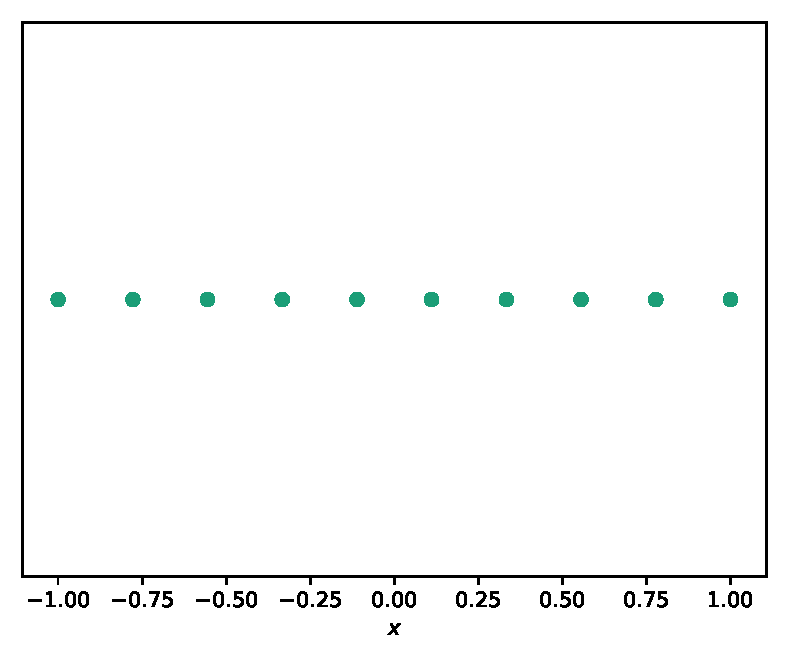
\includegraphics[width=0.47\textwidth]{figs/centers}
\par\end{centering}
}\hfill{}\subfloat[Standard RBFs]{\begin{centering}
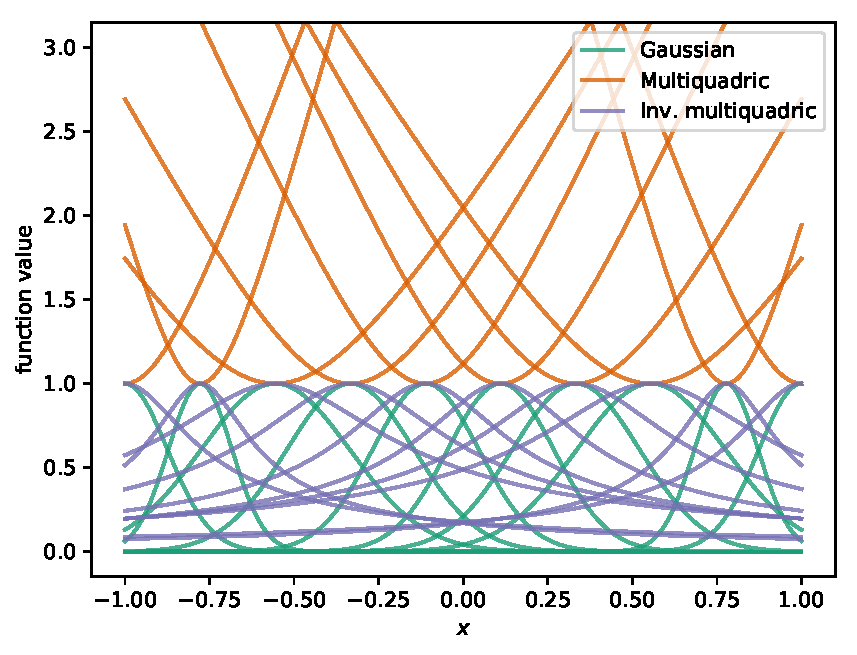
\includegraphics[width=0.47\textwidth]{figs/standard_functions}
\par\end{centering}
\label{fig:global-rbfs}}
\par\end{centering}
\begin{centering}
 \captionsetup{width=.4\linewidth}\subfloat[Wendland RBFs]{\begin{centering}
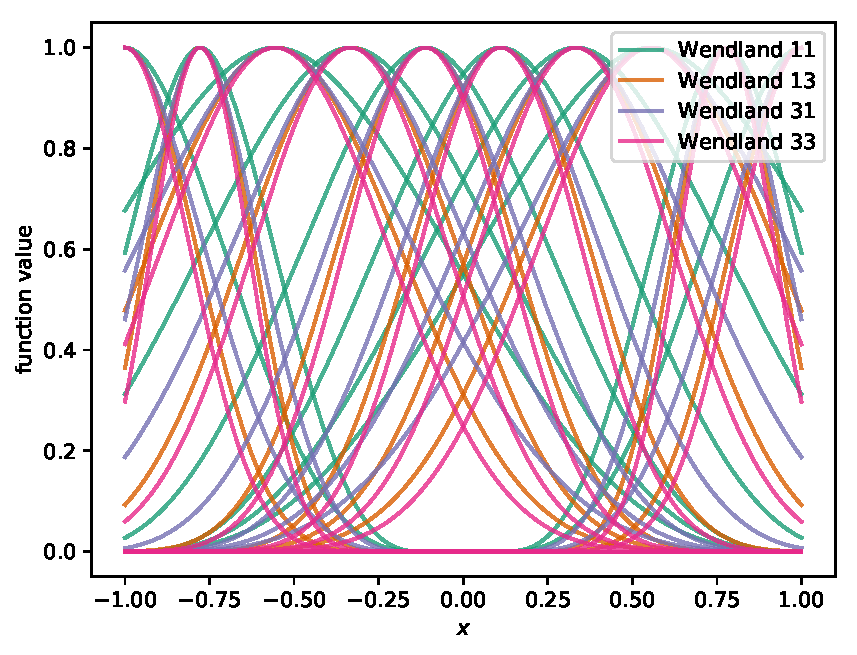
\includegraphics[width=0.47\textwidth]{figs/wendland_functions}
\par\end{centering}
\label{fig:wendland-1d}}\hfill{}\subfloat[Moving least squares functions with the original Wendland11 functions]{\begin{centering}
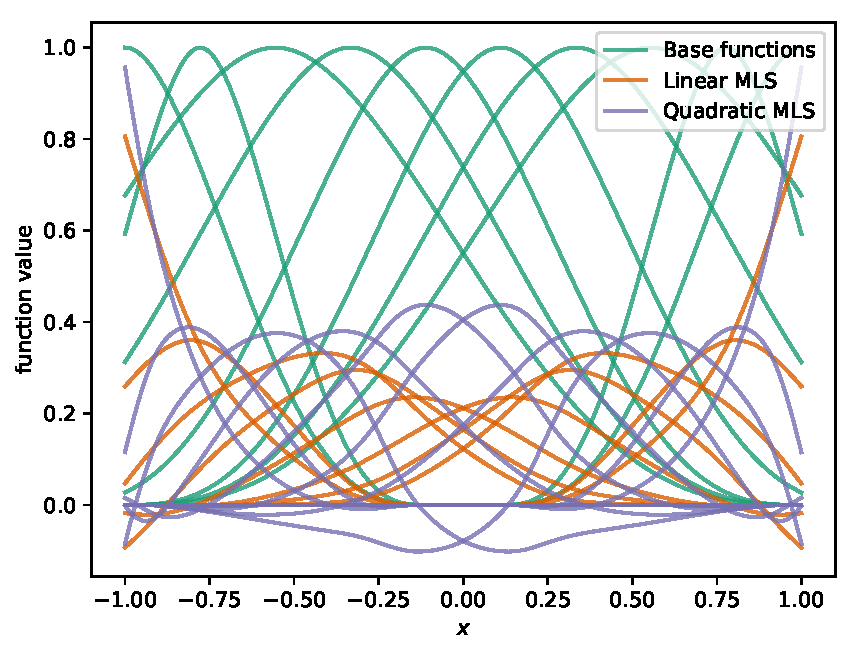
\includegraphics[width=0.47\textwidth]{figs/mls_functions}
\par\end{centering}
\label{fig:mls-1d}}
\par\end{centering}
\caption{Meshless functions in 1D for 10 equally-spaced center positions and
8 neighbors in radius calculation}
\label{fig:meshless-functions-1d}
\end{figure}

Figure \ref{fig:meshless-functions-1d} shows various meshless functions
for a simple set of equally-spaced centers in 1D. The standard \gls{rbf}
functions are global. The multiquadric functions in particular do
not converge to a finite limit as $r\to\infty$. Unlike the global
\gls{rbf}s, the Wendland \gls{rbf}s have a finite support radius.
Note, however, that like the standard \gls{rbf}s, the sum of these
functions is not equal to one at every point. This prevents proof
of neutron conservation (Sec. \ref{subsec:particle-balance}). Finally,
note the \gls{mls} functions in Fig. \ref{fig:mls-1d} that are created
using the initial basis of the Wendland 11 \gls{rbf}s in Fig. \ref{fig:wendland-1d}.
The sum of all the \gls{mls} functions at every point in the domain
is equal to one. The linear \gls{mls} functions are mostly positive
except near the boundaries, where they can go negative. The quadratic
\gls{mls} functions, on the other hand, have negative values for
much larger sections of the domain. Because of this, the results in
Chapters \ref{sec:method-of-manufactured}, \ref{sec:steady-results}
and \ref{sec:eigenvalue-results} use the linear \gls{mls} functions.
Empirical tests showed no improvement using the quadratic functions
instead of the linear functions in transport calculations. 

\cleardoublepage{}

\sectionspacing

\section{Implementation of meshless neutron transport\label{sec:methodology}}

The process of numerically solving the \gls{mlpg} form of the neutron
transport equations from Chapter \ref{sec:transport-discretization}
involves:
\begin{enumerate}
\item Creating the energy and angular discretizations (Sec. \ref{subsec:energy-angular-physical});
\item Creating the spatial discretization (Sec. \ref{subsec:spatial-discretization}),
including 
\begin{enumerate}
\item Defining the physical parameters of the system, such as the material
properties, boundary sources and problem dimensions;
\item Creating the weight functions; and
\item Performing integration of the basis and weight functions, the boundary
and internal sources and the cross sections (Chapter \ref{sec:integration-methods});
and
\end{enumerate}
\item Defining the operators representing the individual terms of the transport
equation and solving the resulting linear system of equations using
an appropriate solution technique (Sec. \ref{subsec:outer-iterations}). 
\end{enumerate}
This section discusses how these steps are optimized to keep the total
simulation cost reasonably low, including through parallelization
(Sec. \ref{subsec:parallelization}). Performance figures for the
\gls{mlpg} method are included in Sec. \ref{subsec:performance}. 

\subsection{Energy and angular discretization\label{subsec:energy-angular-physical}}

The independent variables for the energy discretization in the multigroup
equations include the number of energy groups and the upper and lower
energy bounds of each group. These parameters define which energies
each group represents in the integration of the the multigroup cross
sections, the source and the neutron flux (Sec. \ref{subsec:multigroup-transport-equation}).
If cross sections are generated through a Monte Carlo simulation,
these energies are used as the energy bounds for the energy tally.
For all of the problems in Chapters \ref{sec:method-of-manufactured},
\ref{sec:steady-results} and \ref{sec:eigenvalue-results}, the cross
sections are generated or chosen ahead of the meshless simulation
and the benchmark solutions (where applicable) are generated in multigroup
space. This is done to isolate the spatial discretization error, which
may be overshadowed by the error in converting the continuous-energy
cross sections to multigroup cross sections.

The independent variables for the angular discretization are the number
of scattering moments for the scattering cross section and the number
of directions for the discrete form of the solution. The number of
scattering moments defines the angular size of the scattering cross
section and the number of spherical harmonic moments. The directions
of flight $\bm{\Omega}_{n}$ are a set of integration ordinates on
the sphere. In one-dimensional Cartesian geometry, the angular dependence
is axially symmetric about the $x$ axis. Gauss-Legendre ordinates
and weights are used for the one-dimensional angular ordinates and
weights. In two-dimensional Cartesian geometry, the angular dependence
is symmetric about the $x-y$ plane. For the two- and three-dimensional
problems in this dissertation, the ordinates and weights for integration
over the unit sphere are from the \gls{ldfe} quadrature \cite{jarrell-discrete-2011}.
The discrete-ordinates assumption made for the angular discretization
in Sec. \ref{subsec:discrete-ordinates-transport} does not preclude
convergence to a continuous-in-angle solution. As the number of directions
increases, the error due to the angular discretization should decrease.

\subsection{Spatial discretization\label{subsec:spatial-discretization}}

In the discretized transport equations {[}Eq. (\ref{eq:full-transport}){]},
there are no constraints on the spatial dependence of the cross sections,
internal source and boundary sources. These values can be provided
directly as functions or, as in a Monte Carlo code, by a constructive
solid geometry (\gls{csg}). The \gls{csg} uses analytic surfaces
to define regions of (usually constant) material. For more information
the implementation of the \gls{csg}, see Appendix \ref{sec:constructive-solid-geometry}.
The manufactured solutions in Chapter \ref{sec:method-of-manufactured}
use functional forms for the cross sections, while the results for
more realistic problems in Chapters \ref{sec:steady-results} and
\ref{sec:eigenvalue-results} use a \gls{csg}. The full initialization
process for the spatial discretization is shown in Alg. \ref{alg:spatial-discretization}. 

\begin{algorithm}[!b]
\begin{algorithmic}[1] 
\State{\textbf{initialize} spatial discretization options}
\State{\textbf{read in} positions of the basis and weight function centers}
\State{\textbf{create} a k-d tree for distance calculations}
\State{\textbf{calculate} the radii of the meshless functions}
\State{\textbf{initialize} RBF functions}
\ForEach{basis or weight function $i$}
\State{\textbf{find} all other basis and weight functions that intersect with function $i$}
\State{\textbf{check} that no other centers are too close to the center of function $i$}
\EndFor
\State{\textbf{create} MLS functions using RBF functions}
\State{\textbf{create} the basis and weight functions using the MLS functions}
\State{\textbf{find} the basis and weight functions that intersect with the boundaries of the problem}
\State{\textbf{read in} cross sections and sources}
\State{\textbf{perform} basis and weight function integration}
\end{algorithmic}\caption{Initialization of the spatial discretization}
\label{alg:spatial-discretization}
\end{algorithm}


\subsubsection{Basis and weight functions\label{subsec:basis-and-weight}}

The centers of the basis and weight functions can be placed independently
of one another and of the problem geometry, with a few caveats. For
accurate representation of the solution, a higher concentration of
centers should be placed in areas where high gradients are expected.
If the weight function centers are placed too close together, the
equations are no longer be independent and the system is underdetermined,
while if the basis centers are placed too close together, the unknown
variables are no longer be independent and the system is overdetermined.
To prevent these issues, the code checks each basis and weight function
center for other centers that are too close. This is quantified for
each center by comparing the radius of the meshless function $r_{i}$
and the distance to the nearest other center $d_{i}^{\text{nearest}}$.
This is quantified in the code by a ratio of these two quantities,
which should be larger than a predefined tolerance $\epsilon$,
\[
\epsilon<\frac{d_{i}^{\text{nearest}}}{r_{i}},
\]
which for these calculations is defined to be $\epsilon=10^{-3}$.
For randomized points, this tolerance may need to be increased to
properly protect against an ill-conditioned set of points. 

The algorithm to calculate the radii of the basis and weight functions
is listed in Alg. \ref{alg:radius-calculation}. The purpose of the
algorithm is to ensure that at the center of each basis or weight
function, at least $N$ nearest points have a nonzero value. If the
point spacing is not too irregular (e.g. sets of isolated points that
don't ``see'' other any other sets), this also ensures basis and
weight function coverage throughout the problem domain. The connectivity
of the chosen points and radii is calculated using a k-d tree \cite{bentley-multidimensional-1975}
from nanoflann \cite{blanco-nanoflann:-2014}. To find which basis
functions overlap with each weight function, the weight function radius
is added to the maximum basis function radius in the problem and a
radius search is performed to find candidates for intersection, which
are then individually checked for actual intersection. 

\begin{algorithm}[!b]
\begin{algorithmic}[1] 
\State{\textbf{initialize} all radii to zero}
\ForEach{point $i$}
\State{\textbf{find} the nearest N neighboring points}
\ForEach{neighboring point $j$}
\State{\textbf{calculate} the distance from point $j$ to point $i$}
\If{current radius of point $j$ < distance to point $i$}
\State{\textbf{set} current radius of point $j$ = distance to point $i$}
\EndIf
\EndFor
\EndFor
\ForEach{point $i$}
\State{\textbf{multiply} the radius of point $i$ by a chosen scalar}
\EndFor
\end{algorithmic}\caption{Calculation of the support radii for the basis and weight functions}
\label{alg:radius-calculation}
\end{algorithm}

\begin{figure}[!tb]
\begin{centering}
 \captionsetup{width=.4\linewidth}\subfloat[Centers are placed at chosen locations in the domain and on its boundary.]{\begin{centering}
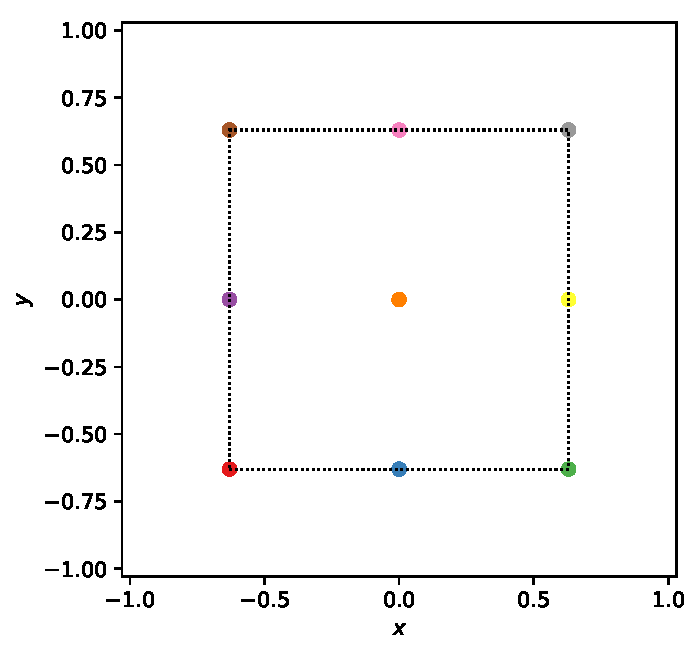
\includegraphics[width=0.47\textwidth]{figs/functions_square3_centers}
\par\end{centering}
}\hfill{}\subfloat[The radii are chosen such that a specified number of functions extend
to or past each point.]{\begin{centering}
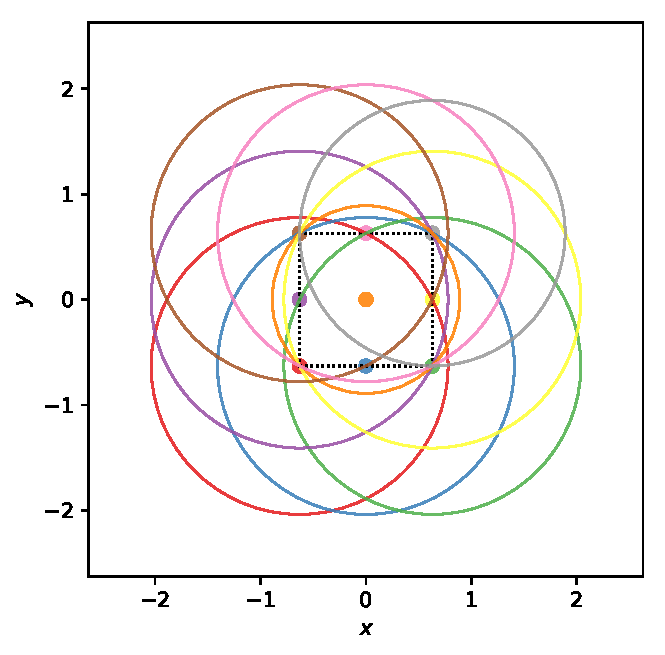
\includegraphics[width=0.47\textwidth]{figs/functions_square3_radii}
\par\end{centering}
\label{fig:meshless-function-radii}}
\par\end{centering}
\begin{centering}
 \captionsetup{width=.4\linewidth}\subfloat[A standard RBF basis using Wendland 11 functions is created using
the functions and radii. The functions are symmetric and do not sum
to a constant.]{\begin{centering}
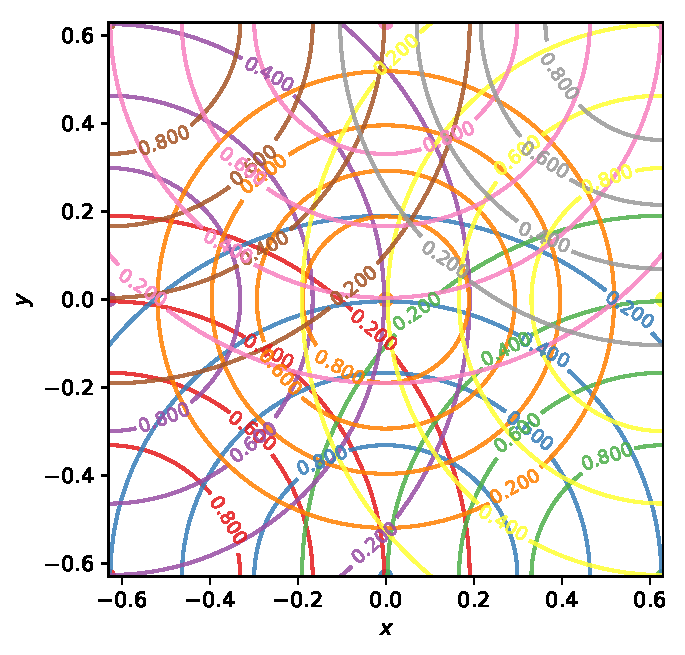
\includegraphics[width=0.47\textwidth]{figs/functions_square3_rbf}
\par\end{centering}
}\hfill{}\subfloat[Values of the linear MLS functions are calculated by normalizing the
RBF basis. The functions are asymmetric and sum to one at every point
in the domain. ]{\begin{centering}
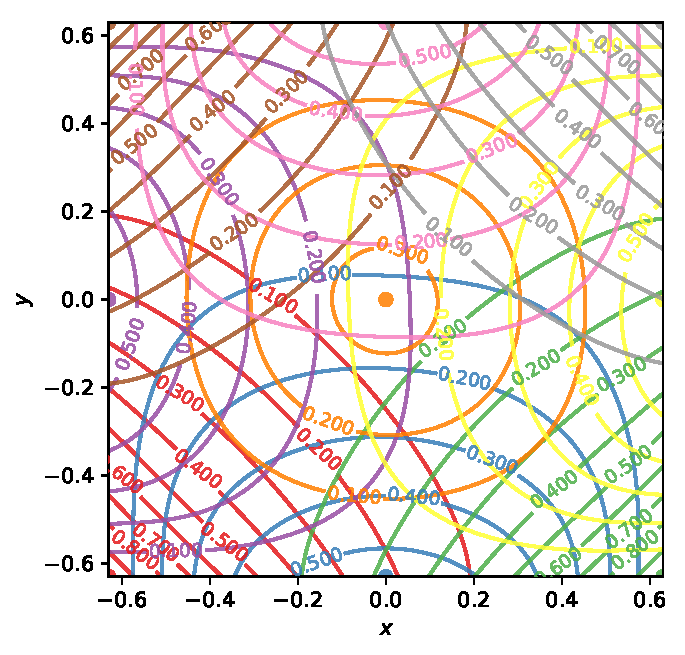
\includegraphics[width=0.47\textwidth]{figs/functions_square3_functions}
\par\end{centering}
\label{fig:mls-functions-2d}}
\par\end{centering}
\caption{Process of creating a set of MLS functions}
\label{fig:meshless-function-process}
\end{figure}

A one-dimensional plot of \gls{mls} functions with a Wendland function
basis in 1D is shown in Fig. \ref{fig:meshless-functions-1d}. The
process of creating a set of \gls{mls} functions is illustrated for
a 2D example in Fig. \ref{fig:meshless-function-process}. The centers
of the basis and weight functions are chosen to be a set of $3^{2}$
Cartesian points. The radii are calculated such that for each function,
eight total centers, including the center of the original function,
are included in or on the edge of the support radius. The standard
\gls{rbf} function basis is created with these support radii. As
in Fig. \ref{fig:wendland-1d}, these functions do not sum to one
at every point in the domain. Note that each \gls{rbf} function is
symmetric about its center. Using the original \gls{rbf} basis, the
values of the \gls{mls} functions can be calculated anywhere in the
domain. The values of these functions in Fig. \ref{fig:mls-functions-2d}
do sum to one at every point in the domain but are no longer symmetric
about the centers. 

Once a set of basis and weight functions is created, the integration
can be performed as described in Chapter \ref{sec:integration-methods}.
For the strong-form equations, the integration is only performed for
the basis function weighting {[}Eqs. (\ref{eq:strong-basis}){]},
as the point weighting uses cross sections evaluated at the collocation
points. The center points of the basis functions are also used as
the evaluation (or collocation) positions for the equations. Because
of this, a few additional constraints are placed on the placement
of the basis function centers for the strong form. First, there must
be points on the problem boundaries to satisfy the boundary conditions,
which unlike the weak form are not included in the transport equation.
Second, no boundary point should be on more than one boundary surface,
such as at a corner, as this would create a contradiction in the value
of the surface normal and definition of which points are upwind for
a chosen direction. The final constraint is the same as for the weak
form, namely that to avoid ill-conditioning, the basis function centers
should be placed as evenly as is practical for the problem geometry. 

\subsubsection{SUPG stabilization\label{subsec:supg-stabilization-implementation}}

The parameter that controls the addition of \gls{supg} stabilization
into the problem, $\tau$ from Eq. (\ref{eq:augmented-weight}), is
chosen to be weight-function dependent (i.e. $\tau\to\tau_{j}$) according
to the radius of the weight function $r_{j}$,
\begin{equation}
\tau_{j}=cr_{j},\label{eq:tau-radius}
\end{equation}
where $c$ is user-defined constant. With the shape parameter from
Eq. (\ref{eq:rbf-shape}), the \gls{rbf} value and derivative from
Eqs. (\ref{eq:rbf-basis}) and (\ref{eq:rbf-derivative}) and the
$\tau_{j}$ value from Eq. (\ref{eq:tau-radius}) with a dimensionless
support radius of $r_{sup}=1$, the \gls{supg}-augmented weight function
{[}Eq. (\ref{eq:augmented-weight}){]} becomes 
\begin{equation}
\tilde{w}_{j,n}=\Gamma\left(\epsilon_{j}d\left(\bm{x},\bm{x}_{i}\right)\right)+c\bm{\Omega}_{n}\cdot\left(\left[\bm{\nabla}d\left(\bm{x},\bm{x}_{i}\right)\right]\circ\left[\bm{\nabla}\Gamma\left(\epsilon_{j}d\left(\bm{x},\bm{x}_{i}\right)\right)\right]\right).\label{eq:explicit-supg-weight}
\end{equation}
Equation (\ref{eq:explicit-supg-weight}) shows that for the of $\tau_{j}$
in Eq. (\ref{eq:tau-radius}), the function-to-derivative ratio in
the stabilized weight function becomes independent of the weight function
radius $r_{j}$. A constant $\tau$ would add comparatively more numerical
diffusion for weight functions with smaller radii. This does mean
that the condition for conservation {[}Eq. (\ref{eq:augmented-weight-function-sum}){]}
is not preserved, as 
\begin{equation}
\sum_{j=1}^{J}\tau_{j}\bm{\Omega}_{n}\cdot\bm{\nabla}w_{j}\neq0
\end{equation}
in general, even where Eq. (\ref{eq:weight-function-sum}) holds.
However, in empirical tests, the weight function-dependent $\tau_{j}$
shows better performance and convergence for problems with varying
radii $r_{j}$ than a constant $\tau$. 

In both the full {[}Eqs. (\ref{eq:full-transport}){]} and basis {[}Eqs.
(\ref{eq:basis-transport}){]} fully-discretized equations, the moment-to-discrete
operator attached to the scattering, fission and implicitly the source
can be separated by separating the terms including $\tau$ from the
terms included in the transport equation without \gls{supg}. The
summation of the \gls{supg} terms is then performed using a modified
moment-to-discrete operator. This adds an additional index for the
gradient terms, which is $d$ in the following equations. For example,
for the ``full'' cross section equations, the scattering term becomes
\begin{equation}
\left(\mathcal{S}^{d}\beta\right)_{j,n,g,d}=\begin{cases}
\sum_{i=1}^{J}\sum_{g'=1}^{G}\overline{\Sigma}_{s;i,j,\ell,g'\to g}^{0}\beta_{i,\ell,g'}^{m}, & d=0,\\
\sum_{i=1}^{J}\sum_{g'=1}^{G}\left(\overline{\bm{\Sigma}}_{s;i,j,\ell,g'\to g}^{1}\right)_{d}\beta_{i,\ell,g'}^{m}, & d=1,2,3.
\end{cases}
\end{equation}
and the moment-to-discrete operator becomes 
\begin{equation}
\left(\mathcal{M}^{d}\beta\right)_{j,n,g}=\sum_{\ell=0}^{L}\frac{2\ell+1}{4\pi}\sum_{m=-\ell}^{\ell}Y_{\ell}^{m}\left(\bm{\Omega}_{n}\right)\sum_{d=0}^{3}f_{d}\tilde{\beta}_{j,\ell,g,d}^{m},
\end{equation}
where $\tilde{\beta}_{j,\ell,g,d}^{m}$ is the result of the $\mathcal{S}^{d}$
scattering operator and 
\begin{equation}
f_{d}=\begin{cases}
1, & d=0,\\
\tau\left(\bm{\Omega}_{n}\right)_{d}, & d=1,2,3.
\end{cases}
\end{equation}
With these definitions, $\mathcal{M}^{d}\mathcal{S}^{d}\beta=\left(\mathcal{M}\mathcal{S}^{p}\right)\beta$.
The results for the fission cross term directly follow. This same
method can be applied to the volume part of the source term,
\begin{equation}
\left(q_{V}^{d}\right)_{j,\ell,g,d}^{m}=\begin{cases}
\overline{Q}_{j,\ell,g}^{m,0}, & d=0,\\
\left(\overline{\bm{Q}}_{j,\ell,g}^{m,1}\right)_{d}, & d=1,2,3.
\end{cases}
\end{equation}
with the same moment-to-discrete operator. These optimizations cut
down on unnecessary computational cost in the scattering, fission
and internal source operators. 

\subsection{Streaming and collision operator\label{subsec:transport-sweep-operator}}

The $\mathcal{L}$ operator in both the weak and strong forms {[}Eqs.
(\ref{eq:streaming-petrov}) and (\ref{eq:strong-point-streaming}),
respectively{]} represents the application of a set of independent,
sparse matrices for each direction $n$ and energy group $g$, with
weighted equations corresponding to the rows. The number of nonzero
elements in each row $j$ is the number of basis functions that intersect
with the applicable weight function $w_{j}$. The $\mathcal{L}^{-1}$
operator, or the inverse of the $\mathcal{L}$ operator, is equivalent
to the solution of the system
\begin{equation}
\mathcal{L}\alpha=q\label{eq:linv-system}
\end{equation}
for the coefficients $\alpha$ given the vector $q$. The sparse $\mathcal{L}$
matrix reduces storage cost and permits the use of sparse linear algebra
packages to solve Eq. (\ref{eq:linv-system}). 

\subsubsection{Linear solver packages}

Several solvers from Trilinos \cite{heroux-overview-2005} are implemented
to solve the $\mathcal{L}^{-1}$ linear problem in Eq. (\ref{eq:linv-system}).
The KLU solver from Amesos uses the LU decomposition to directly solve
the $\mathcal{L}^{-1}$ problem. The direct solver is much more expensive
in memory and computational cost than iterative solvers and is not
generally needed for the weak-form equations with \gls{supg} stabilization.
The strong-form equations and the weak-form equations without \gls{supg}
stabilization have far worse conditioning without this diffusive stabilization
and generally do not work with iterative solvers. 

The Pseudo-Block generalized minimal residual (\gls{gmres}) solver
from the Belos package is used for iterative solution of the linear
problem. \gls{gmres} is a Krylov subspace method that relies on repeated
applications of the $\mathcal{L}$ operator {[}Eq. (\ref{eq:linv-system}){]}
to solve the linear problem. Because only the matrix and not its inverse
is used, the cost of the decomposition in a direct solve is allayed
and only the application of the $\mathcal{L}$ matrix is needed, not
the explicit matrix. This solver can be used without a preconditioner
for problems that are well-conditioned. For most problems, a preconditioner
improves the performance significantly. 

\subsubsection{Preconditioners\label{subsec:preconditioners}}

To improve the conditioning of the \gls{gmres} solution, a preconditioner
can be added to the problem. A preconditioner is an approximation
to the inverse of the original linear system, $\mathcal{L}^{-1}$.
Applying this preconditioner $\mathcal{P}^{-1}$ to both sides of
the original linear equation {[}Eq. (\ref{eq:linv-system}){]} results
in a left-preconditioned system,
\begin{equation}
\mathcal{P}^{-1}\mathcal{L}\alpha=\mathcal{P}^{-1}q.
\end{equation}
For a good choice of preconditioner, the combined matrix $\mathcal{P}^{-1}\mathcal{L}$
(which need not be explicitly formed) has a lower condition number
than the matrix $\mathcal{L}$. The simplest preconditioner is the
matrix $\mathcal{L}^{-1}$, which solves the system exactly in one
iteration but provides no speedup compared to using a direct solver.
A right-preconditioned system has a similar form,
\begin{equation}
\mathcal{L}\mathcal{P}^{-1}\mathcal{P}\alpha=q.
\end{equation}

These preconditioners are applied here using the ILUT (incomplete
LU decomposition with threshold) preconditioner from the Ifpack package
of Trilinos. Instead of storing the entire LU decomposition of the
preconditioner $\mathcal{P}$, which is much less sparse than the
original matrix, the ILUT decomposition instead stores an approximate
form of the LU decomposition. The ILUT preconditioner allows specification
of the level of fill and the drop tolerance of this approximate decomposition.
The level of fill controls to the number of elements kept in the decomposition
with respect to the original matrix. For a level of fill of 1.0, for
instance, the $\mathcal{P}^{-1}$ matrix has approximately the same
number of elements as the original $\mathcal{P}$ matrix. The dropping
technique of the ILUT preconditioner ensures that the remaining elements
of the approximate $\mathcal{P}^{-1}$ matrix are larger than the
drop tolerance. For most of the calculations in Chapters \ref{sec:method-of-manufactured},
\ref{sec:steady-results} and \ref{sec:eigenvalue-results}, the level
of fill is 1.0 and the drop tolerance is $10^{-12}$. 

To precondition the streaming operator, a suitable preconditioner
$\mathcal{P}$ must be defined. The most obvious option for a preconditioner
is to use the streaming operator matrix itself, $\mathcal{\mathcal{L=\mathcal{P}}}$,
and then let the ILUT preconditioner form an approximate inverse.
The $\mathcal{L}$ operation for the \gls{mlpg} transport equations
actually represents the application of linearly independent matrices
for each group and direction, which can be denoted as $\mathcal{L}_{n,g}$.
The ILUT preconditioner stores a separate ILUT approximation for these
preconditioners $\mathcal{P}_{n,g}^{-1}$ for each direction $n$
and group $g$. This is the preconditioner used for most of the results
in the following chapters, but this method does have major drawbacks
in memory cost. These preconditioners can be formed anew for each
$\mathcal{L}^{-1}$ application, but this requires an excessive amount
of computation that overshadows the benefits of the preconditioner. 

The second preconditioner implemented in the code relies on the assumption
that a solution for the angular flux values at the centers of the
weight functions, $\psi_{n,g}\left(\bm{x}_{j}\right)$, would be better-conditioned
than a solution for the coefficients of the basis function expansion
$\alpha_{i,n,g}$. The angular flux at the weight function centers
$\bm{x}_{j}$ is calculated from the basis function expansion as
\begin{equation}
\mathcal{B}\alpha=\psi,\label{eq:basis-preconditioner-values}
\end{equation}
where 
\begin{equation}
\mathcal{B}_{i,j,n,g}=b_{i}\left(\bm{x}_{j}\right).
\end{equation}
Solving Eq. (\ref{eq:basis-preconditioner-values}) for $\alpha$
and inserting this expansion into the $\mathcal{L}$ linear system
from Eq. (\ref{eq:linv-system}),
\begin{equation}
\mathcal{L}\mathcal{B}^{-1}\psi=q,
\end{equation}
results in an equation that solves for the angular flux at the weight
function centers. To convert back to a solution for the angular flux
expansion coefficients, the definition from Eq. (\ref{eq:basis-preconditioner-values})
is again applied to get
\begin{equation}
\mathcal{L}\mathcal{B}^{-1}\mathcal{B}\alpha=q,
\end{equation}
which is a right-preconditioned system for the $\mathcal{L}$ operator
with the preconditioner $\mathcal{B}$. Unlike the first preconditioner,
the matrix $\mathcal{B}$ is independent of both energy group and
direction. The storage cost is therefore negligible, which reduces
the memory requirements of solving the \gls{mlpg} transport equations
compared to the first preconditioner by one to two orders of magnitude.
However, because this preconditioner is not as good of an approximation
to the original $\mathcal{L}$ matrices, the number of \gls{gmres}
iterations required to converge the solution can increase significantly.
If the problem is solvable using \gls{gmres} without preconditioning,
this second preconditioner often takes as many iterations as the unpreconditioned
system, which indicates as expected that the preconditioner is not
a good approximation to the matrix. However, the preconditioner also
allows solution of problems that are too ill-conditioned for unpreconditioned
\gls{gmres}, which for these problems validates the assumption that
the solution for $\psi$ instead of $\alpha$ would improve the conditioning
of the solve.

\subsection{Iteration on the scattering and fission sources\label{subsec:outer-iterations}}

The streaming problem in Sec. \ref{subsec:transport-sweep-operator}
represents the solution for the angular flux for a given fixed neutron
source. To solve the full transport equation, an additional solution
step is required in iterating over the scattering and fission sources.
The steady-state and $k$-eigenvalue cases are considered separately.
For simplicity in notation, the Petrov-Galerkin superscripts from
Eqs. (\ref{eq:operator-petrov}) are dropped. 

\subsubsection{Steady-state outer iterations}

For a problem with no scattering or fission, the steady-state transport
equation {[}Eq. (\ref{eq:operator-steady-petrov}){]} becomes
\begin{equation}
\beta=\mathcal{D}\mathcal{L}^{-1}q\label{eq:purely-absorbing-operator}
\end{equation}
and a single application of the $\mathcal{L}^{-1}$ operator produces
the solution. Equation (\ref{eq:purely-absorbing-operator}) represents
the first-flight source, or the source neutrons that have not interacted
with the material. If there are reflective boundaries in the problem,
a simple source iteration scheme is used to converge on the first-flight
source, which includes neutrons that have been reflected but have
not interacted with the material. After the neutrons have interacted
with the material, they may scatter or produce fission neutrons. The
neutrons from these subsequent generations are added to the first-flight
source to calculate the full solution to the neutron transport equation.
The iterations over the scattering and fission sources, referred to
as the outer iterations, can be done directly through source (or Richardson)
iteration,
\begin{equation}
\beta^{\ell+1}=\mathcal{D}\mathcal{L}^{-1}\mathcal{M}\left(\mathcal{S}+\mathcal{F}\right)\beta^{\ell}+\mathcal{D}\mathcal{L}^{-1}q,\label{eq:source-iteration}
\end{equation}
where the index $\ell$ refers to the iteration. This iteration process
is continued until the solution $\beta$ converges to a chosen tolerance.
The source iteration equation updates the scattering and fission sources
for each subsequent generation of neutrons. If the initial guess for
the solution is $\beta^{1}=\mathcal{D}\mathcal{L}^{-1}q$, then $\beta^{\ell}$
represents the $\ell^{th}$ flight neutrons. For problems with high
scattering ratios where the neutrons may scatter hundreds of times
before leaving the problem through absorption or leakage, source iteration
is not ideal as it requires an iteration to simulate each generation
of neutrons. 

The Krylov solvers discussed in Sec. \ref{subsec:transport-sweep-operator}
provide a simple way to speed up the calculations. Eq. (\ref{eq:source-iteration})
can be rewritten into the form used throughout Chapter \ref{sec:transport-discretization},

\begin{equation}
\left[\mathcal{I}-\mathcal{D}\mathcal{L}^{-1}\mathcal{M}\left(\mathcal{S}+\mathcal{F}\right)\right]\beta=\mathcal{D}\mathcal{L}^{-1}q,
\end{equation}
and solved by applying a \gls{gmres} solver to invert the combined
operator on the lefthand side of the equation. The combined operator
does not need to be formed explicitly, as \gls{gmres} only requires
the action of the operator. For the solution of this system, the code
uses AztecOO, which is another Trilinos package, without preconditioning.
Preconditioners such as diffusion synthetic acceleration \cite{alcouffe-diffusion-1977}
have been successfully applied to speed up convergence of the scattering
and fission sources for various other transport discretizations, but
are not investigated here for the \gls{mlpg} equations. 

\subsubsection{Eigenvalue outer iterations}

The standard operator form of the $k$-eigenvalue equation {[}Eq.
(\ref{eq:k-eigenvalue}){]} for the coefficients $\beta$ is written
\begin{equation}
\mathcal{L}\beta=\mathcal{M}\left(\mathcal{S}+\frac{1}{k}\mathcal{F}\right)\mathcal{D}\beta,
\end{equation}
where again the operators convert from the coefficients to the physical
neutron flux where appropriate. One method of solving this equation
is fixed point iteration, which updates the coefficients using a similar
process to source iteration,\begin{subequations}
\begin{equation}
\beta^{\ell+1}=\mathcal{D}\mathcal{L}^{-1}\mathcal{M}\left(\mathcal{S}+\frac{1}{k^{\ell}}\mathcal{F}\right)\beta^{\ell}.
\end{equation}
After each iteration, the eigenvalue is updated as
\begin{equation}
k^{\ell+1}=\frac{\left\Vert \mathcal{F}\beta^{\ell+1}\right\Vert }{\left\Vert \frac{1}{k}\mathcal{F}\phi^{\ell}-\mathcal{S}\left(\beta^{\ell+1}-\beta^{\ell}\right)\right\Vert },
\end{equation}
\end{subequations}where the norm $\left\Vert \left(\cdot\right)\right\Vert $
represents a volume summation or integral \cite{calef-nonlinear-2013}.
Power iteration, which is more costly per iteration than fixed point
iteration but also more stable, is written as\begin{subequations}
\begin{equation}
\beta^{\ell+1}=\left(\mathcal{I}-\mathcal{D}\mathcal{L}^{-1}\mathcal{M}\mathcal{S}\right)^{-1}\mathcal{D}\mathcal{L}^{-1}\mathcal{M}\frac{1}{k}\mathcal{F}\beta^{\ell},
\end{equation}
while the update of the eigenvalue takes the form
\begin{equation}
k^{\ell+1}=\frac{\left\Vert \mathcal{F}\beta^{\ell+1}\right\Vert }{\left\Vert \frac{1}{k^{\ell}}\mathcal{F}\beta^{\ell}\right\Vert }.
\end{equation}
\end{subequations}The $\left(\mathcal{I}-\mathcal{D}\mathcal{L}^{-1}\mathcal{M}\mathcal{S}\right)^{-1}$
term in the power iteration represents the solution of a steady-state
transport problem 
\begin{equation}
\left(\mathcal{I}-\mathcal{D}\mathcal{L}^{-1}\mathcal{M}\mathcal{S}\right)\beta=s,
\end{equation}
where $s$ is the given source. Thus, each power iteration requires
a full steady-state solution when using power iteration.

Similar to the steady-state equation, the $k$-eigenvalue problem
can be solved more efficiently by using Krylov iterative methods.
For a Krylov solver that requires isolation of the eigenvalue (such
as Block Krylov-Schur), the Krylov iteration can be written as 
\begin{equation}
\left(\mathcal{I}-\mathcal{D}\mathcal{L}^{-1}\mathcal{M}\mathcal{S}\right)^{-1}\mathcal{D}\mathcal{L}^{-1}\mathcal{M}\mathcal{F}\beta=k\beta,
\end{equation}
where again a full steady-state problem must be solved for each eigenvalue
iteration. Generalized eigensolvers reduce the cost further by supporting
an operator on the eigenvalue side of the equation,
\begin{equation}
\mathcal{D}\mathcal{L}^{-1}\mathcal{M}\mathcal{F}\beta=k\left(\mathcal{I}-\mathcal{D}\mathcal{L}^{-1}\mathcal{M}\mathcal{S}\right)\beta.
\end{equation}
This form of the eigenvalue equation is solved here with unpreconditioned
Generalized Davidson using Anasazi, another Trilinos package. This
significantly reduces computational cost compared to the other eigensolvers
\cite{hamilton-numerical-2011}. 

\subsection{Parallelization\label{subsec:parallelization}}

The code for the \gls{mlpg} equations uses OpenMP \cite{dagum-openmp-1998}
to implement thread-level parallelization. For the meshless integration
technique (Sec. \ref{subsec:meshless-integration}) the independence
of the integrals for each weight function allows for parallel integration.
For the background integration technique (Sec. \ref{subsec:background-mesh-integration}),
the integration is parallelized for the background cells and surfaces.
As the basis and weight functions are not exclusive to a single background
cell, each thread receives its own copy of the integrals. After the
integration is complete for all threads, these integrals are summed
together, which produces the full integral of each basis and weight
function over the entire problem domain. Due to the adaptive integration
technique introduced in Sec. \ref{subsec:background-mesh-integration},
the time required to integrate the basis and weight functions over
each cell is not constant. As such, the scheduling of the parallel
integration is dynamic. 

The operators such as $\mathcal{D}$, $\mathcal{M}$, $\mathcal{S}$
and $\mathcal{F}$ are parallelized for the spatial index. For instance,
the weighted fission sources for the weight functions $w_{j}$ are
calculated in parallel. Because of the shared-memory model, the overlap
of the basis function coefficients between the various weighted fission
sources is not an issue. 

If directionally-dependent preconditioners (Sec. \ref{subsec:preconditioners})
are used, their \gls{ilut} decomposition is computed in parallel.
If the preconditioners are independent of direction, each thread computes
and uses a separate copy of the preconditioner. The streaming and
collision operator is independent for each group and direction and
is parallelized in direction. The \gls{gmres} operator that performs
the outer iterations does not occupy a large percentage of the computational
time and is not parallelized. 

For extension to a higher number of processors than one node, the
Trilinos linear algebra packages used for the outer and inner transport
iterations support fully parallel computations using MPI. The weighting
of the solution coefficients to calculate the scattering and fission
sources and the $\mathcal{L}^{-1}$ operator are the two places where
the code requires communication between different spatial points,
and these could be parallelized using MPI for the communication and
Trilinos for the parallel linear solution of the equations. 

\subsection{Performance figures from results\label{subsec:performance}}

The meshless method trades flexibility in geometric specification
for computational cost. The main contributors to higher computational
cost are the integration step and the initialization and application
of the matrices representing the $\mathcal{L}^{-1}$ operation for
each direction and energy group. Unlike mesh-based methods, which
usually have constant material parameters in each cell and use simple
polynomial basis functions, the presented method must query the \gls{csg}
for material properties and uses functions that require many quadrature
points to integrate accurately. The number of basis functions at each
integration point ranges from 10\textendash 30 in 2D to 20\textendash 90
in 3D. Each of these basis functions is expensive to calculate in
comparison to a polynomial, particularly when using an \gls{mls}
basis {[}see Eqs. (\ref{eq:mls-value}) and (\ref{eq:mls-derivative}){]}.
The integrals must simultaneously converge over the cross sections
and the basis and weight functions, making problems such as the \gls{ifba}
pincell problem (Sec. \ref{subsec:vera}) with discontinuous cross
sections and radii that vary over more than an order of magnitude
difficult to integrate accurately (Sec. \ref{subsec:vera-pincell-integration}). 

The performance of the code is measured for several of the problems
as specified in Chapters \ref{sec:steady-results} and \ref{sec:eigenvalue-results}.
While the base cost of the \gls{mlpg} method is high, the time and
memory required scales approximately linearly with the number of points
for any given problem. Table \ref{tab:scaling} shows the results
of an empirical fit of the timing and memory data to the number of
points. The solve scales near-linearly for the problems considered.
The exception to the linear scaling is the initialization time of
the native \gls{ilut} preconditioners for the $\mathcal{L}^{-1}$
matrices in three dimensions, which scales approximately as $N^{1.5}$
for the number of points $N$. 

\begin{table}[!b]
\caption{Empirical scaling of memory and timing with number of points $N$
with native \gls{ilut} preconditioner}

\centering{}%
\begin{tabular}{|c|c|cc|c|}
\hline 
\multicolumn{2}{|c|}{Scaling parameter} & \multicolumn{1}{c|}{1D} & 2D & 3D\tabularnewline
\hline 
\hline 
\multicolumn{2}{|c|}{Memory} &  & \multicolumn{1}{c}{} & \tabularnewline
\cline{1-2} 
\multirow{3}{*}{Timing} & Integration &  & \multicolumn{1}{c}{$\sim N$} & \tabularnewline
\cline{2-2} \cline{5-5} 
 & $\mathcal{L}^{-1}$ initialization &  &  & $\sim N^{1.5}$\tabularnewline
\cline{2-2} \cline{4-5} 
 & Solve & \multicolumn{1}{c|}{} & $\sim N^{1.15}$ & $\sim N^{1.2}$\tabularnewline
\hline 
\end{tabular}\label{tab:scaling}
\end{table}

Values for the timing and memory requirements for sample problems
that have around 5000 points are shown in Table \ref{tab:performance-figures}.
Most of the timing values are highly problem-dependent. The \gls{vera}
pincell cases have similar integration times to the 3D problems due
to the geometric complexity and small basis and weight function radii
near the fuel boundary. The pincell problems have no leakage and low
absorption outside of the \gls{ifba} region in the thermal group,
which means the boundary source takes many iterations to converge.
Adjusting for the number of points, each iteration for the \gls{vera}
and \gls{icsbep} problems takes approximately the same time. 

\begin{table}[!tb]
\caption{Example performance figures using four processors with standard ILUT
preconditioner}

\centering{}%
\begin{tabular}{|c|c|c|c|c|c|c|}
\hline 
\multicolumn{2}{|c|}{Parameter} & Slab 1D & \gls{vera} 1B & \gls{vera} 1E & Kobayashi & \gls{icsbep}\tabularnewline
\hline 
\hline 
\multicolumn{2}{|c|}{Problem type} & Fixed & Eigenvalue & Eigenvalue & Fixed & Eigenvalue\tabularnewline
\hline 
\multicolumn{2}{|c|}{Spatial dimensions} & 1 & 2 & 2 & 3 & 3\tabularnewline
\hline 
\multicolumn{2}{|c|}{Num. points} & 5120 & 5556 & 5439 & 4913 & 4998\tabularnewline
\hline 
\multicolumn{2}{|c|}{Num. directions} & 256 & 256 & 256 & 512 & 512\tabularnewline
\hline 
\multicolumn{2}{|c|}{Num. groups} & 2 & 2 & 2 & 1 & 1\tabularnewline
\hline 
\multicolumn{2}{|c|}{Num. integration cells} & 5000 & 16384 & 16384 & 8000 & 4160\tabularnewline
\hline 
\multicolumn{2}{|c|}{Num. quadrature points per cell} & 16 & 256\textendash 1024 & 256\textendash 12544 & 512 & 1728\tabularnewline
\hline 
\multicolumn{2}{|c|}{Memory (GB)} & 1.48 & 2.79 & 3.24 & 4.99 & 5.01\tabularnewline
\hline 
\multicolumn{2}{|c|}{Number of iterations} & 16 & 52 & 46 & 19 & 20\tabularnewline
\hline 
\multirow{4}{*}{Timing (sec)} & Total & 37 & 330 & 751 & 427 & 767\tabularnewline
\cline{2-7} 
 & Integration & 1 & 59 & 480 & 232 & 568\tabularnewline
\cline{2-7} 
 & $\mathcal{L}^{-1}$ initialization & 11 & 29 & 59 & 123 & 116\tabularnewline
\cline{2-7} 
 & Solve & 24 & 241 & 211 & 71 & 83\tabularnewline
\hline 
\end{tabular}\label{tab:performance-figures}
\end{table}

Storage of the native \gls{ilut} preconditioners for each direction
and group represents most of the high memory cost. The computational
cost of initializing the \gls{ilut} preconditioners makes recomputation
at each application of the $\mathcal{L}^{-1}$ operator impractical.
For details on the memory usage and computational cost of the two
preconditioners, see Sec. \ref{subsec:preconditioner-performance}.

\subsubsection{Parallel performance}

Due to the shared-memory model of the \gls{mlpg} code, the number
of processors for which the code can be tested is limited. The parallelism
does not involve heavy communication between processes for the parallel
portions of the code, so good efficiency is expected for these portions
of the code. However, there are some sections of the code, including
the initialization of the spatial geometry and the outer \gls{gmres}
solver, are run in serial and could have an impact on parallel performance.
The code is not heavily optimized for parallel performance, and so
while these results do show good speedup for some cases, near-optimal
speedup is not expected. 

To test the parallel performance, the Kobayashi problem from Sec.
\ref{subsec:kobayashi} with scattering is run in parallel for 1,
2, 4 and 8 processors for between 1000 and 64000 points with the same
problem parameters as in Table \ref{tab:general-parameters-steady},
except with 128 directions to decrease the total runtime of the parallel
tests. The efficiency of the parallelism is calculated as
\begin{equation}
E_{p}=\frac{T_{1}}{pT_{p}},
\end{equation}
where $T_{p}$ is the execution time of the problem on $p$ processors.
The efficiency is calculated for each of the spatial initialization
step (which is dominated by the integration of the basis and weight
functions), the initialization of the preconditioners and solution
of the operator equations, and the total time. 

Figure \ref{fig:parallel-efficiency-kobayashi-mls} shows the parallel
efficiency for the simulation using linear \gls{mls} functions created
from a Wendland 11 basis. The preconditioner initialization has near-optimal
efficiency as no communication between the processes is needed. The
solution of the problem falls off in efficiency as the number of processors
increases, from around 80 percent for 4 processors to 50 percent for
8 processors. This is possibly due to the serial sections of code
in the solution step. The integration step of the spatial initialization
does not involve heavy communication between processors or long serial
sections, so the drop in efficiency signals that the integration step
is likely slowed by either shared data access between processors due
to the interdependent \gls{mls} functions or by the disparity in
calculation times for \gls{mls} functions with few or many Wendland
basis functions. 

\begin{figure}[!tb]
\begin{centering}
\subfloat[Spatial initialization]{\begin{centering}
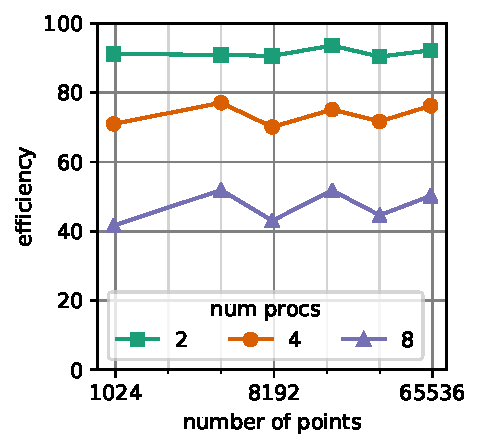
\includegraphics[width=0.23\textwidth]{figs/kobayashi_efficiency_mls_weak_init}
\par\end{centering}
}\subfloat[Preconditioner initialization]{\begin{centering}
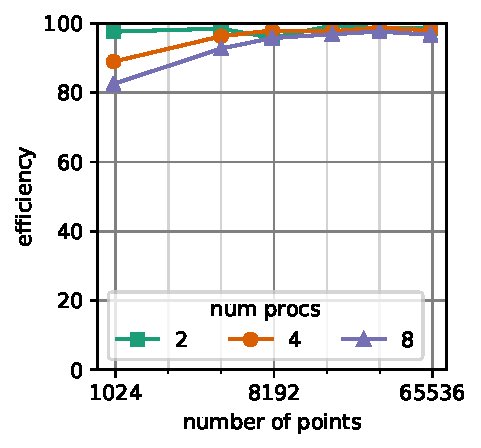
\includegraphics[width=0.23\textwidth]{figs/kobayashi_efficiency_mls_solve_init}
\par\end{centering}
}\subfloat[Solution]{\begin{centering}
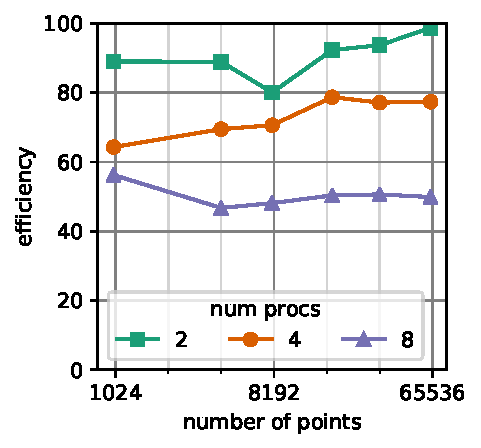
\includegraphics[width=0.23\textwidth]{figs/kobayashi_efficiency_mls_solve}
\par\end{centering}
}\subfloat[Total]{\begin{centering}
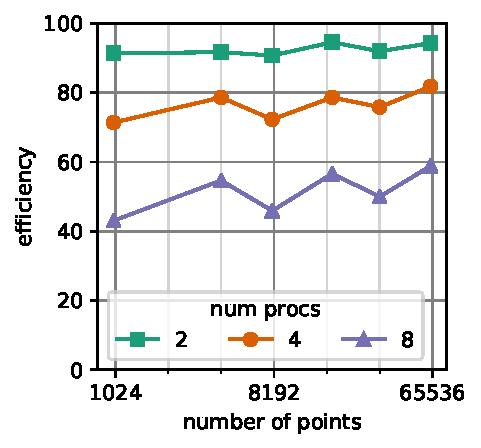
\includegraphics[width=0.23\textwidth]{figs/kobayashi_efficiency_mls_total}
\par\end{centering}
}
\par\end{centering}
\caption{Parallel efficiency for the Kobayashi problem with scattering, linear
MLS functions}

\label{fig:parallel-efficiency-kobayashi-mls}
\end{figure}

\begin{figure}[!tb]
\begin{centering}
\subfloat[Spatial initialization]{\begin{centering}
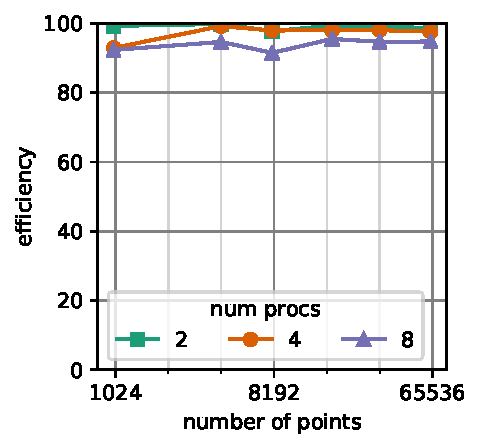
\includegraphics[width=0.23\textwidth]{figs/kobayashi_efficiency_rbf_weak_init}
\par\end{centering}
}\subfloat[Preconditioner initialization]{\begin{centering}
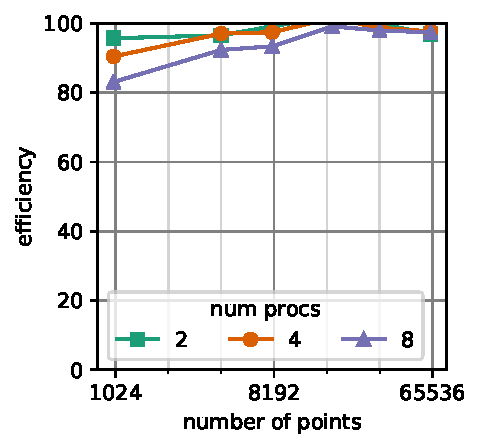
\includegraphics[width=0.23\textwidth]{figs/kobayashi_efficiency_rbf_solve_init}
\par\end{centering}
}\subfloat[Solution]{\begin{centering}
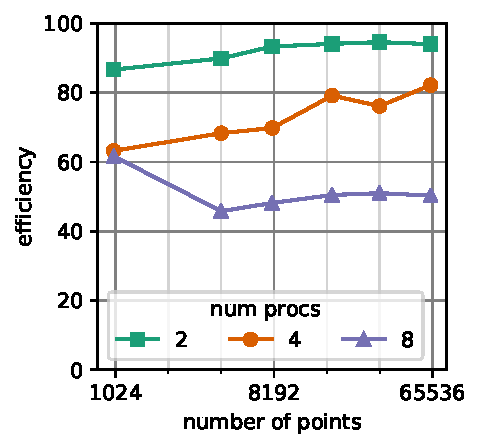
\includegraphics[width=0.23\textwidth]{figs/kobayashi_efficiency_rbf_solve}
\par\end{centering}
}\subfloat[Total]{\begin{centering}
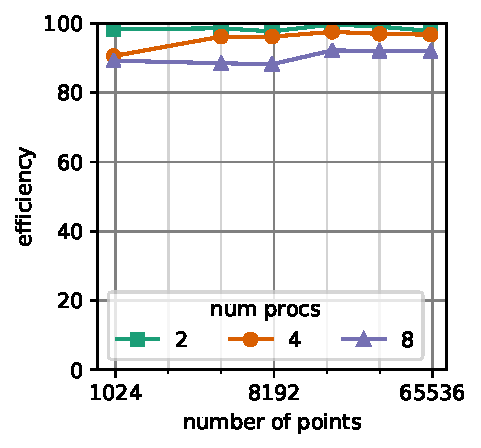
\includegraphics[width=0.23\textwidth]{figs/kobayashi_efficiency_rbf_total}
\par\end{centering}
}
\par\end{centering}
\caption{Parallel efficiency for the Kobayashi problem with scattering, RBF
functions}

\label{fig:parallel-efficiency-kobayashi-rbf}
\end{figure}

The same study with the same problem and parameters is done for the
Wendland 11 functions without linear \gls{mls} normalization. In
Fig. \ref{fig:parallel-efficiency-kobayashi-rbf}, the preconditioner
initialization and solution show similar results, but the spatial
initialization efficiency becomes near-optimal, at over 90 percent
efficiency for all choices of number of processors and points. The
only difference between these two studies is the normalization of
the linear \gls{mls} functions, which significantly slows parallel
performance. It is likely that with optimization the linear \gls{mls}
functions could be calculated in parallel with similar efficiency.
Because the integration step is more efficient, the total parallel
efficiency is near-optimal for this problem. For a problem with a
scattering source that is more difficult to converge, the suboptimal
solution efficiency would reduce the total efficiency. 

\subsubsection{Preconditioner performance\label{subsec:preconditioner-performance}}

The native \gls{ilut} preconditioner works well for most problems
as long as the radii of the basis and weight functions are not too
large. The fill level of the $\mathcal{L}^{-1}$ matrices can be increased
to compensate for larger radii, but at the cost of computational performance.
From empirical tests, if the problem does not converge for a fill
level of 1.0, then it is likely that the point setup itself is too
irregular (see Sec. \ref{subsec:basis-and-weight}), the \gls{supg}
parameter for numerical diffusion is too low (Sec. \ref{subsec:supg-stabilization-implementation})
or the chosen radii of the basis and weight functions is too large.
Generally, the native preconditioner reduces the required number of
inner iterations from several hundred to around 4 to 10. 

\begin{table}[!b]
\caption{Preconditioner performance for VERA 1E problem with 4 processors,
3522 points and 256 directions}
\label{tab:vera-preconditioner}
\centering{}%
\begin{tabular}{|c|c|c|c|c|c|c|}
\hline 
Preconditioner & Num. precs. & Memory & Prec. init. & Solve & Outer & Inner\tabularnewline
\hline 
\hline 
Basis function & 1 & 0.549 GB & 6.6 sec & 3164.3 sec & 45 & 475\textendash 668\tabularnewline
\hline 
Native & 512 & 3.017 GB & 56.7 sec & 348.9 sec & 45 & 7\textendash 8\tabularnewline
\hline 
None & 0 & \multicolumn{5}{c|}{does not converge}\tabularnewline
\hline 
\end{tabular}
\end{table}

The basis function value preconditioner does not work as reliably
well as the native preconditioner and requires many more iterations
to converge as it is not a good approximation to the original $\mathcal{L}$
matrix, as discussed in Sec. \ref{subsec:preconditioners}. For instance,
for an \gls{ifba} pincell (Sec. \ref{subsec:vera}) with 3522 points
and 256 directions on 4 processors, the native preconditioner requires
57 seconds to initialize the preconditioner matrices and 349 seconds
to solve the full operator equations, while the basis function preconditioner
requires 7 seconds to initialize the preconditioner matrices and 3164
seconds to solve the equations (Table \ref{tab:vera-preconditioner}).
This appears to be almost entirely due to a larger number of \gls{gmres}
iterations to solve the $\mathcal{L}^{-1}$ system. However, the basis
function preconditioner requires much less memory, at 0.55 GB instead
of 3.02 GB. For problems with more directions and energy groups, the
difference in memory usage is correspondingly larger, as the basis
function preconditioner scales only with the number of points, whereas
the native preconditioner scales linearly with the product of the
number of points, directions and groups. For this problem, the \gls{gmres}
solver without a preconditioner does not converge. 

\begin{table}[t]
\caption{Preconditioner performance for Kobayashi problem with 8 processors,
64000 points and 512 directions}
\label{tab:kobayashi-preconditioner}
\centering{}%
\begin{tabular}{|c|c|c|c|c|c|c|}
\hline 
Preconditioner & Num. precs. & Memory, (basis / full) & Prec. init. & Solve & Outer & Inner\tabularnewline
\hline 
\hline 
Basis function & 1 & \multicolumn{5}{c|}{does not converge}\tabularnewline
\hline 
Native & 512 & 72 / 75 GB & 1037.3 sec & 251.9 sec & 20 & 6\textendash 10\tabularnewline
\hline 
None & 0 & 4 / 7 GB & 0.0 sec & 2826.7 sec & 20 & 93\textendash 154\tabularnewline
\hline 
\end{tabular}
\end{table}

There also exist problems for which the basis function preconditioner
does not work well. For instance, for the partially-scattering Kobayashi
problem (Sec. \ref{subsec:kobayashi}) with 64000 points and 512 directions,
the $\mathcal{L}^{-1}$ operation with the basis function preconditioner
does not converge within 8000 \gls{gmres} iterations for some directions.
However, for this problem the \gls{gmres} method without preconditioning
does converge (see Table \ref{tab:kobayashi-preconditioner}). On
8 processors, the \gls{ilut} method requires 1037 seconds to initialize
the preconditioner matrices and 251 seconds to solve the problem.
The \gls{gmres} method without a preconditioner requires no time
to initialize the preconditioner matrices and 2826 seconds to solve
the problem. For this problem, then, the total cost of the initialization
and solution steps is around twice as high for the solver without
preconditioning. This problem requires around 20 applications of the
$\mathcal{L}^{-1}$ operator. For a problem that requires many more
applications of this operator, such as a problem with high scattering
ratios, the fixed cost of initialization of the \gls{ilut} matrices
and low cost of the solution step for the preconditioned system would
be much more efficient. 

For the Kobayashi problem, the memory required to perform the simulation
with preconditioning is around 75 GB, most of which is the storage
of the \gls{ilut} preconditioners. This memory cost scales approximately
linearly with the product of the number of angles, groups and points.
The memory cost of the simulation without preconditioning is around
7 GB, much of which is the storage of the integrated cross sections.
For the basis function cross section weighting, the memory usage decreases
to around 4 GB. The memory cost scales linearly with the product of
the number of groups and points. An empirical equation for the memory
in GB for the two solution techniques applied to the Kobayashi problem
is
\begin{align}
M_{\text{no prec}} & \approx\begin{cases}
6.3\times10^{-5}J, & \text{basis weighting},\\
1.1\times10^{-4}J, & \text{full weighting},
\end{cases}\\
M_{\text{prec}} & \approx M_{\text{no prec}}+2.1\times10^{-6}JN,
\end{align}
where $J$ is the number of spatial points and $N$ is the number
of directions. The scaling of the preconditioned method with the number
of directions makes simultaneous angular and spatial convergence difficult
to achieve, but the solution without preconditioning does not converge
for many problems, including the \gls{vera} problem mentioned earlier
in this section. 

Section \ref{subsec:future-work} discusses the need for more efficient
solution methods for the $\mathcal{L}^{-1}$ operation. Better preconditioners
would significantly reduce the computational cost and memory requirements
for the \gls{mlpg} method as presented here. 

\cleardoublepage{}

\sectionspacing

\section{Integration methods for meshless transport\label{sec:integration-methods}}

Once the connectivity of the basis and weight functions is determined
as described in Sec. \ref{subsec:spatial-discretization}, the integration
{[}e.g. in Eqs. (\ref{eq:supg-petrov-galerkin}), (\ref{eq:sigma_t-full}),
(\ref{eq:sigma_f-full}) and (\ref{eq:sigma_t-basis}){]} is performed
using one of two methods, a meshless integration technique (Sec. \ref{subsec:meshless-integration})
or a background mesh (Sec. \ref{subsec:background-mesh-integration}).
The domain of integration for the \gls{mlpg} discretization is defined
by the region of support of the basis and weight functions. For the
functions described in Sec. \ref{subsec:meshless-functions}, the
support region of each basis or weight function is a circle in 2D
or a sphere in 3D. The region of support for the intersection of a
basis and weight function is often a 2D or 3D lens. These geometries
are complicated somewhat by the addition of boundaries, which limit
the region of support to the physical problem domain. 

An integral over the region $R$ can be performed numerically as
\begin{equation}
\int_{R}f\left(\bm{x}\right)dV=\sum_{i}c_{i}f\left(\bm{x}_{i}\right),
\end{equation}
where $c_{i}$ are the integration weights and $\bm{x}_{i}$ are the
integration ordinates. One method of calculating the integration ordinates
and weights is by using a tensor product quadrature. Starting with
two integration quadratures for the integrals over $x$ and $y$ (with
the ordinates and weights $x_{i}$, $y_{j}$, $c_{i}^{x}$, $c_{j}^{y}$),
the tensor-product quadrature over a 2D Cartesian region with the
limits $x\in R_{x}$ and $y\in R_{y}$ can be written as\begin{subequations}
\begin{equation}
\int_{R_{y}}\int_{R_{x}}f\left(\bm{x}\right)dxdy=\sum_{i,j}c_{i,j}f\left(\bm{x}_{i,j}\right),
\end{equation}
where
\begin{gather}
\bm{x}_{i,j}=\left(x_{i},y_{j}\right),\\
c_{i,j}=c_{i}^{x}c_{j}^{y}.
\end{gather}
\end{subequations}Integrals for the geometries described in Secs.
\ref{subsec:meshless-integration} and \ref{subsec:background-mesh-integration}
can be done in the same way. 

\subsection{Meshless integration\label{subsec:meshless-integration}}

The first integration method performs the integrals numerically over
the region of support of the basis and weight functions. Similar methods
are used in Refs. \cite{de-method-2001,madhavan-numerical-2010,racz-novel-2012}.
Other meshless integration methods that involve conversion to boundary
integrals \cite{atluri-new-1998,khosravifard-new-2010} would not
be directly applicable here, as the use of Green's theorem or other
volume-to-boundary conversion techniques requires that the partial
derivatives of the integrands be continuous, which is not the case
for the discontinuous material properties in many neutron transport
applications. 

This section focuses specifically on two-dimensional integrals of
basis and weight functions with a cylindrical region of support. The
integrals of the two-dimensional intersection between a basis and
weight function can be simplified to three cases: a standard lens,
a non-standard lens and a full cylinder (see Fig. \ref{fig:integration-regions}).
For integrals near the boundaries, each of these regions could be
intercepted by up to two boundary surfaces at the corners of the problem,
which could be in an arbitrary orientation with respect to the basis
and weight functions. If the weights for the quadrature points past
the boundary were simply set to zero, the quadrature would no longer
be as accurate as the function would effectively have a discontinuity
in the integrand. Specific integration methods for intersection of
lenses with different combinations of boundaries could be derived,
but the integrals would quickly become unnecessarily complicated.
Instead, for integration near boundary surfaces, the integration region
is overlaid by a Cartesian tensor quadrature over the integration
region, as shown in Fig. \ref{fig:integration-lens-boundary}. The
following sections derive the Cartesian tensor quadrature, cylindrical
quadrature and the two cases of lens quadratures. 

\begin{figure}[!b]
\begin{centering}
\subfloat[Cylindrical integration region]{\begin{centering}
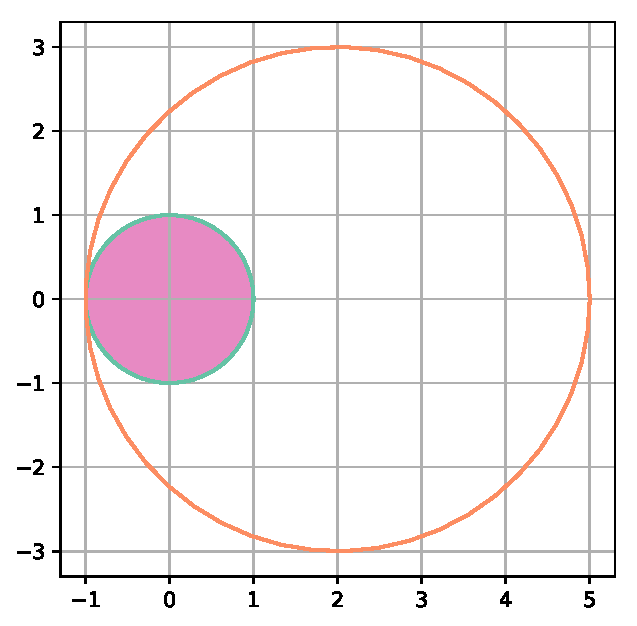
\includegraphics[width=0.31\textwidth]{figs/lens_2_1_3}
\par\end{centering}
\label{fig:cylindrical-integration-region}}\hfill{}\subfloat[Standard lens integration region]{\begin{centering}
\includegraphics[width=0.31\textwidth]{figs/lens_2\lyxdot 5_1_2\lyxdot 5}
\par\end{centering}
\label{fig:lens-integration-region}}\hfill{}\subfloat[Non-standard lens integration region]{\begin{centering}
\includegraphics[width=0.31\textwidth]{figs/lens_2_1_2\lyxdot 5}
\par\end{centering}
\label{fig:irregular-integration-region}}
\par\end{centering}
\caption{Meshless integration regions in transformed coordinates}

\label{fig:integration-regions}
\end{figure}


\subsubsection{Cartesian regions }

Integration quadratures such as the Gauss-Legendre quadrature used
here are often given over the range $\left[-1,1\right]$. To calculate
the integration ordinates, the geometry is mapped onto simple Cartesian
regions. In one dimension, to convert from $x\in\left[x_{1},x_{2}\right]$
to $\xi\in\left[-1,1\right]$, the mapping\begin{subequations}
\begin{equation}
x\left(\xi\right)=\frac{1-\xi}{2}x_{1}+\frac{1+\xi}{2}x_{2}
\end{equation}
is applied. The differential length for the mapping is then
\begin{equation}
dx=\frac{x_{2}-x_{1}}{2}d\xi.
\end{equation}
\end{subequations}After the change of variables, a one-dimensional
integral over the Cartesian region $x\in\left[x_{1},x_{2}\right]$
has the form \begin{subequations}\label{eq:cartesian-2d-integral}
\begin{align}
\int_{x_{1}}^{x_{2}}f\left(x\right)dx & =\frac{x_{2}-x_{1}}{2}\int_{-1}^{1}f\left(x\left(\xi\right)\right)d\xi\nonumber \\
 & =\frac{x_{2}-x_{1}}{2}\sum_{i}c_{i}f\left(x\left(\xi_{i}\right)\right)\nonumber \\
 & =\sum_{i}C_{i}f\left(X_{i}\right),
\end{align}
where $\xi_{i}$ are the original integration ordinates in $\xi\in\left[-1,1\right]$
and $c_{i}$ are the original integration weights. The modified integration
ordinates and weights are then 
\begin{gather}
X_{i}=x\left(\xi_{i}\right),\\
C_{i}=\frac{x_{2}-x_{1}}{2}c_{i}.
\end{gather}
\end{subequations}

For a Cartesian region in 2D, the conversion from $x\in\left[x_{1},x_{2}\right]$
and $y\in\left[y_{1},y_{2}\right]$ to $\xi\in\left[-1,1\right]$
and $\eta\in\left[-1,1\right]$ follows the same process, using the
mappings\begin{subequations}
\begin{gather}
x\left(\xi\right)=\frac{1-\xi}{2}x_{1}+\frac{1+\xi}{2}x_{2},\\
y\left(\eta\right)=\frac{1-\eta}{2}y_{1}+\frac{1-\eta}{2}y_{2}.
\end{gather}
The differentials are independent due to the orthogonality of the
coordinate system,
\begin{gather}
dx=\frac{x_{2}-x_{1}}{2}d\xi,\\
dy=\frac{y_{2}-y_{1}}{2}d\eta,
\end{gather}
\end{subequations}and a two-dimensional integral over this region
becomes
\begin{align}
\int_{x_{1}}^{x_{2}}\int_{y_{1}}^{y_{2}}f\left(x,y\right)dxdy & =\frac{x_{2}-x_{1}}{2}\frac{y_{2}-y_{1}}{2}\int_{-1}^{1}\int_{-1}^{1}f\left(x\left(\xi\right),y\left(\eta\right)\right)d\xi d\eta\nonumber \\
 & =\frac{x_{2}-x_{1}}{2}\frac{y_{2}-y_{1}}{2}\sum_{i,j}c_{i}^{x}c_{j}^{x}f\left(x\left(\xi_{i}\right),y\left(\eta_{j}\right)\right).
\end{align}
The modified integration ordinates and weights can be calculated similarly
to those in Eq. (\ref{eq:cartesian-2d-integral}). 

\subsubsection{Cylinder}

In cylindrical coordinates, the integrals are first mapped from cylindrical
to Cartesian coordinates, and then finally to a local coordinate system.
The mapping from radial coordinates with $r\in\left[r_{1},r_{2}\right]$
and $\theta\in\left[\theta_{1},\theta_{2}\right]$ to Cartesian coordinates
is\begin{subequations}
\begin{gather}
x\left(r,\theta\right)=x_{0}+r\cos\theta,\\
y\left(r,\theta\right)=y_{0}+r\sin\theta,
\end{gather}
\end{subequations}where $\bm{x}_{0}=\left(x_{0},\ y_{0}\right)$
is the location of the center of the cylinder. The integral is then
converted to local coordinates by the transformations\begin{subequations}
\begin{gather*}
r=\frac{1-\xi}{2}r_{1}+\frac{1+\xi}{2}r_{2},\\
\theta=\frac{1-\eta}{2}\theta_{1}+\frac{1+\eta}{2}\theta_{2},
\end{gather*}
for $\xi\in\left[-1,1\right]$ and $\eta\in\left[-1,1\right]$. As
the coordinate system is orthogonal as for the Cartesian case, the
differentials are independent,
\begin{gather*}
dr=\frac{r_{2}-r_{1}}{2}d\xi,\\
d\theta=\frac{\theta_{2}-\theta_{1}}{2}d\eta.
\end{gather*}
\end{subequations}The integrals after being converted to local coordinates
are
\begin{align}
\int_{\theta_{1}}^{\theta_{2}}\int_{r_{1}}^{r_{2}}f\left(x\left(r,\theta\right),y\left(r,\theta\right)\right)rdrd\theta & =\frac{r_{2}-r_{1}}{2}\frac{\theta_{2}-\theta_{1}}{2}\int_{-1}^{1}\int_{-1}^{1}f\left(x\left(r\left(\xi\right),\theta\left(\eta\right)\right),y\left(r\left(\xi\right),\theta\left(\eta\right)\right)\right)r\left(\xi\right)d\xi d\eta\nonumber \\
 & =\frac{r_{2}-r_{1}}{2}\frac{\theta_{2}-\theta_{1}}{2}\sum_{i,j}f\left(x\left(r\left(\xi_{i}\right),\theta\left(\eta_{j}\right)\right),y\left(r\left(\xi_{i}\right),\theta\left(\eta_{j}\right)\right)\right)r\left(\xi_{i}\right).
\end{align}
This quadrature region and integration points are shown in Figs. \ref{fig:cylindrical-integration-region}
and \ref{fig:integration-cylindrical}, respectively. 

\begin{figure}[!b]
\begin{centering}
\subfloat[Standard lens integration quadrature]{\begin{centering}
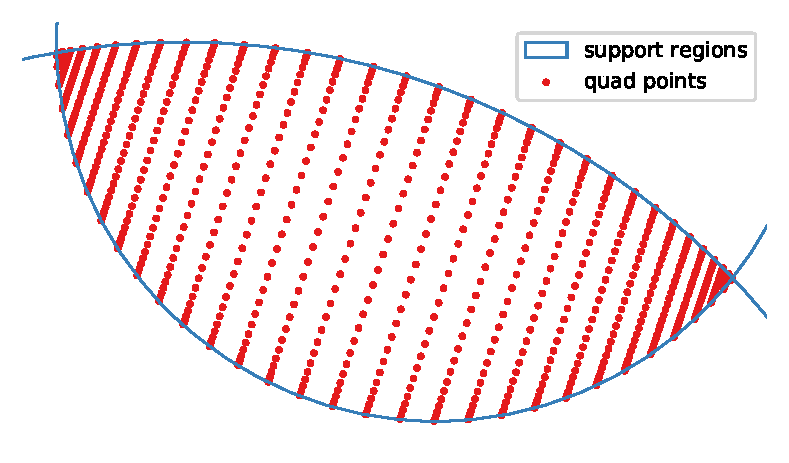
\includegraphics[width=0.47\textwidth]{figs/quad_lens2}
\par\end{centering}
\label{fig:integration-lens-standard}}\hfill{}\subfloat[Quadrature near a boundary]{\begin{centering}
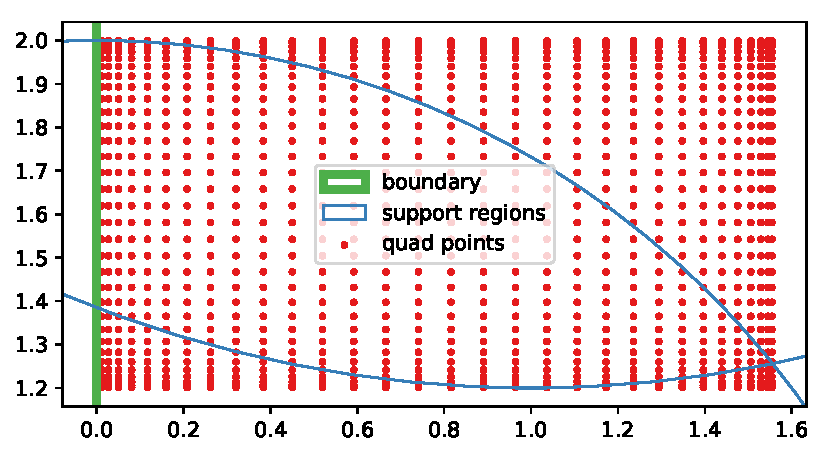
\includegraphics[width=0.47\textwidth]{figs/quad_lens4}
\par\end{centering}
\label{fig:integration-lens-boundary}}
\par\end{centering}
\begin{centering}
\subfloat[Non-standard lens integration region]{\begin{centering}
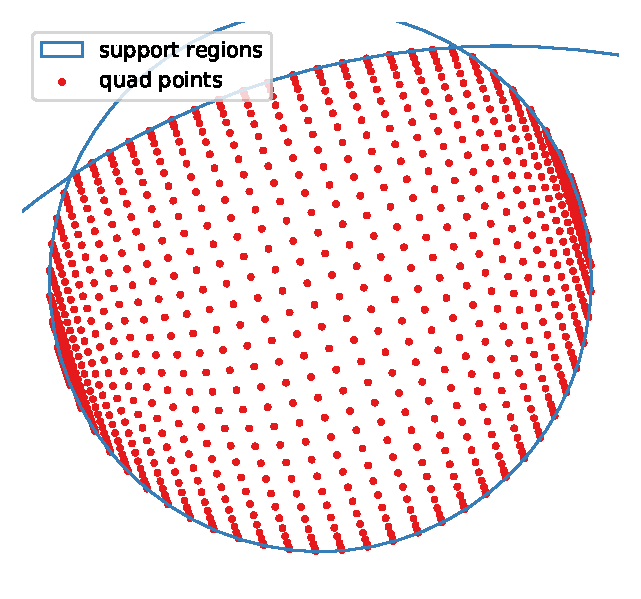
\includegraphics[width=0.47\textwidth]{figs/quad_lens3}
\par\end{centering}
\label{fig:integration-lens-nonstandard}}\hfill{}\subfloat[Cylindrical integration region]{\begin{centering}
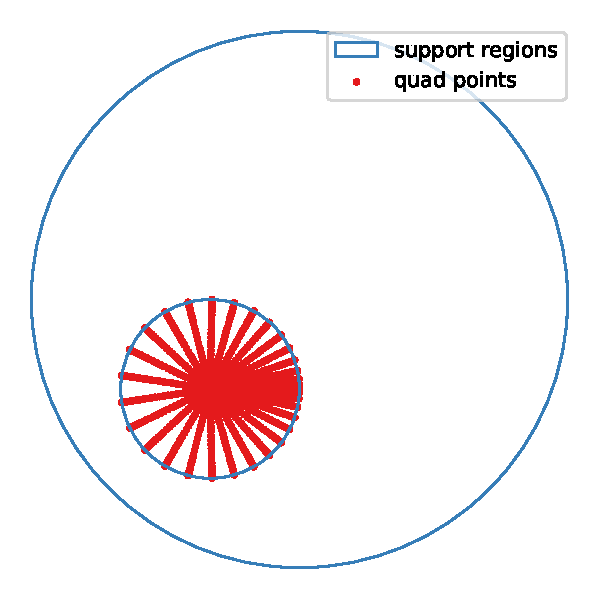
\includegraphics[width=0.47\textwidth]{figs/quad_lens5}
\par\end{centering}
\label{fig:integration-cylindrical}}
\par\end{centering}
\caption{Quadratures for meshless integration}

\label{fig:integration-quadratures}
\end{figure}


\subsubsection{Standard lens\label{subsec:standard-lens}}

For the simple lens pictured in Figs. \ref{fig:lens-integration-region}
and \ref{fig:integration-lens-standard} the two intercepts of the
circles are not past the center of either circle. The coordinate system
is rotated so both radii are located at the same point on the $y$
axis and then translated so that one of the circles is located at
the origin. In this coordinate system, all integrals appear similar
to the one pictured in Fig. \ref{fig:lens-integration-region}. 

This transformation from the Cartesian coordinates $x,y$ to simplified
coordinates $\bar{x},\bar{y}$ has the form \begin{subequations}
\begin{equation}
\left[\begin{array}{c}
\bar{x}\\
\bar{y}
\end{array}\right]=\left[\begin{array}{c}
x_{1}\\
y_{1}
\end{array}\right]+\frac{1}{d}\left[\begin{array}{cc}
\Delta x & -\Delta y\\
\Delta y & \Delta x
\end{array}\right]\left[\begin{array}{c}
x\\
y
\end{array}\right],
\end{equation}
with the distances
\begin{gather}
\Delta x=x_{2}-x_{1},\\
\Delta y=y_{2}-y_{1},\\
d=\sqrt{\Delta x^{2}+\Delta y^{2}}.
\end{gather}
\end{subequations}In this coordinate system, the equations for each
circular support region can be written\begin{subequations}
\begin{gather}
\bar{x}^{2}+\bar{y}^{2}=r_{1}^{2},\\
\left(\bar{x}-d\right)^{2}+\bar{y}^{2}=r_{2}^{2},
\end{gather}
\end{subequations}where the radii of the circles (which remain unchanged
in this coordinate system) are $r_{1}$ and $r_{2}$. The two intercepts
of these circles are located at the points $\left(\bar{x}_{int},\ \bar{y}_{int}\right)$
and $\left(\bar{x}_{int},\ -\bar{y}_{int}\right)$, with \begin{subequations}
\begin{gather}
\bar{x}_{int}=\frac{d^{2}+r_{1}^{2}-r_{2}^{2}}{2d},\\
\bar{y}_{int}=\frac{\sqrt{2d^{2}\left(r_{1}^{2}+r_{2}^{2}\right)-\left(r_{1}^{2}-r_{2}^{2}\right)^{2}-d^{4}}}{2d}.
\end{gather}
\end{subequations}The integration limits in the $\bar{x}$ dimension
are variable with respect to $\bar{y}$,\begin{subequations}
\begin{gather}
\bar{x}_{min}\left(\bar{y}\right)=d-\sqrt{r_{2}^{2}-\bar{y}^{2}},\\
\bar{x}_{max}\left(\bar{y}\right)=\sqrt{r_{1}^{2}-\bar{y}^{2}},
\end{gather}
\end{subequations}while the integration limits in the $\bar{y}$
dimension go from $-\bar{y}_{int}$ to $\bar{y}_{int}$. 

The conversion of the integral from Cartesian to simplified coordinates
has a Jacobian determinant of one,
\begin{equation}
J_{\left(x,y\right)\to\left(\bar{x},\bar{y}\right)}=\left|\begin{array}{cc}
\dfrac{dx}{d\bar{x}} & \dfrac{dx}{d\bar{x}}\\
\dfrac{dy}{d\bar{x}} & \dfrac{dy}{d\bar{y}}
\end{array}\right|=1,
\end{equation}
which means the integral can be transformed to the simplified coordinates
as
\begin{equation}
\int_{V}f\left(x,y\right)dV=\int_{-\bar{y}_{int}}^{\bar{y}_{int}}\int_{\bar{x}_{min}\left(\bar{y}\right)}^{\bar{x}_{max}\left(\bar{y}\right)}f\left(x\left(\bar{x},\bar{y}\right),y\left(\bar{x},\bar{y}\right)\right)d\bar{x}d\bar{y}.
\end{equation}

This integral is transformed a second time from the simplified coordinate
system into a standard coordinate system $\xi\in\left[-1,1\right]$
and $\eta\in\left[-1,1\right]$ using \begin{subequations}
\begin{gather}
\bar{x}=\frac{\bar{x}_{max}\left(\bar{y}\left(\eta\right)\right)-\bar{x}_{min}\left(\bar{y}\left(\eta\right)\right)}{2}\xi+\frac{\bar{x}_{max}\left(\bar{y}\left(\eta\right)\right)+\bar{x}_{min}\left(\bar{y}\left(\eta\right)\right)}{2},\\
\bar{y}=\bar{y}_{int}\eta.
\end{gather}
\end{subequations}Unlike the first transformation, the Jacobian determinant
for this transformation is not equal to a constant,
\begin{equation}
J_{\left(\bar{x},\bar{y}\right)\to\left(\xi,\eta\right)}=\left|\begin{array}{cc}
\dfrac{d\bar{x}}{d\xi} & \dfrac{d\bar{x}}{d\eta}\\
\dfrac{d\bar{y}}{d\xi} & \dfrac{d\bar{y}}{d\eta}
\end{array}\right|=\left(\frac{\bar{x}_{max}\left(\bar{y}\right)-\bar{x}_{min}\left(\bar{y}\right)}{2}\right)\bar{y}_{int}.
\end{equation}
This Jacobian is used to map the integral to the local coordinates,
\begin{equation}
\int_{V}f\left(x,y\right)dV=\int_{-1}^{1}\int_{-1}^{1}f\left(x\left(\bar{x},\bar{y}\right),y\left(\bar{x},\bar{y}\right)\right)\left(\frac{\bar{x}_{max}\left(\bar{y}\right)-\bar{x}_{min}\left(\bar{y}\right)}{2}\right)\bar{y}_{int}d\xi d\eta.\label{eq:lens-integral}
\end{equation}
For simplicity, the dependencies of $\bar{x}$ and $\bar{y}$ on $\xi$
and $\eta$ have been suppressed. The conversion of this continuous
integral to a numerical quadrature follows the same procedure as in
past sections. 

\subsubsection{Non-standard lens\label{subsec:non-standard-lens}}

The second type of lens uses the same coordinate system and intercepts
as in Sec. \ref{subsec:standard-lens}. The difference is that the
$\bar{x}$ intercept is past the center of one of the circles, as
shown in Fig. \ref{fig:irregular-integration-region}. Assuming that
the first circle with $r_{1}$ has the smaller radius $\left(r_{1}<r_{2}\right)$
and that the intercept is past the center of the first circle, the
integration is of the same form as for the standard lens but with
$\bar{x}$ limits of 
\begin{gather*}
\bar{x}_{min}\left(\bar{y}\right)=\begin{cases}
d-\sqrt{r_{2}^{2}-\bar{y}^{2}}, & \left|\bar{y}\right|\leq\bar{y}_{int},\\
-\sqrt{r_{1}^{2}-\bar{y}^{2}}, & \text{otherwise},
\end{cases}\\
\bar{x}_{max}\left(\bar{y}\right)=\sqrt{r_{1}^{2}-\bar{y}^{2}}.
\end{gather*}
If $r_{2}>r_{1}$, then the definitions reverse,
\begin{gather*}
\bar{x}_{min}\left(\bar{y}\right)=d-\sqrt{r_{2}^{2}-\bar{y}^{2}}\\
\bar{x}_{max}\left(\bar{y}\right)=\begin{cases}
\sqrt{r_{1}^{2}-\bar{y}^{2}}, & \left|\bar{y}\right|\leq\bar{y}_{int},\\
d+\sqrt{r_{2}^{2}-\bar{y}^{2}}, & \text{otherwise},
\end{cases}.
\end{gather*}
The integral can be calculated using Eq. (\ref{eq:lens-integral})
with these $\bar{x}$ limits and the same $\bar{y}\in\left(-\bar{y}_{int},\ \bar{y}_{int}\right)$
limits as before. 

\subsubsection{Methodology}

For the integrals only involving weight functions and not basis functions,
as in Eq. (\ref{eq:source-integrals}), the region of integration
is cylindrical except near boundaries, where the Cartesian quadrature
is used instead. For integrals involving both basis and weight functions,
one of the lens quadratures or the cylindrical quadrature are used
away from boundaries and the Cartesian quadrature is used for lens
regions that intersect boundaries. One benefit of the meshless integration
approach is that unlike the background mesh integration in Sec. \ref{subsec:background-mesh-integration},
the meshless integration is independent for each weight function.
This means that the integration of weight functions can be done in
parallel with no special considerations for shared data. 

Due to the simpler parallelization and independent nature of the meshless
integration, the implementation is in some ways simpler than the background
mesh integration. The issue with the meshless integration is that
much of the computational cost of the integration is evaluation of
the weight and basis functions, which is particularly expensive for
the \gls{mls} functions (Sec. \ref{subsec:moving-least-squares}).
The basis functions each intersect with many weight functions, some
of which have support regions that overlap. This means that the quadrature
sets for the basis and weight functions overlap many times over. In
addition, the weight function values must be calculated for each individual
basis function integral separately as the quadrature points differ.
Some of this cost could be defrayed by doing the integrals of the
basis functions over the entire weight function region, but this would
reduce the accuracy of the quadrature. 

\subsection{Background mesh integration\label{subsec:background-mesh-integration}}

In contrast to the meshless integration method, the background integration
mesh method uses non-overlapping quadratures to increase integration
efficiency. The integration regions no longer conform to the exact
integration domains as in the meshless method, but as the cost of
the method is lower per area integrated, more quadrature points can
be used to compensate. Because the basis and weight functions chosen
in Sec. \ref{subsec:meshless-functions} go to zero at the edge of
their support region, there are no discontinuities in the functions
that need special treatment when using a background integration mesh.
The cross sections, however, do add discontinuities that require consideration. 

To perform the integration using a background mesh, the problem is
overlaid with a Cartesian mesh to create cells for the volume integration
and faces along the boundaries for the surface integration. This background
mesh is agnostic to the problem geometry and is only used for the
integration step, not for the solution of the transport equations.
Algorithm \ref{alg:background-integration} describes the background
integration procedure. In summary, the integration is performed by
choosing a quadrature for each integration cell, evaluating all needed
data at each quadrature point and then adding the contribution of
each quadrature point to the global integral. The quadrature inside
of each Cartesian cell is an outer product Gaussian quadrature, e.g.
for a function $f\left(x,y,z\right)$, 
\begin{equation}
\int_{\text{cell}}f\left(x,y,z\right)dV=\sum_{i,j,k}c_{i}^{x}c_{j}^{y}c_{k}^{z}f\left(x_{i},y_{j},z_{k}\right),\label{eq:cartesian-cell-quad}
\end{equation}
where the one-dimensional quadrature integration ordinates are $x_{i}$,
$y_{i}$ and $z_{k}$ with corresponding weights of $c_{i}^{x}$,
$c_{j}^{y}$ and $c_{k}^{z}$. This integral is done using the same
transformations as the Cartesian quadrature in Eq. (\ref{eq:cartesian-2d-integral})
applied to the 1D, 2D or 3D volume integral. 

\begin{algorithm}[!tb]
\begin{algorithmic}[1] 
\State{\textbf{initialize} all integrals to zero}
\ForEach{background cell or face (region $i$)}
\State{\textbf{create} a quadrature that integrates region $i$}
\State{\textbf{find} the basis and weight functions that intersect with region $i$}
\ForEach{quadrature point $j$}
\State{\textbf{evaluate} each basis and weight function and their derivatives at point $j$}
\State{\textbf{find} the values of the cross sections and sources at point $j$}
\ForEach{required integral}
\State{\textbf{add} the contribution of this quadrature point to the global integral}
\EndFor
\EndFor
\EndFor
\end{algorithmic}\caption{Procedure for integration using a background mesh}
\label{alg:background-integration}
\end{algorithm}

The integration quadrature for each cell can be adaptively chosen
for problems in which radii of the intersecting functions differ significantly.
For the adaptive quadrature, a minimum number of integration ordinates
across the basis or weight function $N_{rad}$ is specified. The number
of integration ordinates for the cell along each dimension is chosen
using the basis or weight function with the smallest radius $r$ inside
the cell as
\begin{equation}
N_{d}=\frac{\ell_{d}}{r}N_{rad},\label{eq:adaptive-quadrature}
\end{equation}
where $\ell_{d}$ is the length of the cell in that dimension, for
instance the side length of a Cartesian cell, which defines an outer
product quadrature with $\prod_{d}N_{d}$ total ordinates.

The integration is done independently for each cell and face, which
allows for parallelization of the integration step (see Sec. \ref{subsec:parallelization}).
Each processor needs access to the basis and weight function data
for each integration cell assigned to it. Once the integration has
been performed for the cells assigned to each processor, the integrals
are reduced to sum the contributions of each integration cell to the
overall integrals of the basis and weight functions.

\subsection{Integration verification against benchmark problem\label{subsec:integration-verification}}

To verify the integration methods, three configurations of basis and
weight function intersections (including those described in Sec. \ref{subsec:meshless-integration})
are considered and the integrals are performed individually to high
precision using Mathematica \cite{wolfram-mathematica}. The positions
of the basis and weight functions for each case are shown in Fig.
\ref{fig:benchmark-integration}. The basis and weight functions use
the Wendland 11 \gls{rbf}. The integrals $\overline{i}_{bw;i,j}^{V}$
and $\overline{\bm{I}}_{\nabla b\nabla w;i,j}$ from Eq. (\ref{eq:basis-weight-integrals})
are compared to the benchmark values by calculating the total $L_{2}$
error,
\begin{equation}
\epsilon_{L_{2}}=\frac{1}{N_{\text{weight}}}\sum_{j}\sqrt{\frac{\sum_{i}\left(\bar{i}_{bw;i,j}-\bar{i}_{bw;i,j}^{\text{benchmark}}\right)^{2}}{\sum_{i}\left(\bar{i}_{bw;i,j}^{\text{benchmark}}\right)^{2}}}.\label{eq:l2-integration}
\end{equation}
For the derivative integrals, the values summed inside the square
root term include the derivatives. 

\begin{figure}[!b]
\begin{centering}
\subfloat[First configuration]{\begin{centering}
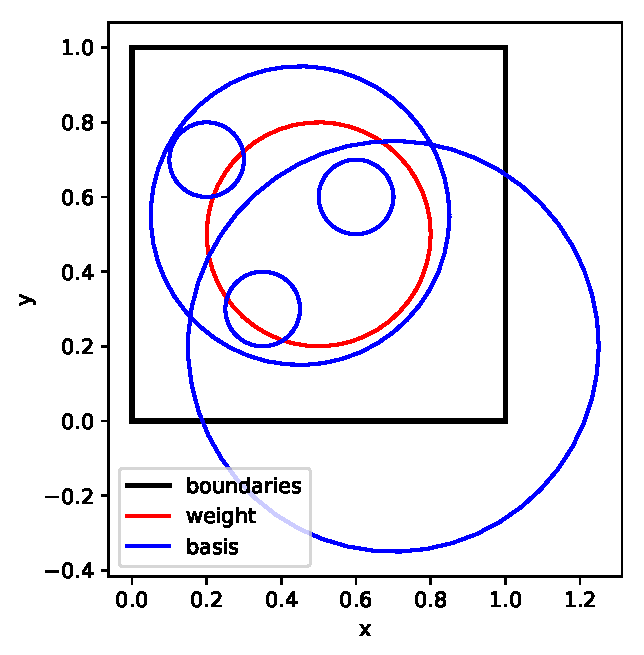
\includegraphics[width=0.31\textwidth]{figs/weight_test_1}
\par\end{centering}
}\hfill{}\subfloat[Second configuration]{\begin{centering}
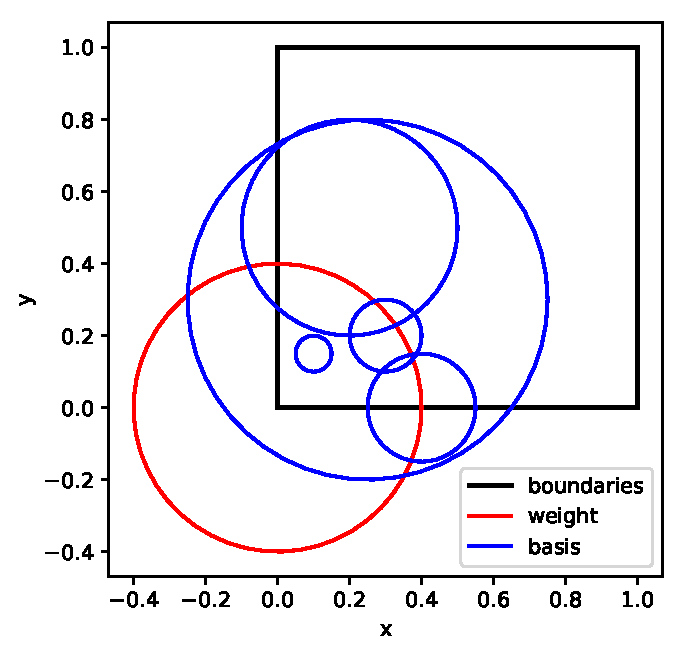
\includegraphics[width=0.31\textwidth]{figs/weight_test_2}
\par\end{centering}
}\hfill{}\subfloat[Third configuration]{\begin{centering}
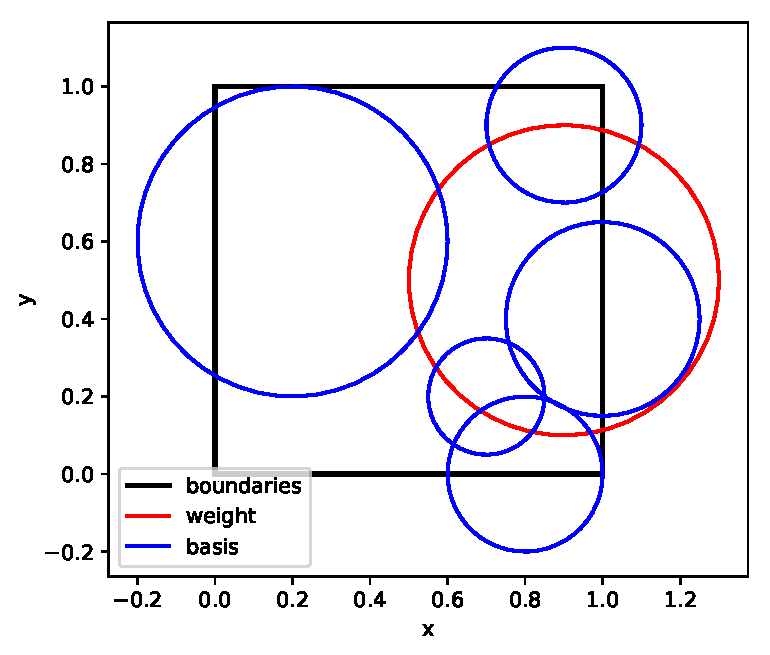
\includegraphics[width=0.31\textwidth]{figs/weight_test_3}
\par\end{centering}
}
\par\end{centering}
\caption{Basis and weight function configurations for verification of numerical
integration against benchmark}

\label{fig:benchmark-integration}
\end{figure}

For the meshless integration method, between $4^{2}$ and $2048^{2}$
quadrature points are used to integrate each basis and weight function
pair. For the background integration method, quadratures with the
same range of values are used in each of the $10^{2}$ background
cells. This results in a higher number of points inside each integration
region for the background mesh, which is balanced by the increased
accuracy of a specialized quadrature for the meshless integration
method. Due to the small number of weight and basis functions, the
two quadratures aren't directly compared in terms of computational
cost in this section. 

The convergence results for the two integration methods are shown
in Fig. \ref{fig:benchmark-integration-convergence}. Both integration
methods show approximately fourth-order convergence as the number
of integration points in one of the dimensions increases. Once the
number of integration ordinates reaches about $1024^{2}$ for either
method, the relative $L_{2}$ error for the $\bar{i}_{bw}$ integrals
is below $10^{-12}$. For problems with more integration ordinates,
the error increases again, likely because of numerical roundoff. The
derivative integrals $\bar{i}_{\nabla b\nabla w}$ converge at around
the same rate and by $2048^{2}$ ordinates, the results from both
methods have a relative error below $10^{-12}$. 

\begin{figure}[!tb]
\begin{centering}
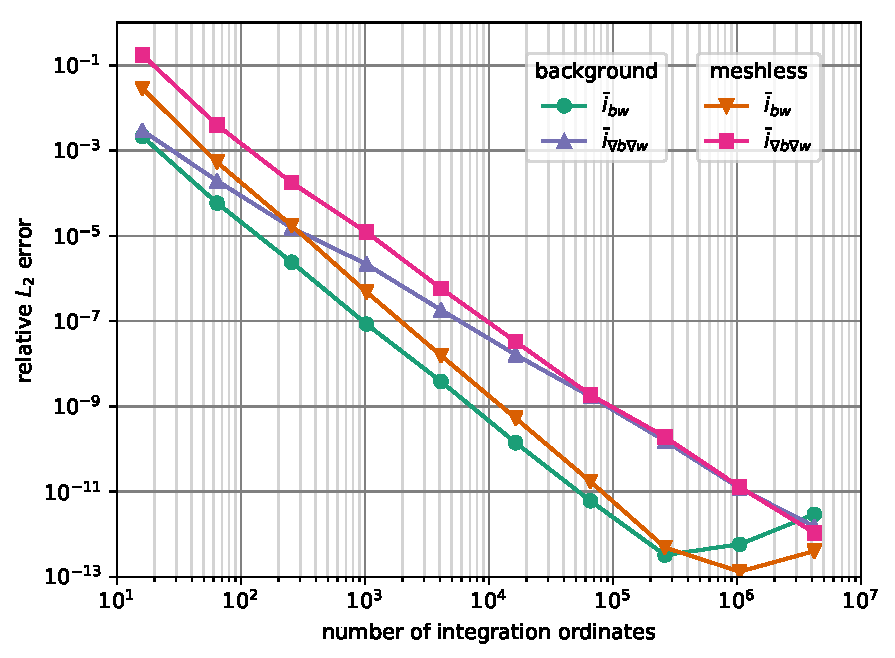
\includegraphics[width=0.47\textwidth]{figs/analytic_integration_convergence}
\par\end{centering}
\caption{Convergence for the benchmark integration problem for meshless and
background mesh integration}
\label{fig:benchmark-integration-convergence}
\end{figure}


\subsection{Comparison of integration methods\label{subsec:comparison-of-integration}}

For comparison of the basis and weight function integration methods,
a set of 100 compact Gaussian functions {[}Eq. (\ref{eq:compact-gaussian}){]}
with a dimensionless cutoff distance of $R=5$ are created in 1D,
2D and 3D. The centers of these functions are placed at random in
the problem domain, $\bm{x}\in\left[-2,2\right]$. Figure \ref{fig:integration-comparison-geometry}
shows the point configurations for the 2D and 3D problems. The randomized
points result in some clusters of points and some points without close
neighbors. This means that the calculated radii vary over more than
an order of magnitude, similar to a realistic problem with small features
that need to be resolved. 

\begin{figure}[!tb]
\begin{centering}
\subfloat[2D]{\begin{centering}
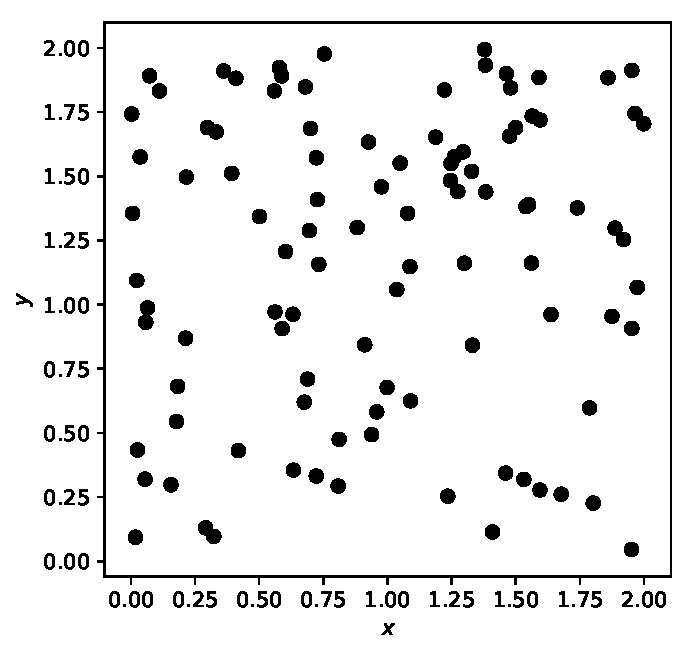
\includegraphics[width=0.4\textwidth]{figs/integration_comparison_fig_2d}
\par\end{centering}
}\hfill{}\subfloat[3D]{\begin{centering}
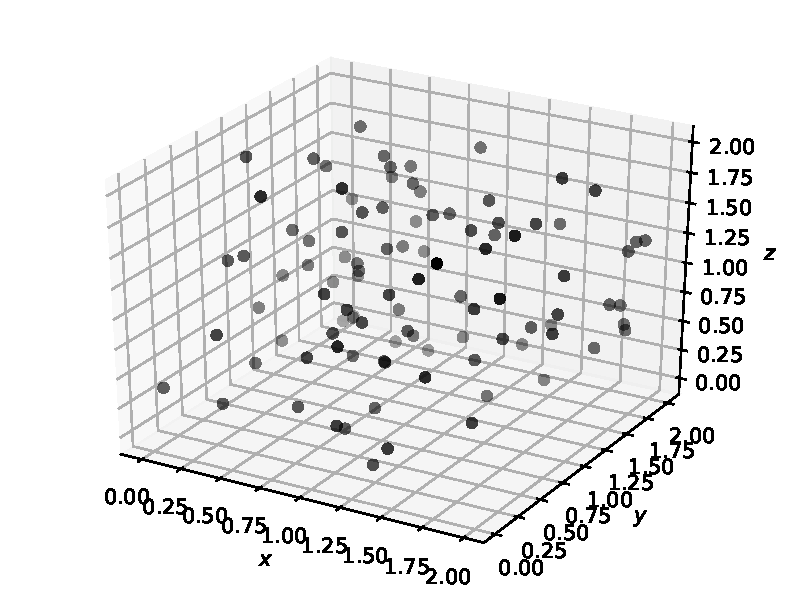
\includegraphics[width=0.54\textwidth]{figs/integration_comparison_fig_3d}
\par\end{centering}
}
\par\end{centering}
\caption{Randomized positions of centers for comparison of integration methods}

\label{fig:integration-comparison-geometry}
\end{figure}

For the results with a background mesh, 100 (1D and 2D) or 125 (3D)
background cells are placed with even spacing. The number of integration
ordinates in a cell for the adaptive method is initially set to $8^{d}$
(for the dimension $d$) before potentially being modified according
to Eq. (\ref{eq:adaptive-quadrature}). The number of ordinates for
the background mesh without adaptive integration refers to the number
in each integration cell, which multiplied by the number of cells
is the total number of integration ordinates. For the meshless integration,
the number of integration ordinates is fixed for each integral. 

A benchmark solution is calculated using the adaptive integration
method with a high number of integration ordinates ($4096$ in 1D,
$1024^{2}$ in 2D and $128^{3}$ in 3D) and the result for the other
methods is compared to this solution. The same $L_{2}$ error as in
Eq. (\ref{eq:l2-integration}) is used to find the errors in the integrals
of the basis and weight functions and their derivatives with respect
to the benchmark solution. To compare the relative performance of
the methods, the error is presented as a function of the local number
of integration ordinates and separately as a function of the total
number of basis and weight function evaluations, which represents
a large part of the integration cost. 

The results for the $L_{2}$ error in 1D, 2D and 3D are shown in Fig.
\ref{fig:integration-comparison}. All three methods show at least
eighth-order convergence with the integration ordinate spacing. The
convergence rate is highest for the adaptive case. Both the adaptive
and the meshless integration methods scale the quadrature to the size
of the radii, which improves the convergence rate. In 1D, the relative
error converges to $10^{-13}$ for both the integrals and the derivatives.
In 2D and 3D, the relative error converges to $10^{-11}$ and $10^{-10}$,
respectively. The adaptive integration method achieves the best results
for a given number of function evaluations. The meshless integration
requires around an order of magnitude more function evaluations to
achieve the same error as the background mesh methods. Due to the
simple Wendland 11 functions used and the additional complexity of
the background integration, the computational time is similar in this
problem for a given error for the meshless and background integration
methods. 

\begin{figure}[!p]
\begin{centering}
\subfloat[Convergence with local number of integration ordinates, 1D]{\begin{centering}
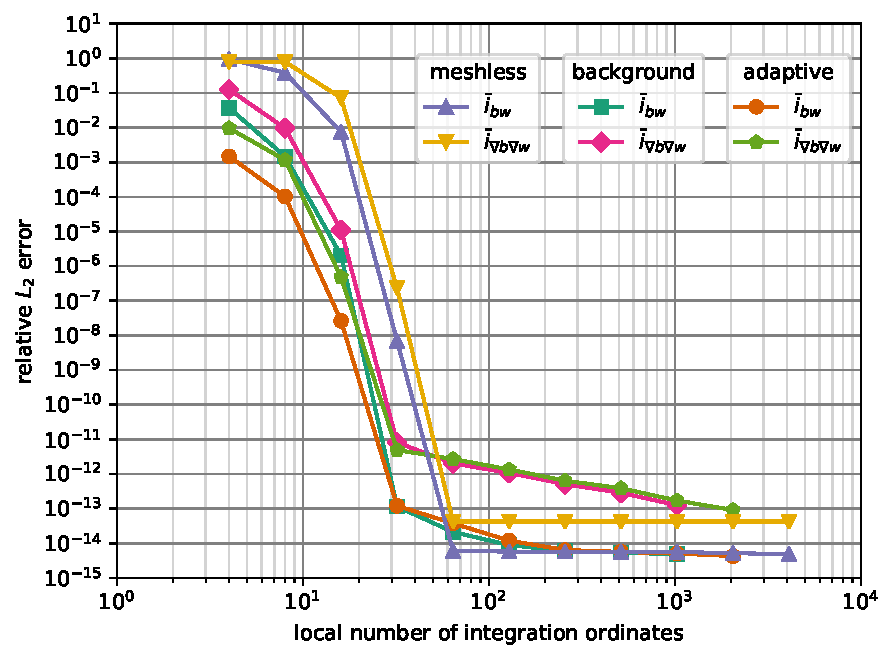
\includegraphics[width=0.47\textwidth]{figs/integration_comparison_1d}
\par\end{centering}
\label{fig:integration-comparison-1d}}\hfill{}\subfloat[Convergence with total number of function evaluations, 1D]{\begin{centering}
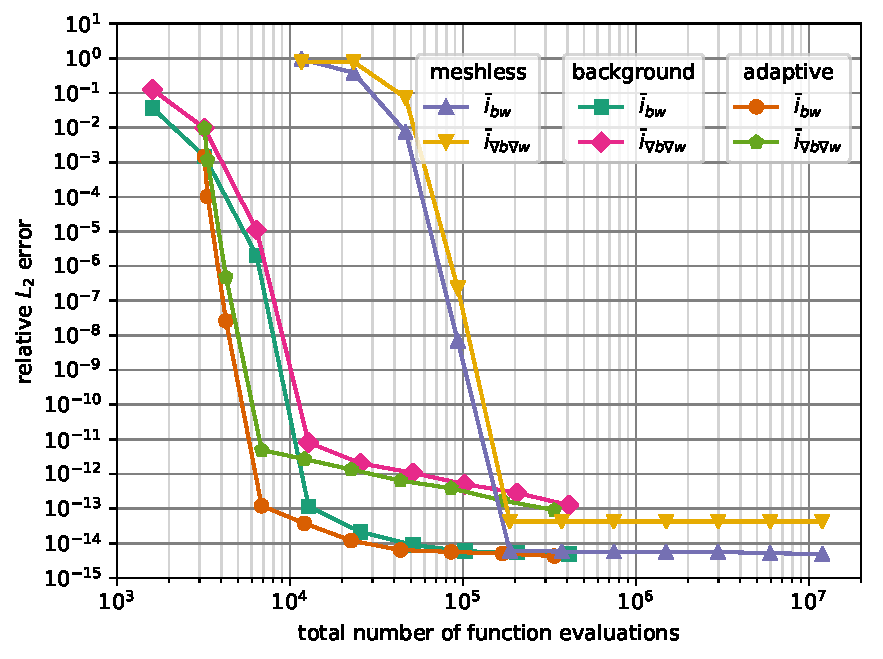
\includegraphics[width=0.47\textwidth]{figs/integration_comparison_tot_1d}
\par\end{centering}
\label{fig:integration-comparison-fom-1d}}
\par\end{centering}
\begin{centering}
\subfloat[Convergence with local number of integration ordinates, 2D]{\begin{centering}
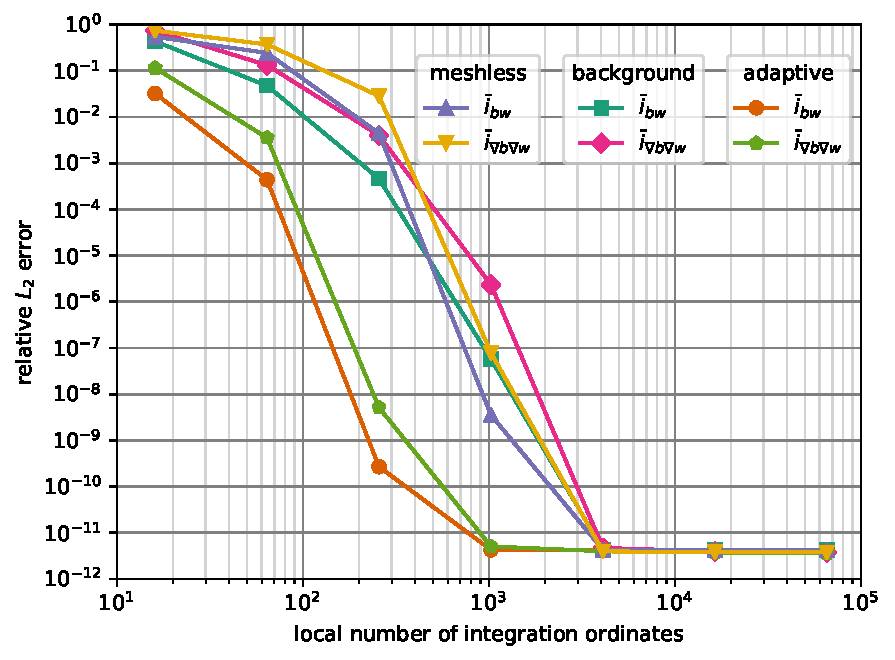
\includegraphics[width=0.47\textwidth]{figs/integration_comparison_2d}
\par\end{centering}
\label{fig:integration-comparison-2d}}\hfill{}\subfloat[Convergence with total number of function evaluations, 2D]{\begin{centering}
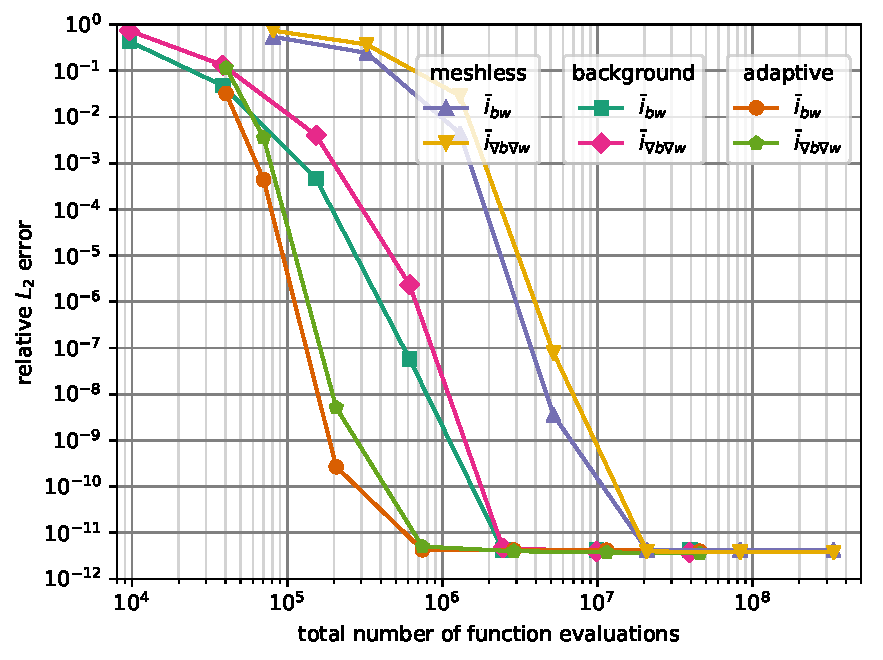
\includegraphics[width=0.47\textwidth]{figs/integration_comparison_tot_2d}
\par\end{centering}
\label{fig:integration-comparison-fom-2d}}
\par\end{centering}
\begin{centering}
\subfloat[Convergence with local number of integration ordinates, 3D]{\begin{centering}
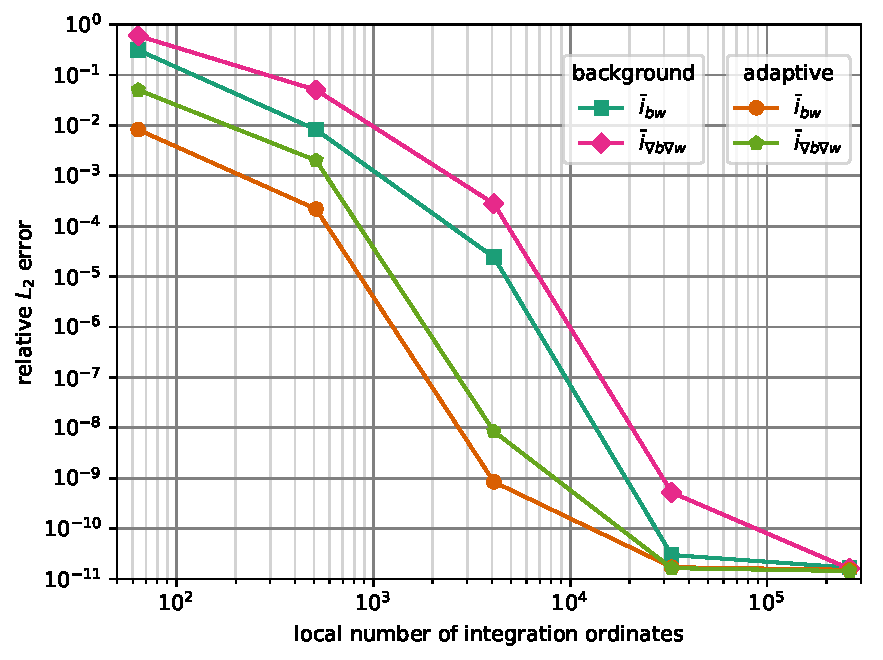
\includegraphics[width=0.47\textwidth]{figs/integration_comparison_3d}
\par\end{centering}
\label{fig:integration-comparison-3d}}\hfill{}\subfloat[Convergence with total number of function evaluations, 3D]{\begin{centering}
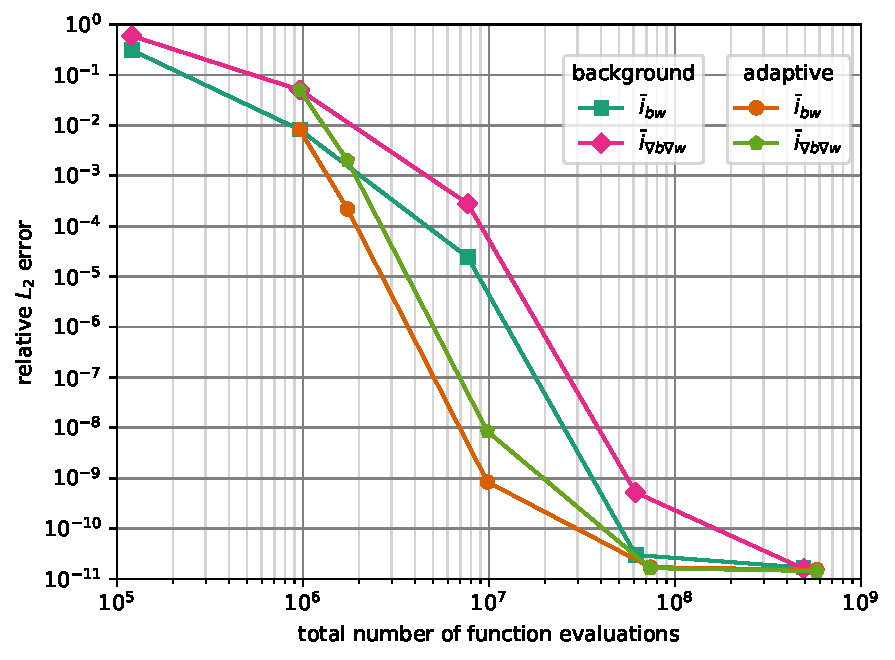
\includegraphics[width=0.47\textwidth]{figs/integration_comparison_tot_3d}
\par\end{centering}
\label{fig:integration-comparison-fom-3d}}
\par\end{centering}
\caption{Comparison of integration methods, convergence to benchmark solution}

\label{fig:integration-comparison}
\end{figure}

While the performance of the meshless integration in this problem
is not significantly worse than the background integration, that is
not the case for a problem with \gls{mls} functions. The compact
Gaussian functions are inexpensive to evaluate, whereas the \gls{mls}
functions are not. As all the basis and weight functions are evaluated
at the same quadrature points, all the values at a single quadrature
point as described in Sec. \ref{subsec:moving-least-squares} can
be calculated simultaneously. For the meshless method, the weight
and basis function do not share a common quadrature, which multiplies
the cost of integration for \gls{mls} functions by 20 to 70 times,
depending on the dimension of the problem and the radii of the basis
and weight functions. As such, applying the meshless integration method
to \gls{mls} functions for a large number of integration ordinates
is not practical and the meshless integration is not used for the
results in the following chapters. In addition, the benefits of a
quadrature that exactly conforms to the integration domain are not
as important in problems with large discontinuities, which are best
integrated by a quadrature with a large number of evaluation points
as opposed to a quadrature that very accurately integrates a certain
class of smooth equations.

\subsection{VERA pincell integration problem\label{subsec:vera-pincell-integration}}

\begin{figure}[!b]
\begin{centering}
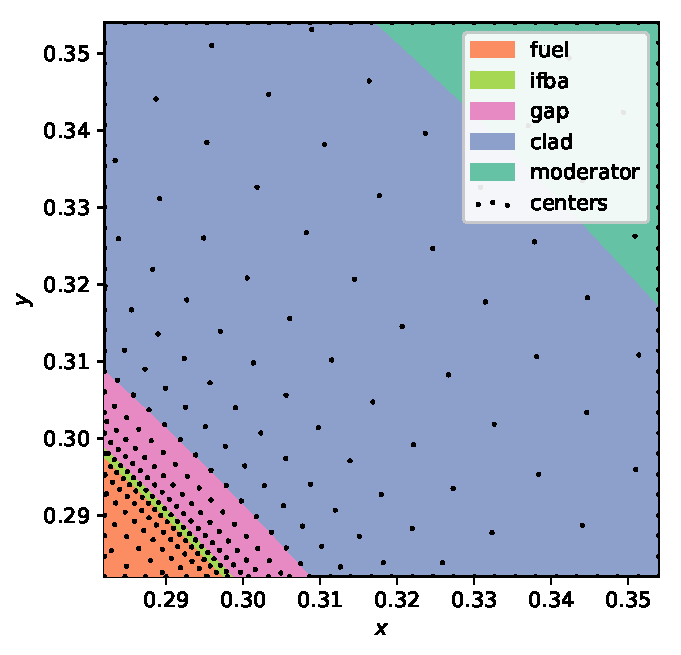
\includegraphics[width=0.47\textwidth]{figs/vera_integration_geometry}
\par\end{centering}
\caption{VERA pincell integration geometry}
\label{fig:vera-integration-geometry}
\end{figure}

This final integration test investigates the use of \gls{mls} functions
functions in a heterogeneous medium. For reasons explained at the
end of Sec. \ref{subsec:comparison-of-integration}, only the background
integration mesh methods are applied here. The geometry for the heterogeneous
test is a small section of the \gls{vera} 1E geometry from Sec. \ref{subsec:vera}.
As shown in Fig. \ref{fig:vera-integration-geometry}, the section
under consideration ($0.282\leq\bm{x}\leq0.354$) is near the fuel
boundary and includes all five materials from the original \gls{vera}
problem. The cross sections vary over several orders of magnitude,
which makes the material integration particularly difficult. The points
are preferentially placed near the \gls{ifba} region where the discontinuities
in the cross sections are largest and the gradient in the transport
solution is largest. For reference, this is a subset of the 34085-point
set used for the \gls{vera} 1E problem (Sec. \ref{subsec:vera})
with additional points added around the boundaries. Additional points
are added along the boundaries to ensure coverage of the functions
throughout the problem. This is essential for the calculation of the
\gls{mls} functions, which requires that several functions have nonzero
values at every point in the domain (see Sec. \ref{subsec:moving-least-squares}). 

The radii of the basis and weight functions are calculated using Alg.
\ref{alg:radius-calculation} with eight neighbors. The radii range
between 0.0015 near the \gls{ifba} region to 0.015 near the clad-moderator
boundary. These disparate radii make the integration difficult, as
a Cartesian background mesh with a constant number of integration
points includes more integration points for basis and weight functions
with larger radii. When using a background mesh without an adaptive
number of integration ordinates, the same number of ordinates per
unit area are used for both the functions with large radii and the
functions with small radii. When the enough integration points have
been added to resolve the integrals of the smallest functions, the
integrals of the largest functions may have more points than is required
for accurate integration. 

The subdomain of the \gls{vera} 1E problem considered here has a
length 17.5 times smaller than the length of the full problem, and
an area of 306.25 times smaller. The goal of this integration study
is not to simply get a good integration result, but to get a good
integration result in a timely manner. The number of background cells
chosen is $20^{2}$, which would be equivalent to a background mesh
with $350^{2}$ cells for the full pincell problem. This results in
$4N$ total ordinates across the radii of the largest functions and
$0.4N$ ordinates across the radii of the smallest functions, where
$N^{2}$ is the number of integration ordinates in the Cartesian product
quadrature. The number of ordinates is varied from $4^{2}$ to $256^{2}$
for the background integration without an adaptive quadrature. For
the adaptive quadrature, the number of ordinates required across each
weight function radius {[}Eq. (\ref{eq:adaptive-quadrature}){]} is
varied between $4$ and $256$, with a baseline number of integration
ordinates in a cell of $4^{2}$. The benchmark calculation is performed
using $512^{2}$ as the baseline number of integration ordinates and
$512$ as the minimum number of integration ordinates across each
radius. 

Figure \ref{fig:vera-integration-results} shows the error of the
integrals with an increasing number of integration ordinates. For
the number of integration points considered, the basis and weight
function integrals converge to $10^{-7}$ relative error and the basis
and weight derivative integrals converge to $10^{-6}$ relative error.
To achieve a similar error, the adaptive integration technique requires
between 2 and 10 times fewer global integration points than the method
without adaptive integration. 

\begin{figure}[!p]
\begin{centering}
\subfloat[Basis and weight function integrals by local number of integration
ordinates]{\begin{centering}
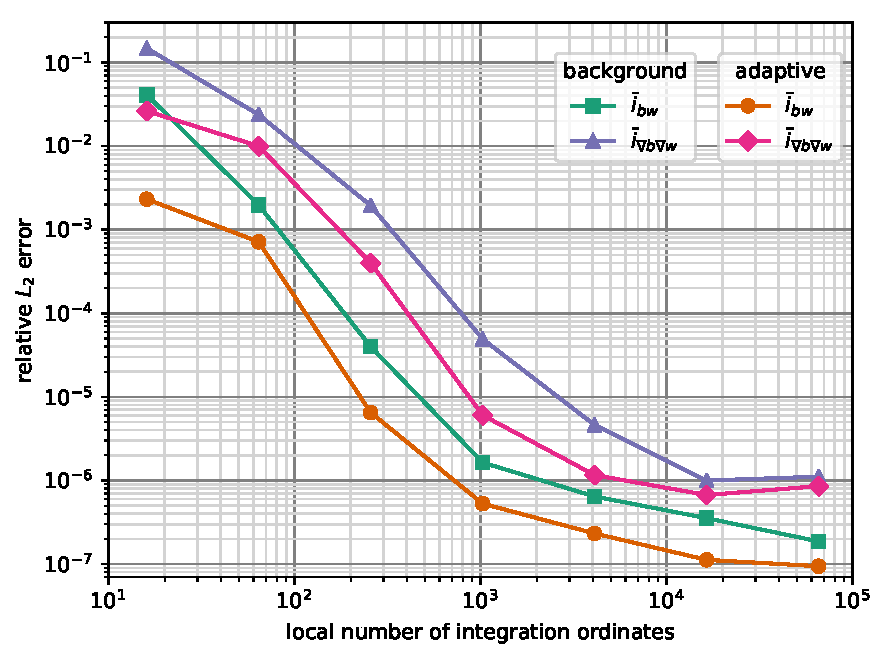
\includegraphics[width=0.47\textwidth]{figs/vera_integration_conv}
\par\end{centering}
\label{fig:vera-integration-bw-local}}\hfill{}\subfloat[Basis and weight function integral $L_{2}$ error by global number
of integration ordinates]{\begin{centering}
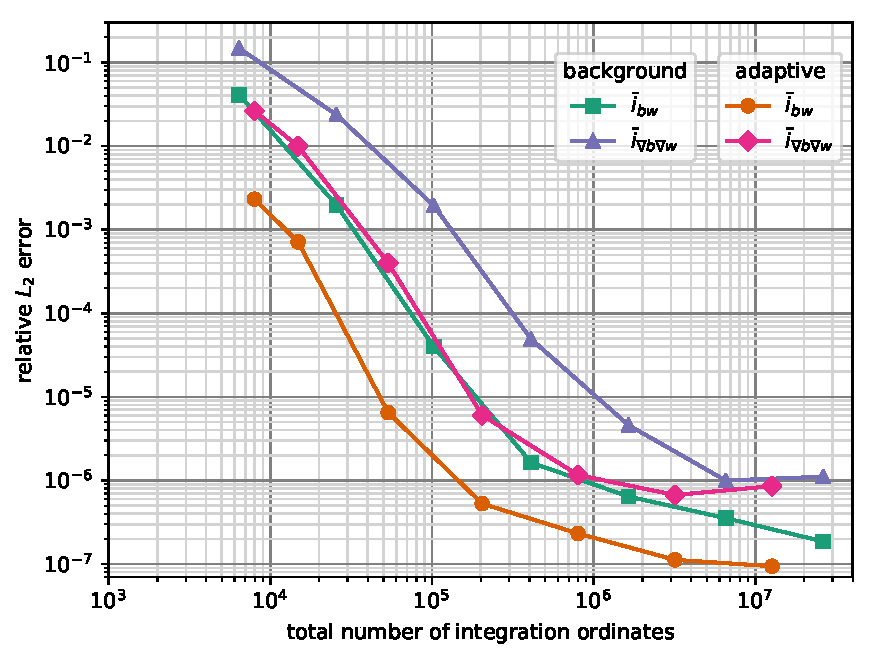
\includegraphics[width=0.47\textwidth]{figs/vera_integration_conv_tot}
\par\end{centering}
\label{fig:vera-integration-bw-global}}
\par\end{centering}
\begin{centering}
\subfloat[Cross section integral $L_{2}$ error by local number of integration
ordinates]{\begin{centering}
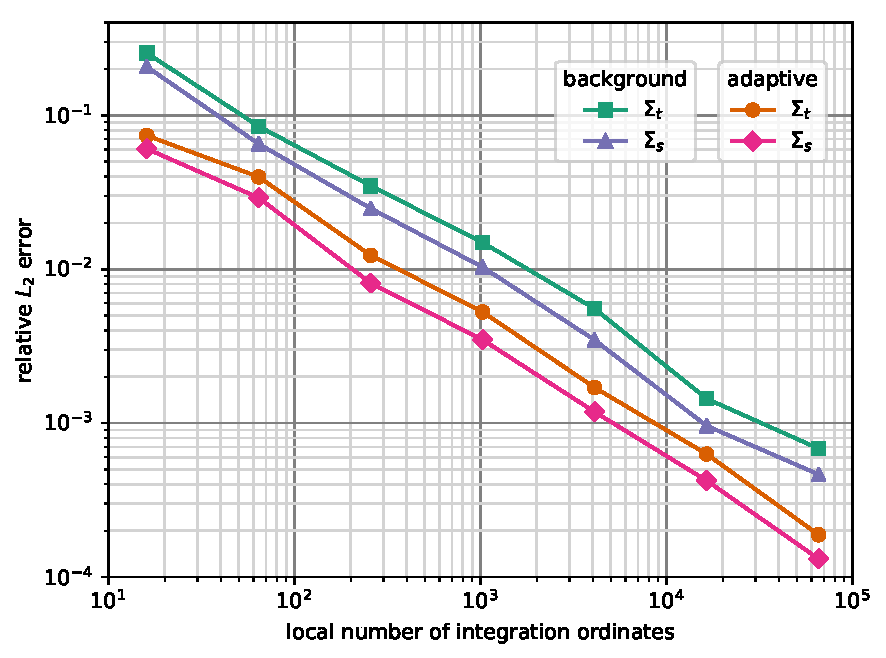
\includegraphics[width=0.47\textwidth]{figs/vera_integration_conv_sig}
\par\end{centering}
\label{fig:vera-integration-sig-local}}\hfill{}\subfloat[Cross section integral $L_{2}$ error by global number of integration
ordinates]{\begin{centering}
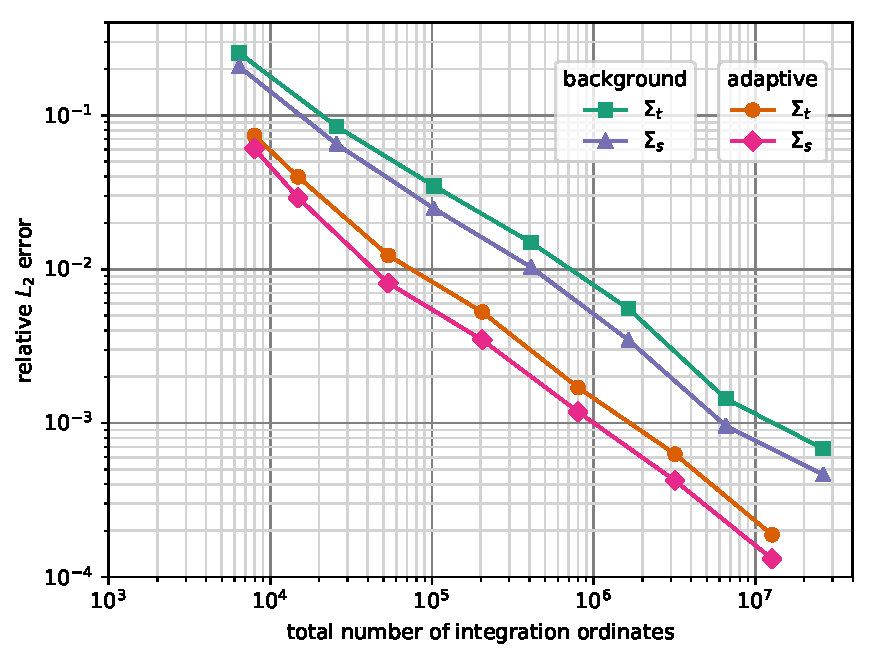
\includegraphics[width=0.47\textwidth]{figs/vera_integration_conv_tot_sig}
\par\end{centering}
\label{fig:vera-integration-sig-global}}
\par\end{centering}
\caption{Convergence of VERA pincell integration to benchmark solution}

\label{fig:vera-integration-results}
\end{figure}

\begin{figure}[!p]
\begin{centering}
\subfloat[Relative error in the integral $\int_{V}b_{i}w_{j}dV$]{\begin{centering}
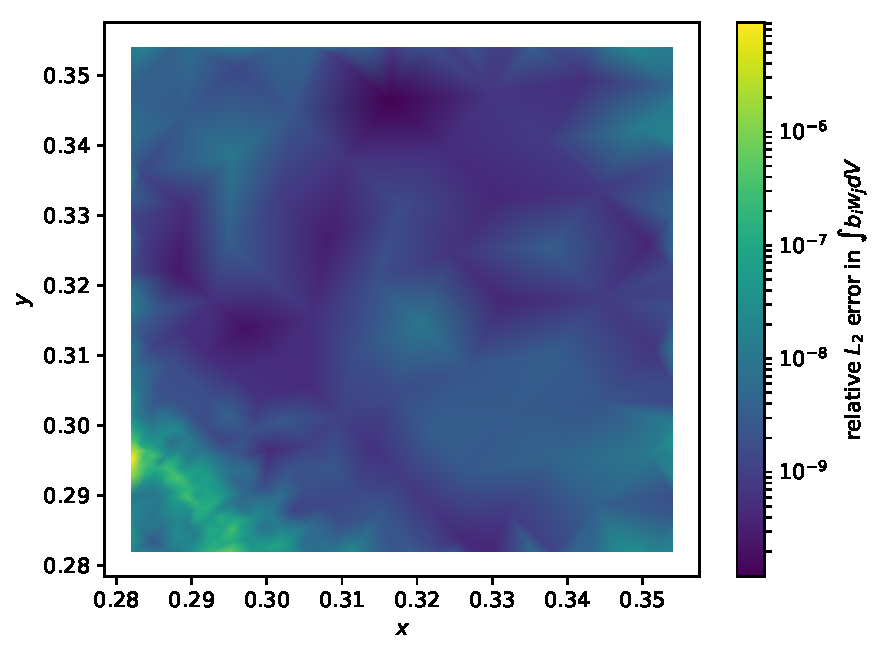
\includegraphics[width=0.47\textwidth]{figs/vera_integration_integral}
\par\end{centering}
}\hfill{}\subfloat[Relative error in the integral $\int_{V}\Sigma_{t}b_{i}w_{j}dV$]{\begin{centering}
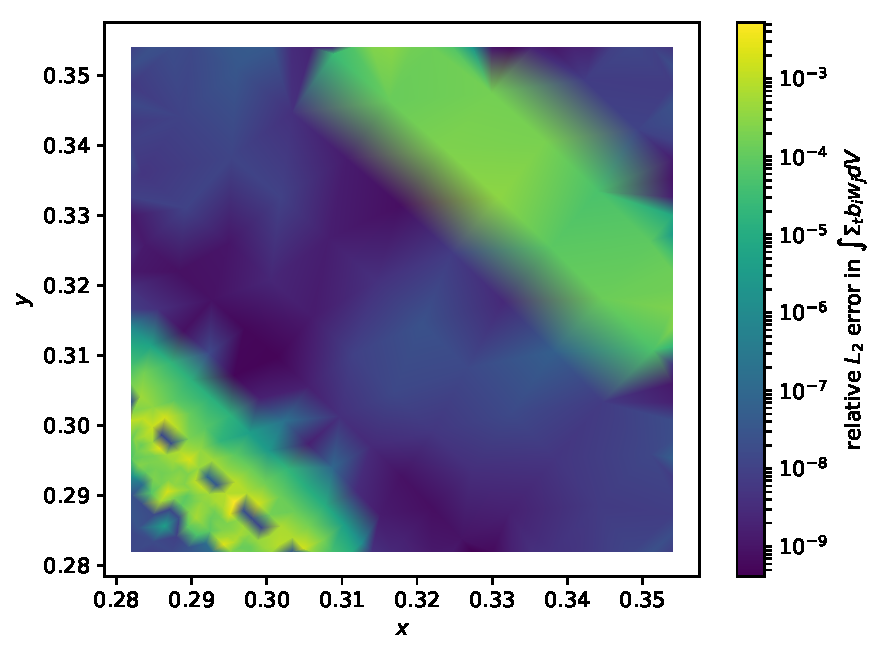
\includegraphics[width=0.47\textwidth]{figs/vera_integration_sigma-t}
\par\end{centering}
}
\par\end{centering}
\caption{VERA pincell integration error for adaptive problem with $256^{2}$
local integration ordinates}

\label{fig:vera-integration-error}
\end{figure}

The integrals of the basis and weight functions over the total and
scattering cross sections {[}Eqs. (\ref{eq:sigma_t-full}) and (\ref{eq:sigma_s-full}){]}
converge less quickly than the \gls{mls} function integrals due to
the discontinuities in the integration domain. The chosen discretization
has a higher density of basis and weight functions near the largest
of the discontinuities. The adaptive integration puts more integration
points near these functions due to their small radii, which also increases
the accuracy of integration for the discontinuities. Compared to the
background mesh integration without adaptivity, the adaptive method
again requires far fewer global integration ordinates (an order of
magnitude for the cases with the most ordinates) to achieve similar
errors for the cross section integrals and has a higher rate of convergence
to the benchmark result. For the highest number of integration ordinates
considered, the relative $L_{2}$ error of the adaptive integration
is around $10^{-4}$ for both the total and cross section integrals. 

Figure \ref{fig:vera-integration-error} shows the relative $L_{2}$
error for the adaptive integration with 256 ordinates as a function
of position for the basis and weight function integrals and the cross
section integrals. The basis and weight functions with the highest
relative integration error are those with the smallest radii. The
cross section integrals error is effectively identical to the basis
and weight function integral error in regions with constant cross
section values. The integration is least accurate near the fuel boundary,
where there are three materials within 10 \textgreek{m}m. The error
also increases near the material discontinuity at the clad-moderator
boundary. 

One large difference between the Gaussian functions integrated in
Sec. \ref{subsec:comparison-of-integration} and the linear \gls{mls}
functions integrated here is that the former have a simple polynomial
series expansion, whereas the latter do not. The Gauss-Legendre tensor
product quadrature is designed to integrate polynomials with high
accuracy and as such works well for functions such as the Gaussian
and the Wendland functions that can be represented as polynomials.
The integrals of linear \gls{mls} functions require more integration
points than either of these to be accurate. 

The \gls{mls} functions have good properties for solving the transport
equation, including partition of unity and the ability to turn a relatively
sparse set of \gls{rbf}s into a basis that can accurately represent
polynomials, but they are costly to evaluate and difficult to integrate
accurately. The background mesh with an adaptive quadrature provides
predictable results for the integration of \gls{mls} functions of
disparate sizes at a reasonable level of computational cost. 

\cleardoublepage{}

\sectionspacing

\section{Verification by the method of manufactured solutions\label{sec:method-of-manufactured}}

In this section, the method of manufactured solutions (\gls{mms})
is used to verify that the \gls{mlpg} equations are accurately solved
using the discretizations in Chapter \ref{sec:transport-discretization}.
This includes derivation of the method of manufactured solutions for
the transport equations (Sec. \ref{subsec:manufactured-equations});
presentation of the two test problems (Sec. \ref{subsec:manufactured-problems});
and optimization of the solution for the radii of the basis and weight
functions and the \gls{supg} parameters (Sec. \ref{subsec:manufactured-results}). 

\subsection{The method of manufactured solutions\label{subsec:manufactured-equations}}

The process of verification by the \gls{mms} begins with a manufactured
solution to the equation, which for the \gls{mlpg} equations derived
in Chapter \ref{sec:transport-discretization} is the moments of the
angular flux, $\phi_{\ell,g}^{m}\left(\bm{x}\right)$. The manufactured
solution, which is denoted here by $\Phi_{\ell,g}^{m}\left(\bm{x}\right)$,
is inserted into the original equation to analytically calculate the
moments of the internal source, $Q_{\ell,g}^{m}\left(\bm{x}\right)$,
and the boundary source, $\psi_{n,g}^{inc}\left(\bm{x}\right)$. A
simulation is performed using these sources to calculate a numerical
solution to the problem. If the code is working correctly, the numerical
solution matches the manufactured solution. 

To calculate the expected internal source for the transport equation,
the internal source is expanded using spherical harmonics {[}as in
Eq. (\ref{eq:source-expansion}){]}. The spherical harmonics moments
are orthogonal, meaning that 
\begin{equation}
\int_{4\pi}Y_{\ell}^{m}\left(\bm{\Omega}\right)Y_{\ell'}^{m'}\left(\bm{\Omega}\right)d\Omega=\frac{4\pi}{2\ell+1}\delta_{\ell,\ell'}\delta_{m,m'},
\end{equation}
where $\delta_{a,b}$ is the Kronecker delta function from Eq. (\ref{eq:delta-function}).
For example, multiplying the internal source term in the transport
equation by $Y_{\ell'}^{m'}$ and integrating over the unit sphere
results in the equation
\begin{equation}
\int_{4\pi}Y_{\ell'}^{m'}\left[\sum_{\ell=0}^{L}\frac{2\ell+1}{4\pi}\sum_{m=-\ell}^{\ell}Y_{\ell}^{m}Q_{\ell,g}^{m}\right]d\Omega=\begin{cases}
Q_{\ell,g}, & \ell'=\ell'\text{ and }m'=m',\\
0, & \text{otherwise},
\end{cases}
\end{equation}
which isolates the moments of the internal source. To calculate the
manufactured internal source, the manufactured flux is inserted into
the multigroup transport equation {[}Eq. (\ref{eq:multigroup}){]}
with the steady-state approximation. This equation with the known
manufactured solution $\Phi_{\ell,g}^{m}$ is multiplied by $Y_{\ell'}^{m'}$
and integrated over all directions. Using the orthogonality property,
the resulting transport equation can be solved for $Q_{\ell,g}$,
\begin{align}
Q_{\ell,g}^{m} & =\int_{4\pi}Y_{\ell}^{m}\Biggl[\bm{\Omega}\cdot\bm{\nabla}\Psi_{g}+\Sigma_{t;g}\Psi_{g}\nonumber \\
 & \qquad\qquad\qquad\left.-\sum_{\ell'=0}^{\infty}\frac{2\ell'+1}{4\pi}\sum_{m'=-\ell}^{\ell}Y_{\ell'}^{m'}\sum_{g'=1}^{G}\Sigma_{s;\ell',g'\to g}\Phi_{\ell',g'}^{m'}-\frac{\chi_{g}}{4\pi}\sum_{g'=1}^{G}\nu_{g'}\Sigma_{f;g'}\Phi_{0,g'}^{0}d\Omega\right].
\end{align}
Replacing the manufactured angular flux $\Psi_{g}$ by a spherical
harmonics expansion in terms of $\Phi_{\ell,g}^{m}$ and using orthogonality
to perform the integration for the scattering and fission terms, the
equation simplifies to 
\begin{align}
Q_{\ell,g} & =\sum_{\ell'=0}^{\infty}\sum_{m'=-\ell}^{\ell}\left(\frac{2\ell'+1}{4\pi}\int_{4\pi}\bm{\Omega}Y_{\ell}^{m}Y_{\ell'}^{m'}d\Omega\right)\cdot\bm{\nabla}\Phi_{\ell',g}^{m'}+\Sigma_{t;g}\Phi_{\ell,g}^{m}\nonumber \\
 & \qquad-\sum_{g'=1}^{G}\Sigma_{s;\ell,g'\to g}\Phi_{\ell,g'}^{m}-\delta_{\ell,0}\chi_{g}\sum_{g'=1}^{G}\nu_{g'}\Sigma_{f;g'\to g}\Phi_{\ell,g'}^{m}.\label{eq:manufactured-internal}
\end{align}
Due to the $\bm{\Omega}$ term inside the remaining angular integral,
if the manufactured solution has spherical harmonics moments of maximum
degree $L$, the calculated source $Q_{\ell,g}^{m}$ has nonzero values
of one spherical harmonic degree higher, or $L+1$. This integral,
which is of the form 
\begin{equation}
\frac{2\ell'+1}{4\pi}\int_{4\pi}Y_{1}^{m''}Y_{\ell'}^{m'}Y_{\ell}^{m}d\Omega
\end{equation}
for $m''=-1,0,1$, can be performed analytically using Clebsch-Gordon
coefficients. For simplicity, this integral is performed numerically
for the problems in Sec. \ref{subsec:manufactured-problems} using
a Gauss-Legendre quadrature with 256 ordinates in 1D or an \gls{ldfe}
quadrature with 16384 or 32768 ordinates in 2D or 3D, respectively. 

The boundary source for the manufactured equations is set to the value
of the desired source, or 
\begin{equation}
\psi_{n,g}^{inc}=\sum_{\ell=0}^{L}\frac{2\ell+1}{4\pi}\sum_{m=-\ell}^{\ell}Y_{\ell}^{m}\left(\bm{\Omega}_{n}\right)\Phi_{\ell,g}^{m},\label{eq:manufactured-boundary}
\end{equation}
and reflection is disabled. If the boundary integration is done correctly,
the value at the boundary is equal the desired solution.

The process of testing the manufactured solution includes:
\begin{enumerate}
\item Defining the problem geometry, including cross sections;
\item Initializing the internal source as defined by Eq. (\ref{eq:manufactured-internal})
and the boundary source defined by Eq. (\ref{eq:manufactured-boundary});
\item Performing the integration (for the weak form) or evaluation (for
the strong form) of the internal source and the boundary source using
these cross sections and sources;
\item Solving the steady-state transport equation; and
\item Calculating the error of the numerical solution with respect to the
initial manufactured solution.
\end{enumerate}
The \gls{mms} allows benchmarking of problems that would be difficult
to solve using established codes. For instance, in Sec. \ref{subsec:manufactured-problems},
the transport equation is solved with continuously-variable cross
sections, which as discussed in Sec. \ref{subsec:difficulties-in-neutron}
is not a common capability for a neutron transport code. Another benefit
of the \gls{mms} is that it removes errors (in deterministic calculations)
or uncertainties (in Monte Carlo calculations) from the benchmark
solution. 

\subsection{Introduction to continuous and discontinuous manufactured problems\label{subsec:manufactured-problems}}

The two manufactured problems considered here are a problem with piecewise
constant cross sections and a problem with continuous, sinusoidal
cross sections. The manufactured solutions and cross sections are
defined in three dimensions. For two dimensions, the solutions and
cross sections are evaluated at $z=0$. For both problems, the basis
and weight function centers are placed on the nodes of an equally-spaced
Cartesian grid with an equal number of points in each dimension, $N_{x}=N_{y}=N_{z}$.
The problems use 256 and 512 angular quadrature ordinates in 2D and
3D, respectively. The number of points, the number of neighbors in
the radius calculation, the Wendland function {[}Eqs. (\ref{eq:wendland}){]}
and the value of the \gls{supg} parameter $\tau$ are all varied
to find optimal values that converge appropriately and retain good
conditioning for the $\mathcal{L}^{-1}$ operation. For each permutation
of parameters, the flux $\phi_{\ell,g}^{m}$ is calculated and compared
to the initial manufactured flux, $\Phi_{\ell,g}^{m}$. The relative
$L_{1}$ integral error over the entire problem domain $V$,
\begin{equation}
\left(L_{1}\text{ integral error}\right)_{g}=\frac{\int_{V}\left|\phi_{0,g}^{0}-\Phi_{0,g}^{0}\right|dV}{\int_{V}\Phi_{0,g}^{0}dV},\label{eq:l1-error-manufactured}
\end{equation}
is then calculated numerically using a Gauss-Legendre outer product
quadrature to measure convergence and compare between parameters. 

The first problem, which has two energy groups and a domain of $-0.01\leq x,y,z\leq0.01$,
uses the cross sections in Table \ref{tab:vera1e-xs} from the \gls{vera}
1E problem as described in Sec. \ref{subsec:vera}. The cross sections
are piecewise constant and depend only on the distance from the origin,
$r=\left\Vert \bm{x}\right\Vert $, making the cross sections cylindrically
symmetric in two dimensions and spherically symmetric in three dimensions.
The three cross sections used include the fuel cross sections from
$0.0\leq r\leq0.0045$, the \gls{ifba} (integral fuel burnable absorber)
cross sections from $0.0045<x\leq0.0055$ and the gap cross sections
for $0.0055<r$. These cross sections represent a fissionable isotope,
a strong thermal absorber and a near-vacuum. The solution to this
problem is also chosen to have cylindrical or spherical symmetry,
\begin{equation}
\Phi_{\ell,g}^{m}\left(\bm{x}\right)=f_{\ell,g}^{m}\exp\left(a_{g}\left\Vert \bm{x}\right\Vert \right)\left[1+b_{g}\exp\left(c_{g}\left[\left\Vert \bm{x}\right\Vert +d_{g}\right]^{2}\right)\right],\label{eq:manufactured-radial-sol}
\end{equation}
with the constants from Table \ref{tab:manufactured-piecewise-sol}.
Figure \ref{fig:manufactured-radial-solution} shows the solution
in two dimensions for the fast and thermal groups. The thermal group
solution has a sharp valley in the \gls{ifba} region, which tests
the effect of sharp gradients on the number of neighbors and choice
of Wendland function. 

\begin{table}[!tb]
\caption{Manufactured solution coefficients for radially symmetric problem
{[}see Eq. (\ref{eq:manufactured-radial-sol}){]}}

\centering{}%
\begin{tabular}{|c|c|c|c|c|c|c|c|c|}
\hline 
Group & $f_{0,g}^{0}$ & $f_{1,g}^{-1}$ & $f_{1,g}^{0}$ & $f_{1,g}^{1}$ & $a_{g}$ & $b_{g}$ & $c_{g}$ & $d_{g}$\tabularnewline
\hline 
\hline 
1 & 1.0 & 0.0 & 0.1 & -0.05 & -10.0 & -0.1 & -$10^{5}$ & -0.0075\tabularnewline
\hline 
2 & 2.0 & 0.0 & -0.2 & 0.1 & 10.0 & -0.2 & $10^{7}$ & -0.005\tabularnewline
\hline 
\end{tabular}\label{tab:manufactured-piecewise-sol}
\end{table}

\begin{figure}[!tb]
\begin{centering}
\subfloat[Fast energy group]{\begin{centering}
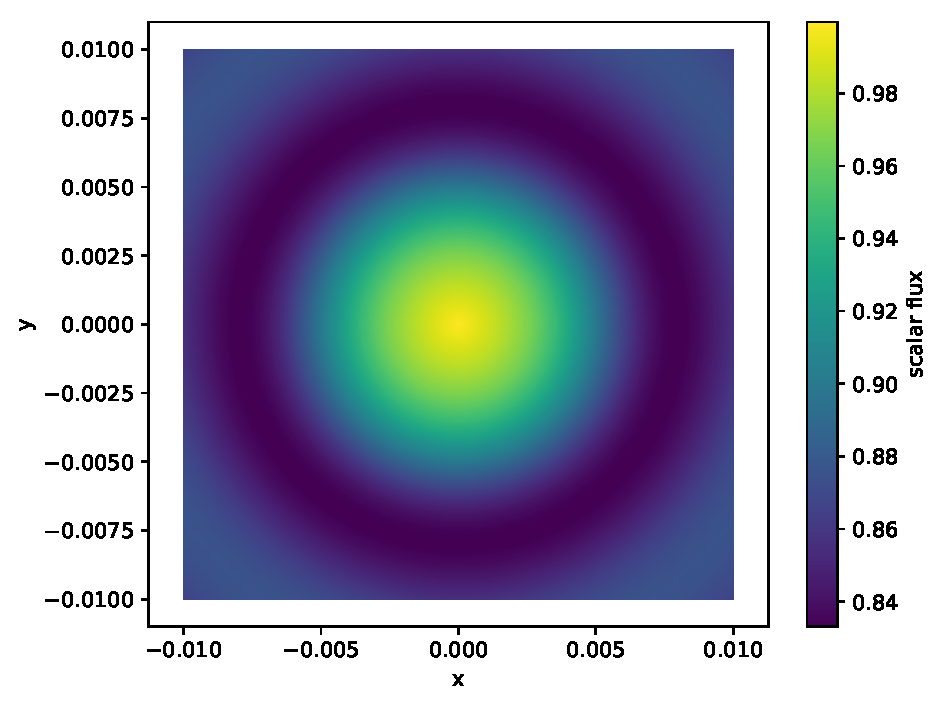
\includegraphics[width=0.47\textwidth]{figs/manufactured_ifba_solution_0}
\par\end{centering}
\label{fig:manufactured-radial-solution-1}}\hfill{}\subfloat[Thermal energy group]{\begin{centering}
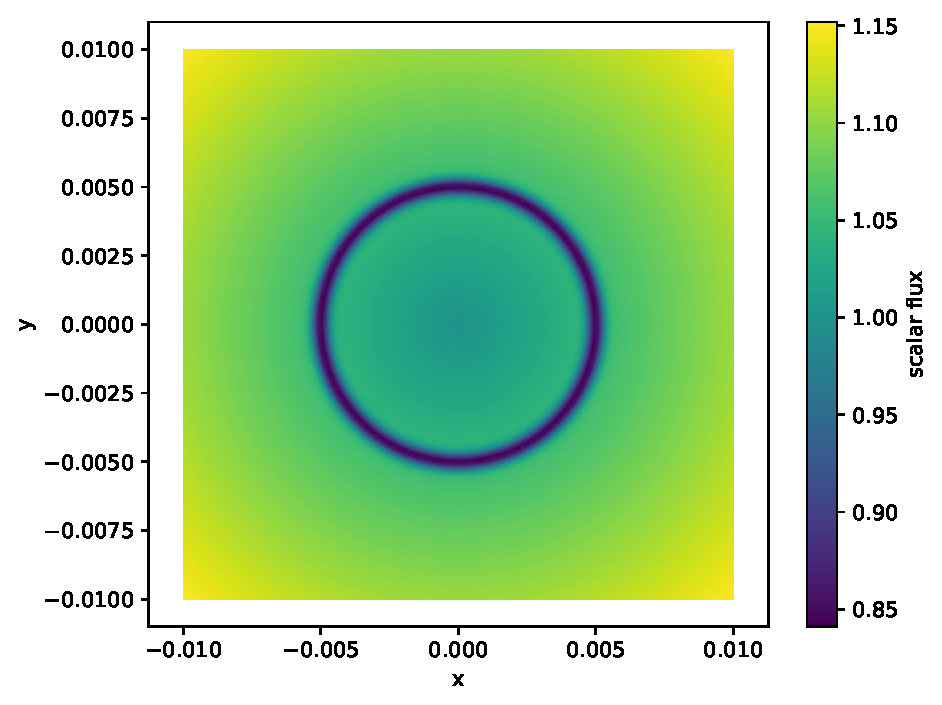
\includegraphics[width=0.47\textwidth]{figs/manufactured_ifba_solution_1}
\par\end{centering}
\label{fig:manufactured-radial-solution-2}}
\par\end{centering}
\caption{Solution to 2D manufactured radial problem}

\label{fig:manufactured-radial-solution}
\end{figure}

The second problem tests the ability of the code to reproduce a monoenergetic
sinusoidal function given continuous cross sections. The domain is
$\bm{x}\in\left[-2,2\right]$ and the solution is of the form
\begin{align}
\Phi_{\ell}^{m}\left(\bm{x}\right) & =f_{\ell}^{m}\left(1+\frac{1}{5}\cos\left(\pi x\right)\cos\left(\frac{\pi}{5}y\right)\cos\left(\frac{2\pi}{5}z\right)\right),\label{eq:manufactured-sinusoidal-sol}
\end{align}
with the $f_{\ell}^{m}$ constants from Table \ref{tab:manufactured-sinusoidal-sol}.
This results in a single period for the sinusoidal function in the
$x$ dimension and less than half a period in the $y$ and $z$ dimensions
(Fig. \ref{fig:manufactured-sinusoidal-solution}). The cross sections
are 
\begin{equation}
\Sigma\left(\bm{x}\right)=\Sigma_{0}\left(1+\frac{1}{2}\cos\left(\frac{\pi}{5}x\right)\cos\left(\frac{6\pi}{5}y\right)\cos\left(\frac{2\pi}{5}z\right)\right),\label{eq:manufactured-sinusoidal-xs}
\end{equation}
where $\Sigma_{0}$ is represents the base value of each cross section
from Table \ref{tab:manufactured-sinusoidal-xs} and $\Sigma$ represents
the spatially-dependent value of this cross section (e.g. to calculate
$\Sigma_{s;1}\left(\bm{x}\right)$, $\Sigma_{0}$ is set to the corresponding
value of 0.07 from the table). 

\begin{table}[!tb]
\caption{Manufactured solution and cross section data for sinusoidal problem}

\centering{} \captionsetup{width=.3\linewidth}\subfloat[{Solution coefficients {[}see Eq. (\ref{eq:manufactured-sinusoidal-sol}){]}}]{
\centering{}%
\begin{tabular}{|c|c|c|c|}
\hline 
$f_{0}^{0}$ & $f_{1}^{-1}$ & $f_{1}^{0}$ & $f_{1}^{1}$\tabularnewline
\hline 
\hline 
1.0 & 0.01 & 0.1 & -0.05\tabularnewline
\hline 
\end{tabular}\label{tab:manufactured-sinusoidal-sol}}\hspace{4em}\subfloat[{Cross sections {[}see Eq. (\ref{eq:manufactured-sinusoidal-xs}){]}}]{
\centering{}%
\begin{tabular}{|c|c|c|c|}
\hline 
$\Sigma_{t}$ & $\Sigma_{s;0}$ & $\Sigma_{s;1}$ & $\nu\Sigma_{f}$\tabularnewline
\hline 
\hline 
1.0 & 0.5 & 0.07 & 0.0\tabularnewline
\hline 
\end{tabular}\label{tab:manufactured-sinusoidal-xs}}
\end{table}

\begin{figure}[!tb]
\begin{centering}
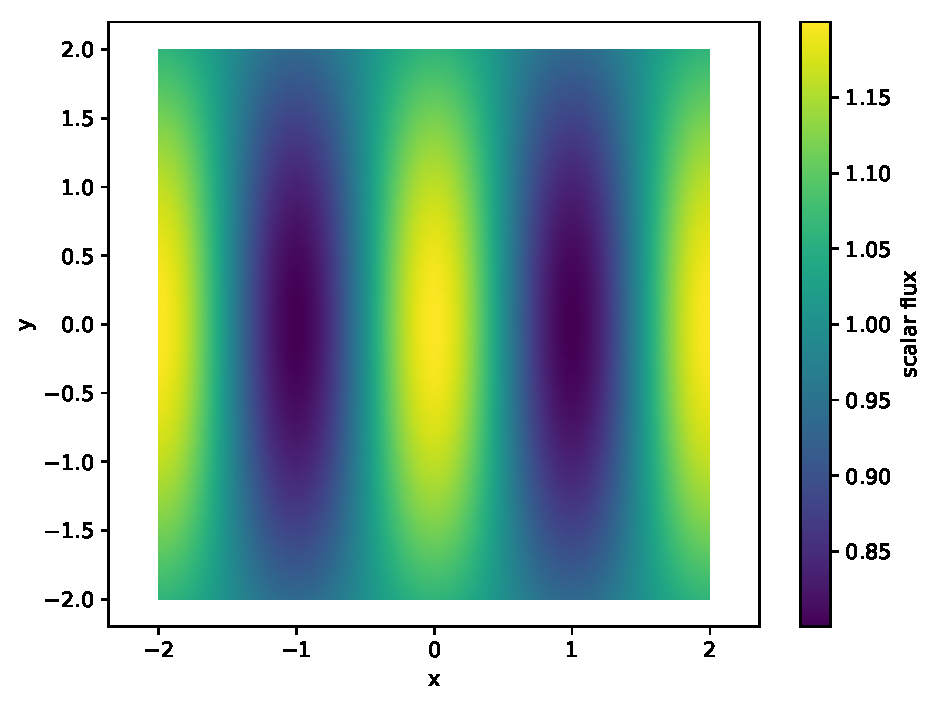
\includegraphics[width=0.47\textwidth]{figs/manufactured_sinudoidal_solution}
\par\end{centering}
\caption{Solution to 2D manufactured sinusoidal problem}
\label{fig:manufactured-sinusoidal-solution}
\end{figure}

Both problems include linearly anisotropic scattering. As described
in Sec. \ref{sec:method-of-manufactured}, the manufactured internal
source requires that the solution be performed with an additional
scattering moment above the scattering order, which raises the total
number of spherical harmonic moments in the solution from three to
six in 2D and from four to nine in 3D. These additional moments are
expected to have a numerical solution near zero for the converged
transport solution. The following results use the scalar flux for
the error calculation, as shown in Eq. (\ref{eq:l1-error-manufactured}).
For all cases, the first spherical harmonics moments of the equation
have similar errors to the scalar flux and the additional moments
have values near zero.

\subsection{Results for manufactured problems\label{subsec:manufactured-results}}

These results include optimization for the radii of the basis and
weight functions, optimization for the \gls{supg} parameters, convergence
results and summary of parameters for use in more realistic problems.
The radial and sinusoidal results are presented together for comparison
of the effect of continuous and discontinuous cross sections on the
weak and strong discretization methods.

\subsubsection{Optimization for the number of neighbors}

To find an accurate value for the number of neighbors in the radius
calculation (Alg. \ref{alg:radius-calculation}) for the weak form,
the value is varied between 8 to 20 neighbors in 2D and 12 to 26 neighbors
in 3D. For the \gls{mlpg} solution, the \gls{supg} stabilization
parameter is fixed at $\tau=r_{j}$, or $c=1$ in Eq. (\ref{eq:tau-radius}),
and the number of points is fixed at 4096 for the 2D problems and
for the 3D radial problem and 32768 for the 3D sinusoidal problem.
The full cross section weighting technique is used for all problems. 

\begin{figure}[!b]
\begin{centering}
\subfloat[Radial problem, 2D, 4096 points]{\begin{centering}
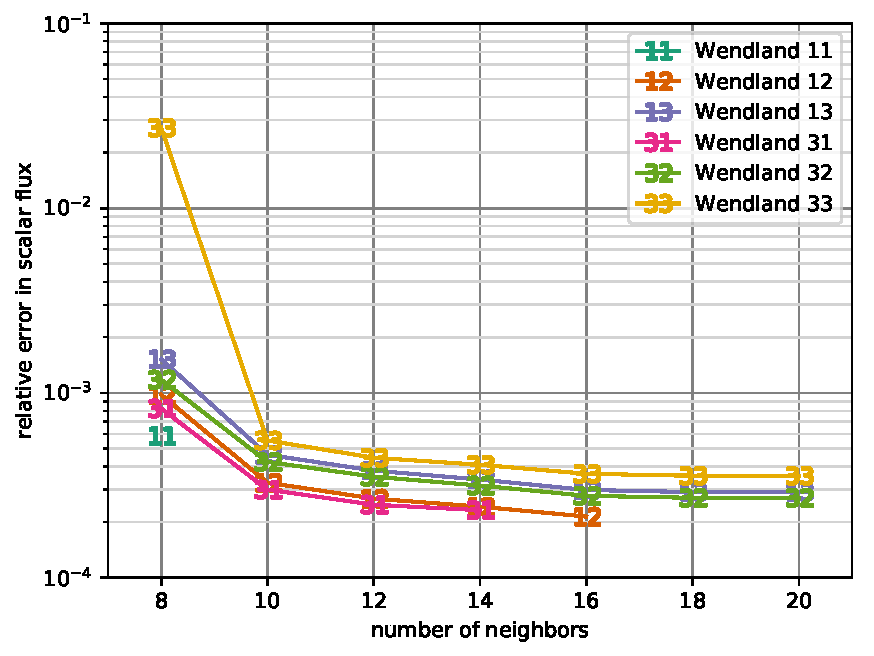
\includegraphics[width=0.47\textwidth]{figs/manufactured_ifba_neighbors_2d_64}
\par\end{centering}
\label{fig:manufactured-radial-neighbors-2d}}\hfill{}\subfloat[Sinusoidal problem, 2D, 4096 points]{\begin{centering}
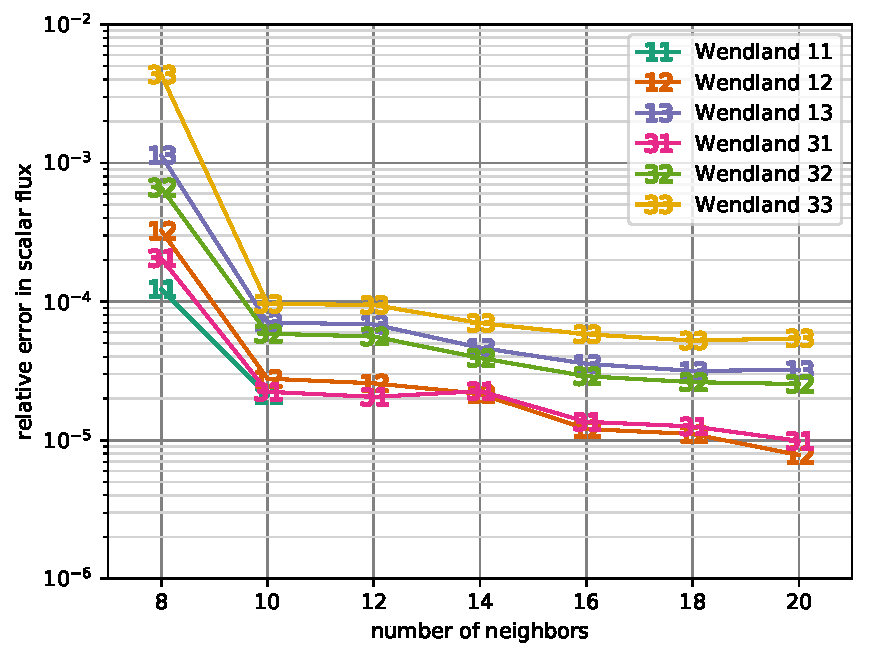
\includegraphics[width=0.47\textwidth]{figs/manufactured_sinusoidal_neighbors_2d_64}
\par\end{centering}
\label{fig:manufactured-sinusoidal-neighbors-2d}}
\par\end{centering}
\begin{centering}
\subfloat[Radial problem, 3D, 4096 points]{\begin{centering}
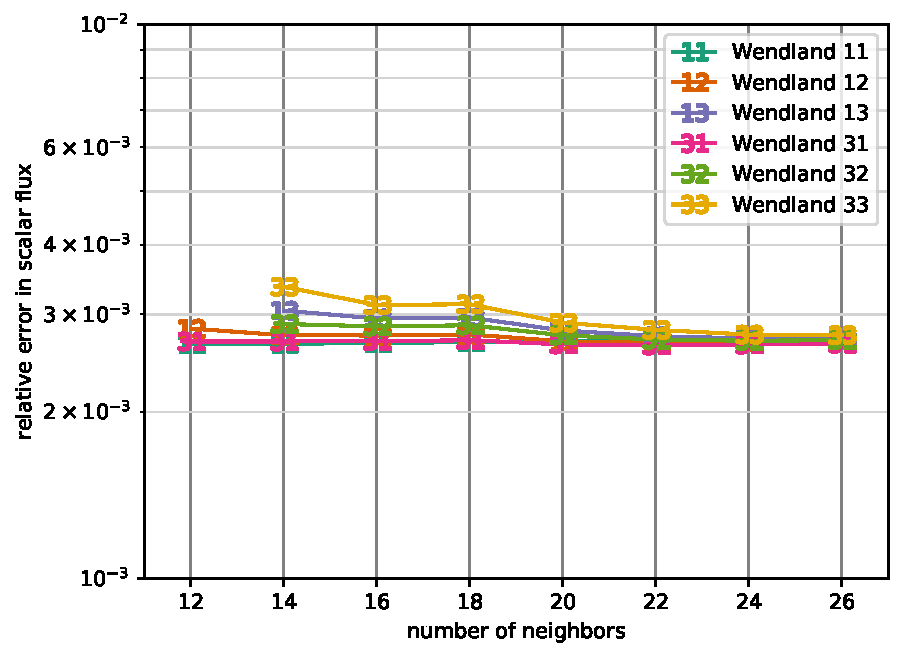
\includegraphics[width=0.47\textwidth]{figs/manufactured_ifba_neighbors_3d_16}
\par\end{centering}
\label{fig:manufactured-radial-neighbors-3d}}\hfill{}\subfloat[Sinusoidal problem, 3D, 32768 points]{\begin{centering}
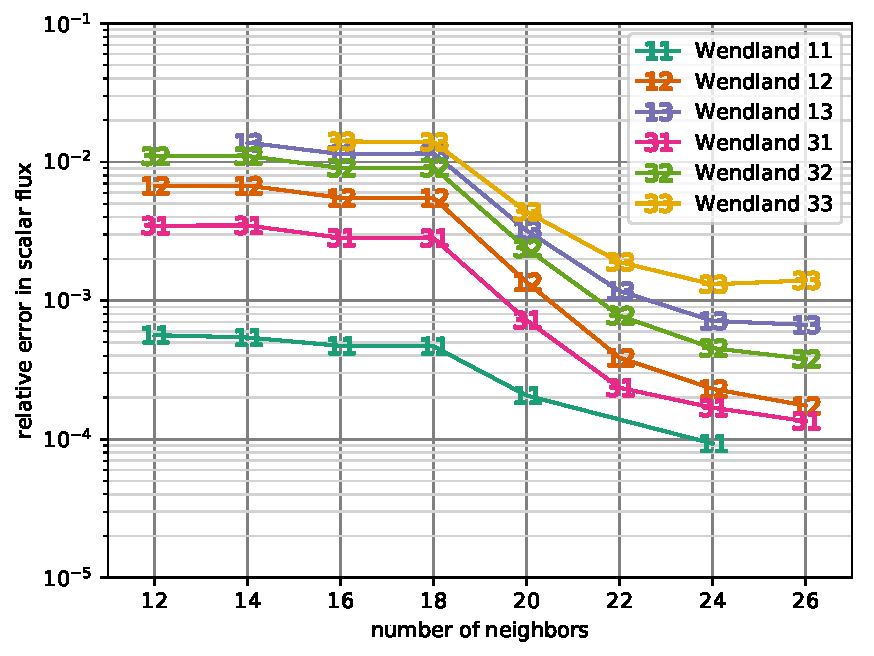
\includegraphics[width=0.47\textwidth]{figs/manufactured_sinusoidal_neighbors_3d_32}
\par\end{centering}
\label{fig:manufactured-sinusoidal-neighbors-3d}}
\par\end{centering}
\caption{Dependence of the error of the manufactured problems on number of
neighbors in the radius calculation, weak form}
\end{figure}

For the 2D radial problem (Fig. \ref{fig:manufactured-radial-neighbors-2d})
solution by the \gls{mlpg} equations, the Wendland 11 function shows
the best agreement with the manufactured solution at 8 neighbors,
with just about $10^{-4}$ relative error in the solution. For 10
to 14 neighbors, the Wendland 31 function is the optimal choice at
around $2\times10^{-5}$ relative error. For the 2D sinusoidal problem
(Fig. \ref{fig:manufactured-sinusoidal-neighbors-2d}), the Wendland
11 function shows the best agreement for 8 to 10 neighbors and Wendland
31 function is again better for more neighbors. For the radial and
sinusoidal problems, the Wendland 11 function does not converge for
more than 10 or 12 neighbors, respectively. For the 3D radial problem
(Fig. \ref{fig:manufactured-radial-neighbors-3d}), the Wendland11
and Wendland 31 functions perform similarly well, but the results
are relatively agnostic to the basis function and have around $3\times10^{-3}$
error for most Wendland function and radius choices. Finally, for
the 3D sinusoidal problem the results between basis and weight functions
differ more significantly, likely due to the higher number of points.
The Wendland 11 function performs best by almost an order of magnitude,
at around $5\times10^{-4}$ relative error for 12 to 18 neighbors
and then decreasing to less than $10^{-4}$ for 24 neighbors.

\begin{figure}[!b]
\begin{centering}
\subfloat[Radial problem, 2D, 4096 points]{\begin{centering}
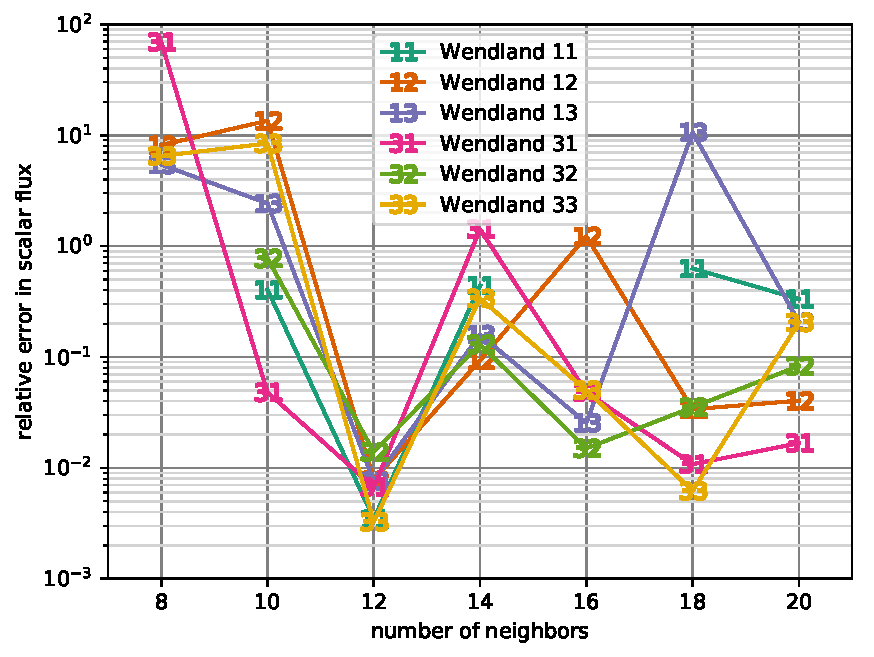
\includegraphics[width=0.47\textwidth]{figs/manufactured_ifba_strong_neighbors_2d_64}
\par\end{centering}
\label{fig:manufactured-radial-neighbors-strong-2d}}\hfill{}\subfloat[Sinusoidal problem, 2D, 4096 points]{\begin{centering}
\includegraphics[width=0.47\textwidth]{figs/manufactured_sinusoidal_strong_neighbors_2d_64}
\par\end{centering}
\label{fig:manufactured-sinusoidal-neighbors-strong-2d}}
\par\end{centering}
\begin{centering}
\subfloat[Radial problem, 3D, 4096 points]{\begin{centering}
\includegraphics[width=0.47\textwidth]{figs/manufactured_ifba_strong_neighbors_3d_16}
\par\end{centering}
\label{fig:manufactured-radial-neighbors-strong-3d}}\hfill{}\subfloat[Sinusoidal problem, 3D, 32768 points]{\begin{centering}
\includegraphics[width=0.47\textwidth]{figs/manufactured_sinusoidal_strong_neighbors_3d_32}
\par\end{centering}
\label{fig:manufactured-sinusoidal-neighbors-strong-3d}}
\par\end{centering}
\caption{Dependence of the error of the manufactured problems on number of
neighbors in the radius calculation, strong form}
\end{figure}

Compared to the weak discretization, the strong discretization depends
much more on an optimal choice for the number of neighbors to get
an accurate solution for problems with large gradients and material
discontinuities. The point weighting is used for the strong-form neighbor
calculations. In 2D, the sinusoidal problem (Fig. \ref{fig:manufactured-sinusoidal-neighbors-strong-2d})
has a large range of acceptable neighbor parameters from 10 to 20
for which the relative error of the solution is below $10^{-3}$.
In comparison, for the radial problem (Fig. \ref{fig:manufactured-radial-neighbors-strong-2d})
the error of the solution depends strongly on the number of neighbors.
Only for 12 neighbors do all the basis functions produce results below
$10^{-2}$ relative error for more than one basis function choice.
By changing the number of neighbors from this value by only two in
the radius calculation, the error increases for some basis functions
to around 10 times larger than the solution itself. 

This chaotic behavior of the solution with respect to the shape parameter
is shown more clearly in the 3D results. The sinusoidal problem behaves
normally (Fig. \ref{fig:manufactured-sinusoidal-neighbors-strong-3d})
and achieves error of below $10^{-3}$ for any number of neighbors
with the Wendland 11 function. The other functions converge to similar
values by 20 to 24 neighbors. For the radial problem (Fig. \ref{fig:manufactured-radial-neighbors-strong-3d}),
the scattering source did not converge any number of neighbors less
than 18. For the solutions that did converge, only one is below $10^{-1}$
in relative error, which may be due to cancellation of error. This
chaotic nature of the solution is likely not instability in the linear
solve of the $\mathcal{L}^{-1}$ operator, which is performed by a
direct solve for the strong problems (see Sec. \ref{subsec:transport-sweep-operator}).
Instead, this is an incorrect result given by the $\mathcal{L}^{-1}$
operator for a majority of parameters. This may be due to the lack
of integration to account for the materials accurately or due to instabilities
that propagate through the problem caused by localized gradients.
In either case, the results indicate poor performance for the strong
form discretization as presented in Sec. \ref{subsec:strong-discretization}
for problems with discontinuities and localized gradients. The strong
method may still be applicable to problems with continuous cross sections
and smooth solutions, such as the sinusoidal problem presented here.

\subsubsection{Optimization for the stabilization parameter}

The relative error with respect to the \gls{supg} parameter {[}Eq.
(\ref{eq:tau-radius}){]} for the weak form is shown for the radial
and sinusoidal problems in Figs. \ref{fig:manufactured-radial-tau-2d}
and \ref{fig:manufactured-sinusoidal-tau-2d}, respectively. These
results use the Wendland 31 function with 12 neighbors and full cross
section weighting. In both cases, the result of the calculation is
largely unchanged by the value of $\tau$ from about $c=1.0$ to $c=2.0$.
However, the iterative $\mathcal{L}^{-1}$ solve did not converge
for many of the $c=0.0$ to $c=0.75$ problems due to ill-conditioning.
For a low number of points, the weak form without \gls{supg} stabilization
($c=0.0$) produces acceptable results. As the number of points increases,
the results without stabilization do not converge. When a direct solver
is applied to the problems without stabilization, oscillations appear
throughout the problems, again signifying ill-conditioning issues
inherent to the numerical solution of advection problems without stabilization. 

\begin{figure}[!tb]
\begin{centering}
\subfloat[Radial problem]{\begin{centering}
\includegraphics[width=0.45\columnwidth]{figs/manufactured_ifba_tau_2d}
\par\end{centering}
\label{fig:manufactured-radial-tau-2d}}\hfill{}\subfloat[Sinusoidal problem]{\begin{centering}
\includegraphics[width=0.47\textwidth]{figs/manufactured_sinusoidal_tau_2d}
\par\end{centering}
\label{fig:manufactured-sinusoidal-tau-2d}}
\par\end{centering}
\caption{Dependence of the error of the 2D manufactured problems on the SUPG
constant $\tau$}
\end{figure}

These results suggest that while the \gls{supg} stabilization is
important in achieving good conditioning and low errors, the selection
of the parameter governing how much stabilization is added is not
of paramount importance. These same results hold for other choices
of Wendland function and number of neighbors.

\subsubsection{Convergence results}

Using functions and neighbor choices based on the parametric studies
from this section, convergence results are calculated for each problem
and discretization in two and three dimensions . The weak discretization
uses the Wendland 31 function with an \gls{supg} parameter of $c=1.0$.
The strong discretization uses the Wendland 33 function for the 2D
results and the Wendland 31 function for the 3D results. For the 2D
problems, 12 neighbors are used for each of the strong and weak discretizations.
For 3D problems, the weak form uses 14 neighbors for the radial problem
and 24 for the sinusoidal, while the strong form uses 20 neighbors
for the radial problem and 24 for the sinusoidal. The strong-form
results are limited to a relatively low number of points due to the
high computational cost of the direct solve used in the $\mathcal{L}^{-1}$
operator. 

In two dimensions, both the strong and weak discretizations converge
with approximately second-order accuracy for the radial problem (Fig.
\ref{fig:manufactured-radial-convergence-2d}). The weak form converges
for other functions and neighbors, while the strong form for other
functions and neighbors often diverges. The problems with basis weighting
of the cross sections converge more slowly than those with the full
and point weighting for the weak and strong forms, respectively. The
strong form with either cross section weighting performs over an order
of magnitude worse than the weak form with full cross section weighting.
The results for the sinusoidal problem in 2D (Fig. \ref{fig:manufactured-sinusoidal-convergence-2d})
also indicate second-order convergence. As before, the strong discretization
for the sinusoidal problem with either weighting has more than an
order of magnitude higher error than the weak form with full cross
section weighting. 

\begin{figure}[!tb]
\begin{centering}
\subfloat[Radial problem, 2D]{\begin{centering}
\includegraphics[width=0.47\textwidth]{figs/manufactured_ifba_convergence_2d}
\par\end{centering}
\label{fig:manufactured-radial-convergence-2d}}\hfill{}\subfloat[Sinusoidal problem, 2D]{\begin{centering}
\includegraphics[width=0.47\textwidth]{figs/manufactured_sinusoidal_convergence_2d}
\par\end{centering}
\label{fig:manufactured-sinusoidal-convergence-2d}}
\par\end{centering}
\begin{centering}
\subfloat[Radial problem, 3D]{\begin{centering}
\includegraphics[width=0.47\textwidth]{figs/manufactured_ifba_convergence_3d}
\par\end{centering}
\label{fig:manufactured-radial-convergence-3d}}\hfill{}\subfloat[Sinusoidal problem, 3D]{\begin{centering}
\includegraphics[width=0.47\textwidth]{figs/manufactured_sinusoidal_convergence_3d}
\par\end{centering}
\label{fig:manufactured-sinusoidal-convergence-3d}}
\par\end{centering}
\caption{Convergence of the manufactured problems for the strong and weak discretizations}
\end{figure}

For the 3D results, the weak form uses the full cross section weighting
while the strong form uses the point cross section weighting. The
results for the radial problem in 3D (Fig. \ref{fig:manufactured-radial-convergence-3d})
do not show convergence to the manufactured solution. The weak-form
solution converges to $10^{-3}$ relative error at 32768 points. For
the sinusoidal problem in 3D (Fig. \ref{fig:manufactured-sinusoidal-convergence-3d}),
the strong-form solution converges to around $3\times10^{-3}$ relative
error at 4096 points. The weak form converges more quickly to $7\times10^{-4}$
error at 4096 points and less than $2\times10^{-4}$ error at 32768
points. 

\subsubsection{Parameters for realistic problems\label{subsec:parameters-for-realistic}}

The manufactured solution parameter studies inform the choice of parameters
for the problems in Chapters \ref{sec:steady-results} and \ref{sec:eigenvalue-results}.
For the \gls{mlpg} equations, the Wendland 11 function is used as
the weighting function for the \gls{mls} basis and weight functions
for many of the problems, as it performs well even at a low number
of neighbors. The number of neighbors is chosen as 8 for the 1D and
2D problems in Secs. \ref{subsec:shielding-1d} and \ref{subsec:vera}
and 12 to 14 for the 3D problems in Secs. \ref{subsec:kobayashi}
and \ref{subsec:ellipsoid}. The \gls{supg} multiplication factor
$c$ {[}Eq. (\ref{eq:tau-radius}){]} is set at 1.0 for most problems,
or the lowest value for which both the manufactured problems are stable
for a high number of points. For some difficult problems, a multiplication
factor of $c=1.5$ helps the $\mathcal{L}^{-1}$ iterative solution
converge more quickly. 

\cleardoublepage{}

\sectionspacing

\section{Results for steady-state problems\label{sec:steady-results}}

The steady-state problems included in this section include:
\begin{itemize}
\item A one-dimensional, homogeneous, purely-absorbing slab (Sec. \ref{subsec:homogeneous-1d});
\item A one-dimensional, heterogeneous slab (Sec. \ref{subsec:shielding-1d});
and
\item A three-dimensional Kobayashi problem with a void region (Sec. \ref{subsec:kobayashi}).
\end{itemize}
\begin{comment}
In comparison to the eigenvalue results in Chapter \ref{sec:eigenvalue-results},
which only provide the spatial variation but not the overall magnitude
for the eigenvector, the steady-state results for the moments of the
angular flux provide both the spatial variation and the magnitude.
\end{comment}
{} The homogeneous slab is compared against an analytic solution . The
heterogeneous slab is compared against a \gls{dfem} solution and
a Monte Carlo solution. The three-dimensional Kobayashi problem is
compared to analytic results for a purely-absorbing case and Monte
Carlo results for a partially-scattering case. 

The boundaries for the problems in this  chapter and for the eigenvalue
results in Chapter \ref{sec:eigenvalue-results} are exclusively Cartesian
planes. This is a simplification that reduces the complexity of reflection
and integration. The 2D and 3D \gls{ldfe} quadratures have quadrant
and octant symmetry, respectively. For the reflection angle from Eq.
(\ref{eq:reflection-angle}), Cartesian boundaries guarantee that
for any $\bm{\Omega}_{n}$, the reflection direction $\bm{\Omega}_{n_{r}}$
is also a member of the quadrature. The Cartesian boundaries also
allow simple integration of the domain and boundaries using a Cartesian
mesh. In addition, surfaces with a constant normal direction allow
for direction-independent surface integration for the basis and weight
functions. For arbitrary boundary surfaces, a more specialized integration
mesh and interpolation between angular directions would be required.

The general parameters for the slab and void problems are shown in
Table \ref{tab:general-parameters-steady}. As discussed in Chapter
\ref{sec:method-of-manufactured}, to maintain a large enough radius
for the basis and weight functions the number of neighbors for the
radius calculation should be larger for a higher-dimensional problem. 

\begin{table}[!tb]
\caption{Solution parameters for steady-state problems}

\centering{}%
\begin{tabular}{|c|c|c|c|c|}
\hline 
Parameter & Reference & Homogeneous & Heterogeneous & Kobayashi\tabularnewline
\hline 
\hline 
Num. neighbors for radius calculation & \multirow{2}{*}{Alg. \ref{alg:radius-calculation}} & \multicolumn{2}{c|}{8} & \multicolumn{1}{c|}{12\textendash 14}\tabularnewline
\cline{1-1} \cline{3-5} 
Multiplication factor for radius &  & \multicolumn{3}{c|}{1.0}\tabularnewline
\hline 
\gls{supg} multiplication factor $c$ & Eq. (\ref{eq:tau-radius}) & \multicolumn{3}{c|}{1.0}\tabularnewline
\hline 
$\mathcal{L}^{-1}$ convergence tolerance & Sec. \ref{subsec:transport-sweep-operator} & \multicolumn{2}{c|}{$10^{-12}$} & \multicolumn{1}{c|}{$10^{-10}$}\tabularnewline
\hline 
Solution convergence tolerance & Sec. \ref{subsec:outer-iterations} & - & $10^{-10}$ & \multicolumn{1}{c|}{$10^{-8}$}\tabularnewline
\hline 
Number of angular directions & Sec. \ref{subsec:energy-angular-physical} & 8192 & 256 & 512\tabularnewline
\cline{1-4} 
Wendland \gls{rbf} used to create \gls{mls} & Sec. \ref{subsec:meshless-functions} & 31 & \multicolumn{2}{c|}{11}\tabularnewline
\hline 
\end{tabular}\label{tab:general-parameters-steady}
\end{table}


\subsection{One-dimensional, homogeneous, purely-absorbing slab\label{subsec:homogeneous-1d}}

This slab-geometry problem is designed to test the ability of the
\gls{mlpg} discretization to calculate solutions in optically thick
and optically thin problems. The problem consists of a homogeneous,
one-group, purely-absorbing slab with a length of $L=1.0$, an isotropic
source of $\psi_{0}$ on the left side of the problem and no internal
source. The transport equation for this problem with the appropriate
boundary conditions can be written as\begin{subequations}
\begin{gather}
\mu\frac{\partial}{\partial x}\psi\left(x,\mu\right)+\Sigma_{t}\psi\left(x,\mu\right)=0,\qquad0\leq x\leq L,\quad-1\leq\mu\leq1,\\
\psi\left(x,\mu\right)\bigg|_{x=0}=\psi_{0},\qquad\mu>0,\\
\psi\left(x,\mu\right)\bigg|_{x=L}=0,\qquad\mu<0,
\end{gather}
\end{subequations}where $\mu$ is the angle cosine. The solution
to this problem is
\begin{equation}
\psi_{\text{exact}}\left(x,\mu\right)=\begin{cases}
\psi_{0}\exp\left(-\dfrac{\Sigma_{t}x}{\mu}\right), & \mu>0,\\
0, & \mu<0,
\end{cases}
\end{equation}
from which the scalar flux at any point in the problem can be calculated
by integrating over the angular cosine,
\begin{align}
\phi_{\text{exact}}\left(x\right) & =\int_{-1}^{1}\psi\left(x,\mu\right)d\mu\nonumber \\
 & =\int_{0}^{1}\psi_{0}\exp\left(-\frac{\Sigma_{t}x}{\mu}\right)d\mu.\label{eq:slab-scalar-flux}
\end{align}
This solution provides results to compare against for the numerical
simulations. 

The angular distribution of neutrons that reach the right edge of
the slab at $x=L$ is forward peaked for an optically thick problem
($\Sigma_{t}\gg1$), whereas for an optically thin problem ($\Sigma_{t}\ll1$),
the angular distribution of neutrons is relatively flat except near
$\mu\ll1$, for which the probability of a neutron reaching the far
side of the slab is very low. These distributions are shown in Fig.
\ref{fig:slab-angular distribution} for various total cross section
values. The angular integration of the $\Sigma_{t}=1.0$ case is straightforward
and does not require a large number of ordinates due to the approximately
linear shape of the function. The cases of $\Sigma_{t}=0.01$ and
$\Sigma_{t}=100$, however, have large gradients that require many
ordinates to accurately integrate. Because of this, 8192 angular ordinates
are used for this problem, as shown in Table \ref{tab:general-parameters-steady},
to limit the effect of the angular discretization on the accuracy
of the \gls{mlpg} solution. 

\begin{figure}[!tb]
\begin{centering}
\includegraphics[width=0.47\textwidth]{figs/slab_angular_distribution}
\par\end{centering}
\caption{Normalized angular distribution of neutrons exiting purely absorbing
slab for various cross sections}
\label{fig:slab-angular distribution}
\end{figure}

The problem is tested for the cross section cases of $\Sigma_{t}=0.01,\ 0.1,\ 1.0,\ 10.0,\ 100.0$
and between 8 and 512 points. Because the problem is purely absorbing,
the solution converges after a single outer iteration. The solution
for the scalar flux at the right boundary of the problem, $\phi\left(L\right)$,
is compared to the analytic solution from Eq. (\ref{eq:slab-scalar-flux})
using the relative error
\begin{equation}
\epsilon=\frac{\left|\phi_{\text{exact}}\left(L\right)-\phi\left(L\right)\right|}{\phi_{\text{exact}}\left(L\right)}.
\end{equation}
The values for the exact scalar flux at the right edge of the problem
range from $3.64782\times10^{-46}$ for $\Sigma_{t}=100$ to 0.999037
for $\Sigma_{t}=0.01$. 

Figure \ref{fig:slab-error} includes the error for \gls{mlpg}, strong-form
collocation and \gls{dfem} simulations. All three use the same angular
discretization. The relative errors for the \gls{mlpg} method are
below $10^{-4}$ by 64 points for all cross section cases except $\Sigma_{t}=100$,
which has a flux value at the boundary that is 46 orders of magnitude
lower than the initial boundary source and requires 512 points to
reach a relative error of $1.7\times10^{-4}$. Relative errors are
less than $10^{-8}$ by 512 points for cases with $\Sigma_{t}\leq1$.
The convergence rate of the \gls{mlpg} solution appears to be around
third-order. The solution converges much faster than this for a low
number of points. For the optically thin cases, the conditioning of
the problem appears to become worse for 256 to 512 points, causing
the error to increase slightly. 

\begin{figure}[!tb]
\begin{centering}
\subfloat[MLPG]{\begin{centering}
\includegraphics[width=0.47\textwidth]{figs/slab_error}
\par\end{centering}
}\hfill{}\subfloat[Strong-form collocation]{\begin{centering}
\includegraphics[width=0.47\textwidth]{figs/slab_error_strong}
\par\end{centering}
}
\par\end{centering}
\begin{centering}
\subfloat[Linear DFEM, for comparison]{\begin{centering}
\includegraphics[width=0.47\textwidth]{figs/slab_error_dfem}
\par\end{centering}
}
\par\end{centering}
\caption{Relative error in scalar flux for neutrons exiting purely absorbing
slab for various cross sections}

\label{fig:slab-error}
\end{figure}

The relative error for the collocation method is around two to three
orders of magnitude larger than the error for the \gls{mlpg} method
for a similar number of points. For a large number of points, the
collocation method seems to not converge past $10^{-6}$ relative
error, possibly due to numerical conditioning issues. For the optically-thick
$\Sigma_{t}=100$ case, the collocation method requires almost ten
times as many points as the \gls{mlpg} method to converge to $10^{-2}$
error. There is not a clear enough pattern in the results to calculate
a convergence rate of the solution with any confidence. 

The \gls{dfem} solution shows exactly second-order convergence for
the $\Sigma_{t}\leq10$ cases. For $\Sigma_{t}=100$, the numerical
solution is zero regardless of the number of points, which may be
due to the mass matrix lumping technique employed to prevent negative
solutions (See Ref. \cite{adams-discontinuous-2001} for details).
For a similar number of spatial unknown values (two per element for
the \gls{dfem} solution), the \gls{mlpg} solution has between two
and four orders of magnitude lower error than the \gls{dfem} solution.
The smallest two numbers of elements shown for the \gls{dfem} solution
have the same number of unknowns as the largest two for the \gls{mlpg}
solution. For this problem, the errors are similar for 64 spatial
points in the \gls{mlpg} method and 2048 elements in the linear \gls{dfem}
method. 

\subsection{One-dimensional, heterogeneous slab reactor\label{subsec:shielding-1d}}

The second problem is a one-dimensional, two-group, steady-state slab,
with geometry shown in Fig. \ref{fig:shielding1d-geometry} and and
cross sections listed in Table \ref{tab:shielding1d-xs}. The boundary
conditions on the left and right are reflective and vacuum, respectively.
The source region represents a multiplicative medium whose fast neutrons
are moderated to thermal energies in the moderator region. The thermalized
neutrons are then captured by the absorber. The solution for the problem
in Fig. \ref{fig:shielding1d-solution} is consistent with the expected
birth of fast neutrons in the source region, the transfer to the thermal
group in the moderator region and the preferential absorption of thermal
neutrons in the absorber region. 

\begin{table}[!b]
\caption{Heterogeneous slab cross sections}

\centering{}%
\begin{tabular}{|c|c|c|c|c|c|c|c|c|c|}
\hline 
Mat. & $g$ & $\Sigma_{t;g}$ & $\Sigma_{s;0,g\to1}$ & $\Sigma_{s;0,g\to2}$ & $\Sigma_{s;1,g\to1}$ & $\Sigma_{s;1,g\to2}$ & $\chi\nu\Sigma_{f;g\to1}$ & $\chi\nu\Sigma_{f;g\to2}$ & $Q_{g}$\tabularnewline
\hline 
\hline 
\multirow{2}{*}{Sou.} & 1 & 1.0 & 0.9 & 0.05 & 0.1 & 0.0 & 0.0 & 0.0 & 1.0\tabularnewline
\cline{2-10} 
 & 2 & 2.0 & 0.05 & 0.8 & 0.0 & 0.0 & 1.0 & 0.0 & 0.0\tabularnewline
\hline 
\multirow{2}{*}{Mod.} & 1 & 0.5 & 0.05 & 0.45 & 0.0 & 0.1 & 0.0 & 0.0 & 0.0\tabularnewline
\cline{2-10} 
 & 2 & 1.0 & 0.0 & 1.0 & 0.0 & 0.01 & 0.0 & 0.0 & 0.0\tabularnewline
\hline 
\multirow{2}{*}{Abs.} & 1 & 0.5 & 0.0 & 0.0 & 0.0 & 0.0 & 0.0 & 0.0 & 0.0\tabularnewline
\cline{2-10} 
 & 2 & 10.0 & 0.0 & 0.0 & 0.0 & 0.0 & 0.0 & 0.0 & 0.0\tabularnewline
\hline 
\end{tabular}\label{tab:shielding1d-xs}
\end{table}

\begin{figure}[!b]
\begin{centering}
\includegraphics[width=0.5\textwidth]{figs/shielding1d_geometry}
\par\end{centering}
\caption{Heterogeneous slab geometry}
\label{fig:shielding1d-geometry}
\end{figure}

\begin{figure}[!tb]
\begin{minipage}[b][1\totalheight][t]{0.47\columnwidth}%
\includegraphics[width=1\textwidth]{figs/shielding1d_solution}

\caption{Heterogeneous slab solution, 5120 points}

\label{fig:shielding1d-solution}%
\end{minipage}\hfill{}%
\begin{minipage}[b][1\totalheight][t]{0.47\columnwidth}%
\begin{center}
\includegraphics[width=1\textwidth]{figs/shielding1d_convergence}
\par\end{center}
\caption{Heterogeneous slab convergence}

\label{fig:shielding1d-convergence}%
\end{minipage}
\end{figure}

The benchmark solution for the one-dimensional problem is generated
using a \gls{dfem} code with 500000 elements and linear basis and
weight functions within each element. The average solution $\bar{\phi}_{i,g}^{\text{bench}}$
over 1000 overlaid cells with index $i$ for each energy group $g$
is then calculated. After completion of the \gls{mlpg} solution,
the average scalar flux $\bar{\phi}_{i,g}$ across each of the same
regions is calculated by integration with a 64-point Gauss-Legendre
quadrature. Finally, the $L_{2}$ error of the meshless solution with
respect to the benchmark solution is calculated as 
\begin{equation}
\left(L_{2}\text{ error}\right)_{g}=\left(\frac{\sum_{i}\left(\bar{\phi}_{i,g}-\bar{\phi}_{i,g}^{\text{bench}}\right)^{2}}{\sum_{i}\left(\bar{\phi}_{i,g}^{\text{bench}}\right)^{2}}\right)^{1/2}.\label{eq:l2-error}
\end{equation}

With the solution parameters in Table \ref{tab:general-parameters-steady},
a convergence study for the number of points is performed for each
of the basis and full cross section weightings as described in Sec.
\ref{subsec:cross-section-discretization}. The points are placed
evenly throughout the problem. The convergence results in Fig. \ref{fig:shielding1d-convergence}
show second-order convergence with the point spacing for both types
of cross section weighting. Similarly to the \gls{mms} problems,
the full cross section weighting has lower error than the basis weighting,
in this case by more than and order of magnitude. The cellwise relative
error is around an order of magnitude larger than the $L_{2}$ error
near large gradients, for the fast group at the source/moderator boundary
and for the thermal group at the moderator/absorber boundary. 

For 5120 points and full cross section weighting, the $L_{2}$ error
is $8.71\times10^{-7}$ and $1.93\times10^{-6}$ for the fast and
thermal groups, respectively. For comparison, the $L_{2}$ errors
of a 5000-element \gls{dfem} solution, which has almost twice as
many degrees of freedom as the 5120-point meshless solution, are $1.45\times10^{-6}$
and $2.71\times10^{-6}$. However, the \gls{dfem} solution requires
about 12 seconds, compared to 32 or 50 for the \gls{mlpg} solution,
depending on whether a direct or iterative solver is used for the
$\mathcal{L}^{-1}$ operator. 

To quantify the expected error for the two and three dimensional problems
in the following section that use Monte Carlo benchmarks, the convergence
for this one-dimensional problem to the \gls{dfem} method is compared
to the convergence to a Monte Carlo solution. The results of the \gls{mlpg}
method converge more quickly to a similar deterministic solution for
a fixed angular quadrature rule than to a Monte Carlo solution. For
this one-dimensional problem, a Monte Carlo calculation using the
multigroup mode of OpenMC \cite{romano-openmc-2013} is performed
and tallies over the same 1000 cells as before with 100 generations
and $10^{7}$ particles per generation are compared to the \gls{dfem}
(500000 elements) and \gls{mlpg} results (10240 points). The $L_{2}$
error from the Monte Carlo solution is the same for both to the fifth
decimal place, at $4.9\times10^{-4}$ for the fast and $2.1\times10^{-4}$
for the thermal group. The standard deviation of the Monte Carlo flux
tally does not exceed $1.6\times10^{-4}$ for any tally cell or group
and is, on average, $3.2\times10^{-5}$ for the fast group and $6.2\times10^{-5}$
for the thermal group. This indicates that the difference between
the deterministic and Monte Carlo calculations is likely not random
noise, but instead angular error introduced by the discrete ordinates
approximation. For the two and three dimensional problems, good but
not complete convergence of the \gls{mlpg} method to the Monte Carlo
solution is similarly expected. 

\subsection{Three-dimensional Kobayashi problem with void region\label{subsec:kobayashi}}

The three-dimensional Kobayashi benchmark problems \cite{kobayashi-3d-2001}
are designed to test deterministic codes in the presence of void regions.
Problem 1 of the Kobayashi set, which is considered here, includes
a cubic source at the center, a surrounding void region and a shield
(Fig. \ref{fig:kobayashi-geometry} and Table \ref{tab:kobayashi-xs}).
The cross sections are either purely absorbing or partially scattering.
The boundary conditions for the planes at $x,y,z=0$ cm are reflective,
while the boundary conditions for the planes at $x,y,z=100$ cm are
vacuum. 

\begin{table}[!b]
\caption{Kobayashi cross sections}

\centering{}%
\begin{tabular}{|c|c|c|c|c|}
\hline 
Mat. & $\Sigma_{t}$ & $\Sigma_{s}$ (abs) & $\Sigma_{s}$ (sca) & $Q$\tabularnewline
\hline 
\hline 
Source & 0.1 & 0.0 & 0.05 & 1.0\tabularnewline
\hline 
Void & 0.0001 & 0.0 & 0.00005 & 0.0\tabularnewline
\hline 
Shield & 0.1 & 0.0 & 0.05 & 0.0\tabularnewline
\hline 
\end{tabular}\label{tab:kobayashi-xs}
\end{table}

\begin{figure}[!b]
\begin{centering}
\includegraphics[width=0.56\textwidth]{figs/kobayashi_p1_problem}
\par\end{centering}
\caption{Kobayashi geometry and evaluation points}
\label{fig:kobayashi-geometry}
\end{figure}

The centers for the Kobayashi problem are a simple Cartesian grid
of points. The number of neighbors for the radius calculation is increased
to between 12 and 14 for this 3D case to maintain the same general
radius for a evenly-spaced points (Table \ref{tab:general-parameters-steady}),
as discussed in Sec. \ref{subsec:parameters-for-realistic}. The scalar
flux is calculated at specific points in the problem (which contrasts
with the integral approach from Secs. \ref{subsec:shielding-1d} and
\ref{subsec:ellipsoid}) for comparison against the benchmark results
at these same points from Kobayashi and Sugimura \cite{kobayashi-3d-2001}.
The given benchmarks are analytic for the purely absorbing case and
are calculated by the Monte Carlo code GMVP for the scattering case.
The overall $L_{2}$ error is calculated according to Eq. (\ref{eq:l2-error})
with integrated values replaced by discrete values. 

\subsubsection{Convergence with spatial refinement\label{subsec:kobayashi-spatial}}

The convergence of these $L_{2}$ values for the absorbing and the
scattering cases is shown in Fig. \ref{fig:kobayashi-convergence}.
The dependence on only a few pointwise quantities makes the $L_{2}$
error more volatile than previous problems, which use global or integrated
quantities. The convergence plot shows several dips in the error at
certain point values with full weighting, with minima at $16^{3}$,
$22^{3}$ and $40^{3}$ points. These irregularities in the convergence
make determination of convergence rates difficult. An exponential
function fit over the last ten data points (from $32^{3}$ to $42^{3}$
points) predicts at least second-order convergence with point spacing
for all cases. 

\begin{figure}[!b]
\begin{centering}
\includegraphics[width=0.47\textwidth]{figs/kobayashi_convergence}
\par\end{centering}
\caption{Kobayashi convergence with spatial refinement, 512 directions}
\label{fig:kobayashi-convergence}
\end{figure}

For the case with the most points, the largest relative error of around
100 percent occurs at the evaluation point $\left(95\ ,95,\ 95\right)$,
which is at the furthest corner of the problem from the source and
has a benchmark value of $3.01032\times10^{-6}$ for the absorbing
problem and $1.12892\times10^{-5}$ for the scattering problem. This
is also the point with the lowest absolute error. The evaluation point
at $\left(5,\ 5,\ 5\right)$, inside the source, has benchmark values
of 5.95659 for the absorbing problem and 8.29260 for the scattering
problem. This is the point with the highest absolute error but the
lowest relative error, at around 0.15 percent and 0.10 percent for
the absorbing and scattering problems, respectively. 

\subsubsection{Convergence with angular refinement\label{subsec:kobayashi-angular}}

In problems with low scattering ratios, the flux is mostly uncollided.
For a problem in which a small detector (such as the point detectors
in this problem) is far from the neutron source, the detector may
only ``see'' the angular flux coming from a few directions. Rays
coming from other directions do not lead back to the source, and so
have values of zero. In Fig. \ref{fig:kobayashi-geometry-ray}, which
is the Kobayashi geometry simplified to flatland geometry, only one
of the rays that carries angular information to the point detector
has a nonzero value for the analytic case. Using the \gls{csg} described
in Appendix \ref{sec:constructive-solid-geometry} and a given quadrature,
the angular directions can be traced back to the original source region
to see how many of these directions contribute to the value of the
scalar flux in a purely absorbing medium. 

Figure \ref{fig:kobayashi-angular-points-ray} shows the total number
of directions with a nonzero value for a point detector at at various
positions. To have even 10 nonzero quadrature points at the detector
requires 8192 directions. As discussed in Chapter \ref{sec:integration-methods},
integration quadratures do not perform optimally in the presence of
discontinuities. Problems with ray effects have discontinuities in
the angular flux values, which degrades the performance of the discrete
ordinates solution. For the quadrature with 2048 points, even though
the point at $\left(95\ ,95,\ 95\right)$ has only a single quadrature
point that is nonzero for the purely absorbing case, the error should
still decrease compared to the lower-order quadratures as the angular
size of the source is known more accurately. 

\begin{figure}[!b]
\centering{}%
\begin{minipage}[b][1\totalheight][t]{0.47\columnwidth}%
\begin{center}
\includegraphics[width=1\textwidth]{figs/kobayashi_ray_geometry}
\par\end{center}
\caption{Ray effect diagram for the Kobayashi problem in a simplified flatland
geometry}
\label{fig:kobayashi-geometry-ray}%
\end{minipage}\hfill{}%
\begin{minipage}[b][1\totalheight][t]{0.47\columnwidth}%
\begin{center}
\includegraphics[width=1\textwidth]{figs/kobayashi_rays}
\par\end{center}
\caption{Number of nonzero angular quadrature points for a point detector in
the Kobayashi problem}
\label{fig:kobayashi-angular-points-ray}%
\end{minipage}
\end{figure}

The $L_{2}$ error applied for the spatial convergence study in Sec.
\ref{subsec:kobayashi-spatial} is biased toward the regions of highest
flux, which includes the points nearest to the source that are easiest
to converge. Using the the worst-case relative error,
\begin{equation}
L_{\infty}\text{ error}=\max_{i}\left(\left|\frac{\phi_{i}-\phi_{i}^{\text{bench}}}{\phi_{i}^{\text{bench}}}\right|\right),
\end{equation}
however, the solution does not converge for an increasing number of
points with a fixed angular quadrature rule. To show the effect of
the angular error on the problem, the same scattering and absorbing
problems are tested with between $10^{3}$ and $32^{3}$ points and
128 to 2048 directions (Fig. \ref{fig:kobayashi-angular}) 

\begin{figure}[!tb]
\begin{centering}
\subfloat[Absorbing]{\begin{centering}
\includegraphics[width=0.47\textwidth]{figs/kobayashi_angular_abs_linf_rel}
\par\end{centering}
}\hfill{}\subfloat[Partially scattering]{\begin{centering}
\includegraphics[width=0.47\textwidth]{figs/kobayashi_angular_sca_linf_rel}
\par\end{centering}
}
\par\end{centering}
\caption{Kobayashi convergence with angular refinement, full cross section
weighting}
\label{fig:kobayashi-angular}
\end{figure}

For 2048 directions the $L_{\infty}$ error decreases as more points
are added to the problem. For a 128 directions, however, the $L_{\infty}$
error is lowest for the cases with the fewest spatial points. This
is because the larger number of points causes accurate angular flux
values to reach the furthest detectors for only one or two quadrature
points, which the integration then incorrectly extrapolates to all
nearby angular directions. The basis and weight functions for the
smallest number of points (1000 points) have radii between 15 and
28 cm. This means the information from spatially integrating the basis
and weight functions over the source region (which is 10 cm by 10
cm for the reflected problem) is included in basis and weight functions
that have centers far from the source region. This blurring of the
source may add a few more nonzero quadrature points to the integration,
but also decreases the apparent source strength in the source region,
which is part of why the cases with few spatial points perform poorly
approximations of the closest points to the source region (see Sec.
\ref{subsec:kobayashi-spatial}). 

\cleardoublepage{}

\sectionspacing

\section{Results for eigenvalue problems\label{sec:eigenvalue-results}}

The eigenvalue problems considered in these results include:
\begin{itemize}
\item A two-dimensional pressurized water reactor (PWR) pincell in two geometries
(Secs. \ref{subsec:vera}\textendash \ref{subsec:vera-1e}) and
\item A three-dimensional reflected ellipsoid (Sec. \ref{subsec:ellipsoid}). 
\end{itemize}
Table \ref{tab:general-parameters-eigenvalue} summarizes the solution
parameters for each of the problems in this section, including the
number of neighbors for the radius calculation, the \gls{supg} multiplication
factor, and the solution convergence tolerance. Table \ref{tab:eigenvalue-errors}
shows the eigenvalue and eigenvector errors for the problems with
the most spatial points. Table \ref{tab:eigenvalue-benchmarks} and
\ref{tab:eigenvalue-benchmarks-continuous} show the multigroup and
continuous-energy Monte Carlo eigenvalue results, which are used as
benchmarks for the eigenvalue problems. As described for the steady-state
problems in Chapter \ref{sec:steady-results}, these problems use
Cartesian boundaries to simplify reflection at the boundaries and
integration of the basis and weight functions. 

\begin{table}[!b]
\caption{Solution parameters for $k$-eigenvalue problems}

\centering{}%
\begin{tabular}{|c|c|c|c|c|}
\hline 
Parameter & Reference & \gls{vera} 1B & \gls{vera} 1E & Ellipsoid\tabularnewline
\hline 
\hline 
Num. neighbors for radius calculation & \multirow{2}{*}{Alg. \ref{alg:radius-calculation}} & \multicolumn{2}{c|}{8} & \multicolumn{1}{c|}{12 / 14}\tabularnewline
\cline{1-1} \cline{3-5} 
Multiplication factor for radius &  & \multicolumn{3}{c|}{1.0}\tabularnewline
\hline 
\gls{supg} multiplication factor $c$ & Eq. (\ref{eq:tau-radius}) & 1.0 / 1.5 & 1.5 & 1.0\tabularnewline
\hline 
$\mathcal{L}^{-1}$ convergence tolerance & Sec. \ref{subsec:transport-sweep-operator} & \multicolumn{3}{c|}{$10^{-10}$}\tabularnewline
\hline 
Solution convergence tolerance & Sec. \ref{subsec:outer-iterations} & \multicolumn{3}{c|}{$10^{-8}$}\tabularnewline
\hline 
Number of angular directions & Sec. \ref{subsec:energy-angular-physical} & \multicolumn{2}{c|}{16\textendash 4096} & 512\tabularnewline
\hline 
Wendland \gls{rbf} used to create \gls{mls} & Sec. \ref{subsec:meshless-functions} & \multicolumn{2}{c|}{11} & 11 / 31\tabularnewline
\hline 
\end{tabular}\label{tab:general-parameters-eigenvalue}
\end{table}

\begin{table}[!p]
\caption{Continuous-energy Monte Carlo benchmark values for $k$-eigenvalue
problems}

\centering{}%
\begin{tabular}{|c|c|c|c|c|c|}
\cline{2-6} 
\multicolumn{1}{c|}{} & \multicolumn{2}{c|}{\gls{vera} 1B} & \multicolumn{2}{c|}{\gls{vera} 1E} & \multirow{2}{*}{Ellipsoid}\tabularnewline
\cline{1-5} 
\multicolumn{1}{|c|}{Value} & 600 K & 1200 K & 600 K & 1200 K & \tabularnewline
\hline 
\hline 
\multicolumn{1}{|c|}{Generations} & \multicolumn{5}{c|}{200 total: 150 active, 50 inactive}\tabularnewline
\hline 
Particles per generation & \multicolumn{5}{c|}{$10^{7}$}\tabularnewline
\hline 
$k$-eigenvalue & 1.181827 & 1.163730 & 0.771338 & 0.761258 & 0.988033\tabularnewline
\hline 
$k$-eigenvalue std. dev. (pcm) & 2.3 & 2.5 & 1.9 & 1.9 & 1.8\tabularnewline
\hline 
\multicolumn{1}{|c|}{Difference from multigroup (pcm)} & 125.5 & 98.6 & 143.0 & 180.8 & 1172.2\tabularnewline
\hline 
\end{tabular}\label{tab:eigenvalue-benchmarks-continuous}
\end{table}

\begin{table}[!p]
\caption{Multigroup Monte Carlo benchmark values for $k$-eigenvalue problems}

\begin{centering}
\begin{tabular}{|c|c|c|c|c|c|c|}
\cline{3-7} 
\multicolumn{2}{c|}{} & \multicolumn{2}{c|}{\gls{vera} 1B} & \multicolumn{2}{c|}{\gls{vera} 1E} & \multirow{2}{*}{Ellipsoid}\tabularnewline
\cline{1-6} 
\multicolumn{2}{|c|}{Value} & 600 K & 1200 K & 600 K & 1200 K & \tabularnewline
\hline 
\hline 
\multicolumn{2}{|c|}{Generations} & \multicolumn{5}{c|}{200 total: 150 active, 50 inactive}\tabularnewline
\hline 
\multicolumn{2}{|c|}{Particles per generation} & \multicolumn{4}{c|}{$10^{6}$} & $10^{7}$\tabularnewline
\hline 
\multicolumn{2}{|c|}{$k$-eigenvalue} & 1.180572 & 1.162744 & 0.772768 & 0.763066 & 0.999755\tabularnewline
\hline 
\multicolumn{2}{|c|}{$k$-eigenvalue std. dev. (pcm)} & 4.0 & 4.0 & 4.2 & 3.9 & 2.0\tabularnewline
\hline 
Eigenvector  & Fast & 0.000304 & 0.000307 & 0.000330 & 0.000333 & \multirow{2}{*}{0.000603}\tabularnewline
\cline{2-6} 
std. dev., mean & Thermal & 0.000177 & 0.000176 & 0.000174 & 0.000175 & \tabularnewline
\hline 
Eigenvector  & Fast & 0.000440 & 0.000426 & 0.000489 & 0.000476 & \multirow{2}{*}{0.002116}\tabularnewline
\cline{2-6} 
std. dev., max. & Thermal & 0.000267 & 0.000263 & 0.000280 & 0.000246 & \tabularnewline
\hline 
\end{tabular}
\par\end{centering}
\centering{}\label{tab:eigenvalue-benchmarks}
\end{table}

\begin{table}[!p]
\caption{Best-case $k$-eigenvalue and normalized eigenvector error, full weighting}

\centering{}%
\begin{tabular}{|c|c|c|c|c|c|c|}
\cline{3-7} 
\multicolumn{2}{c|}{} & \multicolumn{2}{c|}{\gls{vera} 1B} & \multicolumn{2}{c|}{\gls{vera} 1E} & \multirow{2}{*}{Ellipsoid}\tabularnewline
\cline{1-6} 
\multicolumn{2}{|c|}{Value} & 600 K & 1200 K & 600 K & 1200 K & \tabularnewline
\hline 
\hline 
\multicolumn{2}{|c|}{Number of points} & 9825 & 11765 & 34086 & 34086 & 40078\tabularnewline
\hline 
\multicolumn{2}{|c|}{Number of directions} & 4096 & 512 & 1024 & 1024 & 512\tabularnewline
\hline 
\multicolumn{2}{|c|}{$k$-eigenvalue} & 1.180561 & 1.162572 & 0.772838 & 0.763150 & 0.998870\tabularnewline
\hline 
\multicolumn{2}{|c|}{$k$-eigenvalue error (pcm)} & 1.0 & 17.2 & 7.0 & 8.5 & 88.5\tabularnewline
\hline 
Eigenvector  & Fast & 0.000288 & 0.000983 & 0.000335 & 0.000327 & \multirow{2}{*}{0.001981}\tabularnewline
\cline{2-6} 
 $L_{2}$ error & Thermal & 0.000374 & 0.000648 & 0.000748 & 0.000716 & \tabularnewline
\hline 
\end{tabular}\label{tab:eigenvalue-errors}
\end{table}

Both problems use the same methodology to generate multigroup cross
sections. The cross sections for use in the calculations are generated
in OpenMC using ENDF/B-VII.1 cross sections \cite{chadwick-endf/b-2011}
using the parameters from Table \ref{tab:eigenvalue-benchmarks-continuous}.
The generated cross sections are used in the multigroup mode of OpenMC
to calculate a benchmark $k$-eigenvalue solution (shown in Table
\ref{tab:eigenvalue-benchmarks}). The associated eigenvector over
a Cartesian tally is calculated in the same OpenMC simulation for
comparison to the \gls{mlpg} solution. During the \gls{mlpg} solution,
the average solution over these same elements is calculated using
a Gauss-Legendre outer product quadrature {[}Eq. (\ref{eq:cartesian-cell-quad}){]}.
The error for each group is then calculated using Eq. (\ref{eq:l2-error}). 

\subsection{Introduction to two-dimensional VERA pincell problems\label{subsec:vera}}

The two-dimensional pincell problems under consideration have materials
and geometry as specified in Problem 1 of the \gls{vera} Core Physics
Benchmark Problems \cite{godfrey-vera-2014} (see also Fig. \ref{fig:vera-geometry})
from the Watts Bar Unit 1 startup core. Problem 1B represents a pincell
composed of $\text{UO}_{2}$ fuel with a hydrogen gap, Zircaloy-4
cladding and a light water moderator. The outer radii of the fuel,
hydrogen gap and cladding are concentric circles centered at the origin
with radii of 0.4096 cm, 0.418 cm and 0.475 cm, respectively. The
moderator extends from the outer boundary of the cladding to the square
defined by $-0.63\leq x,y\leq0.63$. Problem 1E has identical material
properties except for a 10 \textmu m $\text{ZrB}_{2}$ integral fuel
burnable absorber (\gls{ifba}) between the fuel and the gap with
an outer radius of 0.4106 cm. Both problems are considered for materials
at two temperatures, 600 K and 1200 K. 

\begin{figure}[!b]
\begin{centering}
\includegraphics[width=0.5\textwidth]{figs/vera1e_geometry}
\par\end{centering}
\caption{VERA pincell geometry}
\label{fig:vera-geometry}
\end{figure}

The two-group cross sections at 600 K and 1200 K for use in the calculations
are generated with isotopics from the \gls{vera} specifications.
The 1200 K problem with the \gls{vera} 1B geometry corresponds to
the \gls{vera} 1D problem from the \gls{vera} benchmark specifications.
The generated cross sections (Tables \ref{tab:vera1b-xs} and \ref{tab:vera1e-xs})
are used in the multigroup mode of OpenMC to calculate a benchmark
$k$-eigenvalue solution (shown in Table \ref{tab:eigenvalue-benchmarks}).
The associated eigenvector over a 10000-cell Cartesian tally with
mesh spacing of $\Delta x=\Delta y=0.0126$ is calculated in the same
OpenMC simulation. After the \gls{mlpg} solution, the average solution
over these 10000 elements is calculated using a 1024-point Gauss-Legendre
outer product quadrature. 

Two separate layouts of points are tested for each problem, (1) a
Cartesian grid of points and (2) a set of concentric cylindrical points
with high density near the fuel boundary. The Cartesian sets have
between 144 and 65536 evenly-spaced points, which corresponds to a
spacing between points of 0.105 to 0.005 cm. The smallest point spacing
of 0.005 cm is five times larger than the width of the \gls{ifba}
region. The second set, which is referred to as the scaled set, begins
near the fuel boundary (which has radius $r_{b}$) with two rings
of points at $r_{1,\pm}=r_{b}\pm\Delta r_{min}/2$, where $\Delta r_{min}$
is the desired minimum spacing between points in the problem. Further
rings of points are added at $r_{n,\pm}=r_{n-1,\pm}\pm t^{n-1}\Delta r_{min}$,
where $t$ is a scaling factor. This continues until some maximum
distance between points, $\Delta r_{max}$ is reached, at which point
the scaling stops but the concentric rings of points continue. Points
outside the problem boundaries are discarded and the boundaries are
lined with points approximately $\Delta r_{max}$ apart. For the problem
without \gls{ifba} (Problem 1B), the generation parameters are $t\approx1.2$
and $\Delta r_{max}=2\Delta r_{min}$ with $\Delta r_{min}$ varied
between 0.1 and 0.00625 cm, which results in 126 to 11765 points.
For the problem with \gls{ifba} (Problem 1E), the parameters are
$t\approx1.3$ and $\Delta r_{max}=10\Delta r_{min}$ with $\Delta r_{min}$
varied between 0.006 and 0.001 cm, which corresponds to 3522 to 34086
points. The smallest $\Delta r_{min}$ is equal to the length of the
\gls{ifba} region, or five times smaller than the point spacing of
the largest Cartesian set of points. The starting azimuth for the
cylindrical points is randomized to prevent a set of radii along the
starting axis that are closer together than at other azimuthal points.
The other constants used in the simulation are shown in Table \ref{tab:general-parameters-eigenvalue}. 

\begin{figure}[!tb]
\begin{centering}
 \captionsetup{width=.4\linewidth}\subfloat[The centers of the meshless functions]{\begin{centering}
\includegraphics[width=0.47\textwidth]{figs/radii_mult0\lyxdot 003_0\lyxdot 2_0\lyxdot 5_zoom_centers}
\par\end{centering}
\label{fig:vera_p1e_centers}}\hfill{}\subfloat[The calculated radii of the meshless functions]{\begin{centering}
\includegraphics[width=0.47\textwidth]{figs/radii_mult0\lyxdot 003_0\lyxdot 4_2\lyxdot 0_zoom}
\par\end{centering}
\label{fig:vera_p1e_radii}}
\par\end{centering}
\caption{VERA 1E meshless discretization for scaled point placement with 7644
points}
\label{fig:vera_p1e_discretization}
\end{figure}

Figure \ref{fig:vera_p1e_discretization} shows a set of basis and
weight functions created for the \gls{vera} 1E problem using this
algorithm for $\Delta r_{min}=0.003$ and $\Delta r_{max}=10\Delta r_{min}$.
The centers are concentrated at the boundary of the fuel, where the
gradients due to the \gls{ifba} layer are highest. The radii are
calculated using 8 neighbors and correspond to the distances to the
nearest points. The radii are largest at the corners, where the points
are far apart and there are fewer surrounding points due to the boundaries.
The radii for the basis and weight functions for this example vary
from around 0.004 cm near the fuel edge to 0.06 cm at the corners
of the problem. 

\subsection{VERA 1B, standard pincell\label{subsec:vera-1b}}

\begin{table}[!b]
\caption{VERA 1B cross sections}

\begin{centering}
\subfloat[600 K]{\begin{centering}
\noindent\resizebox{\textwidth}{!}{% %
\begin{tabular}{|c|c|c|c|c|c|c|c|c|}
\hline 
Mat. & $g$ & $\Sigma_{t;g}$ & $\Sigma_{s;0,g\to1}$ & $\Sigma_{s;0,g\to2}$ & $\Sigma_{s;1,g\to1}$ & $\Sigma_{s;1,g\to2}$ & $\chi\nu\Sigma_{f;g\to1}$ & $\chi\nu\Sigma_{f;g\to2}$\tabularnewline
\hline 
\hline 
\multirow{2}{*}{Fuel} & 1 & 0.399697649 & 0.383829618 & 0.000830382 & 0.049482651 & -0.000261476 & 0.013687612 & 0.000000015\tabularnewline
\cline{2-9} 
 & 2 & 0.581826884 & 0.0 & 0.405420306 & 0.0 & 0.006013128 & 0.255838918 & 0.000000189\tabularnewline
\hline 
\multirow{2}{*}{Gap} & 1 & 0.000060070 & 0.000059744 & 0.000000396 & 0.000011213 & -0.000000063 & 0.0 & 0.0\tabularnewline
\cline{2-9} 
 & 2 & 0.000021458 & 0.0 & 0.000021460 & 0.0 & -0.000000063 & 0.0 & 0.0\tabularnewline
\hline 
\multirow{2}{*}{Clad} & 1 & 0.319205599 & 0.317083075 & 0.000287583 & 0.052759371 & -0.000078648 & 0.0 & 0.0\tabularnewline
\cline{2-9} 
 & 2 & 0.297115812 & 0.0 & 0.294003048 & 0.0 & 0.002146731 & 0.0 & 0.0\tabularnewline
\hline 
\multirow{2}{*}{Mod.} & 1 & 0.528320878 & 0.486251066 & 0.041923677 & 0.290403747 & 0.018069833 & 0.0 & 0.0\tabularnewline
\cline{2-9} 
 & 2 & 1.316352822 & 0.000000031 & 1.301429236 & 0.000000031 & 0.523147177 & 0.0 & 0.0\tabularnewline
\hline 
\end{tabular}}
\par\end{centering}
}
\par\end{centering}
\begin{centering}
\subfloat[1200 K]{\begin{centering}
\noindent\resizebox{\textwidth}{!}{% %
\begin{tabular}{|c|c|c|c|c|c|c|c|c|}
\hline 
Mat. & $g$ & $\Sigma_{t;g}$ & $\Sigma_{s;0,g\to1}$ & $\Sigma_{s;0,g\to2}$ & $\Sigma_{s;1,g\to1}$ & $\Sigma_{s;1,g\to2}$ & $\chi\nu\Sigma_{f;g\to1}$ & $\chi\nu\Sigma_{f;g\to2}$\tabularnewline
\hline 
\hline 
\multirow{2}{*}{Fuel} & 1 & 0.402896222 & 0.386358031 & 0.000813523 & 0.049553511 & -0.000260073 & 0.013671378 & 0.000000014\tabularnewline
\cline{2-9} 
 & 2 & 0.577168400 & 0.0 & 0.399441817 & 0.0 & 0.005555131 & 0.255515184 & 0.000000183\tabularnewline
\hline 
\multirow{2}{*}{Gap} & 1 & 0.000060118 & 0.000059701 & 0.000000377 & 0.000011605 & -0.000000078 & 0.0 & 0.0\tabularnewline
\cline{2-9} 
 & 2 & 0.000022236 & 0.0 & 0.000022244 & 0.0 & 0.000003476 & 0.0 & 0.0\tabularnewline
\hline 
\multirow{2}{*}{Clad} & 1 & 0.319199316 & 0.317088281 & 0.000285277 & 0.052818998 & -0.000074498 & 0.0 & 0.0\tabularnewline
\cline{2-9} 
 & 2 & 0.297107336 & 0.0 & 0.294001433 & 0.0 & 0.002160237 & 0.0 & 0.0\tabularnewline
\hline 
\multirow{2}{*}{Mod.} & 1 & 0.527812983 & 0.486091382 & 0.041571306 & 0.290244792 & 0.017895899 & 0.0 & 0.0\tabularnewline
\cline{2-9} 
 & 2 & 1.315303607 & 0.000000028 & 1.300403328 & 0.000000028 & 0.523131159 & 0.0 & 0.0\tabularnewline
\hline 
\end{tabular}}
\par\end{centering}
}
\par\end{centering}
\centering{}\label{tab:vera1b-xs}
\end{table}

\begin{figure}[!p]
\begin{centering}
\subfloat[Fast energy group]{\begin{centering}
\includegraphics[width=0.47\textwidth]{figs/vera1b_eigenvector_0}
\par\end{centering}
\label{fig:vera1b-eigenvector-1}}\hfill{}\subfloat[Thermal energy group]{\begin{centering}
\includegraphics[width=0.47\textwidth]{figs/vera1b_eigenvector_1}
\par\end{centering}
\label{fig:vera1b-eigenvector-2}}
\par\end{centering}
\caption{VERA 1B eigenvector, 11765 points, 256 directions}
\end{figure}

\begin{figure}[!p]
\begin{centering}
\subfloat[Fast energy group, 256 directions]{\begin{centering}
\includegraphics[width=0.47\textwidth]{figs/verap1b_error_mult21-3_0}
\par\end{centering}
\label{fig:vera1b-error-1}}\hfill{}\subfloat[Thermal energy group, 256 directions]{\begin{centering}
\includegraphics[width=0.47\textwidth]{figs/verap1b_error_mult21-3_1}
\par\end{centering}
\label{fig:vera1b-error-2}}
\par\end{centering}
\begin{centering}
\subfloat[Fast energy group, 4096 directions]{\begin{centering}
\includegraphics[width=0.47\textwidth]{figs/verap1b_error_mult21-5_0}
\par\end{centering}
\label{fig:vera1b-error-1-angular}}\hfill{}\subfloat[Thermal energy group, 4096 directions]{\begin{centering}
\includegraphics[width=0.47\textwidth]{figs/verap1b_error_mult21-5_1}
\par\end{centering}
\label{fig:vera1b-error-2-angular}}
\par\end{centering}
\caption{VERA 1B normalized eigenvector error, 600 K, 3273 points}
\label{fig:vera1b-eigenvector-error}
\end{figure}

The cross sections for \gls{vera} 1B at 600 K and 1200 K are shown
in Table \ref{tab:vera1b-xs}. For the \gls{vera} 1B problem, the
eigenvectors for the fast and thermal groups (Figs. \ref{fig:vera1b-eigenvector-1}
and \ref{fig:vera1b-eigenvector-2}) are consistent with the expected
birth of the neutrons in the fuel, moderation in the water and reabsorption
and fission in the fuel. The cladding area is not axially symmetric
in these plots because of ray effects. For four times as many directions
(1024 total), these visible ray effects go away but the error in the
eigenvalue does not significantly decrease (see Sec. \ref{subsec:vera1b-angular-convergence}).
Figure \ref{fig:vera1b-eigenvector-error} shows the error in the
eigenvector at 600 K for 256 and 4096 directions and a 3273 points.
For the 256-direction problem, much of the error is in the ray effects
around the edges of the pincell. For 4096 directions, the error from
the angular discretization has subsided, which allows the error in
the spatial discretization to be seen more clearly. The error in the
spatial shape of the eigenvector is concentrated at the fuel edge,
where the discontinuities are largest and the radii of the basis and
weight functions are smallest. This is in line with the integration
results from Sec. \ref{subsec:vera-pincell-integration}, which show
that the integration is least accurate near the edge of the fuel boundary. 

As shown in Table \ref{tab:eigenvalue-benchmarks-continuous}, difference
between the continuous-energy and multigroup benchmark solutions is
around 125.5 pcm for the 600 K solution and 98.6 pcm for the 1200
K solution. The energy discretization error for these problems is
around ten times larger than the spatial discretization error. As
the \gls{mlpg} solutions are compared to multigroup results from
OpenMC, this energy discretization error is not a factor in the convergence
studies. 

\subsubsection{Convergence with spatial refinement\label{subsec:vera1b-spatial-convergence}}

The convergence plot in Fig. \ref{fig:vera1b-convergence} for 256
directions shows quick convergence to under 10 pcm with under 1000
points for both point geometries and both cross section weighting
methods for the 600 K problem. For some point configurations the error
drops below 1 pcm, but this is likely due to cancellation of error
as all cases eventually converge to the same value of about 7 pcm
error by 11765 points. For comparison, the standard deviation of the
Monte Carlo benchmark solution is of approximately the same size at
4.0 pcm (Table \ref{tab:eigenvalue-benchmarks}). The convergence
rate for the first four data points is at least second-order. 

\begin{figure}[!b]
\begin{centering}
\subfloat[600 K]{\begin{centering}
\includegraphics[width=0.47\textwidth]{figs/vera1b_600_convergence}
\par\end{centering}
}\hfill{}\subfloat[1200 K]{\begin{centering}
\includegraphics[width=0.47\textwidth]{figs/vera1b_1200_convergence}
\par\end{centering}
}
\par\end{centering}
\caption{VERA 1B convergence of $k$-eigenvalue with spatial refinement, 256
directions}
\label{fig:vera1b-convergence}
\end{figure}

The 1200 K solution shows the same general trends as the 600 K solution
but only converges to around 17 pcm error. Comparing the two convergence
plots, the scaled discretizations both have the lowest error around
1000\textendash 2000 points, at under 1 pcm for the 600 K case and
around 10 pcm for the 1200 K case. It is possible that the solution
is actually best for these values and that then roundoff or other
numerical errors cause the error to increase. However, it is more
likely that the discrete solution at these values is simply not converged
to the values a discrete benchmark with this angular discretization
would provide. Based on the results from Sec. \ref{subsec:shielding-1d},
the Monte Carlo and fully-converged discrete solutions are not expected
to agree perfectly. If both the 600 K and 1200 K fully-converged discrete
eigenvalues differ similarly from the Monte Carlo solutions, then
it may be that the error around 1000\textendash 2000 points is passing
through the Monte Carlo converged results on its way to the fully-converged
discrete results. 

The $L_{2}$ errors are low for the 1B case because the eigenvectors
are normalized and relatively flat. For the solutions with the most
points for 600 K, the $L_{2}$ error of around 0.0003 for both the
fast and thermal groups (Table \ref{tab:eigenvalue-errors}) is on
the same order as the mean standard deviation in the Monte Carlo mesh
tally of 0.0003 for the fast group and 0.0002 for the thermal group
(Table \ref{tab:eigenvalue-benchmarks}). The 1200 K case, which is
not converged in angle, has two to three times this error at 0.0009
for the fast group and 0.0006 for the thermal group.

\subsubsection{Convergence with angular refinement\label{subsec:vera1b-angular-convergence}}

\begin{figure}[!b]
\begin{centering}
\includegraphics[width=0.47\textwidth]{figs/vera_p1b_angular_convergence}
\par\end{centering}
\caption{VERA 1B convergence of $k$-eigenvalue with angular refinement, 600
K, full weighting, scaled geometry}
\label{fig:vera1b-convergence-angular}
\end{figure}

As previously discussed, ray effects make up a large part of the eigenvector
error for the 256-ordinate calculations. To see what effect this eigenvector
error has on the eigenvalue, an angular convergence study is performed
for between 16 and 4096 directions and 230 to 9825 points for the
600 K case. Figure \ref{fig:vera1b-convergence-angular} shows that
the effect of the angular discretization on this problem is significant
at around 10\textendash 20 pcm. The problem with the most points and
directions converges to around 1.0 pcm, which based on the trend of
the lines for 4300 and 9825 points may be actual convergence and not
numerical roundoff. As shown in Sec. \ref{subsec:vera1b-spatial-convergence},
the discrete solution does not converge to the Monte Carlo solution
when the number of points is increased without also increasing the
angular quadrature order. The error in the solution is below 20 pcm
for this problem for any reasonable number of points and directions,
but this is not the case the more difficult \gls{vera} 1E problem
in Sec. \ref{subsec:vera-1e}. 

\subsection{VERA 1E, pincell with IFBA\label{subsec:vera-1e}}

\begin{table}[!b]
\caption{VERA 1E cross sections}

\begin{centering}
\subfloat[600 K]{\begin{centering}
\noindent\resizebox{\textwidth}{!}{% %
\begin{tabular}{|c|c|c|c|c|c|c|c|c|}
\hline 
Mat. & $g$ & $\Sigma_{t;g}$ & $\Sigma_{s;0,g\to1}$ & $\Sigma_{s;0,g\to2}$ & $\Sigma_{s;1,g\to1}$ & $\Sigma_{s;1,g\to2}$ & $\chi\nu\Sigma_{f;g\to1}$ & $\chi\nu\Sigma_{f;g\to2}$\tabularnewline
\hline 
\hline 
\multirow{2}{*}{Fuel} & 1 & 0.398430149 & 0.382535056 & 0.000821017 & 0.049926556 & -0.000258533 & 0.013877940 & 0.000000015\tabularnewline
\cline{2-9} 
 & 2 & 0.566537670 & 0.0 & 0.408203703 & 0.0 & 0.006196203 & 0.208179836 & 0.000000160\tabularnewline
\hline 
\multirow{2}{*}{\gls{ifba}} & 1 & 0.400687673 & 0.272518929 & 0.001179693 & 0.038021479 & -0.000343355 & 0.0 & 0.0\tabularnewline
\cline{2-9} 
 & 2 & 18.807866148 & 0.0 & 0.284174375 & 0.0 & 0.009850593 & 0.0 & 0.0\tabularnewline
\hline 
\multirow{2}{*}{Gap} & 1 & 0.000060712 & 0.000060487 & 0.000000400 & 0.000011767 & -0.000000079 & 0.0 & 0.0\tabularnewline
\cline{2-9} 
 & 2 & 0.000021233 & 0.0 & 0.000021243 & 0.0 & 0.000003495 & 0.0 & 0.0\tabularnewline
\hline 
\multirow{2}{*}{Clad} & 1 & 0.318128762 & 0.316009612 & 0.000284867 & 0.052994156 & -0.000078583 & 0.0 & 0.0\tabularnewline
\cline{2-9} 
 & 2 & 0.296467308 & 0.0 & 0.293736124 & 0.0 & 0.002164244 & 0.0 & 0.0\tabularnewline
\hline 
\multirow{2}{*}{Mod.} & 1 & 0.589533143 & 0.542576514 & 0.046780637 & 0.323899243 & 0.020173486 & 0.0 & 0.0\tabularnewline
\cline{2-9} 
 & 2 & 1.404056519 & 0.000000034 & 1.389920798 & 0.000000034 & 0.598442391 & 0.0 & 0.0\tabularnewline
\hline 
\end{tabular}}
\par\end{centering}
}
\par\end{centering}
\begin{centering}
\subfloat[1200 K]{\begin{centering}
\noindent\resizebox{\textwidth}{!}{% %
\begin{tabular}{|c|c|c|c|c|c|c|c|c|}
\hline 
Mat. & $g$ & $\Sigma_{t;g}$ & $\Sigma_{s;0,g\to1}$ & $\Sigma_{s;0,g\to2}$ & $\Sigma_{s;1,g\to1}$ & $\Sigma_{s;1,g\to2}$ & $\chi\nu\Sigma_{f;g\to1}$ & $\chi\nu\Sigma_{f;g\to2}$\tabularnewline
\hline 
\hline 
\multirow{2}{*}{Fuel} & 1 & 0.401619210 & 0.385045400 & 0.000805057 & 0.049995743 & -0.000257614 & 0.013865154 & 0.000000015\tabularnewline
\cline{2-9} 
 & 2 & 0.563859308 & 0.0 & 0.403512783 & 0.0 & 0.005676677 & 0.208251042 & 0.000000155\tabularnewline
\hline 
\multirow{2}{*}{\gls{ifba}} & 1 & 0.400068065 & 0.272554529 & 0.001166271 & 0.038063324 & -0.000339365 & 0.0 & 0.0\tabularnewline
\cline{2-9} 
 & 2 & 18.782435513 & 0.0 & 0.285776128 & 0.000000000 & 0.009928280 & 0.0 & 0.0\tabularnewline
\hline 
\multirow{2}{*}{Gap} & 1 & 0.000060758 & 0.000059793 & 0.000000401 & 0.000011277 & -0.000000075 & 0.0 & 0.0\tabularnewline
\cline{2-9} 
 & 2 & 0.000021811 & 0.0 & 0.000021778 & 0.000000000 & 0.000003630 & 0.0 & 0.0\tabularnewline
\hline 
\multirow{2}{*}{Clad} & 1 & 0.318118514 & 0.316006772 & 0.000282946 & 0.053046979 & -0.000074858 & 0.0 & 0.0\tabularnewline
\cline{2-9} 
 & 2 & 0.296462951 & 0.0 & 0.293734642 & 0.0 & 0.002157170 & 0.0 & 0.0\tabularnewline
\hline 
\multirow{2}{*}{Mod.} & 1 & 0.589009186 & 0.542417092 & 0.046425726 & 0.323740085 & 0.019997399 & 0.0 & 0.0\tabularnewline
\cline{2-9} 
 & 2 & 1.403414263 & 0.000000039 & 1.389298953 & 0.000000039 & 0.598440853 & 0.0 & 0.0\tabularnewline
\hline 
\end{tabular}}
\par\end{centering}
}
\par\end{centering}
\centering{}\label{tab:vera1e-xs}
\end{table}

The cross sections for \gls{vera} 1E at 600 K and 1200 K are shown
in Table \ref{tab:vera1e-xs}. The \gls{ifba} layer makes the \gls{vera}
1E problem difficult to solve for deterministic methods. The thermal
absorption cross section elsewhere in the problem varies from $\Sigma_{a}\approx0.0$
in the hydrogen gap to $\Sigma_{a}\approx0.15$ in the fuel. In comparison,
the \gls{ifba} thermal absorption cross section is around $\Sigma_{a}\approx18.8$.
This strong absorption means the addition of the \gls{ifba}, which
only represents 0.16 percent of the problem volume, depresses the
eigenvalue by over 40000 pcm. As such, special attention must be paid
to the \gls{ifba} region, both in integration and in selecting the
locations for the basis and weight function centers. An adaptive quadrature
is used for the integration as described in Eq. (\ref{eq:adaptive-quadrature}),
with $N_{rad}=32$. This guarantees that each basis and weight function
is integrated at minimum by around 3000 quadrature points. For the
second, scaled set of points described earlier, this also helps ensure
that the strong cross section discontinuities at the edges of the
\gls{ifba} region are accurately integrated. For more information
on the integration of this problem, see Sec. \ref{subsec:vera-pincell-integration}. 

\begin{figure}[!b]
\begin{centering}
\subfloat[Fast group, 34086 points, 256 directions]{\begin{centering}
\includegraphics[width=0.47\textwidth]{figs/vera1e_eigenvector_0}
\par\end{centering}
\label{fig:vera1e-eigenvector-1}}\hfill{}\subfloat[Thermal energy group, 34086 points, 256 directions]{\begin{centering}
\includegraphics[width=0.47\textwidth]{figs/vera1e_eigenvector_1}
\par\end{centering}
\label{fig:vera1e-eigenvector-2}}
\par\end{centering}
\begin{centering}
\subfloat[Fast group, 12978 points, 4096 directions]{\begin{centering}
\includegraphics[width=0.47\textwidth]{figs/verap1e_eigenvector_mult22_5_0}
\par\end{centering}
\label{fig:vera1e-eigenvector-angular-1}}\hfill{}\subfloat[Thermal group, 12978 points, 4096 directions]{\begin{centering}
\includegraphics[width=0.47\textwidth]{figs/verap1e_eigenvector_mult22_5_1}
\par\end{centering}
\label{fig:vera1e-eigenvector-angular-2}}
\par\end{centering}
\caption{VERA 1E eigenvector}
\label{fig:vera1e-eigenvector}
\end{figure}

\begin{figure}[p]
\begin{centering}
\subfloat[Fast group, 34086 points, 256 directions]{\begin{centering}
\includegraphics[width=0.47\textwidth]{figs/verap1e_error_resolved_0}
\par\end{centering}
\label{fig:vera1e-resolved-error-1}}\hfill{}\subfloat[Thermal group, 34086 points, 256 directions]{\begin{centering}
\includegraphics[width=0.47\textwidth]{figs/verap1e_error_resolved_1}
\par\end{centering}
\label{fig:vera1e-resolved-error-2}}
\par\end{centering}
\begin{centering}
\subfloat[Fast group, 8511 points, 4096 directions]{\begin{centering}
\includegraphics[width=0.45\columnwidth]{figs/verap1e_error_angular_0}
\par\end{centering}
\label{fig:vera1e-angular-error-1}}\hfill{}\subfloat[Thermal group, 8511 points, 4096 directions]{\begin{centering}
\includegraphics[width=0.47\textwidth]{figs/verap1e_error_angular_1}
\par\end{centering}
\label{fig:vera1e-angular-error-2}}
\par\end{centering}
\begin{centering}
\subfloat[Fast group, 34086 points, 1024 directions]{\begin{centering}
\includegraphics[width=0.45\columnwidth]{figs/verap1e_error_angular_resolved_0}
\par\end{centering}
\label{fig:vera1e-angular-resolved-error-1}}\hfill{}\subfloat[Thermal group, 34086 points, 1024 directions]{\begin{centering}
\includegraphics[width=0.45\columnwidth]{figs/verap1e_error_angular_resolved_1}
\par\end{centering}
\label{fig:vera1e-angular-resolved-error-2}}
\par\end{centering}
\caption{VERA 1E normalized eigenvector error}
\end{figure}

The eigenvectors for the fast and thermal groups of \gls{vera} 1E
show more defined ray effects (Figs. \ref{fig:vera1e-eigenvector-1}
and \ref{fig:vera1e-eigenvector-2}) than \gls{vera} 1B, particularly
in the thermal group. These ray effects, which are discussed in more
detail in Sec. \ref{subsec:kobayashi-angular}, cast shadows along
the discrete directions in the locations where rays along these directions
travel the furthest through the \gls{ifba} region. The ray effects
shown for 256 directions are even clearer with 16 or 64 directions
(not pictured) but improve with 1024 directions and disappear for
4096 directions (Figs. \ref{fig:vera1e-eigenvector-angular-1} and
\ref{fig:vera1e-eigenvector-angular-2}). For 4096 directions, the
cladding area is axially symmetric for both groups and the ray effects
due to the \gls{ifba} layer are no longer visible. For 34086 points,
the magnitude of the worst-case relative error decreases from around
$0.0034$ for the fast group and $0.0062$ for the thermal group for
256 directions to around $0.0012$ for the fast group and $0.0021$
for the thermal group. 

For a problem that is converged in space but not in angle (34086 points,
256 directions), the largest error in the problem is due to these
ray effects (Figs. \ref{fig:vera1e-resolved-error-1} and \ref{fig:vera1e-resolved-error-2}).
For the fast group, the rays appear in the cladding region where the
neutrons scatter from the fast group into the thermal group, making
the cladding region appear to be absorptive in the fast group. The
error due to the \gls{ifba} region is eclipsed by the error of the
ray effects. For a problem that is converged in angle but not in space
(8511 points, 4096 directions), error is concentrated at the edge
of the fuel cell, where many points are required to converge the solution
(Figs. \ref{fig:vera1e-angular-error-1} and \ref{fig:vera1e-angular-error-2}).
Finally, for a problem with a large number of points and moderate
number of directions (34086 points, 1024 directions), minimal ray
effects appear but the solution appears to be converged below the
background error of the Monte Carlo solution, even in the \gls{ifba}
region (Figs. \ref{fig:vera1e-angular-resolved-error-1} and \ref{fig:vera1e-angular-resolved-error-2}). 

The stated purpose of the \gls{supg} stabilization for the \gls{mlpg}
transport equations is to reduce the oscillations that would otherwise
appear in the solution and to improve the conditioning of the problem.
Figure \ref{fig:vera1e-eigenvector-no-supg-1} shows the eigenvector
for the thermal group for 3518 points and 256 directions. Clear oscillations
appear at the edges of the fuel that propagate into the fuel and cladding.
Figure \ref{fig:vera1e-eigenvector-error-no-supg-2} shows the error
for the thermal group for the same problem. The oscillations around
the fuel edge are larger than the ray effects described previously.
In order to generate this solution, the $\mathcal{L}^{-1}$ calculation
(Sec. \ref{subsec:transport-sweep-operator}) has to be performed
using a direct LU decomposition, as the system is too ill-conditioned
to solve using either of the preconditioners. This dramatically increases
the memory and computational cost of the solution, and the results
are not physically accurate. 

\begin{figure}[!b]
\begin{centering}
\subfloat[Eigenvector for thermal group]{\begin{centering}
\includegraphics[width=0.47\textwidth]{figs/verap1e_eigenvector_no_supg_1}
\par\end{centering}
\label{fig:vera1e-eigenvector-no-supg-1}}\hfill{}\subfloat[Error in eigenvector for thermal group]{\begin{centering}
\includegraphics[width=0.47\textwidth]{figs/verap1e_error_no_supg_1}
\par\end{centering}
\label{fig:vera1e-eigenvector-error-no-supg-2}}
\par\end{centering}
\caption{VERA 1E eigenvector without SUPG stabilization, 3518 points, 256 directions}
\end{figure}


\subsubsection{Convergence with spatial refinement}

Due to the large ray effects in the \gls{vera} 1E solution, the spatial
convergence study here uses 1024 directions instead of the 256 directions
used for \gls{vera} 1B. Due to the large number of directions and
points used in this problem, the \gls{supg} stabilization parameter
is set at 1.5 for this problem to ensure stable convergence. For a
value of 1.0, the largest problems do not converge. This may be expected
by extrapolating the results of the manufactured radial problem {[}Fig.
\ref{fig:manufactured-radial-tau-2d}{]} to a problem with more directions
and a wider range of radii for the basis and weight functions. 

The results for both 600 K and 1200 K (Fig. \ref{fig:vera1e-convergence})
show incomplete convergence for the Cartesian points. This discretization
is unable to resolve the localized error in the \gls{ifba} region
for the tested number of points. A set of Cartesian points with spacing
of the same size as the \gls{ifba} region would have approximately
1.6 million points. For comparison, the scaled set of points with
spacing of the same size as the \gls{ifba} region (shown in part
in Fig. \ref{fig:vera-integration-geometry}) has only 34086 points.
The solution for both the 600 K and 1200 K cases doesn't converge
below 90 pcm except for the scaled geometry with full cross section
weighting, for which the solution converges to 7.0 pcm for 600 K and
8.5 pcm for 1200 K by 34086 points (Table \ref{tab:eigenvalue-errors}).
The rate of convergence for the last few points is second-order with
point spacing for the full cross section method with the scaled geometry
and around first-order for the other cases, which reflects the localized
nature of the error. The relative $L_{2}$ error for 34086 points
and 1024 directions for both the 600 K and 1200 K results is around
0.0003 for the fast group and 0.0007 for the thermal group, compared
to the mean standard deviation of the Monte Carlo multigroup benchmark
values of 0.0004 for the fast and 0.0003 for the thermal group. 

\begin{figure}[!tb]
\begin{centering}
\subfloat[600 K]{\begin{centering}
\includegraphics[width=0.47\textwidth]{figs/vera1e_600_convergence}
\par\end{centering}
}\hfill{}\subfloat[1200 K]{\begin{centering}
\includegraphics[width=0.47\textwidth]{figs/vera1e_1200_convergence}
\par\end{centering}
}
\par\end{centering}
\caption{VERA 1E convergence of $k$-eigenvalue with spatial refinement, 1024
directions}
\label{fig:vera1e-convergence}
\end{figure}


\subsubsection{Convergence with angular refinement\label{subsec:vera1e-angular-convergence}}

To show the effect of the number of angles on the solution, an angular
convergence for between 16 and 4096 directions and fixed values of
points between 3518 and 34086 points is performed (Fig. \ref{fig:vera1e-convergence-angular}).
While a larger number of points reduces the error near the fuel boundary,
a larger number of angles reduces the ray effects discussed previously.
For 34086 points, the error decreases from 83 to 10 pcm from 64 to
256 directions and then to 7 pcm at 1024 directions. 

The convergence with the number of angular directions strongly depends
on the number of points. For 3518 points, there is little benefit
in using more than 256 directions. There is, however, a large benefit
in increasing the number of directions at and over 12978 points. The
angular error represents a much larger percentage of the total error
compared to the spatial discretization error for a large number of
points. The error decreases by about 70 pcm from 64 to 256 directions
and by 10-20 pcm from 256 to 1024 directions for all numbers of points.
For the cases with the most points, memory constraints (see Sec. \ref{subsec:performance})
prevented testing 4096 directions. 

\begin{figure}[!tb]
\begin{centering}
\includegraphics[width=0.47\textwidth]{figs/vera_p1e_angular_convergence}
\par\end{centering}
\caption{VERA 1E convergence of $k$-eigenvalue with angular refinement, 600
K}
\label{fig:vera1e-convergence-angular}
\end{figure}


\subsubsection{Strong-form discussion\label{subsec:vera1e-strong}}

\begin{figure}[p]
\begin{centering}
\subfloat[Fast group, point cross section weighting]{\begin{centering}
\includegraphics[width=0.47\textwidth]{figs/verap1e_strong_square64_16_point_0}
\par\end{centering}
}\hfill{}\subfloat[Thermal energy group, point cross section weighting]{\begin{centering}
\includegraphics[width=0.47\textwidth]{figs/verap1e_strong_square64_16_point_1}
\par\end{centering}
}
\par\end{centering}
\begin{centering}
\subfloat[Fast group, basis cross section weighting]{\begin{centering}
\includegraphics[width=0.47\textwidth]{figs/verap1e_strong_square64_16_basis_0}
\par\end{centering}
}\hfill{}\subfloat[Thermal group, basis cross section weighting]{\begin{centering}
\includegraphics[width=0.47\textwidth]{figs/verap1e_strong_square64_16_basis_1}
\par\end{centering}
}
\par\end{centering}
\caption{VERA 1E eigenvector for strong-form solution, 4096 points, 256 directions}
\label{fig:vera1e-strong-solution}
\end{figure}

\begin{figure}[p]
\begin{centering}
\subfloat[Fast group]{\begin{centering}
\includegraphics[width=0.47\textwidth]{figs/verap1e_strong_error_square64_16_basis_0}
\par\end{centering}
}\hfill{}\subfloat[Thermal energy group]{\begin{centering}
\includegraphics[width=0.47\textwidth]{figs/verap1e_strong_error_square64_16_basis_1}
\par\end{centering}
}
\par\end{centering}
\caption{VERA 1E normalized eigenvector error for strong-form solution, 4096
points, 256 directions, basis cross section weighting}
\label{fig:vera1e-strong-error}
\end{figure}

As mentioned in Sec. \ref{subsec:manufactured-results}, the strong-form
equations do not perform well for problems with discontinuous cross
sections. For the \gls{vera} 1E problem with 4096 points and 256
directions, the point and basis cross section weighting (see Sec.
\ref{subsec:strong-discretization}) have 2953.5 and 16068.6 pcm error,
respectively. For the same set of points, the basis and full cross
section weighting for the weak form with \gls{supg} stabilization
have 376.1 and 302.6 pcm error, respectively. The requirement to use
an LU decomposition instead of a preconditioned iterative solve for
the $\mathcal{L}^{-1}$ operator means that the strong-form solution
for a problem of this size requires a similar amount of computational
time to the weak-form solution, at around 250 seconds on four processors.
For larger problems, the strong-form solution is much more expensive
than the weak-form solution due to the poor scaling of the LU decomposition. 

Figure \ref{fig:vera1e-strong-solution} shows what happens when the
strong-form collocation equations with each weighting type are applied
to the \gls{ifba} pincell problem. As might be expected, the point-evaluated
cross sections do not accurately represent the problem geometry. For
the point cross section weighting, the basis functions that happen
to be centered inside of the \gls{ifba} region simulate a disproportionate
amount of absorption, while the basis functions with centers that
are near the \gls{ifba} region but not inside of it do not simulate
any of the expected absorption. For both the fast and thermal groups,
the solution oscillates throughout the domain. 

The basis function cross section weighting performs much better than
the point cross sections and actually removes the visible oscillations
in the solution. The \gls{ifba} layer in the solution is far wider
and less prominent than for the weak-form solution (Fig. \ref{fig:vera1e-eigenvector}).
Figure \ref{fig:vera1e-strong-error} shows the error in the normalized
eigenvector for basis function weighting. The solution accurately
models the axial symmetry of the pincell but does not resolve the
\gls{ifba} layer. As a result, the \gls{ifba} absorption is broadened
spatially and results in more absorption at the fuel edge and a lower
flux inside the pincell for the thermal group than is physically accurate.
While the basis function weighting does not resolve small details
of the solution accurately, it is possible that for problems with
simpler geometry the strong-form equations with basis function weighting
could be used successfully.

\subsection{Three-dimensional reflected ellipsoid\label{subsec:ellipsoid}}

\begin{table}[!b]
\caption{Ellipsoid cross sections}

\centering{}%
\begin{tabular}{|c|c|c|c|c|}
\hline 
Mat. & $\Sigma_{t}$ & $\Sigma_{s;0}$ & $\Sigma_{s;1}$ & $\nu\Sigma_{f}$\tabularnewline
\hline 
\hline 
Pu & 0.322644801 & 0.255040685 & 0.094644991 & 0.201891561\tabularnewline
\hline 
Th & 0.290248656 & 0.284558789 & 0.060957181 & 0.000973016\tabularnewline
\hline 
\end{tabular}\label{tab:ellipsoid-xs}
\end{table}

The final eigenvalue problem is a three-dimensional reflected ellipsoid
centered at the origin. The ellipsoid has semi-axes of length $a_{x}=4.3652$
cm, $a_{y}=5.2382$ cm and $a_{z}=6.5478$ cm, while the rectangular
cuboid containing the ellipsoid has side lengths of $\ell_{x}=20.2284$
cm, $\ell_{y}=24.2741$ cm and $\ell_{z}=30.3426$ cm (Fig. \ref{fig:ellipsoid-geometry}).
The material isotopics are based off a critical thorium-reflected
plutonium sphere at Los Alamos National Laboratory \cite{brewer-benchmark-1995},
which has the International Criticality Safety Benchmark Evaluation
Project (\gls{icsbep}) \cite{briggs-international-2003} evaluation
identifier PU-MET-FAST-008. The thorium reflects some of the fission
neutrons back to the plutonium, creating a near-critical system. The
boundaries for the problem are vacuum. The multigroup cross sections
and benchmarks are generated using the same procedure as in Sec. \ref{subsec:vera},
but using $10^{7}$ particles per generation and an eigenvector tally
of $20\times24\times30$ Cartesian cells. Due to the lack of thermal
neutrons in the problem, a single group is used for the cross sections
(Table \ref{tab:ellipsoid-xs}). The $L_{2}$ error is calculated
using the same procedure as in Sec. \ref{subsec:vera} over the same
$20\times24\times30$ Cartesian mesh used for the Monte Carlo tally.
The problem parameters are shown in Table \ref{tab:general-parameters-eigenvalue}.
The multigroup and continuous-energy solutions do not agree as well
for this problem as for the other eigenvalue problems, at 1172.2 pcm
difference (Table \ref{tab:eigenvalue-benchmarks-continuous}). This
may be because of the one-group assumption. For a solution that is
closer to the continuous-energy solution, more energy groups would
be required. 

\begin{figure}[!tb]
\begin{centering}
\includegraphics[width=0.4\textwidth]{figs/ellipsoid_geometry}
\par\end{centering}
\caption{Ellipsoid geometry}
\label{fig:ellipsoid-geometry}
\end{figure}

One set of centers for this problem is a Cartesian grid with constant
spacing, similar to the Kobayashi problem (Sec. \ref{subsec:kobayashi}).
Due to the ratios of the side lengths of the bounding cuboid, this
results in approximately $N_{x}=\frac{5}{6}N_{y}=\frac{2}{3}N_{z}$
points in each dimension. The second set of centers is similar to
the scaled set from the \gls{vera} problems (Sec. \ref{subsec:vera}),
with the same methodology to determine the radii at which rings of
points are placed. Instead of concentric circles at each radius as
for the 2D \gls{vera} problem, the ellipsoid problem uses concentric
ellipsoids. Unlike for a circle, there does not exist a general method
for placing points on a sphere or ellipsoid with exactly even spacing
. One near-optimal method to produce evenly-spaced points on the sphere
is the method of Fibonacci grids \cite{swinbank-fibonacci-2006}.
To apply the spherical method to the ellipsoidal problem, points are
generated for the unit sphere with appropriate angular density and
then mapped onto the ellipsoid. The starting point on the sphere for
the point generation is randomized. The result is a set of concentric
ellipsoids with high point density near the plutonium-thorium boundary.
As in the \gls{vera} problems, a set of Cartesian points is placed
on the surface of the cuboid boundary. 

The normalized eigenvector over the $20\times24\times30$ integration
mesh in Fig. \ref{fig:icsbep-phi} shows a strong gradient in the
neutron flux near the boundaries of the plutonium sphere. As might
be expected from the results of the pincell problems, the error of
the eigenvector compared to the Monte Carlo solution is largest at
the edges of the plutonium sphere near the gradient in the solution
and the material discontinuity (Fig. \ref{fig:icsbep-phi-err}). 

\begin{figure}[!tb]
\begin{centering}
\includegraphics[width=1\textwidth]{figs/icsbep_32_phi}
\par\end{centering}
\caption{Ellipsoid eigenvector averaged over a 20x24x30 mesh, 58368 Cartesian
points}
\label{fig:icsbep-phi}
\end{figure}

\begin{figure}[!tb]
\begin{centering}
\includegraphics[width=1\textwidth]{figs/icsbep_32_phi_err_norm}
\par\end{centering}
\caption{Ellipsoid relative error over a 20x24x30 mesh, 58368 Cartesian points}
\label{fig:icsbep-phi-err}
\end{figure}

\begin{figure}[!tb]
\begin{centering}
\subfloat[$k$-eigenvalue error]{\begin{centering}
\includegraphics[width=0.47\textwidth]{figs/icsbep_convergence_k}
\par\end{centering}
}\hfill{}\subfloat[Relative $L_{2}$ error]{\begin{centering}
\includegraphics[width=0.47\textwidth]{figs/icsbep_convergence_l2}
\par\end{centering}
}
\par\end{centering}
\caption{Ellipsoid convergence with spatial refinement}
\label{fig:ellipsoid-convergence}
\end{figure}

The convergence results in Fig. \ref{fig:ellipsoid-convergence} show
the $k$-eigenvalue and $L_{2}$ errors for both the basis and full
cross section methods with the Cartesian and scaled meshes. The relative
$L_{2}$ error is expected to be approximately $10^{5}$ higher than
the $k$-eigenvalue due to the units of pcm in the latter. The results
for each cross section weighting type show that, adjusting for units,
the $k$-eigenvalue and $L_{2}$ error agree well for this problem.
The convergence rate is second-order with point spacing for all cases
considered. The error of the $k$-eigenvalue is much larger, even
for the largest problems (88.5 pcm at 40078 points for the scaled
point geometry), than the standard deviation of the Monte Carlo solution
of 2.1 pcm (Tabs. \ref{tab:eigenvalue-errors} and \ref{tab:eigenvalue-benchmarks}).
The $L_{2}$ error for 58368 Cartesian points of 0.0015 is 2.4 times
higher than the mean standard deviation and 1.5 times lower than the
maximum standard deviation for the Monte Carlo tallies. Further convergence
of the solution is expected, but further refinement of the spatial
solution is not performed here due to the high memory cost of running
large simulations in three dimensions (see Sec. \ref{subsec:performance}).
The results for the largest number of points considered would have
similar point density to a 1000-point solution in two dimensions,
which for the \gls{ifba} pincell has more than 100 pcm error. The
inherent scaling issues in three dimensions highlight the need for
further performance improvements of the \gls{mlpg} transport method,
as is discussed in Sec. \ref{subsec:future-work}. 

\cleardoublepage{}

\sectionspacing

\section{Coupling of meshless heat transfer to meshless neutron transport\label{sec:heat-transport-coupling}}

The heat conduction equation is a statement of energy conservation,
specifically that the rate of change in the kinetic energy is proportional
to the rate at which the energy is added into the system minus the
rate at which the energy is removed from the system. The main mechanism
of energy transfer in this equation is conduction, which is the transfer
of energy by collisions between adjacent particles. The boundary conditions
for the heat conduction equation can include convection, which is
the transfer of heat by bulk motion of a fluid. At a convective boundary
surface, heat is transferred to or from the fluid (depending on whether
the fluid is cooler or warmer than the boundary surface, respectively)
by conduction. The motion of the fluid moves these fluid particles
in contact with the convective boundary continuously, which increases
the efficiency of the heat transfer. 

The heat equation has been successfully solved before using meshless
methods, including by collocation \cite{zerroukat-numerical-1998}
and using \gls{mlpg} \cite{wu-meshless-2008}, which is the discretization
used here for the heat transfer equations. For an overview of the
application of meshless methods to heat transfer, see Ref. \cite{minkowycz-handbook-2009}.
Due to the design requirements of nuclear reactors, the coupling of
heat transfer and neutron transport is common. In environments such
as \gls{casl} \cite{yan-coupled-2011} and \gls{moose} \cite{gaston-physics-2015,hales-advanced-2015},
the neutron transport is coupled to full thermal hydraulics codes,
which adds important physics that the heat conduction code only approximates. 

This section presents a loose coupling of the heat transfer equations
and the neutron transport equations. The main difference between the
methods presented in this section and previous approaches is the use
of meshless functions to both solve the equations and transfer data
between the heat transfer and neutron transport codes. The \gls{mlpg}
discretization of the heat transfer code is derived in Sec. \ref{subsec:heat-equation-discretization}.
In Sec. \ref{subsec:heat-transfer-verification} the code is verified
by comparison to an analytic solution and by the method of manufactured
solutions (\gls{mms}), similar to the \gls{mms} verification of
neutron transport in Chapter \ref{sec:method-of-manufactured}. Finally,
the coupling to neutron transport is described in Sec. \ref{subsec:heat-neutron-coupling}
and implemented for a pincell problem in Sec. \ref{subsec:vera-heat-problem}. 

\subsection{Heat conduction equation}

The heat conduction equation is defined as
\begin{equation}
-\rho c_{p}\frac{\partial T}{\partial t}-\bm{\nabla}\cdot\left(k\bm{\nabla}T\right)=\dot{q},\label{eq:heat-transfer}
\end{equation}
where $c_{p}$ is the specific heat at constant pressure, $\rho$
is the mass density, $k$ is the thermal conductivity and $\dot{q}$
is the volumetric heat generation rate \cite{bergman-fundamentals-2011}.
Each of the three terms in the equation has units of energy per time
(e.g. watts per second). The time derivative term implies that the
change in the temperature due to a change in energy is proportional
to the density and specific heat of the material. The diffusion term
states that the energy change due to convection for a certain region
of the problem depends on the energy flow into and out of that region. 

The convective boundary condition depends on the difference in the
material temperature at the surface, $T$, and the fluid temperature
$T_{\infty}$, 
\begin{equation}
k\bm{n}\cdot\bm{\nabla}T=h\left[T_{\infty}-T\right],\label{eq:convective-boundary}
\end{equation}
where $\bm{n}$ is the surface normal for the boundary surface. This
equation describes the net direction of energy transfer for a convective
boundary, from the hotter to the colder material. The convective boundary
condition can be either an energy source to the system when $T>T_{\infty}$
or a sink when $T<T_{\infty}$. For a reflective boundary condition
(i.e. no heat transfer in or out of a surface), the convection coefficient
$h$ can be set to zero.

The steady-state equation assumes that the temperature does not depend
on time, which simplifies Eq. (\ref{eq:heat-transfer}) to
\begin{equation}
-\bm{\nabla}\cdot\left(k\bm{\nabla}T\right)=\dot{q}.\label{eq:steady-heat-transfer}
\end{equation}
Taken together with the boundary condition in Eq. (\ref{eq:convective-boundary}),
this steady-state equation states that the energy sources and sinks
are balanced. Specifically, the energy flow out of any region in the
problem equals the energy flow into and the generation rate inside
of that region. 

\subsection{Heat equation discretization\label{subsec:heat-equation-discretization}}

The heat equation is discretized using the \gls{mlpg} method, similarly
to the neutron transport equation in Secs. \ref{subsec:weak-form-transport}
to \ref{subsec:petrov-galerkin} but with identical basis and weight
functions. As the convection equation is a diffusion instead of an
advection equation, no stabilization is required to prevent oscillations
in the solution. 

To derive the weak form of the heat equations, the steady-state conduction
equation {[}Eq. (\ref{eq:steady-heat-transfer}){]} is multiplied
by a series of test functions $w_{j}$ and integrated over the support
region for the test function, $V_{j}$, 
\begin{equation}
-\int_{V_{j}}w_{j}\bm{\nabla}\cdot\left(k\bm{\nabla}T\right)dV=\int_{V_{j}}w_{j}\dot{q}dV,\qquad j=1,\dots,J.
\end{equation}
The conduction term is integrated by parts to separate the integral
into surface and volume-integrated terms,
\begin{equation}
-\int_{S_{j}}w_{j}\bm{n}\cdot\left(k\bm{\nabla}T\right)dS+\int_{V_{j}}\left(\bm{\nabla}w_{j}\right)\cdot\left(k\bm{\nabla}T\right)dV=\int_{V_{j}}w_{j}\dot{q}dV,\qquad j=1,\dots,J.\label{eq:heat-integrated-by-parts}
\end{equation}
The integrand of the surface integral in Eq. (\ref{eq:heat-integrated-by-parts})
contains the gradient term in the convective boundary condition {[}(\ref{eq:convective-boundary}){]}.
This term inside the surface integral is replaced by the boundary
condition,

\begin{equation}
-\int_{S_{j}}w_{j}h\left[T_{\infty}-T\left(\bm{x}\right)\right]dS+\int_{V_{j}}\left(\bm{\nabla}w_{j}\right)\cdot\left(k\bm{\nabla}T\right)dV=\int_{V_{j}}w_{j}\dot{q}dV,\qquad j=1,\dots,J.
\end{equation}
Separating the surface integral into the known and unknown portions
gives the final weak form of the heat equation,
\begin{equation}
\int_{S_{j}}w_{j}hTdS+\int_{V_{j}}\left(\bm{\nabla}w_{j}\right)\cdot\left(k\bm{\nabla}T\right)dV=\int_{V_{j}}w_{j}\dot{q}dV+\int_{S_{j}}w_{j}hT_{\infty}dS,\qquad j=1,\dots,J.\label{eq:weak-heat-transfer}
\end{equation}

All of the terms containing the unknown temperature distribution $T$
are on the right side of the equation. To solve for the temperature,
a basis function expansion 
\begin{equation}
T\left(\bm{x}\right)=\sum_{i=1}^{J}\zeta_{i}b_{i}\left(\bm{x}\right)
\end{equation}
with the expansion coefficients $\zeta_{i}$ and basis functions $b_{i}$
is inserted into Eq. (\ref{eq:weak-heat-transfer}) to get
\begin{equation}
\sum_{i}\left[\int_{S_{j}}w_{j}hb_{i}dS+\int_{V_{j}}\left(\bm{\nabla}w_{j}\right)\cdot\left(k\bm{\nabla}b_{i}\right)dV\right]\zeta_{i}=\int_{V_{j}}w_{j}\dot{q}dV+\int_{S_{j}}w_{j}hT_{\infty}dS,\qquad j=1,\dots,J.\label{eq:galerkin-heat}
\end{equation}
Equation (\ref{eq:galerkin-heat}) represents a linear system of equations
\begin{equation}
\bm{A}\bm{\zeta}=\bm{s}
\end{equation}
 with the matrix and source vector of\begin{subequations}\label{eq:matrix-galerkin-heat}
\begin{gather}
A_{i,j}=\int_{S_{j}}hw_{j}b_{i}dS+\int_{V_{j}}\left(\bm{\nabla}w_{j}\right)\cdot\left(k\bm{\nabla}b_{i}\right)dV,\\
s_{j}=\int_{V_{j}}w_{j}\dot{q}dV+\int_{S_{j}}w_{j}hT_{\infty}dS.
\end{gather}
\end{subequations}Unlike the transport equation, this equation contains
no unknowns in the source term. Because of this, only a single linear
solve is required to solve the system.

For cylindrical geometry without axial or longitudinal dependence,
the boundary condition at $r=0$ is reflective,
\begin{equation}
\frac{\partial T}{\partial r}=0\bigg|_{r=0},
\end{equation}
and the heat transfer equation simplifies to 
\begin{equation}
\left[rw_{j}hT\right]_{r=R}+\int_{V_{j}}\left(\frac{\partial w_{j}}{\partial r}\right)\left(k\frac{\partial T}{\partial r}\right)rdr=\int_{V_{j}}rw_{j}\dot{q}dr+\left[rw_{j}hT_{\infty}\right]_{r=R},
\end{equation}
where $R$ is the outer radius of the cylinder. The linear system
from Eqs. (\ref{eq:matrix-galerkin-heat}) becomes\begin{subequations}\label{eq:matrix-galerkin-heat-cylindrical}
\begin{gather}
A_{i,j}=\left[rw_{j}hb_{i}\right]_{r=R}+\int_{V_{j}}\left(\frac{\partial w_{j}}{\partial r}\right)\left(k\frac{\partial b_{i}}{\partial r}\right)rdr,\\
s_{j}=\int_{V_{j}}rw_{j}\dot{q}dr+\left[rw_{j}hT_{\infty}\right]_{r=R}.
\end{gather}
\end{subequations}

To solve the heat transfer equations, the basis and weight functions
are defined as in Sec. \ref{subsec:meshless-functions} to be compact.
The volume and surface integrals in Eqs. (\ref{eq:matrix-galerkin-heat})
or Eqs. (\ref{eq:matrix-galerkin-heat-cylindrical}) are performed
using a background mesh as described in Sec. \ref{subsec:spatial-discretization}.
The convection and conduction coefficients, convective fluid temperature
and heat source are assumed to be spatially-dependent. The linear
system is then solved using a direct or iterative sparse linear algebra
solver as described for the transport equation in Sec. \ref{subsec:transport-sweep-operator}. 

\subsection{Heat transfer verification\label{subsec:heat-transfer-verification}}

To verify that the heat transfer discretization appropriately solves
the equations, two separate methods are employed:
\begin{enumerate}
\item An analytic solution to a slab-geometry problem (Sec. \ref{subsec:analytic-heat-solution})
and
\item A manufactured solution with dimensional dependence (Sec. \ref{subsec:manufactured-heat-solution}).
\end{enumerate}
For each case, the discretized system is solved using the Wendland
11 and Wendland 33 functions (Sec. \ref{subsec:meshless-functions})
with a variable number of neighbors (Alg. \ref{alg:radius-calculation})
and linear \gls{mls} functions. The convergence of each method is
measured using the relative $L_{2}$ integral error,
\begin{equation}
\epsilon_{L_{2}}=\sqrt{\frac{\int_{V}\left(T-T_{ana}\right)^{2}dV}{\int_{V}T_{ana}^{2}dV}}.\label{eq:l2-temperature}
\end{equation}
As in Sec. \ref{subsec:heat-equation-discretization}, the integrals
are performed using a background mesh. 

\subsubsection{Analytic solution\label{subsec:analytic-heat-solution}}

Analytic solutions of the heat equation can be derived for some simple
problems. This slab-geometry problem over a rectangular cuboid has
symmetry in the $y$ and $z$ axes. The limits of the cuboid are $\left.-0.4\leq x\leq0.2\right.$
and $\left.-0.15\leq y,z\leq0.15\right.$. The problem is tested in
one, two and three dimensions with a Cartesian grid of points. For
two and three dimensions, the number of points in the $y$ and $z$
directions is chosen to be half the number in the $x$ direction due
to the smaller length of the cuboid in these dimensions. The solution
along the $x$ axis does not change based on the dimensionality of
the problem. For the discretized heat transfer equations, this corresponds
to reflective boundaries ($h=0$) on the boundaries with normal directions
parallel to the $y$ and $z$ axes.

The source for the problem is

\begin{equation}
q\left(\bm{x}\right)=100+200\sin^{2}\left(4x\right).
\end{equation}
The material coefficients shown in Table \ref{tab:analytic-heat-coefficients}
are piecewise constant from $\left.-0.4\leq x<0\right.$ and $\left.0\leq x\leq0.2\right.$
and dependent on only $x$. The slab-geometry problem with the given
source and coefficients is solved analytically in Mathematica \cite{wolfram-mathematica}
for comparison against the numerical solution. The solution for two
dimensions is shown in Fig. \ref{fig:heat-slab-solution}. 

\begin{table}[!b]
\caption{Analytic heat transfer material properties}

\centering{}%
\begin{tabular}{|c|c|c|c|}
\hline 
Region & $k$ & $h$ & $T_{inf}$\tabularnewline
\hline 
\hline 
$-0.4\leq x<0$ & 0.02 & 0.2 & 700\tabularnewline
\hline 
$0\leq x\leq0.2$ & 0.2 & 1.5 & 400\tabularnewline
\hline 
\end{tabular}\label{tab:analytic-heat-coefficients}
\end{table}

\begin{figure}[!p]
\centering{}%
\begin{minipage}[t]{0.47\columnwidth}%
\begin{center}
\includegraphics[width=1\textwidth]{figs/heat_slab_solution}
\par\end{center}
\caption{Solution of slab-geometry heat transfer problem}
\label{fig:heat-slab-solution}%
\end{minipage}\hfill{}%
\begin{minipage}[t]{0.47\columnwidth}%
\begin{center}
\includegraphics[width=1\textwidth]{figs/heat_slab_error}
\par\end{center}
\caption{$L_{2}$ error at points along the $x$ axis for the slab-geometry
heat transfer solution in 1D and 2D using 192 points along $x$ axis}
\label{fig:heat-slab-error}%
\end{minipage}
\end{figure}

\begin{figure}[!p]
\begin{centering}
\subfloat[1D]{\begin{centering}
\includegraphics[width=0.47\textwidth]{figs/heat_slab_1d_convergence}
\par\end{centering}
\label{fig:heat-slab-convergence-1d}}\hfill{}\subfloat[2D]{\begin{centering}
\includegraphics[width=0.47\textwidth]{figs/heat_slab_2d_convergence}
\par\end{centering}
\label{fig:heat-slab-convergence-2d}}
\par\end{centering}
\begin{centering}
\subfloat[3D]{\begin{centering}
\includegraphics[width=0.47\textwidth]{figs/heat_slab_3d_convergence}
\par\end{centering}
\label{fig:heat-slab-convergence-3d}}
\par\end{centering}
\caption{Convergence to analytic solution with spatial refinement for slab-geometry
heat transfer problem}
\end{figure}

Figure \ref{fig:heat-slab-error} shows the spatial dependence of
the error for one and two dimensions with 192 points along the $x$
axis in the Cartesian grid of points. The figure shows that the error
is approximately the same in one and two dimensions for a similar
point spacing. The error is concentrated near the discontinuity in
the conduction coefficient at $x=0.0$. The convergence results for
one, two and three dimensions in Figs. \ref{fig:heat-slab-convergence-1d},
\ref{fig:heat-slab-convergence-2d} and \ref{fig:heat-slab-convergence-3d},
respectively, show only first-order convergence with the basis and
weight center spacing $\Delta x$. While the method with linear \gls{mls}
functions should have second-order convergence for smooth coefficients
and results (as for the manufactured results in Sec. \ref{subsec:manufactured-heat-solution}),
the discontinuity in the material coefficients causes a drop in the
order of convergence. The smallest errors are around $3\times10^{-5}$
in 1D for the Wendland 11 function with 8 neighbors and 4196 points,
$6\times10^{-4}$ in 2D for the Wendland 31 function with 12 neighbors
and 18432 points, and $3\times10^{-3}$ in 3D for the Wendland 11
function with any number of neighbors and 27648 points. 

\subsubsection{Manufactured solution\label{subsec:manufactured-heat-solution}}

The method of manufactured solutions can be applied to the heat equation
similarly to the transport equation (see Chapter \ref{sec:method-of-manufactured}).
The solution for the temperature is assumed to be a known quantity,
$T_{m}\left(\bm{x}\right)$. With this solution fixed, the source
from Eq. (\ref{eq:steady-heat-transfer}) becomes
\begin{align}
\dot{q} & =-\bm{\nabla}\cdot\left(k\bm{\nabla}T_{m}\right)\nonumber \\
 & =-\left(\bm{\nabla}k\right)\cdot\left(\bm{\nabla}T_{m}\right)-k\nabla^{2}T_{m}.\label{eq:manufactured-heat-source}
\end{align}
For the boundary condition to satisfy the manufactured solution, the
convective fluid temperature at the boundary is assumed to be variable
spatially. The boundary condition is solved for the convective temperature
given the manufactured solution, 
\begin{equation}
T_{\infty}=\frac{k\bm{n}\cdot\nabla T_{m}}{h}+T_{m}.\label{eq:manufactured-heat-temp}
\end{equation}
In order to calculate the internal source and boundary temperature
in Eqs. (\ref{eq:manufactured-heat-source}) and (\ref{eq:manufactured-heat-temp}),
the temperature should be function with at least a nonzero first derivative.
If the conduction coefficient $k$ is spatially-dependent, the derivative
of $k$ is also required. The conduction coefficient $h$ may also
be spatially dependent. See Ref. \cite{salari-code-2000} for more
details on appropriate choices for the temperature and coefficients
for verification of the heat transfer code by the \gls{mms}. After
the numerical solution is calculated using the calculated source and
boundary temperature, the $L_{2}$ error from the manufactured solution
is calculated using Eq. (\ref{eq:l2-temperature}). 

\begin{figure}[!p]
\begin{centering}
\includegraphics[width=0.47\textwidth]{figs/heat_manufactured_solution}
\par\end{centering}
\caption{Solution of manufactured heat transfer problem}
\label{fig:heat-manufactured-solution}
\end{figure}

\begin{figure}[!p]
\begin{centering}
\subfloat[1D]{\begin{centering}
\includegraphics[width=0.45\columnwidth]{figs/heat_manufactured_1d_convergence}
\par\end{centering}
\label{fig:heat-manufactured-convergence-1d}}\hfill{}\subfloat[2D]{\begin{centering}
\includegraphics[width=0.47\textwidth]{figs/heat_manufactured_2d_convergence}
\par\end{centering}
\label{fig:heat-manufactured-convergence-2d}}
\par\end{centering}
\begin{centering}
\subfloat[3D]{\begin{centering}
\includegraphics[width=0.45\columnwidth]{figs/heat_manufactured_3d_convergence}
\par\end{centering}
\label{fig:heat-manufactured-convergence-3d}}
\par\end{centering}
\caption{Convergence to analytic solution with spatial refinement for manufactured
heat transfer problem}
\end{figure}

The manufactured solution and conduction and convection coefficients
are chosen to be\begin{subequations}
\begin{gather}
T\left(\bm{x}\right)=1.2+\sin\left(x^{2}+y^{2}+z^{2}\right),\\
k\left(\bm{x}\right)=12.1-\left(x^{2}+y^{2}+z^{2}\right),\\
h\left(\bm{x}\right)=1.1+\sin\left(0.5xyz\right),
\end{gather}
\end{subequations}with a domain of $-2\leq\bm{x}\leq2$. The temperature,
conduction coefficient and heat transfer coefficient do not go negative
anywhere in the domain. The manufactured solution for the temperature
is shown in Fig. \ref{fig:heat-manufactured-solution}. The same convergence
study as in Sec. \ref{subsec:analytic-heat-solution} is done for
the linear \gls{mls} functions created using Wendland 11 and Wendland
31 functions. 

The convergence for 1D (Fig. \ref{fig:heat-manufactured-convergence-1d}),
2D (Fig. \ref{fig:heat-manufactured-convergence-2d}) and 3D (Fig
\ref{fig:heat-manufactured-convergence-3d}) is second-order with
point spacing for all cases considered. Unlike for the slab solution,
the convergence is monotonic for all cases. For the 3D problems, he
cases with 12 and 14 neighbors and more than 32768 points experienced
ill-conditioning issues that prevented the solver from completing
the simulation. The cases with 16 neighbors worked up to the maximum
number of points tested, 110592. The smallest errors are around $7\times10^{-7}$
in 1D for the Wendland 31 function with 8 neighbors and 1024 points,
$4\times10^{-5}$ in 2D for the Wendland 11 function with 12 neighbors
and 36864 points, and $2\times10^{-3}$ in 3D for the Wendland 11
function with 16 neighbors and 110592 points. 

\subsection{Coupling of heat conduction and neutron transport equations\label{subsec:heat-neutron-coupling}}

Heat conduction and neutron transport are strongly linked in nuclear
reactors. The fission of the nuclear fuel acts as an energy source
that affects the temperature of the fuel. The heat from the fuel is
transferred through through the gap and cladding of the fuel pin,
after which convection by the water moves the heat away from the fuel
pin. In the reverse direction, the temperature of the fuel, gap and
cladding affects the cross sections for neutron transport as a result
of Doppler broadening. In Sec. \ref{subsec:vera-heat-problem}, the
two-way coupling presented in this section is applied to a realistic
pincell problem. 

\subsubsection{Temperature dependence of the cross section}

The macroscopic cross section $\Sigma$ is related to the microscopic
cross section $\sigma$ as
\begin{equation}
\Sigma\equiv\sigma N,
\end{equation}
where $N$ is the number density of the nuclei in the material. The
dependence of the number density on temperature as result of thermal
expansion is neglected in this section, which instead concerns the
microscopic cross section changes in the laboratory frame as a result
of Doppler broadening. 

The microscopic cross sections depend on the relative velocity between
the neutrons and the target nuclei. Doppler broadening of the cross
sections is necessary because the neutron transport equation is solved
in the laboratory frame of reference, not in the frame of reference
of the nuclei. The nuclei move with respect to the laboratory frame
due to the kinetic energy of the atoms \cite{cacuci-handbook-2010}.
The exact treatment of Doppler broadening by Cullen \cite{cullen-exact-1976}
calculates a microscopic cross section $\sigma\left(v,T\right)$ for
a given temperature $T$ and laboratory-frame neutron velocity $v$
from base cross section data $\sigma\left(v_{r},T_{0}\right)$ for
a different temperature $T_{0}$ and the relative neutron velocity
$v_{r}$. 

This exact treatment does not apply directly to the energy-integrated
multigroup cross sections, given that the neutron velocity has already
been integrated out of the cross section dependencies and the cross
sections are assumed to already be in the laboratory frame. To approximate
Doppler broadening, the ``Combined Doppler broadening model'' in
Ref. \cite{yesilyurt-fly-2012} assumes an expansion of the microscopic
cross sections in terms of temperature,
\begin{equation}
\sigma\left(T\right)=\sum_{i=0}^{\infty}\left[a_{i}T^{-i/2}+b_{i}T^{i/2}+c_{i}T^{i}\right],\label{eq:cross-section-temperature-expansion}
\end{equation}
where $a_{i}$, $b_{i}$ and $c$ are expansion coefficients. The
$c_{i}$ term represents cross section physics that are positively
correlated with material temperature, while the $a_{i}$ term represents
the opposite correlation. The $b_{i}$ term represents physics that
are not monotonic with respect to temperature. To truncate the expansion,
the $a_{i}$ and $b_{i}$ coefficients are assumed to be nonzero for
$i=1,\dots,6$ and y the $c_{i}$ coefficients are assumed to have
only a single term for $i=0$. 

For the problems in this section, two cross sections $\sigma\left(T_{0}\right)=\sigma_{0}$
and $\sigma\left(T_{1}\right)=\sigma_{1}$ are assumed to be known
at temperatures below ($T_{0}$) and above ($T_{1}$) those expected
in the physical system. The temperature is calculated as an interpolation
between these two cross sections with a functional dependence based
on Eq. (\ref{eq:cross-section-temperature-expansion}). As the cross
section interpolation for two points requires only two unknowns and
should be monotonic, the $b_{i}$ terms are neglected and the expansion
is further truncated to include only the $c_{0}$ term and the $a_{1}$
term, 
\begin{equation}
\sigma\left(T\right)=c_{0}+a_{1}\sqrt{\frac{1}{T}}.
\end{equation}
To solve for the expansion coefficients, the constraints from the
known cross sections are applied to get

\begin{equation}
\sigma\left(T\right)=\left(\sqrt{\frac{1}{T_{0}}}-\sqrt{\frac{1}{T_{1}}}\right)^{-1}\left[\left(\sqrt{\frac{1}{T}}-\sqrt{\frac{1}{T_{1}}}\right)\sigma_{0}+\left(\sqrt{\frac{1}{T_{0}}}-\sqrt{\frac{1}{T}}\right)\sigma_{1}\right].\label{eq:cross-section-temperature-approximation}
\end{equation}
This is the function used to interpolate between two known values
of the cross section. 

\subsubsection{Calculating heat generation from the neutron flux}

For a nuclear reactor, the volumetric heat generation rate in the
heat conduction equation is fission. The three components of prompt
fission energy release are the kinetic energy of the fission products,
neutrons and photons. The fission products and photons, which unlike
neutrons do not travel far from the fission site, make up over 97
percent of the prompt fission energy release for the isotopes of uranium
and plutonium used in nuclear reactors \cite{madland-total-2006}.
The remainder of the fission energy (around 10 percent total) is emitted
by the decay of fission products, as anti-neutrinos or by the capture
of fission neutrons \cite{stacey-nuclear-2018}. The following equations
assume that all of the energy created in a fission event is deposited
at the site of fission.

The rate at which fission events occur in each energy group is calculated
by multiplying the scalar flux $\phi_{0,g}^{0}$ {[}Eq. (\ref{eq:multigroup}){]}
by the fission cross section $\Sigma_{f;g}$. To calculate the total
energy source from fission, this rate is multiplied by $\kappa_{g}$,
the mean energy released in a fission event for energy group $g$,
and summed over all energy groups,
\begin{equation}
\dot{q}=\sum_{g'=1}^{G}\kappa_{g'}\Sigma_{f;g'}\phi_{0,g'}^{0},\label{eq:fission-energy-source}
\end{equation}
In the discretized heat conduction equation {[}Eq. (\ref{eq:weak-heat-transfer}){]},
this energy generation rate is integrated over volume for each weighted
equation. This requires spatially-dependent values of the cross sections
and scalar flux, which can be calculated using an interpolation for
the cross sections {[}Eq. (\ref{eq:cross-section-temperature-approximation}){]}
and a basis expansion for the moments of the angular flux {[}Eq. (\ref{eq:moment-expansion}){]}.

\begin{algorithm}[!tb]
\begin{algorithmic}[1] 
\State{\textbf{initialize} the temperature to a constant value}
\State{\textbf{initialize} the scalar flux}
\While{scalar flux has not converged}
\State{\textbf{perform} the transport equation integration}
\State{\qquad use the temperature from previous iteration to calculate cross sections}
\State{\textbf{run} transport calculation}
\If{problem is $k$-eigenvalue}
\State{\textbf{normalize} the total power to a given value}
\EndIf
\State{\textbf{perform} heat transfer integration}
\State{\qquad use the current scalar flux to calculate heat generation rate}
\State{\qquad use temperature from previous iteration to calculate conduction coefficients}
\State{\textbf{run} heat conduction calculation}
\EndWhile
\end{algorithmic}\caption{Coupling of heat conduction and neutron transport}
\label{alg:coupled-heat-transfer}
\end{algorithm}

A time-dependent coupling of the heat transfer and neutron transport
equations would couple the time-dependent neutron transport equation
{[}Eq. (\ref{eq:transport-equation}){]} and the time-dependent heat
transfer equation {[}Eq. (\ref{eq:heat-transfer}){]} directly through,
for example, operator splitting. For the steady-state and $k$-eigenvalue
equations {[}Eqs. (\ref{eq:steady-state-transport}) and (\ref{eq:k-eigenvalue-transport}){]},
this form of coupling can no longer be applied. Instead, an iterative
procedure is applied to calculate the scalar flux and temperature
profile, as shown in Alg. \ref{alg:coupled-heat-transfer}. The temperature
and scalar flux are alternately calculated assuming the other is constant
until the solution converges. If the thermal conductivity is chosen
to be temperature-dependent, the temperature from the previous iteration
is used to evaluate the conductivity. 

For the $k$-eigenvalue equation {[}Eq. (\ref{eq:k-eigenvalue-transport}){]},
the scalar flux is an eigenvector and therefore should be normalized
to a physical value. Given the total volumetric heat generation $Q$
for a given region $V$, the spatially-dependent heat generation is
normalized according to 
\begin{equation}
\dot{q}_{norm}=\left(\frac{Q}{\int_{V}\dot{q}dV}\right)\dot{q}.\label{eq:fission-energy-norm}
\end{equation}
This normalized source is used in place of Eq. (\ref{eq:fission-energy-source})
for an eigenvalue transport problem to calculate the temperature distribution
in Eq. (\ref{eq:galerkin-heat}).

\subsection{Coupled VERA pincell problem\label{subsec:vera-heat-problem}}

One of the challenges in writing multiphysics codes is verification
of the results. The coupling of neutron transport and material temperature
in a nuclear reactor, for instance, changes the cross sections of
the transport equation, which makes methods such as the \gls{mms}
difficult to apply. As such, the results for this coupled problem
are presented without direct verification. The neutron transport and
heat transfer codes are separately verified to accurately solve problems
with spatially-dependent sources and material properties in Secs.
\ref{subsec:manufactured-problems} and \ref{subsec:manufactured-heat-solution},
respectively. As neither of the codes is altered to calculate these
results, only additional sources of error in the equations are in
the assumptions made for the temperature dependence of the cross sections
{[}Eq. (\ref{eq:cross-section-temperature-approximation}){]} and
the fission energy source {[}Eq. (\ref{eq:fission-energy-source}){]}.
Neither these results nor the results for the separate codes attempt
to validate the code against physical results, which may require more
complicated two-phase flow for the convective channels around the
pincells and more energy groups for the neutron transport calculation.
Instead, these results can be considered to be for an altered problem
with simplified physics and the prescribed constants and coefficients.
As this altered problem shares many physical characteristics with
the original problem, some conclusions for the original problem can
be inferred. 

\subsubsection{Physical data\label{subsec:coupled-physical-data}}

The coupled problems under consideration are the \gls{vera} pincells
without (1B) and with (1E) \gls{ifba} from Sec. \ref{subsec:vera}.
The cross sections for interpolation in Eq. (\ref{eq:cross-section-temperature-approximation})
are the those with $T_{0}=600\text{ K}$and $T_{1}=1200\text{ K}$
for each problem from Table \ref{tab:vera1b-xs} for 1B and Table
\ref{tab:vera1e-xs} for 1E. The interpolated temperature dependence
of these cross sections is shown in Fig. \ref{fig:vera-xs-temperature-dependence}. 

\begin{figure}[!p]
\begin{centering}
\subfloat[Fuel, fast group]{\begin{centering}
\includegraphics[width=0.47\columnwidth]{figs/coupled_xs_fuel_0}
\par\end{centering}
}\hfill{}\subfloat[Fuel, thermal group]{\begin{centering}
\includegraphics[width=0.47\columnwidth]{figs/coupled_xs_fuel_1}
\par\end{centering}
}
\par\end{centering}
\begin{centering}
\subfloat[IFBA, fast group]{\begin{centering}
\includegraphics[width=0.47\columnwidth]{figs/coupled_xs_ifba_0}
\par\end{centering}
}\hfill{}\subfloat[IFBA, thermal group]{\begin{centering}
\includegraphics[width=0.47\columnwidth]{figs/coupled_xs_ifba_1}
\par\end{centering}
}
\par\end{centering}
\begin{centering}
\subfloat[Gap, fast group]{\begin{centering}
\includegraphics[width=0.47\columnwidth]{figs/coupled_xs_gap_0}
\par\end{centering}
}\hfill{}\subfloat[Gap, thermal group]{\begin{centering}
\includegraphics[width=0.47\columnwidth]{figs/coupled_xs_gap_1}
\par\end{centering}
}
\par\end{centering}
\caption{Interpolated values for the VERA 1E temperature-dependent cross sections}
\label{fig:vera-xs-temperature-dependence}
\end{figure}

The temperature for a pincell is highest at the center of the fuel
region and as such, changes in reactor power affect the cross sections
of the fuel more than cross sections of the \gls{ifba}, gap or cladding.
In the fuel region, an increase in temperature results in fewer neutrons
in the thermal group as Doppler broadening increases the relative
speed of the neutrons to the nuclei. In the fast group, with the increased
temperature, neutrons have a higher probability of scattering into
the fast group and a lower probability of scattering into the thermal
group. This hardening of the spectrum effectively decreases the probability
of fission, which is more likely to occur at thermal energies. The
faster spectrum also results in a lower total cross section and an
increase in the thermal scattering cross section for the \gls{ifba},
which absorbs neutrons preferentially in the thermal region. This
has the reverse effect of the fuel cross section changes by increasing
the probability that a neutron reaches the fuel region. Perhaps because
of this, the eigenvalue change for the \gls{ifba} problem is smaller
than the eigenvalue change for the problem without \gls{ifba}. 

The data for the energy release by fission $\kappa_{g}$ and the average
number of neutrons released per fission event $\nu_{g}$ (Table \ref{tab:vera-coupled-transport-data})
is generated using the same procedure as in Sec. \ref{subsec:vera}
using the \gls{vera} 1B geometry. The data applies to only the fuel
region and is assumed to be the same for the 1B and 1E problems, which
have the same fuel isotopics, and to be independent of temperature.
The calculation of the energy release data in Eq. (\ref{eq:fission-energy-source})
is performed using the tabulated $\chi\nu\Sigma_{f;g'\to g}$ values
for each problem,

\begin{equation}
\left(\kappa\Sigma_{f}\right)_{g}=\frac{\kappa_{g}}{\nu_{g}}\sum_{g'}\chi\nu\Sigma_{f;g\to g'}.
\end{equation}
From the \gls{vera} benchmark specifications \cite{godfrey-vera-2014},
the rated core power for the benchmark problem is 3411 MW, with 193
assemblies and 264 fuel pins per assembly. As the problems are solved
in two dimensions, the core volumetric heat generation is divided
by the length of the fuel rod, 385 cm. Using these parameters, the
total volumetric heat generation per centimeter at rated core power
is 
\begin{equation}
Q_{pin}=\frac{3411\text{ MW per core}}{\left(193\text{ assemblies per core}\right)\left(264\text{ fuel pins per assembly}\right)\left(385\text{ cm}\right)}=173.884\text{ W/cm per fuel pin}.
\end{equation}
This value is used to normalize the fission energy source in Eq. (\ref{eq:fission-energy-norm}). 

\begin{table}[!tb]
\caption{Additional material properties for coupled VERA pincell problem}

\centering{}%
\begin{tabular}{|c|c|c|}
\hline 
$g$ & $\kappa_{g}$ & $\nu_{g}$\tabularnewline
\hline 
\hline 
1 & 196.155 MeV & 2.65063\tabularnewline
\hline 
2 & 193.083 MeV & 2.43223\tabularnewline
\hline 
\end{tabular}\label{tab:vera-coupled-transport-data}
\end{table}

The dependence of the thermal conductivity on the temperature is usually
calculated using empirical equations from experimental results \cite{bird-transport-2002}.
For this problem, three empirical formulas are used for each of the
fuel, gas and cladding. The formulas depend on temperature and return
the thermal conductivity in units of $\text{W}/\text{m}\cdot\text{K}$.
The \gls{ifba} thermal conductivity is neglected due to its small
volume. The thermal conductivity of the fuel is evaluated using an
equation from \gls{iaea} combined measurements \cite{agency-thermophysical-2006},
\begin{equation}
k_{fuel}=\frac{100}{7.5408+17.692t+3.6142t^{2}}+\frac{6400}{t^{5/2}}\exp\left(\frac{-16.35}{t}\right),
\end{equation}
with $t=T/1000\text{ K}$. The gap conductance is calculated using
the URGAP model for helium from Lassmann and Hohlefeld \cite{lassmann-revised-1987},
\begin{equation}
k_{gap}=a_{\lambda}T^{b_{\lambda}},
\end{equation}
with $a_{\lambda}=0.17632\times10^{-2}$ and $b_{\lambda}=0.77163$.
Finally, the cladding thermal conductivity is a correlation from the
MATPRO library \cite{cacuci-handbook-2010},
\begin{equation}
k_{clad}=7.51+2.09\times10^{-2}T-1.45\times10^{-5}T^{2}+7.69\times10^{-9}T^{3}.
\end{equation}
These functions are evaluated for each quadrature point when performing
the numerical integration of Eq. (\ref{eq:matrix-galerkin-heat})
or (\ref{eq:matrix-galerkin-heat-cylindrical}). The temperature dependence
of these conductivities in units of $\text{W}/\text{cm}\cdot\text{K}$
is shown in Fig. \ref{fig:coupled-conductivity}. The conductivity
of the helium gap increases from 0.00245 to 0.00419 between 600 K
and 1200 K. The cladding increases in conductivity as the temperature
increases (0.16491 at 600 K and 0.24998 at 1200 K), while the fuel
decreases in conductivity (0.05140 at 600 K and 0.02948 at 1200 K). 

\begin{figure}[!tb]
\begin{centering}
\includegraphics[width=0.5\textwidth]{figs/coupled_thermal_conductivity}
\par\end{centering}
\caption{Temperature dependence of the thermal conductivity for the fuel, gap
and clad for the coupled VERA pincell problem}
\label{fig:coupled-conductivity}
\end{figure}

At the boundary, the temperature of the moderator is assumed to stay
at a constant $T_{\infty}=600\text{ K}$. The convective heat transfer
coefficient is chosen to be a constant of 
\begin{equation}
h=3.0\text{ W}/\text{cm}^{2}\cdot\text{K},
\end{equation}
 as recommended by Ref. \cite{pioro-handbook-2016} for single-phase
forced convection. 

\subsubsection{Results}

Given the physical data from Sec. \ref{subsec:coupled-physical-data},
the only remaining problem specifications needed to solve the coupled
problem are the spatial and angular discretization options. For the
transport equation, the spatial discretization for these results uses
the 11765-point set for \gls{vera} 1B (from Sec. \ref{subsec:vera-1b})
and the 12974-point set for \gls{vera} 1E (Sec. \ref{subsec:vera-1e}),
while the angular discretization uses 256 directions. Cylindrical-geometry
heat equations {[}Eqs. (\ref{eq:matrix-galerkin-heat-cylindrical}){]}
are used chosen for this problem for simplicity in specification of
the cylindrical convective boundaries. For the heat transfer calculation,
1001 evenly-spaced points are used in cylindrical geometry. 

The coupling of the heat transfer and transport calculations works
as follows. After the two-dimensional neutron transport calculation,
the energy source is converted to radial form by averaging the source
angularly,
\[
\dot{q}_{rad}\left(r\right)=\frac{1}{2\pi}\int_{0}^{2\pi}\dot{q}\left(x\left(r,\theta\right),y\left(r,\theta\right)\right)d\theta,
\]
and normalized {[}Eq. (\ref{eq:fission-energy-norm}){]} according
to
\begin{equation}
\dot{q}_{norm}\left(r\right)=\left(\frac{Q}{2\pi\int_{0}^{R}\dot{q}_{rad}\left(r\right)rdr}\right)\dot{q}_{rad}\left(r\right).
\end{equation}
At the end of the heat transfer calculation, the temperature dependence
for the transport integrals is calculated by converting the cylindrically-dependent
temperature back to Cartesian coordinates. 

To generate results for different power levels of the reactor, the
power is varied linearly from zero-power conditions up to 140 percent
of the rated core power. The eigenvalue and spatial dependence of
the temperature and eigenvector are recorded for each case. For both
\gls{vera} 1B and \gls{vera} 1E and for all power levels, the eigenvalue
converges to less than 0.1 pcm within five coupled transport/heat
iterations. 

The radial temperature profiles for each of the two cases are shown
in Fig. \ref{fig:coupled-temperature}. The temperature dependence
of the pincell shows the effect of varying heat conduction coefficients
on the solution. In the cladding, the high conduction coefficient
leads to good heat transfer and a relatively flat solution. The hydrogen
gap, on the other hand, acts to insulate the fuel from the cladding
due to poor heat transfer. The fuel conduction falls in between these
two extremes. The 1200\textendash 1300 K temperatures at the centerline
of the fuel at 100 percent rated operating power are consistent with
the centerline temperatures at startup reported in a \gls{vera} simulation
for Watts Bar Unit 1 \cite{stimpson-assessment-2015}. Because the
eigenvectors are normalized to the same pin power $Q_{pin}$ for \gls{vera}
1B and 1E, the temperature profiles are very similar. Due to the \gls{ifba}
on the fuel edge for the 1E problem, the power would be lower for
that particular pincell than the average pincell. It would be anticipated
that the temperature would accordingly be lower. 

\begin{figure}[!tb]
\begin{centering}
\subfloat[VERA 1B]{\begin{centering}
\includegraphics[width=0.47\textwidth]{figs/coupled_temperature_1b}
\par\end{centering}
\label{fig:coupled-temperature-1b}}\hfill{}\subfloat[VERA 1E]{\begin{centering}
\includegraphics[width=0.47\textwidth]{figs/coupled_temperature_1e}
\par\end{centering}
\label{fig:coupled-temperature-1e}}
\par\end{centering}
\caption{Radial temperature profile for coupled VERA pincell problems at various
power levels}
\label{fig:coupled-temperature}
\end{figure}

The dependence of the eigenvalue and the fuel centerline temperature
on the percent rated power is shown in Fig. \ref{fig:coupled-convergence}.
As expected, the fuel centerline temperature increases as the power
increases. The eigenvalue decreases as the temperature increases.
In a continuous-energy simulation, the decrease in the eigenvalue
would be an effect of the Doppler broadening of the absorption resonances
as the temperature increases, resulting in fewer neutrons reaching
thermal energies. For this multigroup simulation, as discussed in
Sec. \ref{subsec:coupled-physical-data}, these physics are manifested
in the lower scattering scattering cross section from the fast group
to the thermal group and a corresponding higher absorption cross section
representing the higher probability of resonance absorption. The eigenvalue
decreases by 1376.3 pcm for the pincell without \gls{ifba} and by
791.2 pcm for the pincell with \gls{ifba} from zero-power conditions
to full rated power. The smaller change in the eigenvalue for the
\gls{ifba} problem may be due to a lower \gls{ifba} absorption cross
section at higher temperatures, which has a positive effect on the
reactivity. 

\begin{figure}[!p]
\begin{centering}
\subfloat[VERA 1B]{\begin{centering}
\includegraphics[width=0.47\columnwidth]{figs/coupled_heat_convergence_1b}
\par\end{centering}
\label{fig:coupled-convergence-1b}}\hfill{}\subfloat[VERA 1E]{\begin{centering}
\includegraphics[width=0.47\columnwidth]{figs/coupled_heat_convergence_1e}
\par\end{centering}
\label{fig:coupled-convergence-1e}}
\par\end{centering}
\caption{Dependence of $k$-eigenvalue and pincell centerline temperature on
reactor power level for VERA pincell problems}
\label{fig:coupled-convergence}
\end{figure}

\begin{figure}[!p]
\begin{centering}
\subfloat[VERA 1B, fast group]{\begin{centering}
\includegraphics[width=0.47\textwidth]{figs/coupled_diff_1b_0_0_100}
\par\end{centering}
\label{fig:coupled-difference-1b-0}}\hfill{}\subfloat[VERA 1B, thermal group]{\begin{centering}
\includegraphics[width=0.47\textwidth]{figs/coupled_diff_1b_1_0_100}
\par\end{centering}
\label{fig:coupled-difference-1b-1}}
\par\end{centering}
\begin{centering}
\subfloat[VERA 1E, fast group]{\begin{centering}
\includegraphics[width=0.45\columnwidth]{figs/coupled_diff_1e_0_0_100}
\par\end{centering}
\label{fig:coupled-difference-1e-0}}\hfill{}\subfloat[VERA 1E, thermal group]{\begin{centering}
\includegraphics[width=0.45\columnwidth]{figs/coupled_diff_1e_1_0_100}
\par\end{centering}
\label{fig:coupled-difference-1e-1}}
\par\end{centering}
\caption{Relative difference in normalized eigenvector between zero and full
power conditions for VERA pincell problems }
\label{fig:coupled-difference}
\end{figure}

The spatially-dependent relative difference between the flat-temperature
600 K solution and the solution at full rated power is shown in Fig.
\ref{fig:coupled-difference}. As expected, the normalized eigenvector
increases in the fast energy group and decreases in the thermal energy
group. Relative to the center of the fuel, where the Doppler broadening
is most pronounced, the edge of the fuel produces a higher fraction
of the fission neutrons as the power of the reactor increases. In
the thermal group, the eigenvector decreases least in the moderator,
which is assumed to have a constant temperature of 600 K, and decreases
most where the temperature is highest at the center of the pincell
(see Fig. \ref{fig:coupled-temperature} for the temperature distribution). 

Reactivity is a measure of the deviance of the $k$-eigenvalue from
criticality, 
\begin{equation}
\rho\equiv\frac{k-1}{k}.
\end{equation}
The power coefficient of reactivity, or differential of reactivity
with respect to the power, is defined as \cite{duderstadt-nuclear-1976}
\begin{equation}
\alpha_{P}\equiv\frac{\partial\rho}{\partial P},
\end{equation}
where $P$ is the power level of the reactor. The power coefficient
of reactivity is commonly used for the evaluation of the safety of
a nuclear reactor. If the power coefficient of reactivity is positive,
an increase in reactivity (e.g. by removing a control rod), may trigger
a feedback loop that further increases power and the reactivity further. 

\begin{figure}[!tb]
\begin{centering}
\subfloat[VERA 1B]{\begin{centering}
\includegraphics[width=0.47\columnwidth]{figs/coupled_heat_reactivity_1b}
\par\end{centering}
\label{fig:coupled-reactivity-1b}}\hfill{}\subfloat[VERA 1E]{\begin{centering}
\includegraphics[width=0.47\columnwidth]{figs/coupled_heat_reactivity_1e}
\par\end{centering}
\label{fig:coupled-reactivity-1e}}
\par\end{centering}
\caption{Dependence of reactivity and power coefficient of reactivity on reactor
power level for VERA pincell problems}
\label{fig:coupled-reactivity}
\end{figure}

To calculate the power coefficient of reactivity for the coupled \gls{vera}
problem, the reactivity is calculated at each power level and the
derivative is calculated using second-order finite differences. Figure
\ref{fig:coupled-reactivity} shows the reactivity in pcm ($10^{-5}\rho$)
and the power coefficient of reactivity in pcm per percent power.
The reactivity decreases similarly to the eigenvalue. The power coefficient
of reactivity increases as the power (and temperature) increases from
-14 (at 0\% power) to -7 (at 100\% power) pcm per percent power for
\gls{vera} 1B and from -19 to -10 pcm per percent power for \gls{vera}
1E. These values are consistent with the full-core power coefficients
reported for Watts Bar Unit 2 of -15 to -10 pcm per percent power
at beginning of life \cite{unit-watts}. The shape of the power coefficient
of reactivity is also consistent with the Watts Bar Unit 2 solution
due to the $1/\sqrt{T}$ dependence of the cross sections in Eq. (\ref{eq:cross-section-temperature-approximation}).
The difference between these pincell simulations and the full-core
Watts Bar result is at most 4 pcm per percent power. 

\cleardoublepage{}

\sectionspacing

\section{Summary and future work\label{sec:summary}}

Meshless methods can simplify the process of discretizing the problem
domain for \gls{pde}s. Meshless methods have been applied to the
radiative transport equation previously, but simplifications such
as homogeneous materials, directionally-dependent test functions and
energy independence makes the direct application of these methods
to neutron transport difficult. Work on meshless methods for the neutron
transport equation in the past has been limited to simple geometries
with homogeneous materials and little spatial variation in the solution.
Here, the neutron transport equation is discretized with no constraints
on the location or number of points or the geometry inside the domain.
The implementation of this discretization is verified for geometrically-challenging
problems with strong spatial dependence. 

\subsection{Weak-form meshless transport }

To solve the neutron transport equation accurately and efficiently
using the \gls{mlpg} method, several conditions are enforced. The
integration of the basis and weight functions should be independent
of direction due to the high number of directions required for many
problems. The equations should include stabilization, which prevents
oscillations in the solution. Finally, the discretization should enforce
global particle balance. The presented discretization of the neutron
transport equation with \gls{supg} stabilization and \gls{mls} basis
and weight functions permits efficient, directionally-independent
integration, satisfies the neutron balance and dampens oscillations.
To account for the spatial variation of neutron cross sections, two
cross section methods are presented, both of which are informed by
and satisfy neutron conservation. 

The efficient implementation of the neutron transport equation involves
use of Krylov iterative methods to invert the streaming term and converge
on the scattering source. The application of preconditioners to the
streaming term permits the solution using \gls{gmres}. This, in turn,
allows for application of the \gls{mlpg} method to problems with
tens to hundreds of millions of unknowns. The main drawback of the
\gls{mlpg} method as presented here is the high memory and computational
cost associated with the simulations. 

Integration of the \gls{mlpg} system of equations is performed using
either a fully-meshless approach or a background mesh, which is agnostic
to the geometry of the problem and the location of the basis and weight
functions. For large problems with geometric complexity, the background
mesh integration is more efficient as all the interdependent \gls{mls}
functions at a point can be calculated simultaneously. The cost savings
permits use of more quadrature points per unit volume to more accurately
integrate heterogeneous domains. For integration of standard \gls{rbf}
functions on problems with smooth cross sections, the meshless integration
technique converges to the analytic integrals with similar speed to
the background mesh, while better accounting for variability in the
basis and weight function radii. 

The \gls{mlpg} transport equations are verified using the method
of manufactured solutions for problems with continuously-variable
and discontinuous cross sections. The equations are stable for a wide
range of basis and weight function radii and \gls{supg} parameters.
The unmodified cross sections (with basis and weight function dependence)
are more accurate than the approximate cross sections (with only basis
function dependence) but are also more expensive to compute and store.
The results for the manufactured problems in two and three dimensions
show second-order convergence to the manufactured solutions. 

For a homogeneous, purely-absorbing slab, the \gls{mlpg} equations
show third-order convergence the analytic solution for optically thick
and optically thin problems. For a heterogeneous slab, the \gls{mlpg}
equations converge to $10^{-6}$ relative $L_{2}$ error for the full
cross sections by 5000 points and 256 directions. The three-dimensional
Problem 1 from the Kobayashi set, which is designed to simulate void
regions, converged to under $10^{-2}$ $L_{2}$ error by 64000 points
and 512 directions for both the absorbing and scattering case and
both cross section representations when compared to the values for
a Monte Carlo point estimator. The worst-case error is much higher
due to ray effects but improves with additional directions to around
0.3 $L_{\infty}$ error for 32768 points and 2048 directions. 

The eigenvalue problems have multigroup cross sections generated from
continuous-energy Monte Carlo simulations and benchmark results generated
from multigroup Monte Carlo simulations. For a simple pincell, the
$k$-eigenvalue converges to approximately 10 pcm at around 1000 points
and 256 directions. As more directions are added, the solution converges
further. For 9825 points and 4096 directions, the problem has around
1 pcm error. The \gls{ifba} pincell problem is much more challenging
due to the strong discontinuities in the cross sections and solution
near the fuel boundary. The solution requires a large number of both
points and directions to converge due to ray effects and the small
relative volume of the \gls{ifba} region. For 34086 points and 1024
directions, the solution has 7 pcm error. The largest error in the
solution occurs at the pincell boundary near the \gls{ifba} layer.
When applied to the \gls{ifba} pincell problem, the weak-form discretization
without \gls{supg} stabilization requires a direct LU decomposition
for the streaming operator due to ill-conditioning and exhibits oscillations
in the final solution. 

A three-dimensional plutonium ellipsoid reflected by thorium converges
to 89 pcm error for 40078 points and 512 directions. Similar to the
pincell problem, the error in the solution is concentrated at material
discontinuity near the edge of the ellipsoid. A set of points with
higher density near this gradient achieves better convergence. The
three-dimensional pincell is not converged to a similar error to the
pincell problems due to the high cost of three-dimensional simulations,
which inherently require many more spatial points to converge than
similar two-dimensional results.

Finally, a \gls{mlpg} discretization of the heat equations is derived.
The implementation of this discretization is verified by the method
of manufactured solutions and by comparison to an analytic solution.
A coupling scheme for the temperature from the heat transfer equations
and the flux from the neutron transport equation is applied to a realistic
pincell problem with temperature-dependent cross sections and material
conductivities. The results for the power coefficient of reactivity
show a maximum of 4 pcm difference from published values for the full
reactor core. 

\subsection{Strong-form meshless transport}

The strong-form collocation neutron transport equation is derived
from the weak-form \gls{mlpg} equation, which allows the application
of the basis function cross section weighting method from the \gls{mlpg}
equations. Unlike the weak-form equations, the strong-form equations
do not allow stabilization (which results in oscillations and poorly-conditioned
streaming matrices), do not enforce particle balance (which produces
unpredictable results), and do not as accurately model the spatial
dependence of cross sections. However, the implementation of strong-form
neutron transport is less complicated. For problems with simple geometries,
the strong-form discretization can work well with an informed choice
of basis function parameters.

The same manufactured problems as in the weak case are applied to
the collocation equations. For a problem with a sinusoidal solution
shape and sinusoidal cross sections, the strong-form equations are
not highly parameter-dependent. To achieve good error properties,
the basis functions need to have larger radii than the functions for
the \gls{mlpg} equations, which contributes to the ill-conditioning
issues of the streaming operator. For the problem with discontinuous
cross sections, the strong-form equations behave much more erratically.
The results are highly dependent on the radii of the basis and weight
functions and do not converge for the three-dimensional problem. 

When applied to the \gls{ifba} pincell problem, the collocation equations
with the standard point evaluation of the cross sections do not calculate
the correct solution due to the low amount of geometric information
in the equations. The $k$-eigenvalue has 16069 pcm error, the solution
has unphysical oscillations and the eigenvector does not agree with
the Monte Carlo solution. The basis function cross section weighting
performs much better. The solution exhibits the correct symmetries
and does not oscillate. The eigenvalue error of 2956 pcm is still
large compared to the weak-form solution for the same set of points
(303 pcm). 

For a problem without discontinuities in the material properties,
the strong-form equations provide accurate solutions. However, the
solutions are less accurate than the weak-form equations for every
case tested here. The only additional computational cost of the \gls{mlpg}
equations compared to the collocation equations is in the integration
step. For problems with a large number of spatial points, the ill-conditioning
of the streaming operator in the collocation method adds more computational
cost than is saved by the lack of integration, and for geometrically
difficult problems, integral weighting of the cross sections may still
be needed. 

\subsection{Future work\label{subsec:future-work}}

\subsubsection{Choice of methods and parameters for the MLPG discretization}

The parameter space of the meshless discretizations presented here
is simultaneously a feature and a complication. There are many choices
of \gls{rbf}s not explored here, including \gls{rbf}s developed
specifically for the \gls{pde} being solved \cite{chen-recent-2014}.
The choices of which \gls{rbf}s to use, how to weight the cross sections,
what kind of stabilization to use and with what parameters, how to
calculate the radii of the basis and weight functions, and how to
integrate the basis and weight functions are explored here, but there
are likely other choices that work equally well or better. The optimization
of meshless methods remains an open problem, particularly for equations
such as the neutron transport equation that have not been extensively
studied for these methods. 

The main drawback of the \gls{mlpg} technique is its high computational
cost. As such, many of the recommendations for future work included
here involve methods to reduce the memory and time requirements to
complete simulations. One of the simplest ways to improve the cost
of the \gls{mlpg} method presented here would be through better preconditioners
for the streaming operator of the transport equation. It is possible
that other preconditioners, such as multigrid preconditioners \cite{yang-boomeramg:-2002}
that have been successfully applied to \gls{cfem} problems \cite{wang-convergence-2015},
would be more efficient than than the two presented here. The direction
and energy-dependent \gls{ilut} preconditioners for the \gls{mlpg}
method require a large amount of memory and restrict refinement in
space, angle and energy. A preconditioner without the memory or computational
limitations of those presented here would significantly expand the
range of problems to which this method can be applied.

The integration approach used here could be described as brute-force:
if enough integration points are applied to the integral of a discontinuous
function, the integral should eventually converge. However, the integration
could be significantly reduced in cost with the implementation of
integration methods designed specifically for discontinuous functions
\cite{mousavi-generalized-2010} near material discontinuities and
for efficient integration of \gls{mls} functions away from discontinuities
\cite{breitkopf-introduction-2002}. 

\subsubsection{Application to problems with irregular geometries}

The motivation for this research is to solve the neutron transport
equation for realistic problems using meshless methods without subdivision
of the problem. Much of this dissertation is focused on verifying
that the meshless discretization as derived in Sec. \ref{sec:transport-discretization}
accurately solves the transport equation for problems of various dimensions
and geometries. This should allow future application of this method
to problems that include irregular geometry features, such as cracks
in fuel and buildup of CRUD (Chalk River Unidentified Deposits) on
the outer perimeter of the cladding, for which the meshless approach
may perform better than current mesh-based methods.

The independence of the solution nodes and the material properties
introduces flexibility that is uncommon in mesh-based methods. For
problems in which the material is stochastic in nature, the discretization
could account for a realization of the geometry without changing the
location of the solution nodes. Instead, inclusions in a material
would be accounted for in the integration step. This approach could
likewise be used to solve the problem on geometries with small or
irregular features with known positions. 

\subsubsection{Time-dependent transport}

Much of the cost of the \gls{mlpg} transport method is in the integration
of the basis and weight functions and material parameters and in the
initialization of the preconditioner matrices. For problems in which
the cross sections are not temporally dependent but the neutron flux
is, the integrals and preconditioners would be reusable at each time
step of the transport equation. For steady-state problems of moderate
size (10000 to 20000 points) in three dimensions, the solution of
the transport equation once the integrals and preconditioners are
initialized represents between a tenth and a fourth of the total computational
cost, depending on the number of outer iterations required to converge
the scattering source. A time-dependent problem is approximately equivalent
in cost to a steady-state problem at each time step. For around 100
time steps, the total cost of the code would increase by between 10
and 40 times compared to a steady-state simulation. For smaller problems
or problems within a \gls{dfem} mesh (see Sec. \ref{subsec:applications-to-dfem}),
the cost of the solution is much smaller in comparison to the initialization
steps and the time required for a time-dependent solution would accordingly
be lower. 

\subsubsection{Coupling to Monte Carlo}

While the \gls{mlpg} method is difficult to implement, it is not
difficult to use. The ability to represent the spatial shape of a
solution with a geometric representation that does not conform to
the materials in the problem makes the \gls{mlpg} method attractive
for use in calculating weight windows using the adjoint flux \cite{wagner-automatic-1998}.
As discussed in Sec. \ref{subsec:homogeneous-1d}, the \gls{mlpg}
equations appears to be able to resolve the solution in problems that
are very optically thick and benefit from the application of weight
windows in a Monte Carlo simulation.

The \gls{csg} used to represent materials for the \gls{mlpg} results
(see Appendix \ref{sec:constructive-solid-geometry}) in Chapters
\ref{sec:steady-results} and \ref{sec:eigenvalue-results} is very
similar to the \gls{csg} that would be found in a Monte Carlo code.
Informed by the general choices of parameters from these results,
the only additional parameter a \gls{mlpg} simulation would need
to calculate the adjoint flux would be the centers of the basis and
weight function centers, which only have to conform to the problem
boundaries, not the material discontinuities inside the problem. For
these calculations, high accuracy may not be needed, in which case
the number of points to needed solve the transport equation and the
number of integration ordinates for the integration of the basis and
weight functions could be much lower than the number needed to fully
resolve the solution. 

\subsubsection{Applications to the DFEM\label{subsec:applications-to-dfem}}

The \gls{mlpg} method is mathematically identical to the \gls{dfem}
inside a single element with a specialized class of basis and weight
functions. The method of using these functions in a finite element
method \cite{kashi-mesh-2017} could be extended to the use of the
more general \gls{mlpg} equations derived in Chapter \ref{sec:transport-discretization}
with a few modifications. The \gls{mlpg} neutron transport equations
{[}Eqs. (\ref{eq:supg-petrov-galerkin}){]} include only one term
that couples the equation to physics outside of the problem boundary,
specifically the boundary source term,
\begin{equation}
\int_{\bm{\Omega}_{n}\cdot\bm{n}<0}\left|\bm{\Omega}_{n}\cdot\bm{n}\right|\psi_{n,g}^{ext}w_{j}dS.
\end{equation}
For an interior element in a \gls{dfem}, this source represents the
integral over the incoming flux from the upwind elements. Letting
the known angular flux for each upwind element with index $e$ have
the expansion
\begin{equation}
\psi_{e,n,g}^{up}=\sum_{i}b_{e,i}^{up}\alpha_{e,i,n,g}^{up},
\end{equation}
it follows that the integral for the incoming source on the boundary
for the current element $e_{0}$ is
\begin{equation}
\sum_{e:\bm{\Omega}_{n}\cdot\bm{n}_{e}<0}\sum_{i}\alpha_{e,i,n,g}^{up}\left|\bm{\Omega}_{n}\cdot\bm{n}\right|\int_{S_{e_{0},e}}b_{e,i}^{up}w_{e_{0},j}dS.
\end{equation}
The connectivity of the two elements would be determined by the basis
and weight functions that intersect on the shared element face. This
approach of applying the \gls{mlpg} equations to each element of
a \gls{dfem} mesh would allow for heterogeneous elements that do
not conform as tightly to the problem geometry. By splitting the problem
in this way, the cost of the \gls{mlpg} method would decrease, although
there would likely be a drop in accuracy across the discontinuous
solutions at the element faces. This would also lessen the need to
parallelize the \gls{mlpg} discretization using a general MPI method,
as each element would presumably be small enough to be calculated
on a single node and the elements would only be connected on the element
faces. 

As mentioned in the introduction (Chapter \ref{sec:introduction}),
spatially-dependent cross sections can present problems for mesh-based
methods implemented with the assumption that cross sections are constant
inside each cell. The cross section approximation methods from Sec.
\ref{subsec:cross-section-discretization} are directly applicable
to a \gls{dfem} without modification. The full weighting of the cross
sections in an element would multiply the cross section storage cost
by the number of basis functions times the number of weight functions,
while the basis function weighting of the cross sections would only
multiply the cross section storage cost by the number of basis functions.
For instance, for a finite element mesh composed of linear rectangular
prisms, there are 8 basis and weight functions, and so the full and
basis weighting options would, respectively, multiply the storage
cost of cross sections by 64 and 8 times. For a mesh with linear tetrahedral
elements, the storage cost would be, respectively, 16 and 4 times
the original. For problems for which the full cross section method
would be prohibitive in terms of memory cost, the basis-weighted cross
sections may be a good compromise between cost and accuracy. 

\cleardoublepage{}

\sectionspacing
\titleformat{\section}[display]{\normalfont\Large\bfseries\filcenter}{Appendix \thesection}{0.0em}{} 
\titlecontents{section}[0pt]{\bfseries\addvspace{15pt}}{Appendix \contentslabel{0em} \quad}{}{\hfill\contentspage} 
\titlespacing{\section}{0pt}{1.0em}{2.0em}
\begin{appendices}

\stopcontents[maintoc]
\resumecontents[apptoc]

\section{Legendre polynomials and spherical harmonics\label{sec:legendre-and-harmonics}}

\subsection{Legendre polynomials}

The definition of the scattering moments in Eq. (\ref{eq:scattering-moments})
and the scattering expansion in Eq. (\ref{eq:scattering-angular-expansion})
depend on the Legendre polynomials. The first few Legendre polynomials
are\begin{subequations}
\begin{gather}
P_{0}\left(\mu\right)=1,\\
P_{1}\left(\mu\right)=\mu,\\
P_{2}\left(\mu\right)=\frac{1}{2}\left(3\mu^{2}-1\right).
\end{gather}
\end{subequations}A recursion relationship allows the calculation
of higher-order Legendre polynomials, 
\begin{equation}
P_{\ell}\left(\mu\right)=\frac{\left(2\ell-1\right)\mu P_{\ell-1}\left(\mu\right)-\left(\ell-1\right)P_{\ell-2}\left(\mu\right)}{\ell}.
\end{equation}
The Legendre polynomials are orthogonal, 
\begin{equation}
\int_{-1}^{1}P_{\ell}\left(\mu\right)P_{m}\left(\mu\right)dx=\frac{2}{2\ell+1}\delta_{\ell,m},
\end{equation}
where $\delta_{\ell,m}$ is the Kronecker delta function defined in
Eq. (\ref{eq:delta-function}). 

\subsection{Spherical harmonics}

The standard spherical harmonics are complex. To avoid complex algebra,
the spherical harmonics functions used to define the spherical harmonics
moments in Eq. (\ref{eq:spherical-harmonics-moments-definition})
are chosen to be the real (or tesseral) spherical harmonic functions.
In terms of the direction unit vector with polar angle cosine $\mu=\cos\theta$
and azimuthal angle $\gamma$,
\begin{equation}
\bm{\Omega}=\left(\mu,\ \sqrt{1-\mu^{2}}\cos\gamma,\ \sqrt{1-\mu^{2}}\sin\gamma\right),
\end{equation}
 the real spherical harmonics functions have the definition \cite{cacuci-handbook-2010}\begin{subequations}\label{eq:calculate-spherical-harmonics}
\begin{equation}
Y_{\ell}^{m}\left(\bm{\Omega}\right)=N_{\ell}^{m}P_{\ell}^{\left|m\right|}\left(\mu\right)T_{m}\left(\gamma\right),\label{eq:spherical-harmonics-components}
\end{equation}
where 
\begin{gather}
N_{\ell}^{m}=\sqrt{\left(2-\delta_{m,0}\right)\frac{\left(\ell-\left|m\right|\right)!}{\left(\ell+\left|m\right|\right)!}},\\
T_{m}\left(\gamma\right)=\begin{cases}
\cos m\gamma, & m\geq0,\\
\sin\left|m\right|\gamma, & \text{otherwise}.
\end{cases}
\end{gather}
The $P_{\ell}^{m}$ are the associated Legendre polynomials. The associated
Legendre polynomials can be calculated recursively as 
\begin{equation}
P_{\ell}^{m}\left(\mu\right)=\begin{cases}
\left(2\ell-1\right)!!\left(1-\mu^{2}\right)^{\ell/2}, & \ell=m,\\
\mu\left(2\ell-1\right)P_{\ell-1}^{\ell-1}\left(\mu\right), & \ell=m+1,\\
\dfrac{\mu\left(2\ell-1\right)P_{\ell-1}^{m}-\left(\ell+m-1\right)P_{\ell-2}^{m}\left(\mu\right)}{\left(\ell-m\right)}, & \ell\geq m+2.
\end{cases}
\end{equation}
\end{subequations} The first few associated Legendre functions are
\begin{subequations}
\begin{gather}
P_{0}^{0}\left(\mu\right)=1,\\
P_{1}^{0}\left(\mu\right)=\mu,\\
P_{1}^{1}\left(\mu\right)=-\left(1-\mu^{2}\right)^{1/2},\\
P_{2}^{0}\left(\mu\right)=\frac{1}{2}\left(3\mu^{2}-1\right),\\
P_{2}^{1}\left(\mu\right)=-3\mu\left(1-\mu^{2}\right)^{1/2},\\
P_{2}^{2}\left(\mu\right)=3\left(1-\mu^{2}\right).
\end{gather}
\end{subequations} Associated Legendre functions with $m<0$ also
exist, but are not needed to calculate the spherical harmonics in
Eq. (\ref{eq:spherical-harmonics-components}). In terms of the components
of the direction vector $\bm{\Omega}$, the first few real spherical
harmonics are \begin{subequations}\label{eq:first-spherical-harmonics}
\begin{gather}
Y_{0}^{0}\left(\bm{\Omega}\right)=1,\\
Y_{1}^{-1}\left(\bm{\Omega}\right)=\Omega_{z},\\
Y_{1}^{0}\left(\bm{\Omega}\right)=\Omega_{x},\\
Y_{1}^{1}\left(\bm{\Omega}\right)=\Omega_{y},\\
Y_{2}^{-2}\left(\bm{\Omega}\right)=\sqrt{3}\Omega_{y}\Omega_{z},\\
Y_{2}^{-1}\left(\bm{\Omega}\right)=\sqrt{3}\Omega_{x}\Omega_{z},\\
Y_{2}^{0}\left(\bm{\Omega}\right)=\frac{1}{2}\left(3\Omega_{x}^{2}-1\right),\\
Y_{2}^{1}\left(\bm{\Omega}\right)=\sqrt{3}\Omega_{x}\Omega_{y},\\
Y_{2}^{2}\left(\bm{\Omega}\right)=\frac{\sqrt{3}}{2}\left(\Omega_{y}^{2}-\Omega_{z}^{2}\right).
\end{gather}
\end{subequations} The separate components of the spherical harmonics
are orthogonal,\begin{subequations}
\begin{gather}
\int_{0}^{2\pi}T_{m}\left(\gamma\right)T_{m'}\left(\gamma\right)d\gamma=\pi\left(1+\delta_{m,0}\right)\delta_{m,m'},\\
\int_{-1}^{1}P_{\ell}^{m}\left(\mu\right)P_{\ell'}^{m}\left(\mu\right)d\mu=\frac{2}{2\ell+1}\frac{\left(\ell+m\right)!}{\left(\ell-m\right)!}\delta_{\ell,\ell'}.
\end{gather}
These equations can be used to calculate the original normalization
constant $N_{\ell}^{m}$ that allows for the simple orthogonality
relation of the spherical harmonics,
\begin{equation}
\int_{4\pi}Y_{\ell}^{m}\left(\bm{\Omega}\right)Y_{\ell'}^{m'}=\frac{4\pi}{2\ell+1}\delta_{\ell,\ell'}\delta_{m,m'}.
\end{equation}
\end{subequations} The addition theorem for the real spherical harmonics
relates the spherical harmonics functions to the Legendre polynomials,
\begin{equation}
P_{\ell}\left(\bm{\Omega}\cdot\bm{\Omega}'\right)=\sum_{m=-\ell}^{\ell}Y_{\ell}^{m}\left(\bm{\Omega}\right)Y_{\ell}^{m}\left(\bm{\Omega}'\right).
\end{equation}

Using the addition theorem, the Legendre expansion of the scattering
cross section (Eq. (\ref{eq:scattering-angular-expansion})) can be
written as
\begin{align}
\Sigma_{s}\left(\bm{x},\mu_{0}=\bm{\Omega}'\cdot\bm{\Omega},E'\to E\right) & =\sum_{\ell=0}^{\infty}\frac{2\ell+1}{4\pi}\Sigma_{s;\ell}\left(\bm{x},E'\to E\right)P_{\ell}\left(\mu_{0}\right)\nonumber \\
 & =\sum_{\ell=0}^{\infty}\frac{2\ell+1}{4\pi}\sum_{m=-\ell}^{\ell}\Sigma_{s;\ell}\left(\bm{x},E'\to E\right)Y_{\ell}^{m}\left(\bm{\Omega}\right)Y_{\ell}^{m}\left(\bm{\Omega}'\right).
\end{align}
This approximation and is inserted into the original scattering term
in Eq. (\ref{eq:no-approx-transport}),\begin{samepage}
\begin{align}
 & \sum_{\ell=0}^{\infty}\frac{2\ell+1}{4\pi}\sum_{m=-\ell}^{\ell}\int_{0}^{\infty}\int_{4\pi}\Sigma_{s;\ell}\left(\bm{x},E\right)Y_{\ell}^{m}\left(\bm{\Omega}\right)Y_{\ell}^{m}\left(\bm{\Omega}'\right)\psi\left(\bm{x},\bm{\Omega}',E',t\right)d\Omega'dE'\nonumber \\
 & \qquad=\sum_{\ell=0}^{\infty}\frac{2\ell+1}{4\pi}\sum_{m=-\ell}^{\ell}\int_{0}^{\infty}\Sigma_{s;\ell}\left(\bm{x},E\right)Y_{\ell}^{m}\left(\bm{\Omega}\right)\left(\int_{4\pi}Y_{\ell}^{m}\left(\bm{\Omega}'\right)\psi\left(\bm{x},\bm{\Omega}',E',t\right)d\Omega'\right)dE'\nonumber \\
 & \qquad=\sum_{\ell=0}^{\infty}\frac{2\ell+1}{4\pi}\sum_{m=-\ell}^{\ell}\int_{0}^{\infty}\Sigma_{s;\ell}\left(\bm{x},E\right)Y_{\ell}^{m}\left(\bm{\Omega}\right)\phi_{\ell}^{m}\left(\bm{x},E',t\right)dE',
\end{align}
\end{samepage}to get the scattering expansion for the transport equation.

In the \gls{mlpg} code, the spherical harmonics up to $\ell=3$ are
calculated directly using Eqs. (\ref{eq:first-spherical-harmonics}).
For higher moments, Eqs. (\ref{eq:calculate-spherical-harmonics})
are used to calculate the spherical harmonics. For the neutron transport
applications considered in this dissertation, the maximum degree of
the spherical harmonics is $L=2$. 

\cleardoublepage{}

\sectionspacing

\section{Constructive solid geometry equations\label{sec:constructive-solid-geometry}}

In a constructive solid geometry (\gls{csg}), regions of (usually
constant) material are defined by analytic surfaces, such as planes,
spheres and cylinders. The \gls{csg} can be used in Monte Carlo simulations
for tracking particles through the problem domain by calculating which
region a particle is located in, the distance in a given direction
to the next surface, and the reflection angle off of a surface where
applicable. For the \gls{mlpg} transport equations, a \gls{csg}
can provide similar data, such as the material at integration points
and the reflection angle off of a reflective boundary surface for
a given discrete direction. 

To find the region in the problem given a position, the \gls{csg}
calculates the aspect of the particle with respect to the surfaces
in the problem. Each region is formed from one or more of these surfaces
with a defined aspect for each surface. For instance, for a simple
spherical problem, one region, which is outside the problem boundaries,
would have a positive aspect with respect to the spherical surface.
The second region would have a negative aspect with respect to the
spherical surface, and would be inside the problem boundaries. For
a point inside the problem, the code would calculate a negative aspect
to the sphere and then identify that the aspect matches the second
region. 

For problems with more complicated geometries, the code checks through
the surfaces to find the appropriate region. To find the distance
to intersection of the particle, the distance to collision with each
surface in the current region is calculated and the lowest distance
to collision is the one used. If a ray has multiple collisions for
a given surface (e.g. for a particle approaching a sphere), the lowest
nonnegative collision is used. The algorithms to find a region given
a position and to find an intersection given a position, region and
direction are given in Alg. \ref{alg:csg}. 

\begin{algorithm}[!tb]
\begin{algorithmic}[1] 
\Function{find region}{position $\bm{x}$}
\State{\textbf{initialize} surface aspects}
\ForEach{region $i$}
\ForEach{surface $j$ in region $i$}
\If{aspect is not stored}
\State{\textbf{calculate} and \textbf{store} surface aspect with respect to $\bm{x}$}
\EndIf
\If{aspect is incorrect for this region}
\State{\textbf{continue} to next region}
\EndIf
\EndFor
\State{\textbf{return} region $i$}
\EndFor
\EndFunction
\State

\Function{find intersection}{region $i$, position $\bm{x}$, direction $\bm{\Omega}$}
\State{\textbf{initialize} current best distance $d_{\text{best}}$ to high value}
\State{\textbf{initialize} current best surface $s_{\text{best}}$ to none}
\ForEach{surface $j$ in region $i$}
\State{\textbf{calculate} distance $d$ to intersection given $\bm{x}$ and $\bm{\Omega}$}
\If{$0 \leq d < d_{\text{best}}$ }
\State{\textbf{set} best distance $d_{\text{best}} = d$}
\State{\textbf{set} best surface $s_{\text{best}} = j$}
\EndIf
\EndFor
\State{\textbf{return} best distance $d_{\text{best}}$ and surface $s_{\text{best}}$}
\EndFunction
\end{algorithmic}\caption{Constructive solid geometry functions}
\label{alg:csg}
\end{algorithm}

In the following sections, the following equations are provided for
surfaces represented by a plane, cylinder, sphere and ellipsoid:
\begin{itemize}
\item The normal vector of the surface at each point on the surface,
\item The distance to intersection and point of intersection of a particle
incident on the surface, and
\item The aspect of a particle with respect to the surface.
\end{itemize}
The aspect for each surface can be positive, negative or coincident.
If the aspect is coincident, the particle is located on the surface.
The equations are derived using vector notation for simplicity. 

\subsection{Plane}

The general equation for a plane which includes point $\bm{x}_{0}$
and has the normal vector $\bm{n}$ is
\begin{equation}
\left(\bm{x}-\bm{x}_{0}\right)\cdot\bm{n}=0.\label{eq:plane-csg}
\end{equation}
A particle located at point $\bm{g}_{0}$ moving in direction $\bm{g}_{1}$
has the trajectory 
\begin{equation}
\bm{x}_{p}\left(s\right)=\bm{g}_{0}+\bm{g}_{1}s,\label{eq:csg-position}
\end{equation}
where $s$ is the distance traveled from the initial point $\bm{g}_{0}$.
This equation is inserted into Eq. (\ref{eq:plane-csg}) and solved
for $s$ to get the distance to intersection for the particle,
\begin{equation}
s_{int}=\frac{\left(\bm{x}_{0}-\bm{g}_{0}\right)\cdot\bm{n}}{\bm{g}_{1}\cdot\bm{n}}.
\end{equation}
The point of intersection can be found by advancing the particle by
distance $s_{int}$ in Eq. (\ref{eq:csg-position}). 

The geometric relationship between a particle at point $\bm{x}$ and
a plane is defined as 
\begin{equation}
\bm{n}\cdot\left(\bm{x}-\bm{x}_{0}\right)\begin{cases}
>0, & \text{positive},\\
<0, & \text{negative},\\
=0, & \text{coincident}.
\end{cases}
\end{equation}
Similar equations are derived for each of the other shapes, with the
addition of a calculation for the normal vector, which is a given
in the plane equation. 

\subsection{Cylinder}

The equation for a cylinder with a centerline axis in direction $\bm{\Omega}$
that runs through the point $\bm{x}_{0}$ can be written 
\begin{equation}
\left\Vert \bm{x}-\bm{x}_{0}-\bm{\Omega}\cdot\left(\bm{x}-\bm{x}_{0}\right)\bm{\Omega}\right\Vert ^{2}=r^{2},\label{eq:cylinder-csg}
\end{equation}
where $r$ is the radius of the cylinder and $\left\Vert \left(\cdot\right)\right\Vert $
calculates the length of the vector. The particle position is defined
the same as before according to Eq. (\ref{eq:csg-position}). Inserting
this equation into Eq. (\ref{eq:cylinder-csg}), the cylindrical equation
becomes (after some simplification) 
\begin{equation}
\left\Vert \bm{k}_{0}+\bm{k}_{1}s\right\Vert ^{2}=r^{2},\label{eq:cylinder-csg-vec}
\end{equation}
with the two constant vectors \begin{subequations}
\begin{gather}
\bm{k}_{0}=\left[\bm{g}_{0}-\bm{x}_{0}-\bm{\Omega}\cdot\left(\bm{g}_{0}-\bm{x}_{0}\right)\bm{\Omega}\right],\\
\bm{k}_{1}=\left[\bm{g}_{1}-\left(\bm{\Omega}\cdot\bm{g}_{1}\right)\bm{\Omega}\right].
\end{gather}
\end{subequations}Here $\bm{k}_{0}$ represents the vector rejection
of $\bm{g}_{0}-\bm{x}_{0}$ onto $\bm{\Omega}$, or the part of the
vector connecting the midpoint of the cylinder to the position of
the particle that is perpendicular to the cylinder axis. $\bm{k}_{1}$
has a similar geometric meaning for $\bm{g}_{1}$, the direction of
the particle. The equation can further simplify to 
\begin{align}
r^{2} & =\left(\bm{k}_{0}+\bm{k}_{1}s\right)\cdot\left(\bm{k}_{0}+\bm{k}_{1}s\right)\nonumber \\
 & =\bm{k}_{0}\cdot\bm{k}_{0}+2\bm{k}_{0}\cdot\bm{k}_{1}s+\bm{k}_{1}\cdot\bm{k}_{1}s^{2}.
\end{align}
Defining the constants\begin{subequations}
\begin{gather}
\ell_{0}=\bm{k}_{0}\cdot\bm{k}_{0}-r^{2},\label{eq:cylinder-l0}\\
\ell_{1}=\bm{k}_{0}\cdot\bm{k}_{1},\\
\ell_{2}=\bm{k}_{1}\cdot\bm{k}_{1},
\end{gather}
\end{subequations}the solution to this equation for $s$ is
\begin{equation}
s_{int}=\frac{-\ell_{1}\pm\sqrt{\ell_{1}^{2}-\ell_{0}\ell_{2}}}{\ell_{2}},
\end{equation}
which is the distance to collision of the particle with the cylinder.
If $l_{2}=0$, the particle continues along the axis of the cylinder
without intersection. If $\ell_{1}^{2}-\ell_{0}\ell_{2}<0,$ there
are no intersections between the particle and the surface. 

The aspect of a particle with respect to a cylinder can be found by
setting $\bm{k}_{1}=\bm{0}$ in Eq. (\ref{eq:cylinder-csg-vec}),
\begin{equation}
\bm{k}_{0}\cdot\bm{k}_{0}=r^{2},
\end{equation}
and evaluating the sign of the equation for position $\bm{g}_{0}$
in terms of the constant $\ell_{0}$ {[}Eq. (\ref{eq:cylinder-l0}){]},
\begin{equation}
\ell_{0}\begin{cases}
>0, & \text{outside},\\
<0, & \text{inside},\\
=0, & \text{coincident}.
\end{cases}
\end{equation}
Finally, the normal direction of a particle on a cylinder at a point
$\bm{g}_{0}$ can be found by normalizing the $\bm{k}_{0}$ vector,
\begin{equation}
\bm{n}=\frac{\bm{k}_{0}}{\left\Vert \bm{k}_{0}\right\Vert }.
\end{equation}


\subsection{Sphere}

The equation of a sphere is
\begin{equation}
\left\Vert \bm{x}-\bm{x}_{0}\right\Vert ^{2}=r^{2}.
\end{equation}
Inserting the particle position from Eq. (\ref{eq:csg-position})
gives
\[
\left\Vert \bm{g}_{0}+\bm{g}_{1}s-\bm{x}_{0}\right\Vert ^{2}=r^{2},
\]
which can be simplified by defining \begin{subequations}
\begin{gather}
\bm{k}_{0}=\bm{g}_{0}-\bm{x}_{0},\\
\bm{k}_{1}=\bm{g}_{1},
\end{gather}
\end{subequations}to get
\begin{equation}
\left\Vert \bm{k}_{0}+\bm{k}_{1}s\right\Vert ^{2}=r^{2}.\label{eq:sphere-csg-vec}
\end{equation}
This form of the equation is identical to the cylindrical equations
and the results from the cylindrical equations follow, but the spherical
equations can be simplified by noting that $\bm{g}_{1}\cdot\bm{g}_{1}=1$,
which results in a distance to intersection of
\begin{equation}
s_{int}=-\ell_{1}\pm\sqrt{\ell_{1}^{2}-\ell_{0}},
\end{equation}
with \begin{subequations}
\begin{gather}
\ell_{0}=\bm{k}_{0}\cdot\bm{k}_{0}-r^{2},\\
\ell_{1}=\bm{k}_{0}\cdot\bm{k}_{1}.
\end{gather}
\end{subequations}If $\ell_{1}^{2}-\ell_{0}<0$, there are no intersections.

To check if a particle is inside of the sphere, the $\ell_{0}$ constant
is used to get
\begin{equation}
\ell_{0}\begin{cases}
>0, & \text{outside},\\
<0, & \text{inside},\\
=0, & \text{coincident},
\end{cases}
\end{equation}
as for the cylindrical case. The normal direction of a point on the
sphere at point $\bm{g}_{0}$ is 
\begin{equation}
\bm{n}=\frac{\bm{k}_{0}}{\left\Vert \bm{k}_{0}\right\Vert }.
\end{equation}


\subsection{Ellipsoid}

The equations for the ellipsoid are similar to the spherical and cylindrical
equations. Defining 
\begin{equation}
\bm{q}=\left\{ \frac{1}{a},\frac{1}{b},\frac{1}{c}\right\} ,
\end{equation}
the equation for an ellipsoid with semiaxes $a,b,c$ along the Cartesian
axes is
\begin{equation}
\left\Vert \left(\bm{x}-\bm{x}_{0}\right)\circ\bm{q}\right\Vert =1,
\end{equation}
where $\circ$ represents the entrywise product. The equation for
a traveling particle is inserted into this equation, which results
in 
\begin{equation}
\left\Vert \left(\bm{g}_{0}+\bm{g}_{1}s-\bm{x}_{0}\right)\circ\bm{q}\right\Vert =1.
\end{equation}
Letting\begin{subequations}
\begin{gather}
\bm{k}_{0}=\left(\bm{g}_{0}-\bm{x}_{0}\right)\circ\bm{q},\\
\bm{k}_{1}=\bm{g}_{1}\circ\bm{q},
\end{gather}
\end{subequations}the equations become
\begin{equation}
\left\Vert \bm{k}_{0}+\bm{k}_{1}s\right\Vert =1.
\end{equation}
The results from the equations for a cylinder with the same equation
follow. The constants\begin{subequations}
\begin{gather}
\ell_{0}=\bm{k}_{0}\cdot\bm{k}_{0}-1,\\
\ell_{1}=\bm{k}_{0}\cdot\bm{k}_{1},\\
\ell_{2}=\bm{k}_{1}\cdot\bm{k}_{1},
\end{gather}
\end{subequations}simplify solution of the equation for $s$,
\begin{equation}
s=\frac{-\ell_{1}\pm\sqrt{\ell_{1}^{2}-\ell_{0}\ell_{2}}}{\ell_{2}},
\end{equation}
as before. This is the distance to collision with the ellipsoid. As
for the cylinder, if $\ell_{1}^{2}-\ell_{0}\ell_{2}<0$ there are
no intersections. The aspect of the particle with respect to the surface
is also the same,
\begin{equation}
\ell_{0}\begin{cases}
>0, & \text{outside},\\
<0, & \text{inside},\\
=0, & \text{coincident}.
\end{cases}
\end{equation}

To find the normal direction for a point $\bm{g}_{0}$ on the surface
of the ellipsoid, the property that the gradient vector of surface
is perpendicular to the surface is employed. The gradient has the
magnitude
\begin{align}
\bm{N} & =\nabla\left[\left\Vert \left(\bm{x}-\bm{x}_{0}\right)\circ\bm{q}\right\Vert -1\right]\nonumber \\
 & =\frac{\left(\bm{g}_{0}-\bm{x}_{0}\right)\circ\bm{q}\circ\bm{q}}{\left\Vert \left(\bm{g}_{0}-\bm{x}_{0}\right)\circ\bm{q}\right\Vert }\nonumber \\
 & =\frac{\bm{k}_{0}\circ\bm{q}}{\left\Vert \bm{k}_{0}\right\Vert },
\end{align}
which when normalized is the normal direction of the surface,
\begin{equation}
\bm{n}=\frac{\bm{N}}{\left\Vert \bm{N}\right\Vert }.
\end{equation}

\cleardoublepage{}

\sectionspacing

\section{Alternate discretization of the strong form of the transport equation\label{sec:alternate-discretization-strong}}

The basis and weight functions for the strong-form transport equation
in Sec. \ref{subsec:strong-discretization} are either compact, which
produces a sparse transport operator ($\mathcal{L}^{-1}$), or global,
which produces a dense transport operator. For problems with a large
number of spatial points, the use of global basis functions makes
the method very computationally expensive. For instance, the multiquadric
function {[}Eq. (\ref{eq:multiquadric}){]} actually grows larger
as the distance from its center increases. The following is a method
based on Ref. \cite{chen-recent-2014} for restricting the range of
these global \gls{rbf} functions by changing the solution variable
of the $\mathcal{L}^{-1}$ calculation from the coefficients of angular
flux expansion to the angular flux itself at the basis and weight
function centers. 

\subsection{Derivation}

The same strong-form equations with point cross section weighting
{[}Eqs. (\ref{eq:strong-point}){]} are used for this discretization.
This linear system can be localized by restricting the basis for each
equation to a certain number of nearest neighbors, which creates a
sparse matrix and a better-conditioned system. This would ordinarily
create discontinuities in the solution where the basis functions end.
However, if only the values at the basis function centers are needed,
then the discontinuities do not present an issue. Letting $G_{j}$
be the set of the chosen nearest basis functions to the point $\bm{x}_{j}$,
the basis function expansion {[}Eq. (\ref{eq:angular-expansion}){]}
becomes
\begin{equation}
\psi_{n,g}\left(\bm{x}_{j}\right)=\sum_{i\in G_{j}}\alpha_{i,n,g}b_{i}\left(\bm{x}\right).\label{eq:alternate-basis-expansion}
\end{equation}
Letting $\bm{A}_{n,g}$ be the sparse $\mathcal{L}$ matrix (or streaming
operator) for each ordinate $n$ and group $g$, the linear system
can be described by the equations
\begin{equation}
\bm{A}_{n,g}\bm{\alpha}_{n,g}=\bm{q}_{n,g}.\label{eq:alternate-strong-linear-system}
\end{equation}
The values of the rows $\bm{a}_{j,n,g}$ of the matrix $\bm{A}_{n,g}$,
\begin{equation}
\bm{A}_{n,g}=\begin{bmatrix}\bm{a}_{1,n,g}^{\top}\\
\bm{a}_{2,n,g}^{\top}\\
\vdots\\
\bm{a}_{I,n,g}^{\top}
\end{bmatrix},\label{eq:alternate-strong-matrix}
\end{equation}
can be written as
\begin{equation}
\left(\bm{a}_{j,n,g}\right)_{i}=\begin{cases}
\mathcal{L}_{n,g}b_{i}\left(\bm{x}_{j}\right), & \bm{x}_{j}\in V,\\
\mathcal{B}_{n,g}b_{i}\left(\bm{x}_{j}\right), & \bm{x}_{j}\in\partial V,
\end{cases}\label{eq:matrix-rows}
\end{equation}
where $\mathcal{B}_{n,g}$ is the boundary operator representing Eq.
(\ref{eq:strong-boundary-point}) and $\partial V$ and $V$ are the
boundary and interior of the spatial domain, respectively. 

The system in Eq. (\ref{eq:alternate-strong-linear-system}) could
be solved directly, but the matrix would be ill-conditioned due to
the use of \gls{rbf} functions that may be very flat (see Chapter
\ref{sec:introduction}). Alternately, each row of this equation can
be converted separately to produce a solution for the vector of angular
flux values at the center points of the basis functions, $\bm{\psi}_{n,g}$.
The basis function expansion {[}Eq. (\ref{eq:alternate-basis-expansion}){]}
can be written as a linear system,
\begin{equation}
\bm{\psi}_{n,g}=\bm{\Gamma}_{j}\bm{\alpha}_{n,g},\label{eq:basis-vector}
\end{equation}
where $\bm{\Gamma}_{j}$ is the basis function distance matrix for
the $N$ local points for basis function $j$ with indices $j_{n}$,
\[
\bm{\Gamma}_{j}=\left[\begin{array}{ccc}
b_{j_{1}}\left(\bm{x}_{j_{1}}\right) & \cdots & b_{j_{N}}\left(\bm{x}_{j_{1}}\right)\\
b_{j_{1}}\left(\bm{x}_{j_{2}}\right) & \cdots & b_{j_{N}}\left(\bm{x}_{j_{2}}\right)\\
\vdots & \ddots & \vdots\\
b_{j_{1}}\left(\bm{x}_{j_{N}}\right) & \cdots & b_{j_{N}}\left(\bm{x}_{j_{N}}\right)
\end{array}\right],
\]
and where the $\bm{\alpha}_{n,g}$ vector is appropriately indexed
to be of the same size as the number of local points. Applying the
inverse of this matrix to Eq. (\ref{eq:basis-vector}), the equation
for a single row of the matrix becomes
\begin{equation}
\bm{a}_{j,n,g}^{\top}\bm{\alpha}_{n,g}=\bm{a}_{j,n,g}^{\top}\bm{\Gamma}_{j}^{-1}\bm{\psi}_{n,g}.
\end{equation}
From these equations, the matrix describing the $\mathcal{L}$ operator
$\bm{B}_{n,g}$ for $\bm{\psi}_{n,g}$ can be written as 
\begin{equation}
\bm{b}_{j,n,g}=\left(\bm{a}_{j,n,g}^{\top}\bm{\Gamma}_{j}^{-1}\right)^{\top}=\left(\bm{\Gamma}_{j}^{\top}\right)^{-1}\bm{a}_{j,n,g},\label{eq:localized-row}
\end{equation}
which converts the linear system of equations to
\begin{equation}
\bm{B}_{n,g}\bm{\psi}_{n,g}=\bm{q}_{n,g}.
\end{equation}
The $\bm{\Gamma}$ matrix is the same for every group and direction,
and so the LU decomposition of the $\bm{\Gamma}_{j}$ matrix can be
stored and reused, making the cost of inversion of $\bm{\Gamma}_{j}$
onto $\bm{a}_{j,n,g}$ comparable in time to the calculation of the
values of the angular flux from the basis function expansion. The
switch to a solution for $\bm{\psi}_{n,g}$ can produce a matrix $\bm{B}_{n,g}$
with a lower condition number than $\bm{A}_{n,g}$, while the switch
to a local basis makes the condition number for $\bm{\Gamma}_{j}$
lower than that of either $\bm{A}_{n,g}$ or $\bm{B}_{n,g}$.

As global \gls{rbf}s are used in this section, the \gls{rbf} shape
parameter is altered from Eq. (\ref{eq:rbf-shape}) to be
\begin{equation}
\epsilon_{i}=\frac{k}{\Delta r},\label{eq:rbf-shape-global}
\end{equation}
where $\Delta r$ is the average distance to the nearest points (two
in 1D, four in 2D, six in 3D) and $k$ is a chosen constant.

Compared to the weak-form equations or even for the strong-form equations
presented in Chapter \ref{sec:transport-discretization}, this discretization
depends much more on the ``correct'' choice of parameters to get
a good solution. This discretization does successfully solve the slab
geometry problem in Sec. \ref{subsec:strong-slab-results}, but struggles
with problems in two and three dimensions, as shown in Sec. \ref{subsec:qualitative-results-strong}. 

\subsection{Results for a slab-geometry problem\label{subsec:strong-slab-results}}

The slab-geometry results in this section are reproduced from Ref.
\cite{bassett-localized-2016}. The problem under consideration is
a one-dimensional, isotropically-scattering slab with a reflective
boundary on the left side of the problem, a fuel cell from $0$ to
$X_{fuel}$, a moderator cell from $X_{fuel}$ to $X_{fuel}+X_{mod}$
and a vacuum boundary on the right side of the problem. The lengths
of the fuel and moderator are $X_{fuel}=1.0$ and $X_{mod}=2.0$.
The two-group cross section values for the problem are listed in Table
\ref{tab:strong-cross-sections}. The internal, isotropic source is
given in moment form, so the discrete value of the internal source
is $q=Q/2$ for the slab-geometry (azimuthally-integrated) problem.
For all cases, the $S_{N}$ approximation is used in angle with 16
Gauss-Legendre discrete ordinates. 

\begin{table}[!tb]
\caption{Cross sections and internal source for strong-form slab results}

\label{tab:strong-cross-sections}
\noindent \centering{}%
\begin{tabular}{|c|c|c|c|c|c|c|c|c|}
\hline 
Material & Group & $\Sigma_{t,g}$ & $\Sigma_{s,g\to1}$ & $\Sigma_{s,g\to2}$ & $\chi_{g}$ & $v_{g}$ & $\Sigma_{f,g}$ & $Q$\tabularnewline
\hline 
\hline 
\multirow{2}{*}{Fuel} & 1 & 1.0 & 0.84 & 0.09 & 1.0 & 2.4 & 0.003 & 1.0\tabularnewline
\cline{2-9} 
 & 2 & 2.0 & 0.0 & 0.4 & 0.0 & 2.4 & 1.1 & 0.0\tabularnewline
\hline 
\multirow{2}{*}{Moderator} & 1 & 1.0 & 0.2 & 0.8 & 0.0 & 0.0 & 0.0 & 0.0\tabularnewline
\cline{2-9} 
 & 2 & 2.0 & 0.0 & 1.9 & 0.0 & 0.0 & 0.0 & 0.0\tabularnewline
\hline 
\end{tabular}
\end{table}

In the fuel area, the dominant process is within-group scattering
for both of the groups, with a comparatively higher fission and absorption
cross section in group 2. In the moderator area, group 1 has a very
high probability of scattering into group 2, while group 2 has a very
high probability of within-group scattering. This was chosen to represent
the effects of fast neutrons being moderated into thermal energies. 

\begin{figure}[!tb]
\noindent \begin{centering}
\includegraphics[width=0.47\columnwidth]{figs/phi-dfem-benchmark}
\par\end{centering}
\caption{Benchmark solution for strong-form slab results}
\label{fig:strong-problem-solution}
\end{figure}

The benchmark solution is calculated using a 1D discontinuous finite
element (\gls{dfem}) code with linear basis and weight functions.
The fuel and moderator regions have, respectively, 4000 and 8000 cells
with two nodes per cell for the first set of tests. For the second
set of tests, these numbers are 12000 and 24000 cells to accommodate
the varying number of points in the \gls{rbf} input. The benchmark
solution can be seen in Fig. \ref{fig:strong-problem-solution}. The
\gls{dfem} and \gls{rbf} solution routines use the same code except
for the spatial discretization and $\mathcal{L}^{-1}$ calculation. 

For the first set of tests, the number of spatial points for the \gls{rbf}
method is 1202, including the two boundary points. The number of neighbors
is 50, including the current point. The shape multiplier $k$ is altered
logarithmically between $k=0.05$ and $k=3.0$ for each of the three
global basis functions described in Sec. \ref{subsec:radial-basis-functions},
including the multiquadric (\gls{mq}), Gaussian (\gls{ga}) and inverse
multiquadric (\gls{imq}). The $L_{2}$ error in the scalar flux is
then calculated using coincident points from the \gls{dfem} solution.
The results can be seen in Fig. \ref{fig:shape-variation}. The \gls{mq}
basis function produces the best and most reliable results. For the
range between $k=0.2$ and $k=3.0$, the error in the solution is
at below $1.69\times10^{-4}$. Between $k=0.35$ and $k=0.5$, the
maximum error found is $2.53\times10^{-5}$, with the minimum of $k=2.38\times10^{-5}$
occurring at $k=0.391$. The \gls{mq} basis with localized basis
functions provides a wide range of good choices for the shape parameter.
Comparatively, the \gls{ga} and \gls{imq} basis functions are not
nearly so well-behaved. The minimum error of $8.41\times10^{-4}$
for the \gls{ga} basis occurs at $k=0.428$ and the error is at or
below $2.02\times10^{-3}$ for the region from $k=0.35$ to $k=0.67$. 

Particularly for the \gls{ga} and \gls{imq} basis functions, using
a shape parameter higher or lower than the bounds of certain stability
regions makes the error jump up relatively quickly. The errors for
too high or low of shape parameters are two separate phenomena. In
the limit of $k\to0$, for a homogeneous problem the series expansion
for the \gls{rbf} solution should agree to spectral accuracy with
the analytic solution to the problem. However, as the shape parameter
decreases, the system becomes extremely ill-conditioned, causing more
and more roundoff error. As the shape parameter gets large, even the
first-order terms in the series expansion disagree with the analytic
solution, creating a different type of error in the solution. The
\gls{mq} basis functions cannot escape the ill-conditioning as $k\to0$
but aren't nearly as affected by high values of $k$ because they
limit to a linear function as $r\to0$, whereas the \gls{ga} and
\gls{imq} functions limit to zero. 

The number of iterations required to converge the first-flight flux
$\mathcal{L}^{-1}q$ is three for all the cases. The number of iterations
required to converge the full transport problem for source iteration
and Krylov iteration for the \gls{dfem} method is 421 and 15, respectively.
This number is identical to the number of iterations taken by an \gls{rbf}
solution with an appropriately-chosen shape parameter. As the error
of the \gls{rbf} method increases, the number of iterations required
also increases. For the \gls{ga} basis, problems with errors above
$3.4\times10^{-3}$ take between 16 and 110 Krylov iterations to converge.
For the \gls{mq} basis, problems with errors of $7.3\times10^{-5}$
and above take between 16 and 24 iterations, with the worst offenders
being the problems with very small shape parameters. The \gls{imq}
produce similar numbers for problems with errors above $5.2\times10^{-4}$,
for which the number of iterations varies between 16 and 25. 

\begin{figure}[!tb]
\noindent \centering{}%
\begin{minipage}[t]{0.47\columnwidth}%
\noindent \begin{center}
\includegraphics[width=1\columnwidth]{figs/varying-shape}
\par\end{center}
\caption{$L_{2}$ relative error in the scalar flux with varying shape parameter
for strong-form slab }
\label{fig:shape-variation}%
\end{minipage}\hfill{}%
\begin{minipage}[t]{0.47\columnwidth}%
\noindent \begin{center}
\includegraphics[width=1\columnwidth]{figs/varying-points}
\par\end{center}
\caption{$L_{2}$ relative error in the scalar flux with spatial refinement
for strong-form slab }
\label{fig:points-variation}%
\end{minipage}
\end{figure}

For the second set of tests, the shape parameter is held constant
at $0.5$ and the number of neighbors is held at 50 while the number
of internal points is varied. Using fewer than about 50 neighbors
tends to degrade the solution, while using more adds significant computational
cost. Figure \ref{fig:points-variation} shows the error decreasing
as the number of points increases. Applying a fit of the form $ax^{b}$
to the \gls{mq} data, with $x$ the number of points, the coefficients
equal $a=1.56$ and $b=-1.56$. Empirically, the order of the method
as the distance between points increases lies somewhere between first
and second-order globally. Performing the same fit on data for the
\gls{mq} method with global basis functions, the coefficients become
$a=1.19$ and $b=-1.49$, which means that the order of the method
is approximately the same. However, the time to perform the calculation
is much higher. 

The timing for the 600-point problem can be seen in Table \ref{tab:runtime}.
Krylov iteration speeds up the solution procedure by more than an
order of magnitude, while switching to localized basis functions speeds
up the calculation by almost another order of magnitude. In the limit
of many points, the localized method is second-order in time, while
the global method is third-order in time, meaning the timing discrepancy
only increases as more points are added. The global method does not
have significantly better error properties for these test cases. 

\begin{table}[!tb]
\caption{Total runtime for alternate strong-form results}

\label{tab:runtime}
\centering{}%
\begin{tabular}{|c|c|c|c|}
\cline{2-4} 
\multicolumn{1}{c|}{} & \gls{dfem} & \gls{rbf} Global & \gls{rbf} Local\tabularnewline
\hline 
SI & 1.53 sec & 664.56 sec & 72.60 sec\tabularnewline
\hline 
KI & 0.08 sec & 63.15 sec & 6.91 sec\tabularnewline
\hline 
\end{tabular}
\end{table}


\subsection{Qualitative results for a simple pincell\label{subsec:qualitative-results-strong}}

This problem is similar to the one-dimensional problem presented in
Sec. \ref{subsec:strong-slab-results} and has the same materials
from Table \ref{tab:strong-cross-sections}, but uses the pincell
geometry as shown in Fig. \ref{fig:strong-problem-geometry-pin}.
The fuel region has a radius of 1.0 cm, while the pincell length is
4.0 cm. The points are placed randomly within the problem, ensuring
that no two points are too close. This is done to show the irregularities
in the solution that emerge from solving the strong transport equations.
The shape function parameter is set to $k=2.0$ for these problems. 

\begin{figure}[!tb]
\noindent \begin{centering}
\includegraphics[width=0.47\columnwidth]{figs/pin_2d}
\par\end{centering}
\caption{Geometry for strong-form pincell results}
\label{fig:strong-problem-geometry-pin}
\end{figure}

Figure \ref{fig:strong-problem-transport-2d} shows the fast and thermal-group
solutions for 4039 spatial points and 16 directions. The solution
is asymmetric about the pincell center and and oscillates near the
fuel/moderator boundary, which indicates poor conditioning of the
solution due to the advection in the streaming operator. The oscillations
near the pincell boundary have a wavelength approximately equal to
two times the point spacing in the problem. 

For one dimension, the strong-form equations can perform well if the
``correct'' shape parameter is chosen and enough points are used.
In two dimensions, the additional geometric complexities and solution
cost make the collocation method difficult to apply accurately. 

\begin{figure}[!tb]
\noindent \begin{centering}
\subfloat[Fast group]{\noindent \begin{centering}
\includegraphics[width=0.47\columnwidth]{figs/strong_pincell_ar2_flux_2d_1}
\par\end{centering}
}\hfill{}\subfloat[Thermal group]{\noindent \begin{centering}
\includegraphics[width=0.47\columnwidth]{figs/strong_pincell_ar2_flux_2d_2}
\par\end{centering}
}
\par\end{centering}
\caption{Scalar flux for strong-form pincell problem}
\label{fig:strong-problem-transport-2d}
\end{figure}

\begin{comment}
\cleardoublepage{}

\sectionspacing

\section{Meshless discretization of the neutron diffusion equation}

This appendix describes the discretization of the neutron diffusion
equation using meshless functions. The derivation of the neutron diffusion
equation from the neutron transport equation is presented in Sec.
\ref{subsec:diffusion-derivation}. The weak-form \gls{mlpg} and
strong-form collocation diffusion equations are presented in Secs.
\ref{subsec:weak-form-diffusion-equations} and \ref{subsec:strong-form-diffusion-equations},
respectively. Finally, 

\ref{subsec:diffusion-results}

\subsection{Derivation of the diffusion equation\label{subsec:diffusion-derivation}}

The diffusion equation is an angular approximation to the transport
equation. To derive the diffusion equations, the $P_{1}$ equations
are first derived from the multigroup transport equation. Then the
$P_{1}$ equations are further simplified to arrive at the diffusion
equations. 

\subsubsection{$P_{1}$ equations}

Starting with Eq. (\ref{eq:multigroup-spherical-expansion}), the
$P_{1}$ approximation assumes that the spherical harmonics expansion
is truncated to the first moment, 
\begin{align}
\psi_{g}\left(\bm{x},\bm{\Omega},t\right) & \approx\sum_{\ell=0}^{1}\frac{2\ell+1}{4\pi}\sum_{m=-\ell}^{\ell}Y_{\ell}^{m}\left(\bm{\Omega}\right)\phi_{\ell,g}^{m}\left(\bm{x},t\right)d\Omega\nonumber \\
 & =\frac{1}{4\pi}\left[\Phi_{g}\left(\bm{x},t\right)+3\bm{\Omega}\cdot\bm{J}_{g}\left(\bm{x},t\right)\right].\label{eq:p1-approximation}
\end{align}
which is the linearly anisotropic flux approximation. Here the multigroup
scalar flux and the current have the definitions\begin{subequations}
\begin{gather}
\Phi_{g}\equiv\phi_{0,g}^{0},\\
\bm{J}_{g}\equiv\left[\phi_{1,g}^{0},\phi_{1,g}^{1},\phi_{1,g}^{-1}\right].
\end{gather}
\end{subequations}In the same vein, the zeroth and first order sources
are defined as \begin{subequations} 
\begin{gather}
Q_{0,g}\left(\bm{x},t\right)\equiv\frac{1}{4\pi}\int_{4\pi}q_{g}\left(\bm{x},\bm{\Omega},t\right)d\Omega,\\
\bm{Q}_{1,g}\left(\bm{x},t\right)\equiv\frac{1}{4\pi}\int_{4\pi}\bm{\Omega}q_{g}\left(\bm{x},\bm{\Omega},t\right)d\Omega.
\end{gather}
\end{subequations}To derive the $P_{1}$ equations, the operations
$\int_{4\pi}\left(\cdot\right)d\Omega$ and $\int_{4\pi}\bm{\Omega}\left(\cdot\right)d\Omega$
are performed individually on the multigroup, continuous-energy transport
equation (Eq. (\ref{eq:multigroup})) to get \begin{subequations}

\begin{multline}
\frac{1}{v_{g}\left(\bm{x}\right)}\frac{\partial}{\partial t}\Phi_{g}\left(\bm{x},t\right)+\bm{\nabla}\cdot\bm{J}_{g}\left(\bm{x},t\right)+\Sigma_{t;g}\left(\bm{x}\right)\Phi_{g}\left(\bm{x},t\right)\\
=\sum_{g'=1}^{G}\Sigma_{s;0,g'\to g}\left(\bm{x}\right)\Phi_{g'}\left(\bm{x},t\right)+\frac{\chi_{g}\left(\bm{x}\right)}{4\pi}\sum_{g'=1}^{G}\nu\Sigma_{f;g'}\left(\bm{x}\right)\Phi_{g'}\left(\bm{x},t\right)+Q_{0,g}\left(\bm{x},t\right),\\
\bm{x}\in V,\quad g=1,\dots,G,\quad0<t,\label{eq:p1-phi}
\end{multline}
\begin{multline}
\frac{1}{v_{g}\left(\bm{x}\right)}\frac{\partial}{\partial t}\bm{J}_{g}\left(\bm{x},t\right)+\frac{1}{3}\bm{\nabla}\Phi_{g}\left(\bm{x},t\right)+\Sigma_{t;g}\left(\bm{x}\right)\bm{J}_{g}\left(\bm{x},t\right)\\
=\sum_{g'=1}^{G}\Sigma_{s;1,g'\to g}\left(\bm{x}\right)\bm{J}_{g'}\left(\bm{x},t\right)+\bm{Q}_{1,g}\left(\bm{x},t\right),\\
\bm{x}\in V,\quad g=1,\dots,G,\quad0<t.\label{eq:p1-j}
\end{multline}
\end{subequations}Due to the approximation in Eq. (\ref{eq:p1-approximation}),
any integrals over higher angular moments are zero. 

\subsubsection{Diffusion equations}

The diffusion equations make two more approximations to the $P_{1}$
equations, namely that the first order source $\bm{Q}_{1,g}$ and
the time derivative on the current $\bm{J}_{g}$ are zero. With these
assumptions, the current equation becomes 
\begin{multline}
\frac{1}{3}\bm{\nabla}\phi_{g}\left(\bm{x},t\right)+\Sigma_{t;g}\left(\bm{x}\right)\bm{J}_{g}\left(\bm{x},t\right)\\
=\sum_{g'=1}^{G}\Sigma_{s;1,g'\to g}\left(\bm{x}\right)\bm{J}_{g'}\left(\bm{x},t\right),\\
\bm{x}\in V,\quad g=1,\dots,G,\quad0<t.\label{eq:p1-j-simplified}
\end{multline}
Using the matrices\begin{subequations}
\begin{align}
\bm{\Sigma}_{t} & =\left[\begin{array}{cccc}
\Sigma_{t;1} & 0 & \cdots & 0\\
0 & \Sigma_{t;2} & \ddots & 0\\
\vdots & \ddots & \ddots & 0\\
0 & 0 & 0 & \Sigma_{t;G}
\end{array}\right]\\
\bm{\Sigma}_{s;\ell} & =\left[\begin{array}{cccc}
\Sigma_{s;\ell,1\to1} & \Sigma_{s;\ell,2\to1} & \cdots & \Sigma_{s;\ell,G\to1}\\
\Sigma_{s;\ell,1\to2} & \Sigma_{s;\ell,2\to2} & \cdots & \Sigma_{s;\ell,G\to2}\\
\vdots & \vdots & \ddots & \vdots\\
\Sigma_{s;\ell,1\to G} & \Sigma_{s;\ell,2\to G} & \cdots & \Sigma_{t;G}
\end{array}\right]
\end{align}
\end{subequations}and defining the diffusion coefficient matrix as
\begin{equation}
\bm{D}\left(\bm{x}\right)=\frac{1}{3}\left(\bm{\Sigma}_{t}\left(\bm{x}\right)-\bm{\Sigma}_{s;1}\left(\bm{x}\right)\right)^{-1}
\end{equation}
with $D_{g'\to g}=\bm{D}_{g',g}$ , the current equation can be simplified
to 
\begin{multline}
\bm{J}_{g}\left(\bm{x},t\right)=-\sum_{g'}D_{g'\to g}\left(\bm{x}\right)\bm{\nabla}\Phi_{g'}\left(\bm{x},t\right),\\
\bm{x}\in V,\quad g=1,\dots,G,\quad0<t.
\end{multline}
which is Fick's Law. Fick's Law can be inserted into the $P_{1}$
equation for the scalar flux {[}Eq. (\ref{eq:p1-phi}){]} to get the
diffusion equation,
\begin{multline}
\frac{1}{v_{g}\left(\bm{x}\right)}\frac{\partial}{\partial t}\Phi_{g}\left(\bm{x},t\right)-\bm{\nabla}\cdot\left[\sum_{g'=1}^{G}D_{g'\to g}\left(\bm{x}\right)\bm{\nabla}\Phi_{g'}\left(\bm{x},t\right)\right]+\Sigma_{t;g}\left(\bm{x}\right)\Phi_{g}\left(\bm{x},t\right)\\
=\sum_{g'=1}^{G}\Sigma_{s;0,g'\to g}\left(\bm{x}\right)\Phi_{g'}\left(\bm{x},t\right)+\frac{\chi_{g}\left(\bm{x}\right)}{4\pi}\sum_{g'=1}^{G}\nu\Sigma_{f;g'}\left(\bm{x}\right)\Phi_{g'}\left(\bm{x},t\right)+Q_{0,g}\left(\bm{x},t\right),\\
\bm{x}\in V,\quad g=1,\dots,G,\quad0<t,\label{eq:diffusion}
\end{multline}

For the boundary condition, start by defining the incoming and outgoing
partial currents,\begin{subequations}
\begin{gather}
J_{g}^{-}\left(\bm{x},t\right)\equiv\int_{\bm{\Omega}\cdot\bm{n}<0}\left|\bm{\Omega}\cdot\bm{n}\right|\psi_{g}\left(\bm{x},\bm{\Omega},t\right)d\Omega,\\
J_{g}^{+}\left(\bm{x},t\right)\equiv\int_{\bm{\Omega}\cdot\bm{n}>0}\bm{\Omega}\cdot\bm{n}\psi_{g}\left(\bm{x},\bm{\Omega},t\right)d\Omega,
\end{gather}
\end{subequations}, and using the linearly anisotropic assumption
to get\begin{subequations}\label{eq:partial-currents}
\begin{gather}
J_{g}^{-}\left(\bm{x},t\right)\approx-\frac{1}{4\pi}\bm{n}\cdot\left[\int_{\bm{\Omega}\cdot\bm{n}<0}\bm{\Omega}\Phi_{g}\left(\bm{x},t\right)+3\bm{\Omega}\bm{\Omega}\cdot\bm{J}_{g}\left(\bm{x},t\right)d\Omega\right]=\frac{1}{4}\left[\Phi_{g}\left(\bm{x},t\right)-2\bm{n}\cdot\bm{J}_{g}\left(\bm{x},t\right)\right],\\
J_{g}^{+}\left(\bm{x},t\right)\approx\frac{1}{4\pi}\bm{n}\cdot\left[\int_{\bm{\Omega}\cdot\bm{n}>0}\bm{\Omega}\Phi_{g}\left(\bm{x},t\right)+3\bm{\Omega}\bm{\Omega}\cdot\bm{J}_{g}\left(\bm{x},t\right)d\Omega\right]=\frac{1}{4}\left[\Phi_{g}\left(\bm{x},t\right)+2\bm{n}\cdot\bm{J}_{g}\left(\bm{x},t\right)\right].
\end{gather}
\end{subequations}Apply Fick's Law to get these in terms of the scalar
flux,\begin{subequations}\label{eq:partial-currents-flux}
\begin{gather}
J_{g}^{-}\left(\bm{x},t\right)=\frac{1}{4}\left[\Phi_{g}\left(\bm{x},t\right)+2\sum_{g'=1}^{G}D_{g'\to g}\left(\bm{x}\right)\bm{n}\cdot\bm{\nabla}\Phi_{g'}\left(\bm{x},t\right)\right],\\
J_{g}^{+}\left(\bm{x},t\right)=\frac{1}{4}\left[\Phi_{g}\left(\bm{x},t\right)-2\sum_{g'=1}^{G}D_{g'\to g}\left(\bm{x}\right)\bm{n}\cdot\bm{\nabla}\Phi_{g'}\left(\bm{x},t\right)\right].
\end{gather}
\end{subequations}Multiply Eq. (\ref{eq:multigroup-boundary}) by
$\left|\bm{\Omega}\cdot\bm{n}\right|$ and integrate over those directions
with $\bm{\Omega}\cdot\bm{n}<0$ to get
\begin{equation}
J_{g}^{-}\left(\bm{x},t\right)=J_{g}^{b-}\left(\bm{x},t\right)+\rho J_{g}^{+}\left(\bm{x},t\right),\label{eq:diffusion-current-boundary}
\end{equation}
where the incoming boundary current is 
\begin{equation}
J_{g}^{b-}\left(\bm{x},t\right)=\int_{\bm{\Omega}\cdot\bm{n}<0}\left|\bm{\Omega}\cdot\bm{n}\right|\psi_{g}^{b}\left(\bm{x},\bm{\Omega},t\right)d\Omega.
\end{equation}
This can be simplified further by using the definition of the partial
currents in Eq. (\ref{eq:partial-currents-flux}) to get the diffusion
boundary condition,\begin{subequations} 
\begin{equation}
\frac{1}{4}\left[\left(1-\rho\right)\Phi_{g}\left(\bm{x},gt\right)+2\left(1+\rho\right)\sum_{g'=1}^{G}D_{g'\to g}\left(\bm{x}\right)\bm{n}\cdot\bm{\nabla}\Phi_{g'}\left(\bm{x},t\right)\right]=J_{g}^{b-}\left(\bm{x},t\right).\label{eq:diffusion-boundary}
\end{equation}

The initial condition is derived by performing $\int_{4\pi}\left(\cdot\right)d\Omega$
on the initial condition (Eq. (\ref{eq:multigroup-initial})) to get
\begin{equation}
\Phi_{g}\left(\bm{x},0\right)=\int_{4\pi}\psi_{g}^{i}\left(\bm{x},\bm{\Omega}\right)d\Omega\equiv\Phi_{g}^{i}\left(\bm{x}\right).
\end{equation}
\end{subequations}

\subsubsection{Additional scattering simplifications}

The diffusion coefficient in Eqs. (\ref{eq:diffusion}) and (\ref{eq:diffusion-boundary})
couples the diffusion operator in energy. Unlike the $S_{N}$ transport
equation {[}Eq. (\ref{eq:discrete-ordinates-transport}){]}, for which
the advection operator can be inverted separately for each group,
this means the inversion for the diffusion operator is also directly
coupled. Through additional approximations, this limitation can be
removed. 

If the diffusion coefficient matrix is made to be diagonal, the group-to-group
dependence of the diffusion operator disappears. This matrix can be
directly diagonalized or the off-diagonal elements of $\bm{\Sigma}_{s;1}$
can be neglected. In either case, with a diagonal diffusion matrix
with diagonal values $D_{g}=D_{g\to g}$, Eqs. (\ref{eq:diffusion})
and (\ref{eq:diffusion-boundary}) become \begin{subequations}
\begin{multline}
\frac{1}{v_{g}\left(\bm{x}\right)}\frac{\partial}{\partial t}\Phi_{g}\left(\bm{x},t\right)-\bm{\nabla}\cdot D_{g}\left(\bm{x}\right)\bm{\nabla}\Phi_{g}\left(\bm{x},t\right)+\Sigma_{t;g}\left(\bm{x}\right)\Phi_{g}\left(\bm{x},t\right)\\
=\sum_{g'=1}^{G}\Sigma_{s;0,g'\to g}\left(\bm{x}\right)\Phi_{g'}\left(\bm{x},t\right)+\frac{\chi_{g}\left(\bm{x}\right)}{4\pi}\sum_{g'=1}^{G}\nu\Sigma_{f;g'}\left(\bm{x}\right)\Phi_{g'}\left(\bm{x},t\right)+Q_{0,g}\left(\bm{x},t\right),\\
\bm{x}\in V,\quad g=1,\dots,G,\quad0<t,\label{eq:diffusion-simplified}
\end{multline}
\begin{equation}
\frac{1}{4}\left[\left(1-\rho\right)\phi_{g}\left(\bm{x},gt\right)+2\left(1+\rho\right)D_{g}\left(\bm{x}\right)\bm{n}\cdot\bm{\nabla}\phi_{g}\left(\bm{x},t\right)\right]=J_{g}^{b-}\left(\bm{x},t\right).\label{eq:diffusion-boundary-simplified}
\end{equation}
\end{subequations}These equations are significantly simpler to solve,
as the coupling between groups is isolated to the scattering and fission
terms. 

\subsection{Weak-form diffusion equations\label{subsec:weak-form-diffusion-equations}}

Start with the multigroup diffusion $P_{1}$ equation,
\[
\bm{\nabla}\cdot\bm{J}_{g}+\Sigma_{t;g}\phi=\sum_{g'}\Sigma_{s;0,g'\to g}\phi_{g'}+\chi_{g}\sum_{g'}\nu\Sigma_{f;g'}\phi_{g'}\left(\bm{x}\right)+Q_{g}.
\]
The current is
\[
\bm{J}_{g}\left(\bm{x}\right)=\int_{4\pi}\bm{\Omega}\psi_{g}\left(\bm{x},\bm{\Omega}\right)d\Omega
\]
while the partial currents are
\begin{gather*}
J_{g}^{+}\left(\bm{x}\right)=\int_{\bm{\Omega}\cdot\bm{n}>0}\left(\bm{\Omega}\cdot\bm{n}\right)\psi_{g}\left(\bm{x},\bm{\Omega}\right)d\Omega,\\
J_{g}^{-}\left(\bm{x}\right)=-\int_{\bm{\Omega}\cdot\bm{n}<0}\left(\bm{\Omega}\cdot\bm{n}\right)\psi_{g}\left(\bm{x},\bm{\Omega}\right)d\Omega.
\end{gather*}
Then we have 
\[
J_{g}^{+}\left(\bm{x}\right)-J_{g}^{-}\left(\bm{x}\right)=\bm{n}\cdot\bm{J}_{g}\left(\bm{x}\right).
\]
Integrate the diffusion equation to get

\[
\int_{S_{j}}w_{j}\bm{n}\cdot\bm{J}_{g}dS-\int_{V_{j}}\bm{\nabla}w_{j}\cdot\bm{J}_{g}\left(\bm{x}\right)dV+\int_{V_{j}}\Sigma_{t;g}w_{j}\phi_{g}dV=\sum_{g'}\int_{V_{j}}\Sigma_{s;0,g'\to g}w_{j}\left(\bm{x}\right)\phi_{g'}\left(\bm{x}\right)dV+\int_{V_{j}}w_{j}\left(\bm{x}\right)Q_{g}\left(\bm{x}\right)dV,
\]
where the $\Sigma_{f}$ term has been incorporated into the scattering
cross section. Replace the current term to get

\[
\int_{S_{j}}w_{j}J_{g}^{+}dS-\int_{V_{j}}\bm{\nabla}w_{j}\cdot\bm{J}_{g}\left(\bm{x}\right)dV+\int_{V_{j}}\Sigma_{t;g}w_{j}\phi_{g}dV=\sum_{g'}\int_{V_{j}}\Sigma_{s;0,g'\to g}w_{j}\left(\bm{x}\right)\phi_{g'}\left(\bm{x}\right)dV+\int_{S_{j}}w_{j}J_{g}^{-}dS+\int_{V_{j}}w_{j}\left(\bm{x}\right)Q_{g}\left(\bm{x}\right)dV,
\]
Finally, we need to write the partial currents in terms of the scalar
flux. To do this, we use the expansion form of the angular flux,
\[
\psi_{g}\left(\bm{x},\bm{\Omega}\right)\approx\frac{1}{4\pi}\left(\phi_{g}\left(\bm{x}\right)-3D_{0}\left(\bm{x}\right)\bm{\Omega}\cdot\bm{\nabla}\phi_{g}\left(\bm{x}\right)\right)
\]
Then we get
\begin{align*}
J_{g}^{+}\left(\bm{x}\right) & =\int_{\bm{\Omega}\cdot\bm{n}>0}\left(\bm{\Omega}\cdot\bm{n}\right)\frac{1}{4\pi}\left(\phi_{g}\left(\bm{x}\right)-3D_{0}\left(\bm{x}\right)\bm{\Omega}\cdot\bm{\nabla}\phi_{g}\left(\bm{x}\right)\right)d\Omega\\
 & =\frac{1}{4\pi}\int_{\bm{\Omega}\cdot\bm{n}>0}\left(\bm{\Omega}\cdot\bm{n}\right)\phi_{g}\left(\bm{x}\right)d\Omega-\frac{1}{4\pi}\int_{\bm{\Omega}\cdot\bm{n}>0}\left(\bm{\Omega}\cdot\bm{n}\right)3D_{0}\left(\bm{x}\right)\bm{\Omega}\cdot\bm{\nabla}\phi_{g}\left(\bm{x}\right)d\Omega\\
 & =\frac{1}{4}\phi_{g}\left(\bm{x}\right)-\frac{1}{2}D_{0}\left(\bm{x}\right)\bm{n}\cdot\bm{\nabla}\phi_{g}\left(\bm{x}\right).
\end{align*}
\begin{align*}
J_{g}^{-}\left(\bm{x}\right) & =-\int_{\bm{\Omega}\cdot\bm{n}<0}\left(\bm{\Omega}\cdot\bm{n}\right)\frac{1}{4\pi}\left(\phi_{g}\left(\bm{x}\right)-3D_{0}\left(\bm{x}\right)\bm{\Omega}\cdot\bm{\nabla}\phi_{g}\left(\bm{x}\right)\right)d\Omega\\
 & =\frac{1}{4}\phi_{g}\left(\bm{x}\right)+\frac{1}{2}D_{0}\left(\bm{x}\right)\bm{n}\cdot\bm{\nabla}\phi_{g}\left(\bm{x}\right).
\end{align*}
To check against Fick's law, 
\[
\bm{J}_{g}\left(\bm{x}\right)\approx-D_{0;g}\left(\bm{x}\right)\bm{\nabla}\phi_{g}\left(\bm{x}\right)
\]
we get 
\[
\bm{n}\cdot\bm{J}_{g}\left(\bm{x}\right)=-D_{0}\left(\bm{x}\right)\bm{n}\cdot\bm{\nabla}\phi_{g}\left(\bm{x}\right),
\]
which checks out. Then the diffusion equation becomes 

\begin{multline*}
\int_{S_{j}}w_{j}\left[\frac{1}{4}\underline{\phi}-\frac{1}{2}\underline{\underline{D}}\bm{n}\cdot\bm{\nabla}\underbar{\ensuremath{\phi}}\right]dS+\int_{V_{j}}\underline{\underline{D}}\bm{\nabla}w_{j}\cdot\bm{\nabla}\underline{\phi}dV+\int_{V_{j}}\underline{\Sigma_{t}}w_{j}\underline{\phi}dV\\
=\int_{V_{j}}\underline{\underline{\Sigma_{s;0}}}w_{j}\underline{\phi}dV+\int_{S_{j}}w_{j}\underline{J^{-}}dS+\int_{V_{j}}w_{j}\underline{Q}dV.
\end{multline*}
The surface integrals are dependent on the surface normal direction,
but we don't need to separate the surfaces in the integration. The
$D_{0;g}$ term presents some issues. I think I've assumed up to this
point that it's a constant, but it's actually a matrix which multiplies
the $\phi$ vector. I went back and underlined the energy group vectors
and double underlined the energy group matrices. Then we're looking
for a matrix of integrals. Let's put in the basis functions:
\begin{multline*}
\sum_{i}\left[\int_{S_{j}}w_{j}\left(\frac{1}{4}b_{i}-\frac{1}{2}\underline{\underline{D}}\bm{n}\cdot\bm{\nabla}b_{i}\right)dS+\int_{V_{j}}\underline{\underline{D}}\bm{\nabla}w_{j}\cdot\bm{\nabla}b_{i}dV+\int_{V_{j}}\underline{\Sigma_{t}}w_{j}b_{i}dV\right]\underline{\beta_{i}}\\
=\sum_{i}\int_{V_{j}}\underline{\underline{\Sigma_{s;0}}}w_{j}b_{i}dV\underline{\beta_{i}}+\int_{S_{j}}w_{j}\underline{J^{-}}dS+\int_{V_{j}}w_{j}\underline{Q}dV.
\end{multline*}
The integrals really don't need to be kept separate since the directional
dependence is gone. Rewriting the surface integrals in terms of the
individual surfaces, we get
\begin{multline*}
\sum_{i}\left[\sum_{s}\int_{S_{s,j}}w_{j}\left(\frac{1}{4}b_{i}-\frac{1}{2}\underline{\underline{D}}\bm{n}_{s}\cdot\bm{\nabla}b_{i}\right)dS+\int_{V_{j}}\underline{\underline{D}}\bm{\nabla}w_{j}\cdot\bm{\nabla}b_{i}dV+\int_{V_{j}}\underline{\Sigma_{t}}w_{j}b_{i}dV\right]\underline{\beta_{i}}\\
=\sum_{i}\left(\int_{V_{j}}\underline{\underline{\Sigma_{s;0}}}w_{j}b_{i}dV\right)\underline{\beta_{i}}+\sum_{s}\int_{S_{s,j}}w_{j}\underline{J_{s}^{-}}dS+\int_{V_{j}}w_{j}\underline{Q}dV.
\end{multline*}
The values are then 
\[
\underline{\underline{A_{i,j}}}=\sum_{s}\int_{S_{s,j}}w_{j}\left(\frac{1}{4}\underline{\underline{I}}b_{i}-\frac{1}{2}\underline{\underline{D}}\bm{n}_{s}\cdot\bm{\nabla}b_{i}\right)dS+\int_{V_{j}}\underline{\underline{D}}\bm{\nabla}w_{j}\cdot\bm{\nabla}b_{i}dV+\int_{V_{j}}\underline{\underline{I}}\underline{\Sigma_{t}}w_{j}b_{i}dV,
\]
with the identity operator $I$. So we'll have a matrix of $g\times g$
for each $i$ and $j$. Not horrible. On the RHS, the scattering integral
can be handled as usual. The current for the surface can be calculated
as 
\[
J_{g}^{-}=-\int_{\bm{\Omega}\cdot\bm{n}_{s}<0}\left(\bm{\Omega}\cdot\bm{n}_{s}\right)\psi_{g}^{b}d\Omega.
\]


\subsection{Strong-form diffusion equations\label{subsec:strong-form-diffusion-equations}}

The original boundary conditions are
\[
\psi\left(\bm{x},\bm{\Omega}\right)=\psi_{b}\left(\bm{x},\bm{\Omega}\right)+\alpha\psi\left(\bm{x},-\bm{\Omega}\right),\qquad\bm{x}\in\partial V,\quad\bm{\Omega}\cdot\bm{n}<0.
\]
Replacing these with the approximation from above, we get
\[
\frac{1}{4\pi}\left[\phi-3D\bm{\Omega}\cdot\nabla\phi\right]=\psi_{b}\left(\bm{x},\bm{\Omega}\right)+\frac{1}{4\pi}\alpha\left[\phi+3D\bm{\Omega}\cdot\nabla\phi\right].
\]
Integrating this over $\int_{\bm{\Omega}\cdot\bm{n}<0}\left|\bm{\Omega}\cdot\bm{n}\right|\left(\cdot\right)d\Omega$,
we get
\[
\frac{1}{4\pi}\int_{\bm{\Omega}\cdot\bm{n}<0}\bm{\Omega}\cdot\bm{n}\left[\phi-3D\bm{\Omega}\cdot\nabla\phi\right]d\Omega=\int_{\bm{\Omega}\cdot\bm{n}<0}\bm{\Omega}\cdot\bm{n}\psi_{b}\left(\bm{x},\bm{\Omega}\right)d\Omega+\frac{1}{4\pi}\alpha\int_{\bm{\Omega}\cdot\bm{n}<0}\bm{\Omega}\cdot\bm{n}\left[\phi+3D\bm{\Omega}\cdot\nabla\phi\right]d\Omega.
\]
The integrals evaluate to 
\begin{align*}
\frac{1}{4\pi}\int_{\bm{\Omega}\cdot\bm{n}<0}\bm{\Omega}\cdot\bm{n}\left[\phi-3D\bm{\Omega}\cdot\nabla\phi\right]d\Omega & =-\frac{1}{4}\phi+\frac{3D}{4\pi}\int_{\bm{\Omega}\cdot\bm{n}<0}\bm{n}\cdot\left(\bm{\Omega}\bm{\Omega}\cdot\nabla\right)\phi d\Omega\\
 & =-\frac{1}{4}\phi-\frac{1}{2}D\bm{n}\cdot\nabla\phi,
\end{align*}
\[
\frac{1}{4\pi}\alpha\int_{\bm{\Omega}\cdot\bm{n}<0}\bm{\Omega}\cdot\bm{n}\left[\phi+3D\bm{\Omega}\cdot\nabla\phi\right]d\Omega=\alpha\left[-\frac{1}{4}\phi+\frac{1}{2}D\bm{n}\cdot\nabla\phi\right].
\]
Putting these together, we get
\[
-\frac{1}{4}\phi-\frac{1}{2}D\bm{n}\cdot\nabla\phi+\alpha\left[\frac{1}{4}\phi-\frac{1}{2}D\bm{n}\cdot\nabla\phi\right]=\int_{\bm{\Omega}\cdot\bm{n}<0}\bm{\Omega}\cdot\bm{n}\psi_{b}\left(\bm{x},\bm{\Omega}\right),
\]
or
\[
\frac{\alpha-1}{4}\phi-\frac{\alpha+1}{2}D\bm{n}\cdot\nabla\phi=\int_{\bm{\Omega}\cdot\bm{n}<0}\bm{\Omega}\cdot\bm{n}\psi_{b}\left(\bm{x},\bm{\Omega}\right).
\]
In the implementation, if the boundary sources are used, simply sum
over all the incoming ordinates to get the RHS. The RHS should be
easy to calculate. 

In summary, the equations are
\begin{gather*}
-D\nabla^{2}\phi+\Sigma_{t}\phi=S,\qquad\bm{x}\in V,\\
\frac{1-\alpha}{4}\phi+\frac{\alpha+1}{2}D\bm{n}\cdot\nabla\phi=\int_{\bm{\Omega}\cdot\bm{n}<0}\left|\bm{\Omega}\cdot\bm{n}\right|\psi_{b}\left(\bm{x},\bm{\Omega}\right)d\Omega,\qquad\bm{x}\in\partial V.
\end{gather*}
If instead of an angular boundary condition we want to use an incoming
partial current, use
\[
\frac{1-\alpha}{4}\phi+\frac{\alpha+1}{2}D\bm{n}\cdot\nabla\phi=J_{b}^{-}.
\]


\subsection{Qualitative results\label{subsec:diffusion-results}}
\end{comment}

\end{appendices}
\stopcontents[apptoc]
\resumecontents[maintoc]

\cleardoublepage{}

\phantomsection 
\sectionspacing
\singlespacing

\bibliographystyle{unsrt}
\bibliography{refs/references}

\end{document}
